\documentclass[12pt,english]{report}
\usepackage{standalone}
\usepackage[a4paper, left=1.5in, right=1.5in, top=1.2in, bottom=1.2in,]{geometry}
\geometry{twoside=true}
\renewcommand{\baselinestretch}{1.5} 
\usepackage[utf8]{inputenc}
\usepackage{graphicx}
\renewcommand{\baselinestretch}{1.5} 
\usepackage{wrapfig}
\usepackage{subcaption}
\usepackage{caption}
\usepackage{float}
\usepackage{xcolor}
\usepackage{amsmath}
\usepackage{blindtext}
\usepackage{import}
\usepackage{fancyhdr}
\usepackage{multicol}
\usepackage{etoolbox}
\usepackage{rotating}

\makeatletter
\newif\if@in@acrolist
\AtBeginEnvironment{acronym}{\@in@acrolisttrue}
\newrobustcmd{\LU}[2]{\if@in@acrolist#1\else#2\fi}
\newcommand{\ACF}[1]{{\@in@acrolisttrue\acf{#1}}}
\makeatother

\usepackage[super]{nth}
\usepackage[printonlyused]{acronym}
\usepackage[backend=biber, style=numeric, citestyle=nature, doi=false, isbn=false, url=false, eprint=false]{biblatex} %Imports biblatex package
\addbibresource{refs.bib} %Import the bibliography file

% Include only certain chapters for drafts 
%\includeonly{Abbreviations, Chapters/Conclusion} 

\begin{document} 

\setlength{\headheight}{25pt}

\begin{titlepage}
   \begin{center}
 
       \textbf{\huge{Development and Application of \textit{in vivo} $^2$H Magnetic Resonance}}
 
       \vspace{1cm}
 
       \huge{\textbf{Author: Daniel Cocking} \\}
       
       \vspace{1.5cm}
       \includegraphics[width=1\textwidth]{"Figures/Beacon".png}
       \vspace{1cm}
       
       \Large{\emph{Thesis submitted to the University of Nottingham for the degree of Doctor of Philosophy}} 
 
 \vspace{2cm}
 
       Sir Peter Mansfield Imaging Centre \\
       School of Physics and Astronomy\\
       University of Nottingham\\
       April 2024
 
   \end{center}
\end{titlepage}
\thispagestyle{empty}
\pagenumbering{roman}
\vspace*{\fill}

\newpage
\thispagestyle{plain}
\addcontentsline{toc}{chapter}{Abstract}
\setcounter{page}{1}
\begin{center}
    \textbf{Abstract}
\end{center}
Use of deuterium ($^2$H) as a tracer combined with Magnetic Resonance (MR) Imaging/Spectroscopy could potentially replace diagnostic techniques that use ionising radiation such as \ac{PET} imaging. Proton ($^1$H) MR scanning is used clinically and in research, but $^2$H comes with a decreased \ac{SNR}. However, thanks to the reduced T$_1$ relaxation times of $^2$H, much of the \ac{SNR} loss can be compensated by rapid averaging to allow for reasonable scan times. In this thesis deuterium magnetic resonance has been implemented in healthy human participants \textit{in vivo} on both 3T and 7T MR scanners to investigate metabolism and key inherent MR parameters of $^2$H.

7T \ac{MEGE} images at a range of \ac{TR} values were used to obtain relaxation times (T$_1$ and T$_2^*$) in \ac{CSF}, \ac{GM} and \ac{WM} in subjects who had ingested heavy water (D$_2$O) to increase the $^2$H concentration by $\sim$x100 times. The $^2$H signal time-course was also measured following initial loading and compared to estimated changes in $^2$H concentration based on consideration of body water mixing.

Glucose with two or seven attached $^2$H atoms (D$_2$/D$_7$-glucose respectively) was ingested by healthy human participants. The change in \textit{in vivo} downstream $^2$H metabolite maps of semi-heavy water (HDO), glucose, Glx and lactate was tracked in different brain regions using \ac{MRSI} at 7T. An increased \ac{SNR} was noted for all metabolites following D$_7$-glucose ingestion. Time-courses for each metabolite were obtained and D$_7$/D$_2$ signal ratios were explained by the differing numbers of labels.

Lipid metabolism and the quadrupolar splitting of $^2$H signals \textit{in vivo} was investigated using a clinical 3T scanner in subjects who had ingested D$_2$O. An increase in $^2$H lipid signal was detected. Quadrupolar splitting was quantified in skeletal muscle at different angles with respect to the $B_0$ field, along with the isolation of a \ac{DQF} signal.

\newpage
\vspace*{\fill}

\newpage
\thispagestyle{plain}
\addcontentsline{toc}{chapter}{Acknowledgements}
\begin{center}
    \textbf{Acknowledgements}
\end{center}
First I would like to thank my supervisor Prof. Richard Bowtell for his support and his direction throughout my PhD which has allowed me to become the researcher I am today. Learning under such a well respected mentor that is motivated, hardworking and incredibly intelligent was an honour I am grateful for. 

I would also like to thank Dr. Robin Damion, Prof. Dorothee Auer, Dr. Matthew Clemence and Dr. Andrew Peters for their help in making a difficult project run smoothly. Without them this project would not have been half as successful or as enjoyable as it has been to work on. And to the Beacon Precision Imaging for funding the work here and my PhD.

Next I would like to thank the whole of the SPMIC for creating such a welcoming and enjoyable working environment, that has showed if you work hard you can play hard. I would like to namely thank Abi Spicer, Caitlin Connolly, Natalie Rhodes and Dr. Alex Daniel for their friendship and pushing me to be the best physicist I can be, and forcing me to take the time to enjoy and experience life during a PhD.

There is no way I could have done this without the lifelong support of my family (Rita, Graham, Rob, Gareth, John, Gemma, Evie, Kiera) for always being proud of me and supporting me, making a long drive seem only down the road is not an easy task and I could not have done it without you all. I would like to make a special thank you to my Mum Tina, you have always pushed me to put everything into whatever I am doing and to always 'back yourself' which is what has made this Thesis possible so I am lucky to call you Mum.

If I was not already fortunate enough to have such an amazing family, having such incredible friends has continuously made me feel blessed. Alfie, Flint, Josh, Liam, Matt, Sarah, Elle and Rachel to be able to say that we have been this close for so long is one hell of an undertaking, you have been there for me through it all and without you I do not see how any of this would have been possible. Yvonne, you introduced me to the world of mathematics which kick-started this whole journey, and for that I will always be hugely grateful. To Graham and Oliver the help you have given my mum and I is beyond comprehension, and to say I am grateful is an understatement. To all listed here you will forever and always be additions to my family and I could not have done this without you. 

Lucy, my fianc\'ee, when I look at you I can see an incredible future together and that has always been a driving motivator throughout my PhD. You have encouraged me to be the best version of myself, whether that's pushing me though long hours or taking well earned rests you have been in my corner at every second of this PhD. This thesis is not only my achievement but is a testament to you.

Finally, I could dedicate this work to anyone mentioned above but I would like to dedicate it to Margaret Cocking, my grandma. Though you never got to see me off into higher education I want this Thesis to be my message to you on how much I have achieved, and to say how much I love and miss you
\vspace*{\fill}

\newpage
\pagestyle{fancy}
\fancyhf{}
\renewcommand{\headrulewidth}{1 pt}
\renewcommand{\headrule}{\hbox to\headwidth{\color{gray}\leaders\hrule height \headrulewidth\hfill}}
\fancyhead[RO,LE]{\color{gray} Page \thepage}
\fancyhead[LO,RE]{\color{gray} CONTENTS}
\tableofcontents

\newpage
\fancyhead[LO,RE]{\color{gray} ABBREVIATIONS}
\addcontentsline{toc}{chapter}{Acknowledgements}
\chapter*{Abbreviations}
\begin{multicols}{2}
\begin{acronym}[VBLAST]
\acro{AC}{Alternating Current}
\acro{AD}{Alzheimer’s disease}
\acro{AMARES}{Advanced Method for Accurate, Robust, and Efficient Spectral fitting}
\acro{ATP}{Adenosine TriPhosphate}
\acro{BMI}{Body Mass Index}
\acro{BW}{BandWidth}
\acro{CNR}{Contrast-to-Noise Ratio}
\acro{CSF}{CerebroSpinal Fluid}
\acro{CSI}{Chemical Shift Imaging}
\acro{DMI}{Deuterium Metabolic Imaging}
\acro{D$_2$O}{Heavy Water}
\acro{DNL}{De Novo Lipogenesis}
\acro{DQF}{Double Quantum Filtered}
\acro{EFG}{Electric Field Gradients}
\acro{EPI}{Echo-Planar Imaging}
\acro{EPSI}{Echo-Planar Spectroscopic Imaging}
\acro{FDG}{FluoroDeoxyGlucose}
\acro{FID}{Free Induction Decay}
\acro{FLAIR}{Fluid Attenuated Inversion Recovery}
\acro{FWHM}{Full-Width Half Maximum}
\acro{FOV}{Field Of View}
\acro{FT}{Fourier Transform}
\acro{GE}{Gradient-Echo}
\acro{GM}{Grey Matter}
\acro{HDO}{Semi-Heavy Water}
\acro{HOSVD}{Higher-Order Single Value Decomposition}
\acro{HP}{Hyperpolarised}
\acro{IR}{Inversion Recovery}
\acro{ME}{Multi-Echo}
\acro{MEGE}{Multi-Echo Gradient-Echo}
\acro{MIDA}{Mass Isotopomer Distribution Analysis}
\acro{MRI}{Magnetic Resonance Imaging}
\acro{MRS}{Magnetic Resonance Spectroscopy}
\acro{MRSI}{Magnetic Resonance Spectroscopic Imaging}
\acro{MPRAGE}{Magnetization Prepared - RApid Gradient Echo}
\acro{MS}{Multiple Sclerosis}
% \acro{MQ}{Multi-Quantum}
\acro{NA}{Natural Abundance}
\acro{NMR}{Nuclear Magnetic Resonance}
\acro{OVS}{Outer-Volume Suppression}
\acro{PCA}{Principal Component Analysis}
\acro{PD}{Parkinson's disease}
\acro{PET}{Positron Emission Tomography}
\acro{RF}{Radio Frequency}
\acro{ROI}{Region Of Interest}
\acro{RQC}{Residual Quantum Coupling}
\acro{SC}{Superior Cistern}
\acro{SE}{Spin-Echo}
\acro{SENSE}{Sensitivity Encoding}
\acro{SNR}{Signal-to-Noise Ratio}
\acro{SPMIC}{Sir Peter Mansfield Imaging Centre}
\acro{SQF}{Single Quantum Filtered}
\acro{SSFP}{Steady-State Free Precession}
\acro{SVD}{Singular Value Decomposition}
\acro{TA}{Tibialis Anterior}
\acro{TCA}{TriCarboxylic Acid}
\acro{TE}{Echo Time}
\acro{TG}{TriacylGlycerols}
\acro{TR}{Repetition Times}
\acro{VARPRO}{VARiable PROjection}
\acro{WM}{White Matter}
\end{acronym}
\end{multicols}

\fancyhead[LO]{\color{gray} \nouppercase{\rightmark}}
\fancyhead[RE]{\color{gray} \nouppercase{\leftmark}}
\fancyfoot[RO,LE]{\color{gray} Daniel Cocking}
\fancyfoot[RE,LO]{\color{gray} University of Nottingham}

\setcounter{page}{1}
\pagenumbering{arabic}
\chapter{Introduction}
\label{Chap:Introduction}

\Ac{MRI} and \ac{MRS} measure signals from atomic nuclei. The most common used as reference is the hydrogen nucleus ($^1$H) which consists of a negatively charged electron orbiting a positive charged proton. This is due to the fact that $^1$H is the most abundant nucleus in the human body, with an adult's bodyweight being made up of ~60\% water (H$_2$O) (more exact values can be estimated based on age, sex, height and weight \cite{Watson1980TotalMeasurements}). This means that tissues that have a larger H$_2$O concentration will generally have a stronger MR signal. In order to investigate, measure and quantify metabolism it is vitally important to be able to measure small differences in the products that are created due to metabolism (metabolites). Therefore, other reference nuclei are often used to investigate metabolism. In doing this it is important to choose a nucleus that is magnetically favourable and is found in metabolites that are of interest. Carbon-13 ($^{13}$C) \cite{Grist2019QuantifyingImaging,Brender2019DynamicHyperpolarization} and Phosphorous-31 ($^{31}$P) \cite{Gordon1980LocalizationResonance} are often used in research to quantify metabolite concentrations \textit{in vivo}. They have lower abundance in the human body (compared to $^1$H), but are being magnetically favourable for MRS studies. Their abundances are usually too low for direct \ac{MRI} measurements, and the ability to separate different metabolites in each spectrum is important. Recently deuterium ($^2$H) has been shown to be a nucleus of interest when investigating metabolism in humans \textit{in vivo} \cite{Lu2017QuantitativeSpectroscopy,DeFeyter2018DeuteriumVivo}, and the field has grown at a very fast rate thanks to its potential capabilities for investigating brain tumours \cite{DeFeyter2018DeuteriumVivo}, along with its relatively simple implementation.

\begin{figure}
    \centering
    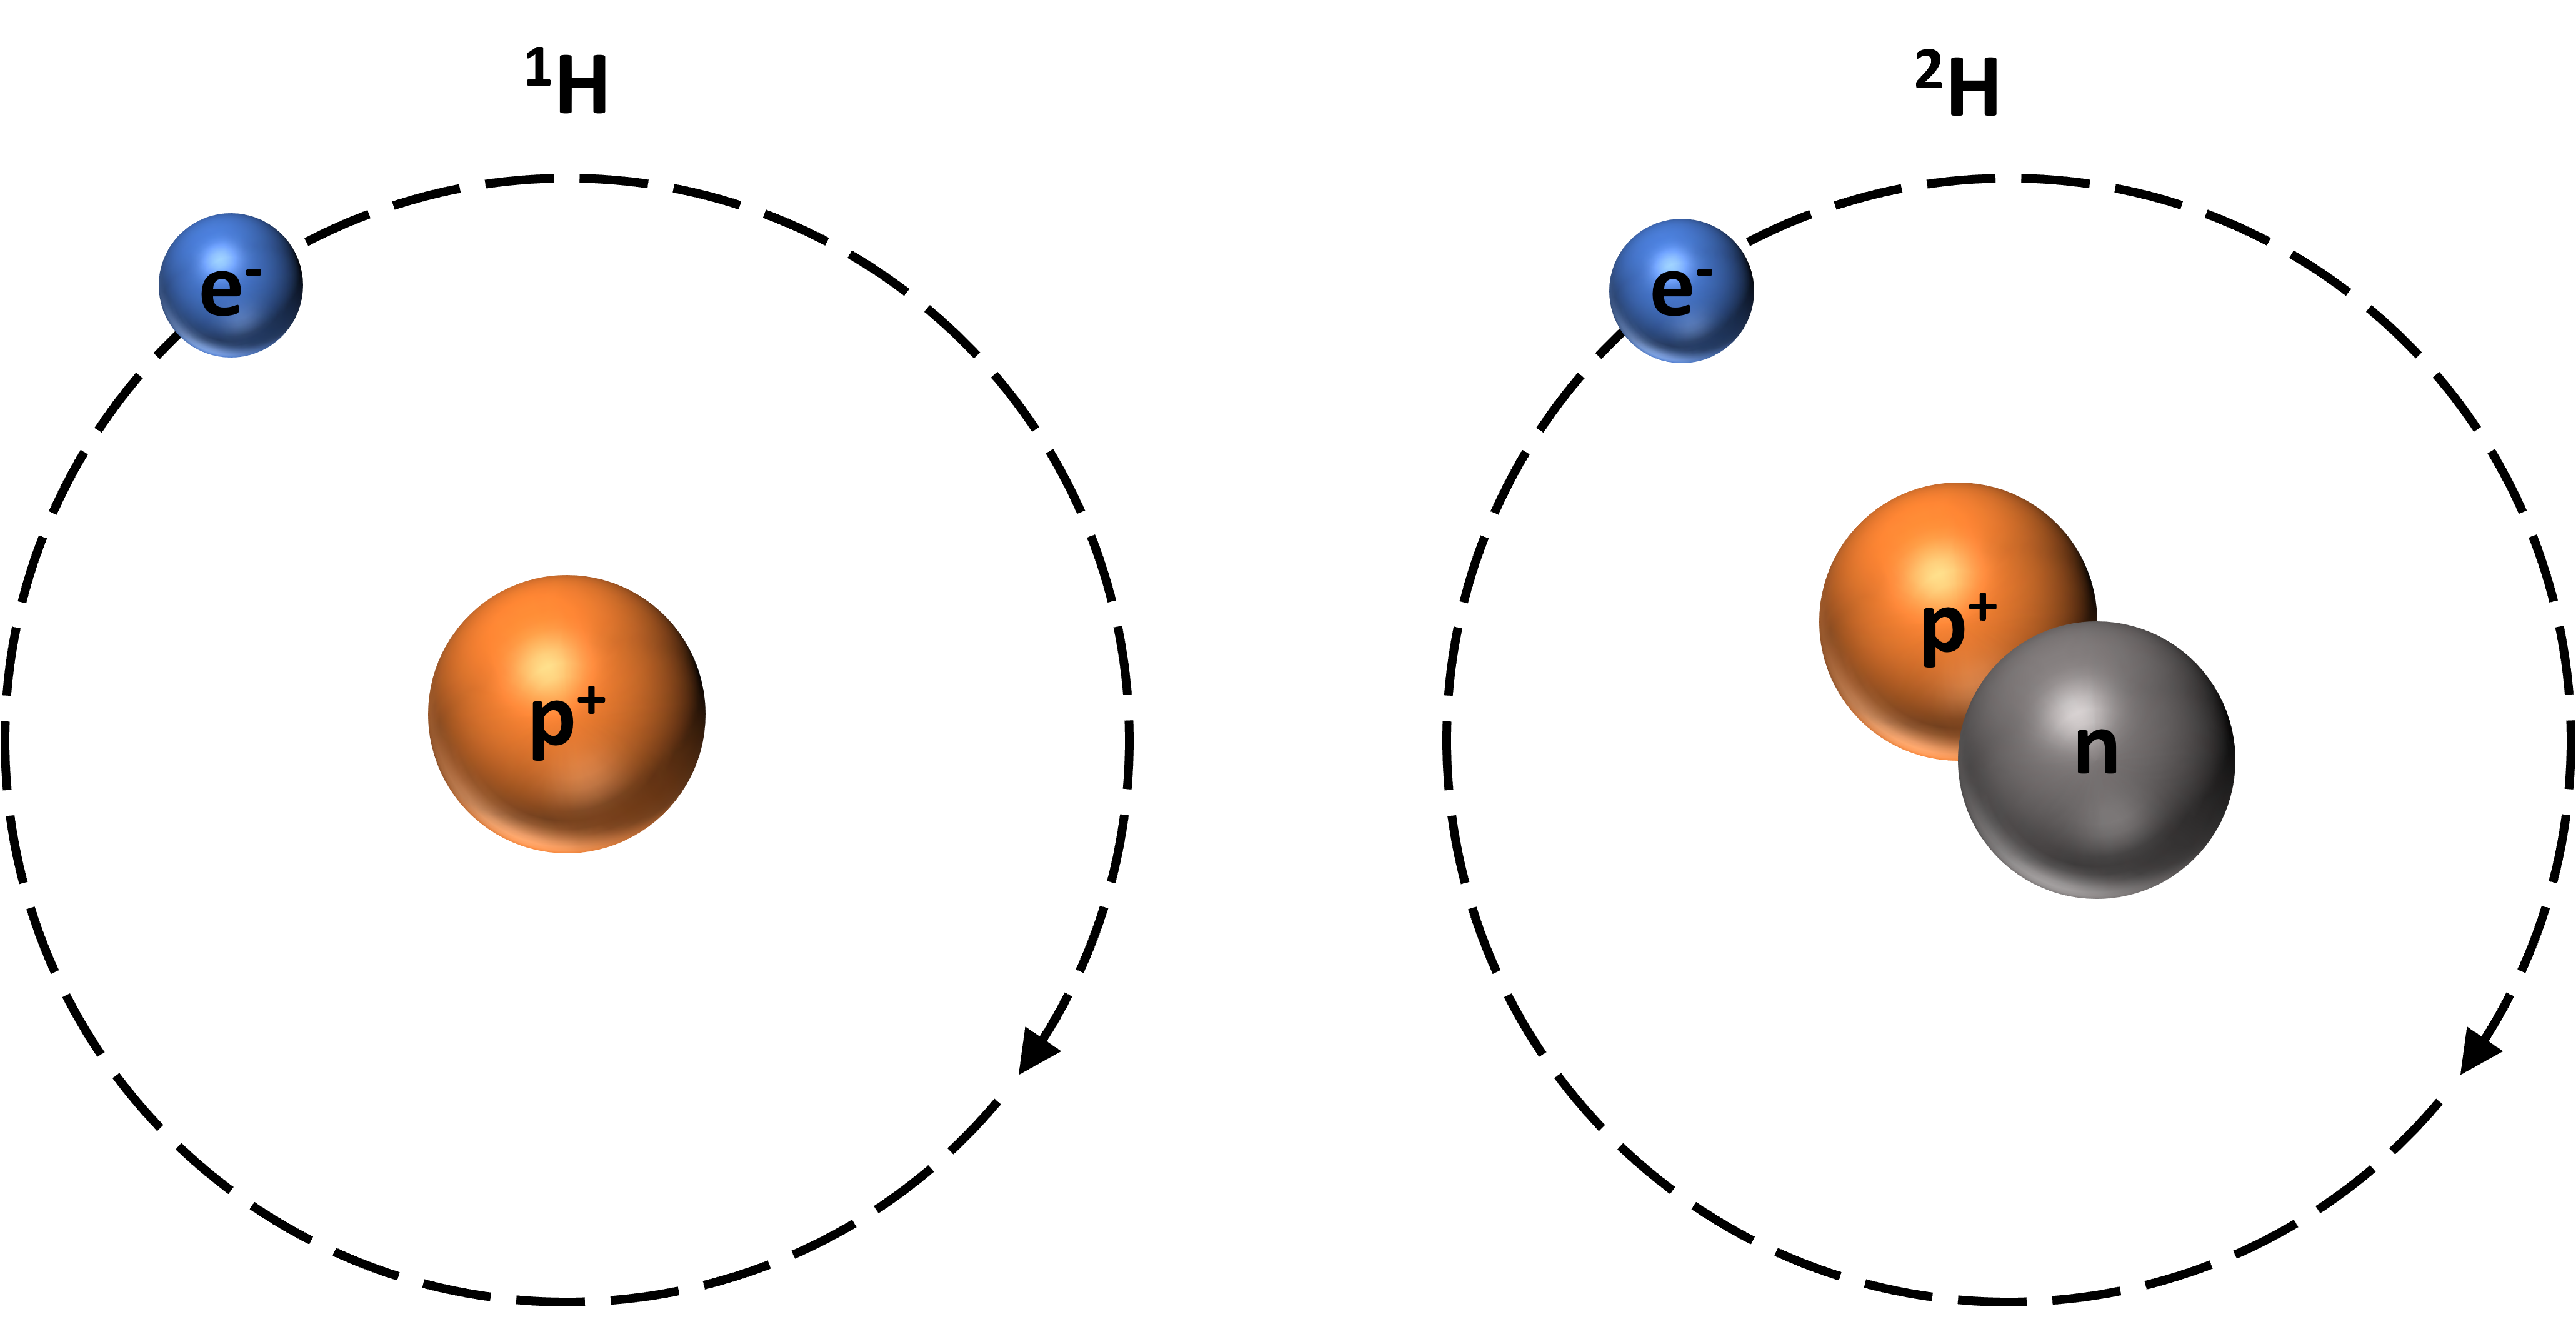
\includegraphics[width=0.9\textwidth]{Figures/Intro/1H2H.png}
    \caption{\textit{Schematic diagram of the atomic structure hydrogen ($^1$H, left) and deuterium atoms ($^2$H, right).}}
    \label{fig:intro:1H2H}
\end{figure}

\section{Metabolism}

Disrupted metabolism is a key aspect of many life-altering diseases including cancer and neurodegenerative diseases, such as \ac{AD}, \ac{PD} and \ac{MS} \cite{Gialleonardo2016TheImaging}. \ac{AD} has a European age-standardized prevalence of 4.4\% among people aged over 65 \cite{Qiu2009EpidemiologyIntervention}. One of the most prevalent and fatal metabolic diseases is cancer. In 2017 there were $\approx$375,000 new cancer cases in the UK \cite{CancerUK}, with $\approx$3\% of them being attributed to tumours in the brain and other parts of the CNS and intracranial tumours \cite{BrainUK}. The mortality rate of these cancers has remained significant and constant for the last decade \cite{BrainUK}. It is important therefore to develop tools for investigating metabolism \textit{in vivo}, and more specifically in brain tumours.

\begin{figure}
    \centering
    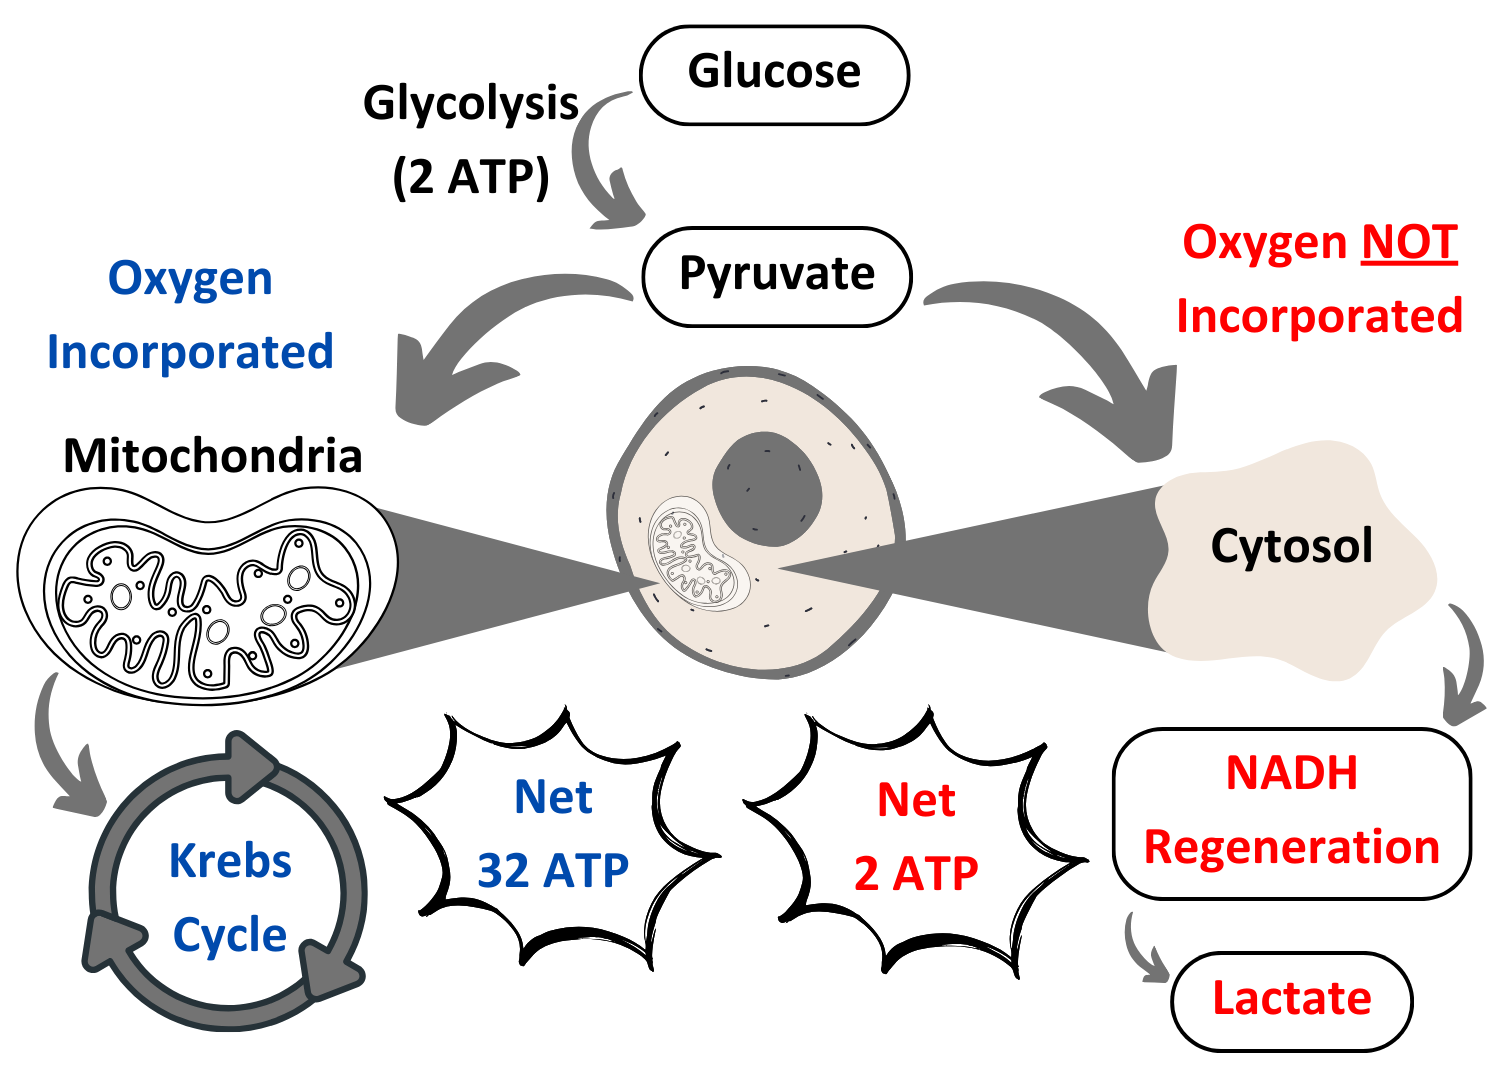
\includegraphics[width=0.75\textwidth]{Figures/Intro/Metabolism.png}
    \caption{\textit{Flow Chart demonstrating how glucose is metabolised into \ac{ATP} with (aerobic, blue) and without (anaerobic, red) oxygen being present. Healthy cells favour aerobic respiration whilst cancerous cells prefer anaerobic respiration.}}
    \label{fig:intro:Metabolism}
\end{figure}

Cancer is often considered to be a metabolic disease because as part of their growth tumours affect and impair normal metabolism. The nucleic acid \ac{ATP} is used as energy currency in cells. In mammalian cells pyruvate is generated from glucose via glycolysis and produces two molecules of \ac{ATP} per each molecule of glucose. In healthy cells there are then two options for metabolism depending on the supply of oxygen to the cell, if oxygen is readily in supply a process called oxidative-phosphorylation takes place. Oxidative-phosphorylation is where pyruvate enters the mitochondria and enters the citric acid cycle also known as the \ac{TCA} or Krebs cycle, where as many as thirty-two more \ac{ATP} are produced. This complete process is often referred to as aerobic respiration. The other option, when oxygen is not readily in supply, involves conversion of pyruvate into lactate in the cytosol of the cell through NADH regeneration. The complete process for the creation of lactate is known as lactic acid fermentation. Aerobic respiration is much more efficient in its energy production producing  around sixteen times more \ac{ATP} per mole of glucose compared to lactic acid fermentation \cite{Romero-Garcia2011TumorView}. 

\begin{figure}
    \centering
    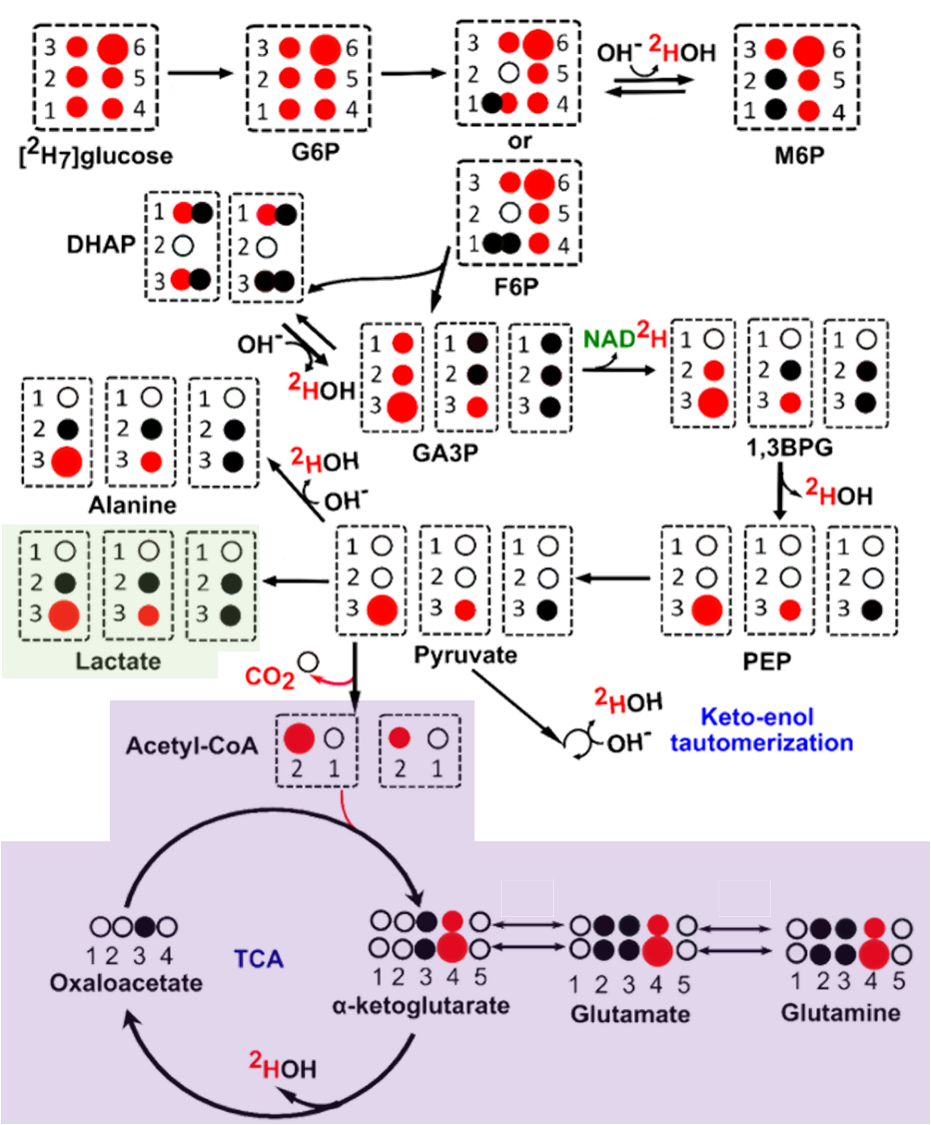
\includegraphics[width=0.9\textwidth]{Figures/Intro/D7_Metabolism.png}
    \caption{\textit{Metabolic pathway for $^2$H-labelled glucose, where all available sites for $^2$H labelling have been used. The small red circles represent individual $^2$H atoms, the large red circles represent two $^2$H atoms on the C6 and C6'. The black-filled and the empty circles represent $^1$H and quarternary carbons. The \ac{TCA} cycle is labelled on the diagram, and the specific pathway for formation of glutamate and glutamine which results from oxidative phosphorylation, is highlighted in yellow. The specific pathway for the formation on lactate resulting from lactic acid fermentation is highlighted in green. The glycolysis steps are shown from the glucose molecule to the pyruvate molecule. This figure is adapted from the figure in \cite{Mahar2021DeuteratedGlucose}.}}
    \label{fig:intro:D7Metabolism}
\end{figure}

By replacing atoms found on a glucose molecule with atoms whose presence can be tracked, it is possible to track the the glucose molecule. If the replaced atoms make there way through metabolism into downstream metabolites it can therefore inform on the metabolic pathway taken. There are seven hydrogens that are not present in hydroxyl groups in glucose which can be replaced with $^2$H atoms. During oxidative-phosphorylation, glutamate and glutamine are produced (the combination of the two is referred to as glx) and of the seven hydrogen atoms only three are transferred to glutamine/glutamate. During lactic fermentation only three of the hydrogen atoms are transferred to lactate. These hydrogens come from the C1, C6 and C6' positions in the glucose molecule. The rest of the labels (C2, C3, C4 and C5) are lost in the production of water during lactic acid fermentation and aerobic respiration. The specific metabolic pathway undertaken after fully $^2$H-labelled glucose has been ingested is outlined in Fig. \ref{fig:intro:D7Metabolism}, which shows how each $^2$H label makes it way into downstream metabolites and where the $^2$H label can be lost. It is important to note that unlabelled lactate, glutamate and glutamine can be formed from deuterated metabolites in glycolysis and by multiple iterations of the \ac{TCA} cycle. All processes take place in the cell and travel to the desired location in the blood vessels.

Otto Warburg observed in the \nth{20} century that tumours had a higher rate of glucose uptake \cite{WarburgBerlin-Dahlem1925TheCells,Warburg1956OnCells}. There were originally quite a few theories suggesting that cancerous cells had impaired the mitochondria. It is now thought that the reason behind this effect is that cancerous cells are able to metabolise by either oxidative-phosphorylation or by fermentation regardless of how much oxygen is present to the cell. Lactic fermentation is favoured to oxidative-phosphorylation even though it is less energy/\ac{ATP} efficient which therefore leads to an increase in lactate and a decrease in glx \cite{Romero-Garcia2011TumorView}.

\begin{figure}[ht]
    \centering
    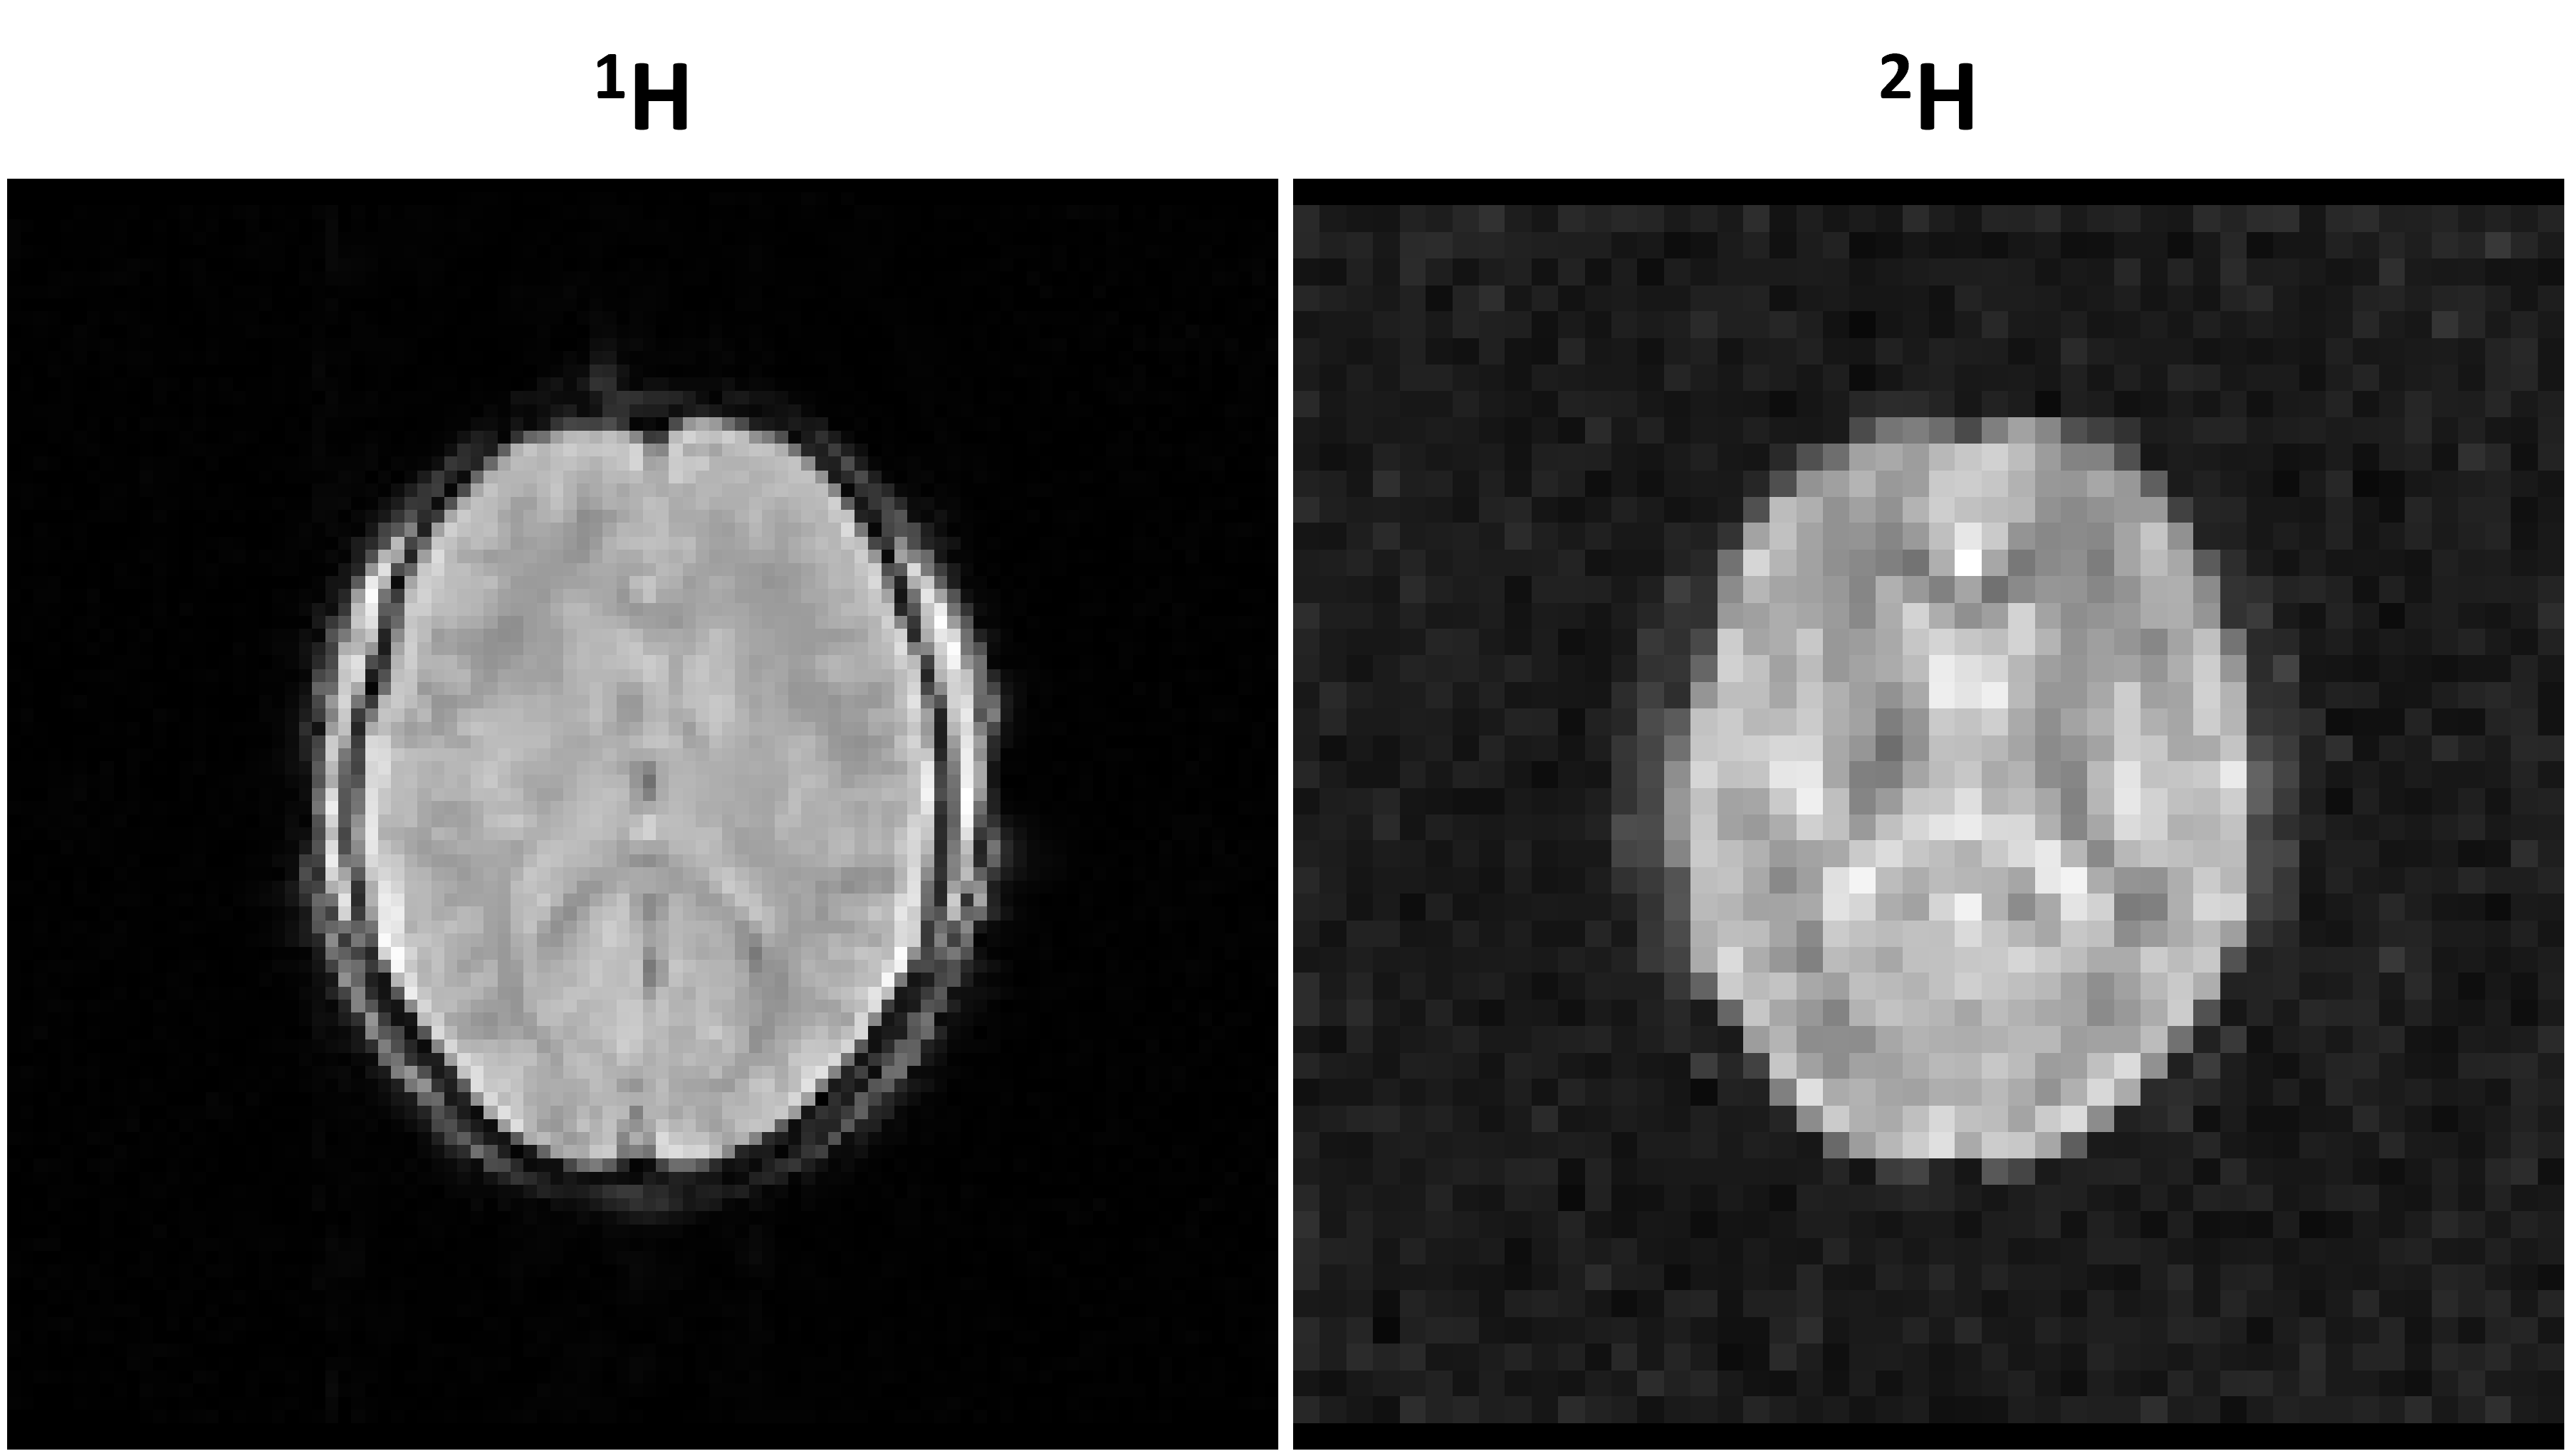
\includegraphics[width=0.9\textwidth]{Figures/Intro/1H2H_Brain.png}
    \caption{\textit{Images of the brain acquired using different nuclei, in the same scan session for the same participant using similar gradient echo sequences. Left is a $^1$H image with 3\textnormal{x}3\textnormal{x}2.5 mm$^3$ voxels acquired in 232 s. Right is a $^2$H image obtained with 6\textnormal{x}6\textnormal{x}10 mm$^3$ voxels with a scan duration of 354 s. It is important to note that the participant's $^2$H level is 100\textnormal{x}\ac{NA} as they have consumed heavy water (D$_2$O) as part of a study.}}
    \label{fig:intro:1H2H_Brain}
\end{figure}

Currently the most reliable way to accurately diagnose and monitor most cancers and metabolic diseases (such as \ac{AD} \cite{Shokouhi2014ImagingTomography} and \ac{PD} \cite{Meles2017MetabolicDisease}), in a non-invasive way, is by using \ac{PET} \cite{Almuhaideb201118F-FDGOncology}. Unfortunately this technique involves the use of a radioisotope inside the body which can put patients at further health risks, whilst a technique that is based on \ac{MRI} would be non-invasive and not require the use of ionising radiation. Cancerous cells have a much higher glucose uptake during metabolism than normal cells. This is the basis behind \ac{PET} imaging of cancer using $^{18}$F-labelled \ac{FDG}. Increased uptake of \ac{FDG} in a specific region gives an indication of the presence a cancerous tumour. \ac{FDG} \ac{PET} works by attaching a positron emitting atom to a metabolite, such as the glucose analog of \ac{FDG}, once ingested into the body it travels to the tissues where glucose is needed most. Inside cells the \ac{FDG} is phosphorylated but cannot undergo further metabolism, and so accumulates in metabolically active cells. Where the $^{18}$F-label decays, the emitted positrons annihilate with electrons, creating two photons travelling in opposite directions. These photons can be detected giving information on the location of the glucose and therefore information as to where cancer is present. A limitation of \ac{FDG} \ac{PET} is that because it only detects the presence of $^{18}$F it doesn't provide information on any downstream metabolites. Since the brain is constantly metabolically active it can often be difficult to distinguish increases in metabolism compared to baseline, this is why it is important to choose a tracer with a low abundance. Metabolite signal/concentration maps from \ac{PET} are often displayed over high resolution anatomical images to provide accurate spatial distributions.

\begin{figure}
    \centering
    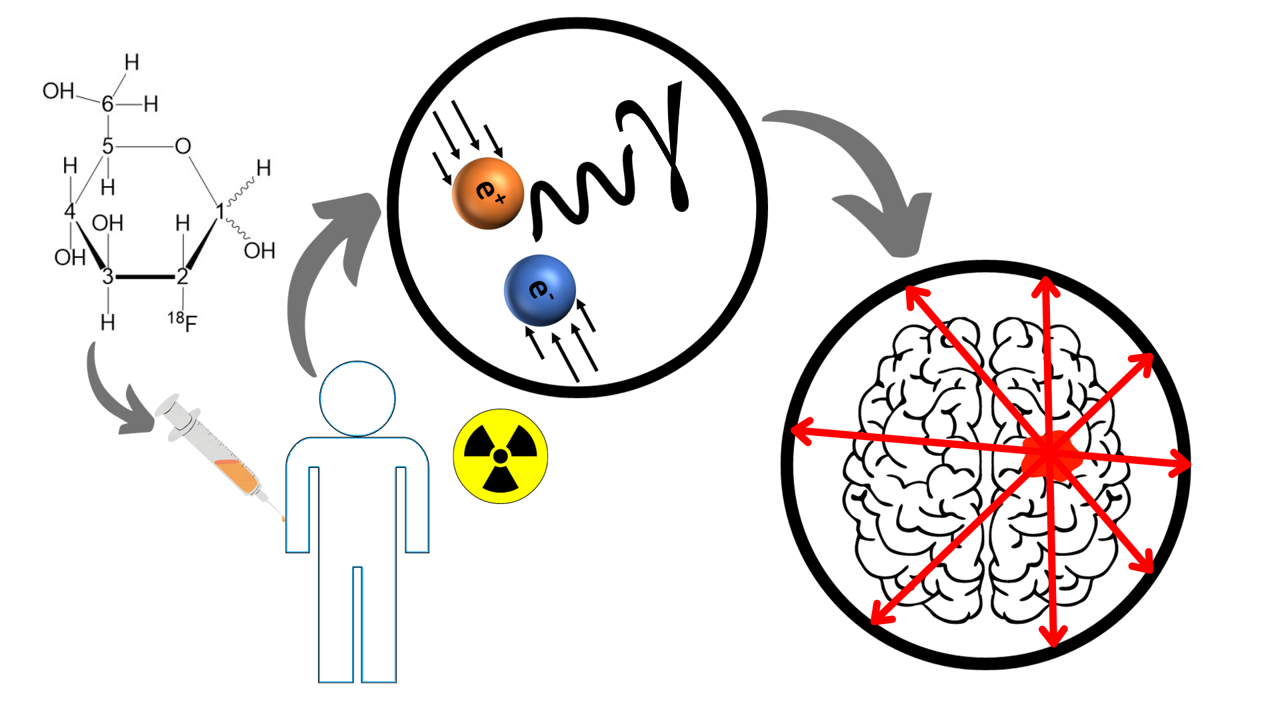
\includegraphics[width=1\textwidth]{Figures/Intro/PET_Scan.png}
    \caption{\textit{Diagram showing how \ac{PET} scanning works at detecting tumours.}}
    \label{fig:intro:PET}
\end{figure}

\section{History of $^2$H Usage in Studying Metabolism}

\subsection{Pre-1980}

$^2$H was discovered in 1932 \cite{Urey1932AConcentration} from consideration of the apparent mass difference of hydrogen when measured chemically and with a mass spectrograph. It was rapidly realised that this stable isotope could be used to measure metabolism. Many papers were published demonstrating this \cite{Schoenheimer1935DeuteriumMetabolism,Schoenheimer1938TheMetabolism} for example via deuterating naturally occurring compounds such as fatty acids, feeding them to animals and then analysing the amount of deuterium found in bodily fluids. Shortly after this the relaxation properties of $^2$H in \ac{NMR} were quantified in a solution of heavy water \cite{Bloembergen1948RelaxationAbsorption}. One possible explanation as to why it then took so long for this technique combined with \ac{NMR} to become popular is due to the rising interest (at the time) \cite{DeFeyter2021DeuteriumFuture} in use of radioactive isotopes $^3$H \cite{Thompson1953StudiesRat} and $^{14}$C \cite{Turteltaub1990AcceleratorDNA.} for metabolic studies. The health concerns around use of radioactive isotopes led to a resurgence of $^2$H metabolism research in the 1980's.

\subsection{1980 to the 21\textsuperscript{st} Century}

% Graphs of fat lipid changes from paper or from our own NA work 

\begin{figure}
    \centering
    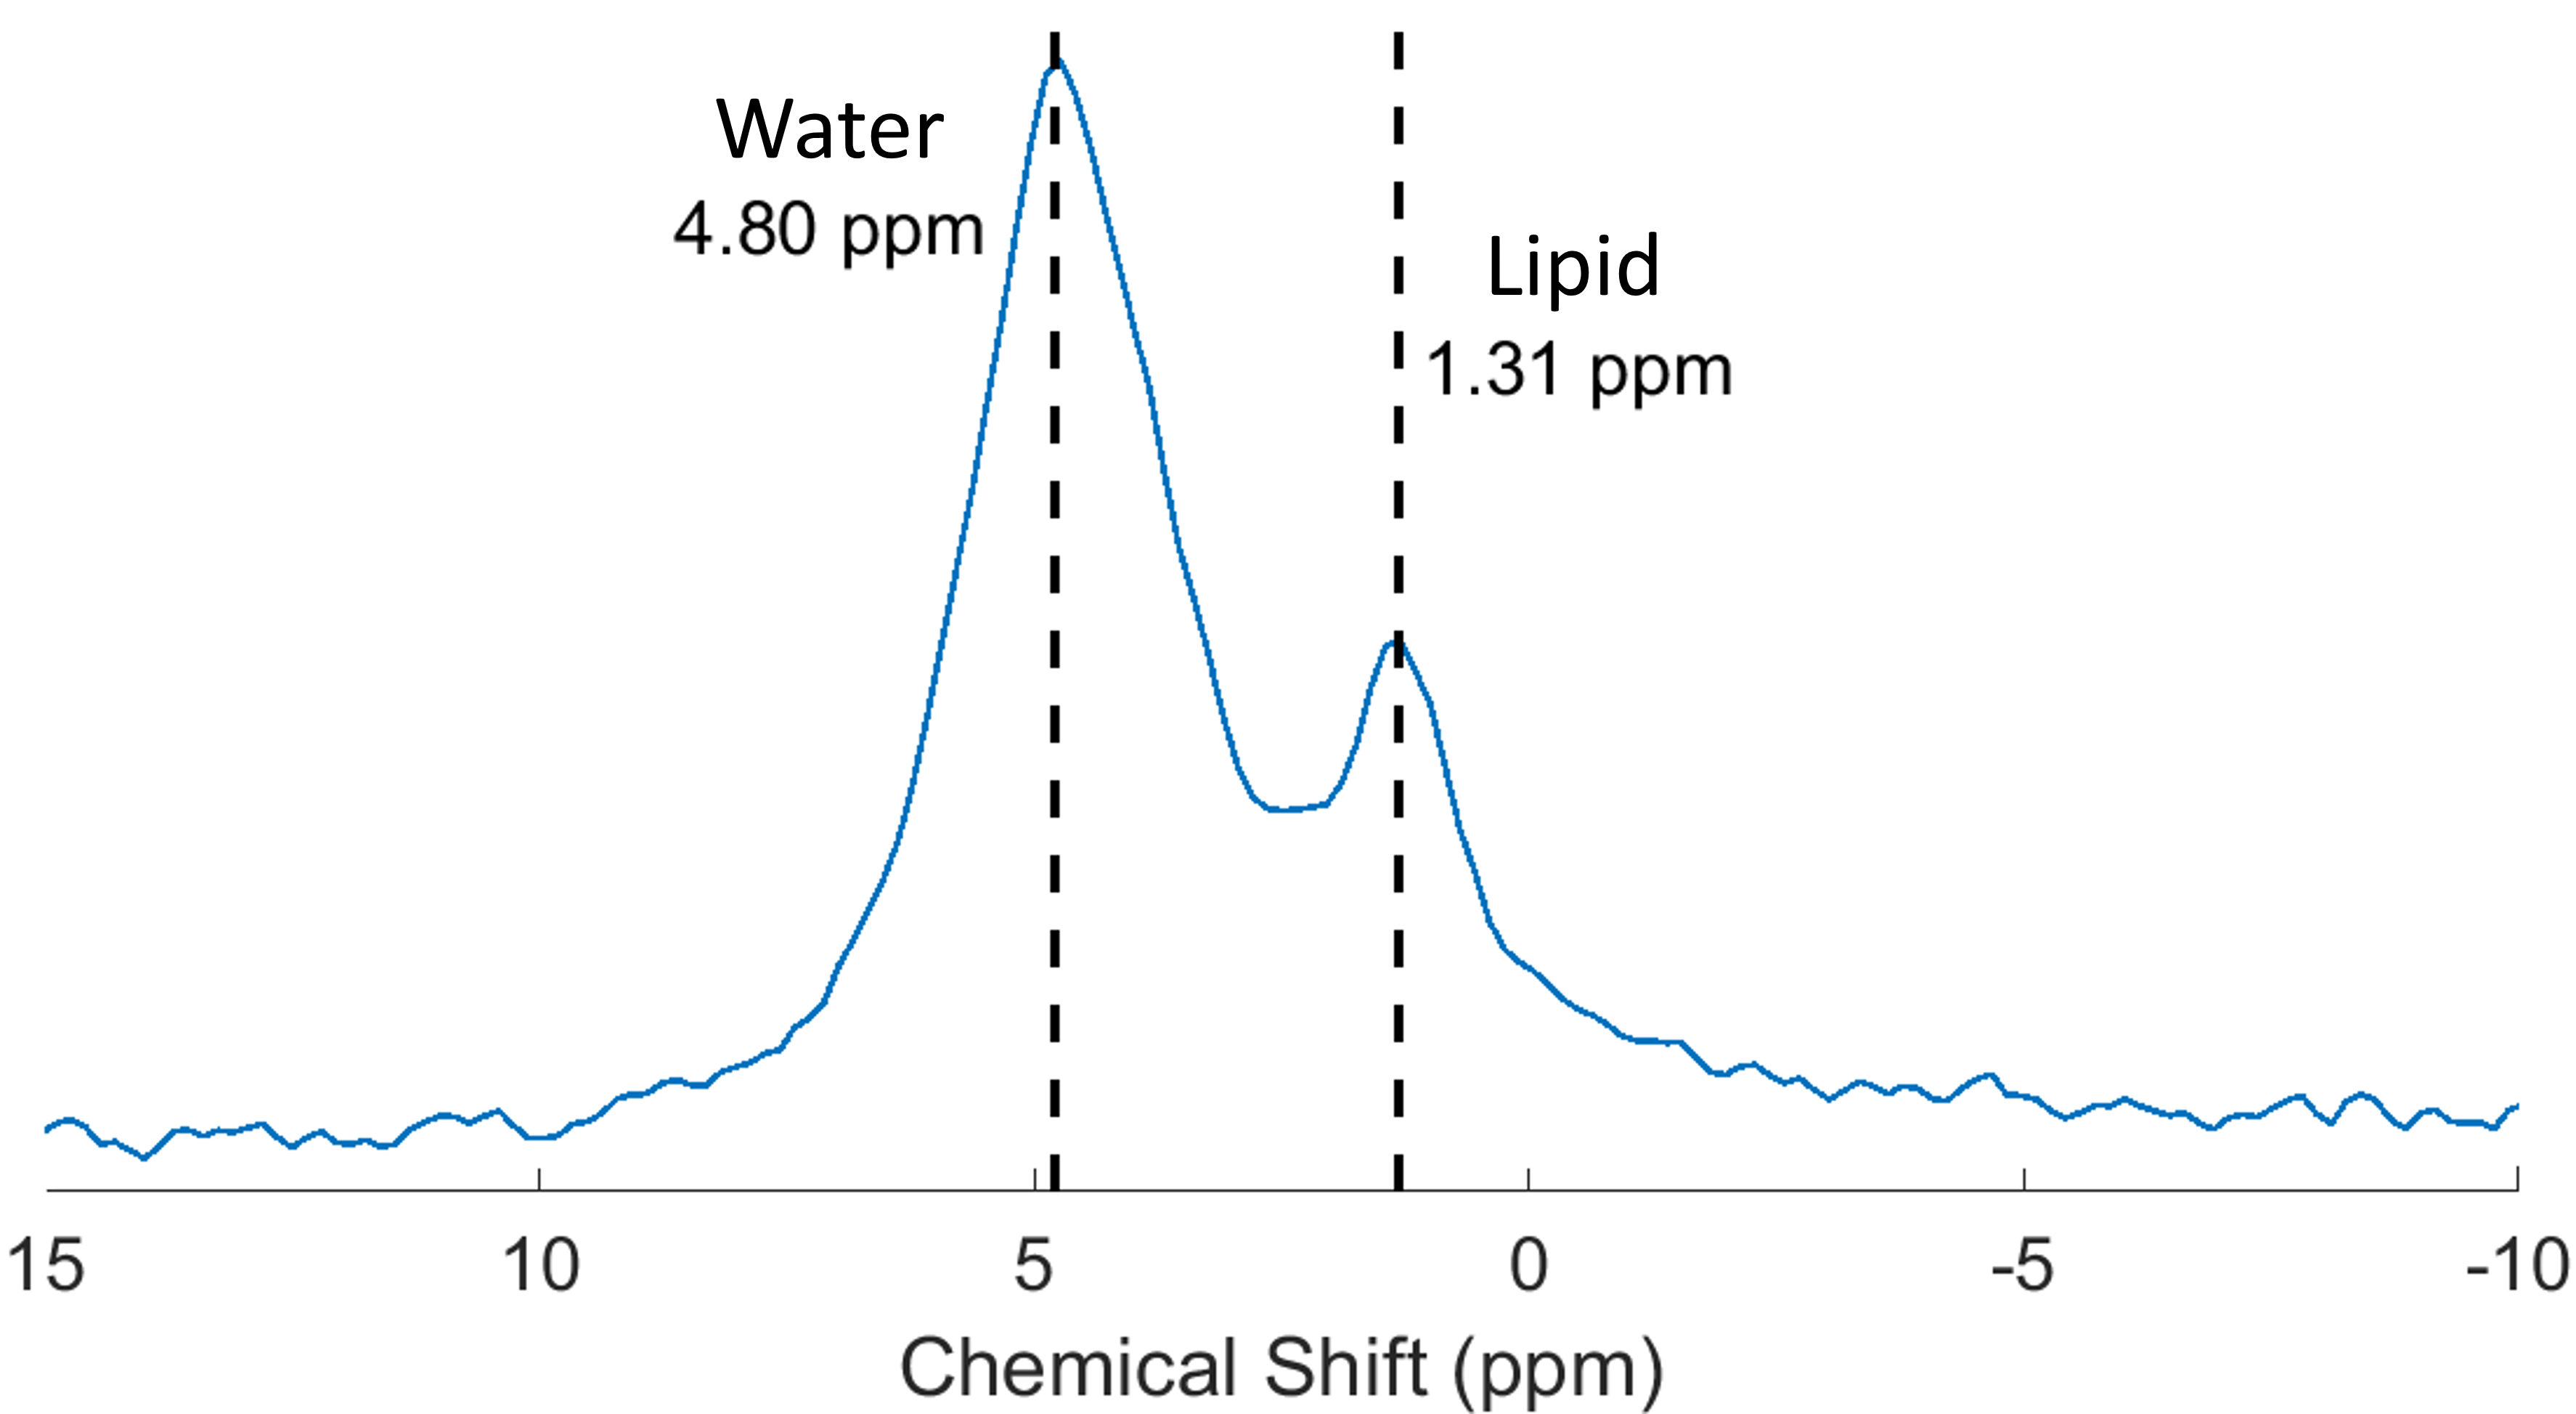
\includegraphics[width=0.8\textwidth]{Figures/Intro/NA_Spectra.png}
    \caption{\textit{Non-localised $^2$H spectra obtained from the calf \textit{in vivo} showing signals from water at a chemical shift of 4.8 ppm and fat/lipid signals at 1.3 ppm.}}
    \label{fig:intro:NA}
\end{figure}

The first \textit{in vivo} $^2$H NMR study was performed in 1986 \cite{Brereton1986PreliminarySpectroscopy} in mice. \Ac{D$_2$O} ingestion was used to increase $^2$H abundance, and an increase in fat/lipid signal was measured. Shortly after this numerous pre-clinical studies were published that involved using heavy water as a tracer, looking at: the brain \cite{Ewy1988DeuteriumSitu}, blood flow and perfusion \cite{Ackerman1987DeuteriumTracer.} and iron stores \cite{Irving1987InSpectroscopy}. Other deuterated compounds then started to be used such as choline \cite{Eng1990RenalStudy}, with the first instance of deuterated glucose being used being in 1986 \cite{Barrow1986NMRMobilis}. This started a trend of other studies using deuterated glucose to investigate bacterial metabolism \cite{Aguayo1988HighMetabolism.} and liver gycogen synthesis \cite{Goodman1989UseSynthesis}. All the aforementioned studies involved animal models, the amount of studies that involved $^2$H then slowed down before a long hiatus. One potential reason for this hiatus was the success' of \textit{in vivo} $^1$H \cite{Harada1984IdentificationScience}, $^{13}$C \cite{Cohen1980UseLiver} and $^{31}$P \cite{Sappey-Marinier1992EffectSpectroscopy} measurements. However, there has recently been a resurgence in $^2$H MR research and more specifically its use in studying metabolism.

\subsection{The Last Seven Years}

\begin{figure}[H]
    \centering
    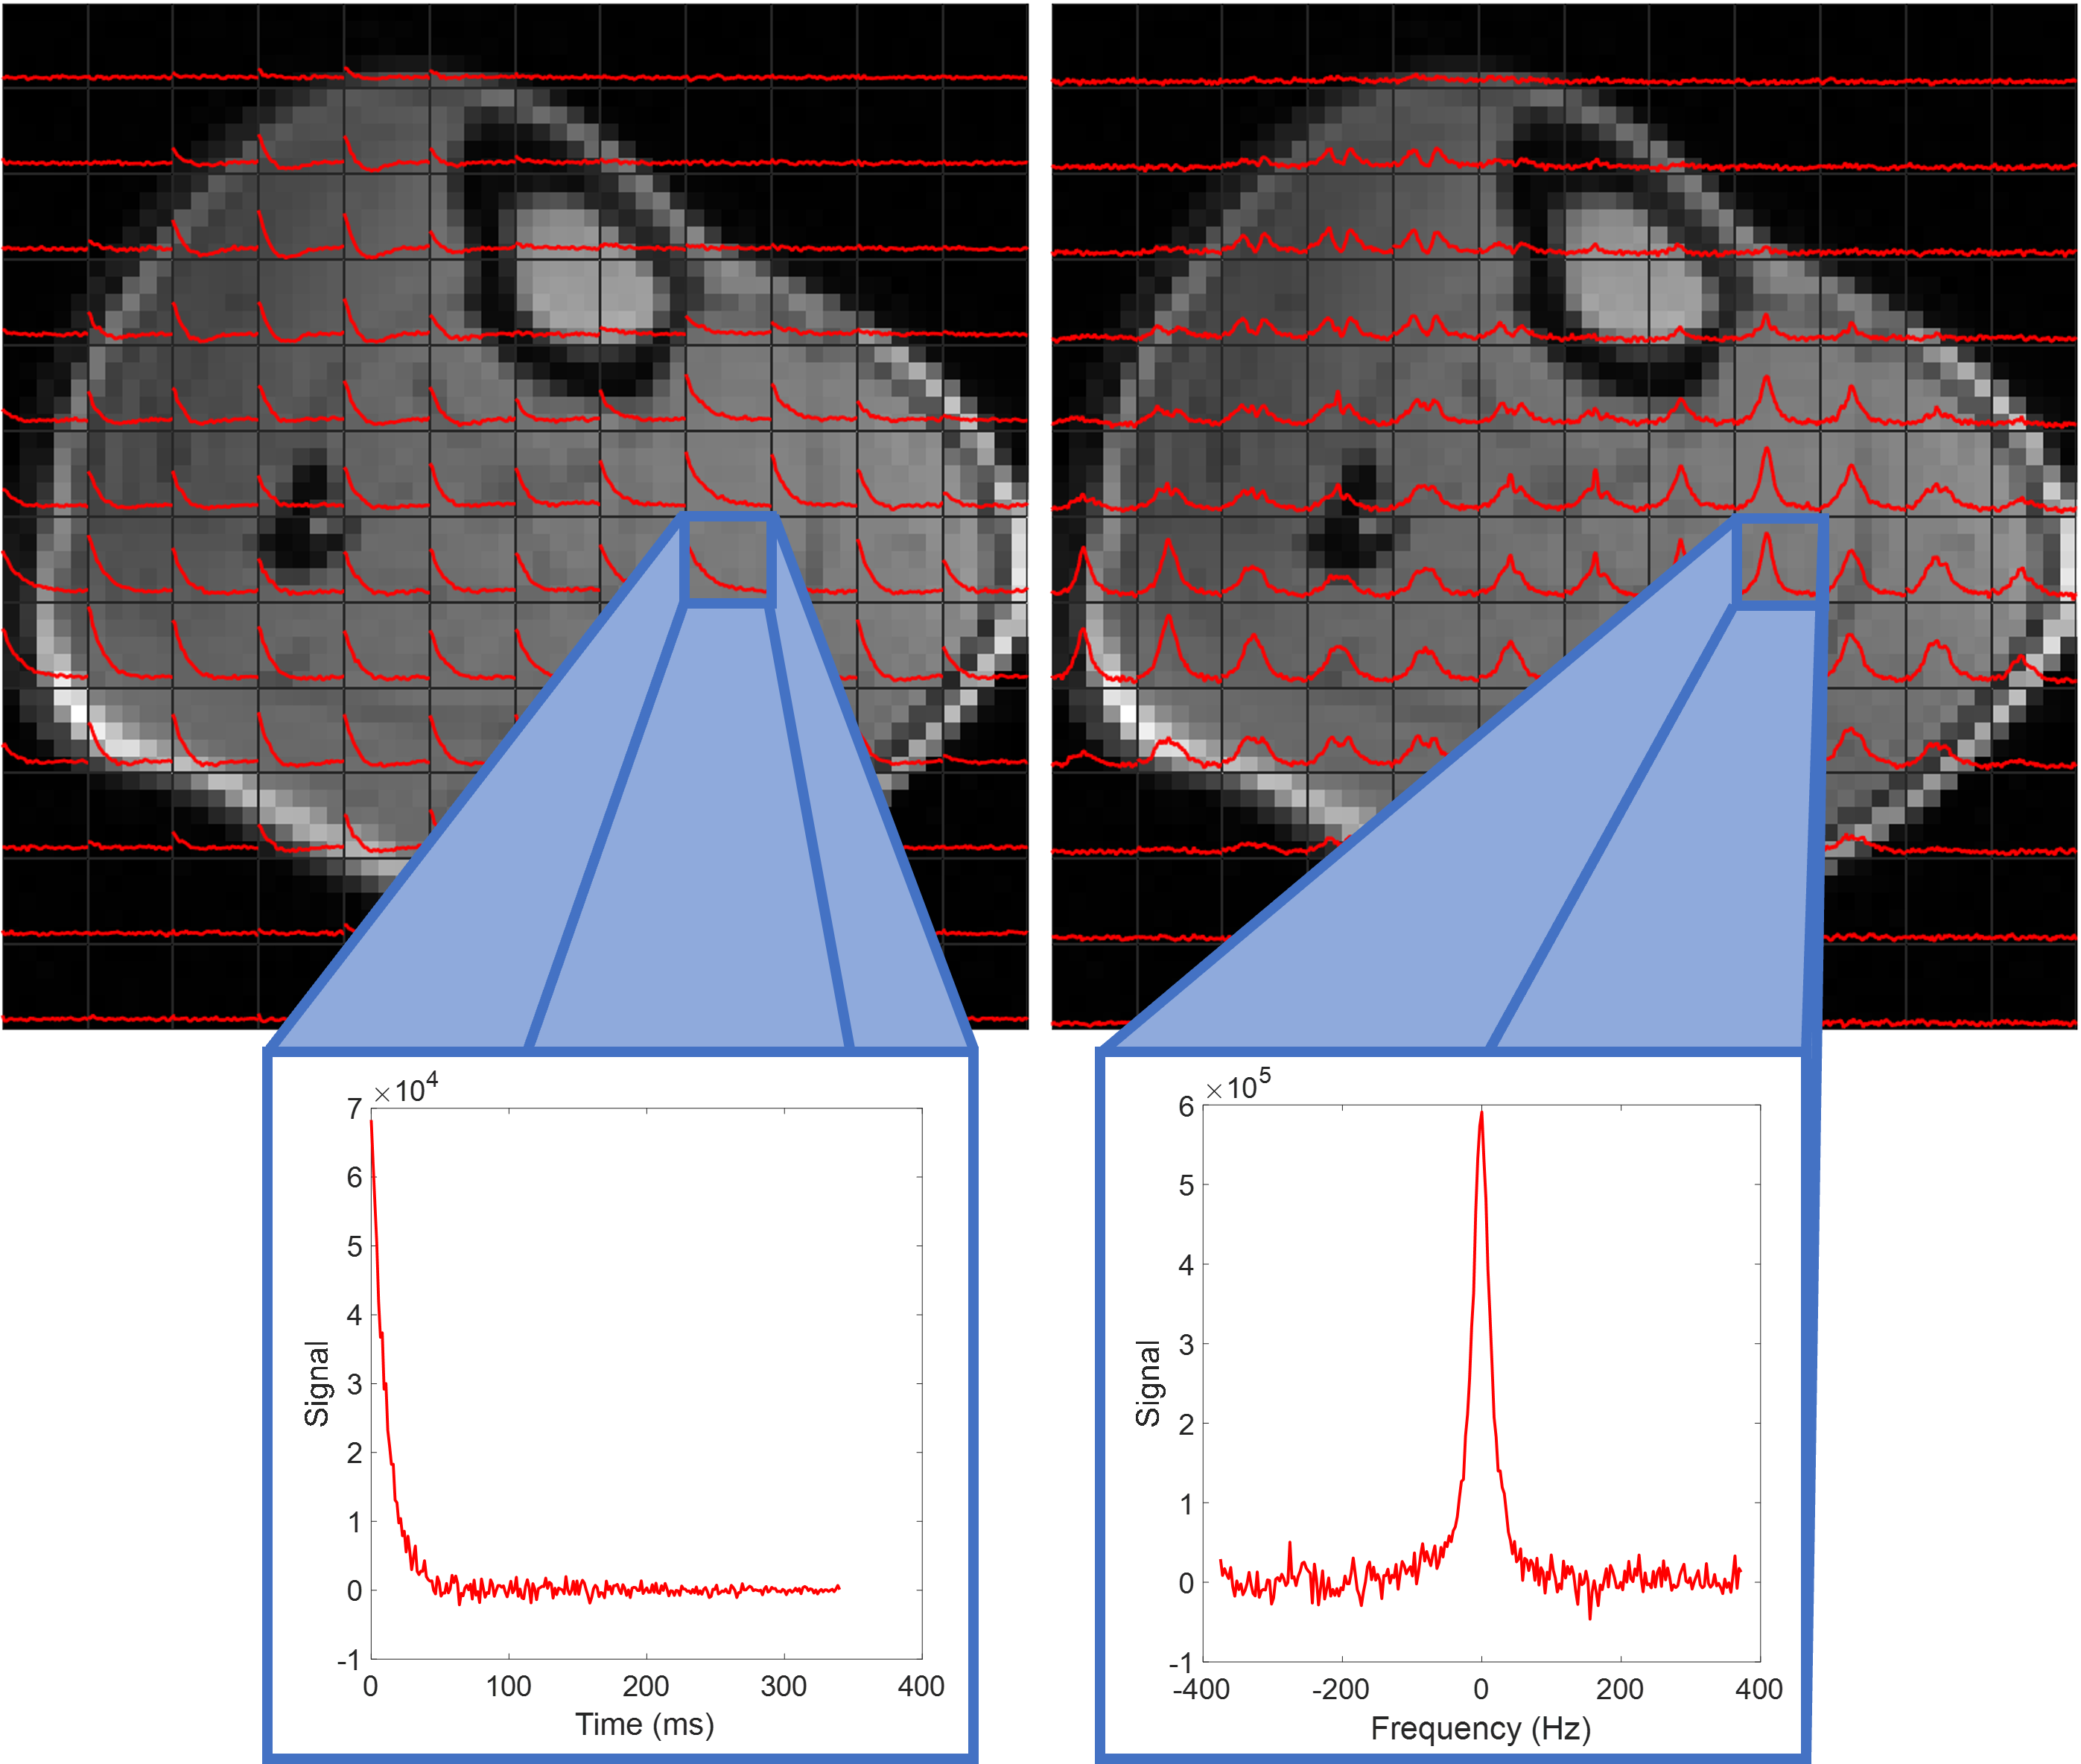
\includegraphics[width=0.8\textwidth]{Figures/Intro/CSI.png}
    \caption{\textit{Example \ac{NA} \ac{MRSI} data overlayed onto an anatomical image of the Calf. The left shows the localised \ac{FID} data from voxels with one voxel blown up. The right shows the corresponding localised spectroscopic data (Fourier transform of the \ac{FID} shown on the left) with data from one voxel blown up.}}
    \label{fig:intro:CSI}
\end{figure}

[6,6'-$^2$H$_2$] (also known as $^2$H$_2$-glucose or D$_2$-glucose) was first used \textit{in vivo} in an animal model \cite{Lu2017QuantitativeSpectroscopy} in 2017, where both the $^1$H atoms at C6 and C6' are replaced with $^2$H. And soon after this technique was applied \textit{in vivo} in humans, where it was demonstrated that differences between normal and tumour tissue could be seen in maps of $^2$H signals from downstream metabolic products of the labelled glucose \cite{DeFeyter2018DeuteriumVivo}. This form of glucose is currently the most commonly used deuterated tracer in research \cite{DeFeyter2018DeuteriumVivo,DeFeyter2021DeuteriumFuture,Ruhm2022Dynamic9.4T,Roig2022Deuterium7T,deGraaf2020OnImaging}. At \ac{NA} only a deuterated water (HDO) peak/signal is visible in a typical spectrum, because the noise level is higher than the signals from other $^2$H in other molecules. After ingestion of D$_2$-glucose, peaks from deuterated glucose (Glu), a combination of glutamine and glutamate (Glx) and lactate (Lac) appear. \ac{CSI} or other \ac{MRSI} methods, can be used to produce maps of each of these metabolites. Production of maps of the ratio of the Glx and Lac concentration have been shown to provide a good delineation of cancerous tissue \cite{DeFeyter2018DeuteriumVivo,Straathof2021DeuteriumBrain}. Other deuterated compounds have been used to measure different metabolic pathways. These include [$^2$H$_3$]-acetate (D$_3$-acetate) \cite{DeFeyter2018DeuteriumVivo,Rich20201HVivo}, [6,6'-$^2$H$_2$]-fructose (D$_2$-fructose) \cite{Zhang202366-2H2Cancer}, as well as other forms of deuterated glucose. For example [2,3,4,6,6'-$^2$H$_5$] (D$_5$-glucose) \cite{Zou2023AImaging} has been found to be cheaper to provide than D$_2$-glucose.

% De Feyter images or CSI images

\section{Aims}

The aims of the work described in this thesis are to develop $^2$H \ac{MRI} and \ac{MRSI} scanning at the \ac{SPMIC} at the University of Nottingham at both clinical high field (3T) and ultra-high field (7T). Work outlined in this thesis is relevant for the implementation of $^2$H at a range of field strengths. The more specific primary aim of the work described in this thesis is to set the ground for scanning patients with brain tumours using DMI at 7T.

All the work that is outlined in this thesis involves the use of 
 $^2$H \ac{MRI} and \ac{MRSI} techniques and includes: measuring the relaxation times of \ac{HDO} in different healthy \textit{in vivo} brain tissues; assessing the increase in $^2$H abundance as \Ac{D$_2$O} is ingested in in different healthy \textit{in vivo} brain tissues; using different amounts of $^2$H labelling of glucose to assess \textit{in vivo} metabolism in the brain of healthy participants; evaluating whether the ingestion of \Ac{D$_2$O} in conjunction with $^2$H MR can be used to investigate lipid turnover; using $^2$H MR following ingestion of \Ac{D$_2$O} to assess the quadrupolar \ac{HDO} splitting in anisotropic and isotropic tissues using regular \ac{MRI} and \ac{MRSI}, as well as double-quantum-filtered \ac{MRI} and MRSI.

\section{Description of Work}

Chapter two covers the theory underlying the work that was undertaken in this thesis. This includes the theory behind \ac{MRI} and \ac{MRSI} and more specifically the difference between $^1$H and $^2$H \ac{NMR} including magnetisation, relaxation and pulse sequences. This chapter also describes the extra hardware adaptations that are needed for $^2$H signal detection, ranging from amplifiers to \ac{RF} coil building.

Chapter three reports the first measurements of $^2$H signals from the brain in subjects who had ingested heavy water. A \ac{D$_2$O} ingestion routine is outlined, as well as a scanning routine undertaken to allow the quantification of $^2$H relaxation times in the human brain using \ac{MEGE} scans with different \ac{TR}-values. Similar scans were then also used for some participants to track the $^2$H increase that occurs immediately following the ingestion of \ac{D$_2$O}. It was shown that the $^2$H increase from \ac{MRI}/\ac{MRS} follows what is expected from blood sampling, and the relaxation times for different tissues are reported with statistical significance shown.

% Chapter four gives an overview of some of the research that has been conducted so far in deuterium metabolic imaging (DMI) predicts the potential benefits of using D$_7$-glucose as opposed to D$_2$-glucose. 

Chapter four describes the first measurements of metabolism in human subjects using \ac{DMI} with D$_7$-glucose. The methodology used so healthy participants can ingest deuterated glucose is outlined as well as the scanning routine with parameters for CSI scanning. Increases in signal levels for all downstream metabolites resulting from the D$_7$-glucose were found which suggests better \ac{CNR} between healthy and tumour tissue would be possible, despite the more complicated analysis.

Chapter five describes the importance of measuring lipid turnover and the limitations of the present methodology involving heavy-water loading and biopsy, and suggests a new routine that uses $^2$H \ac{MRI}/\ac{MRS} instead. A new routine of ingesting \ac{D$_2$O} is given as well as regular scanning routine that is repeated once a fortnight. Increases in $^2$H lipid were seen in most the measurements with statistical significance, but new advances/improvements are needed to make this technique is clinically viable.

Chapter six describes an investigation of the quadrupolar splitting seen in the $^2$H signal from water in muscle, where the orientation of the muscle relative the external magnetic field affects the splitting amplitude. After participants have their $^2$H abundance increased by ingesting \ac{D$_2$O}, \ac{MRSI} and \ac{DQF} \ac{MRSI} have been used to show the relationship between the anisotropy and quadrupolar interaction in the forearm and the calf.

Finally, chapter seven brings together all the work that has been conducted in this thesis, and gives direction on any future work that may be conducted.

\newpage
\chapter{Theory}
\label{Chap:Theory}

\section{How \ac{NMR} Works}
\subsection{Quantum Behaviour}

Many subatomic particles have a quantum `spin' and its important to note that whilst the `rotation' does not scale to the macroscopic world, a strong analogy can be made to macroscopic spin to explain the physics behind their behaviour in the quantum world. This spin is linked to an angular momentum defined by the operator J, which is made up of orbital angular momentum ($\mathbf{L} = \mathbf{r}\, \textrm{x} \, \mathbf{p}$, $\mathbf{r}$ is position $\mathbf{p}$ is momentum) as well as spin angular momentum ($\mathbf{S}$ for total spin and $m_s$ for z-component). The spin of sub-atomic particles is associated with a magnetic moment. The atomic nucleus can therefore be represented to a magnetic dipole (which is analogous to an electric dipole) which tend to align with external magnetic fields. The magnetic moment ($\mathbf{\mu}$) of a nucleus is dependent on its spin as shown in Eq. \ref{eqn:theory:moment}.

\begin{equation}
    \mathbf{\mu} = \frac{g_sq}{2m} \mathbf{S}
    \label{eqn:theory:moment}
\end{equation}

Here, $\mathbf{S}$ is the spin angular momentum, $q$ is the charge, $g_s$ is dimensionless and is known as the spin g-factor and $m$ is the mass. The constant of proportionality linking the magnetic moment to the spin is known as the gyromagnetic ratio ($\gamma$) and is a constant for each nucleus. 

\begin{equation}
    \gamma = \frac{g_sq}{2m}
    \label{eqn:theory:gyro}
\end{equation}

When a nucleus is exposed to an external static magnetic field ($\mathbf{B}$) it will possess an energy according to Eq. \ref{eqn:theory:ESpin} which is also dependent on $\mu$.

\begin{equation}
    E = \mathbf{\mu} \cdot \mathbf{B}
\end{equation}

In 1922 an experiment was undertaken \cite{Gerlach1922DerMagnetfeld} which showed that spin only takes specific discrete values ($s =$ 0, 1/2, 1, 3/2 ...), which gives eigenvalues for the angular momentum operator $\mathbf{S}$ as $\hbar m_s$. Where $m_s$ can take values of $-s$ to $+s$ in integer steps. Therefore, the magnetic moment and the energy will also take specific discrete energy levels.

\begin{equation}
    E = -m_s\hbar \gamma B_0
    \label{eqn:theory:ESpin}
\end{equation}

This is evident in Fig. \ref{fig:theory:zeeman}. The energy of an electromagnetic photon is directly proportional to its frequency ($f$), with a constant of proportionality equal to Planck's constant $h$, this is known as the Planck relation. Therefore, an absorbed photon will need a minimum energy equal to the separation between these quantified energy states, this relationship is shown in Eq. \ref{eqn:theory:ELamor}.

\begin{equation}
    \Delta E = hf = \frac{h}{2\pi}\gamma B_0
    \label{eqn:theory:ELamor}
\end{equation}  

The nucleus' frequency of precession here is therefore directly proportional to the magnitude of the applied external magnetic field ($B_0$), with $\gamma$ being the constant of proportionality meaning this frequency is also specific to each nucleus. This frequency is called the Larmor frequency \cite{Larmor1897LXIII.Ions} and is often represented as an angular frequency ($\omega$). This therefore shows that for a nucleus with spin the energy, frequency and applied magnetic field share a quantum relationship. 

\begin{equation}
    \omega = \gamma B_0
    \label{eqn:theory:Lamor}
\end{equation}

\begin{figure}[h]
    \centering
    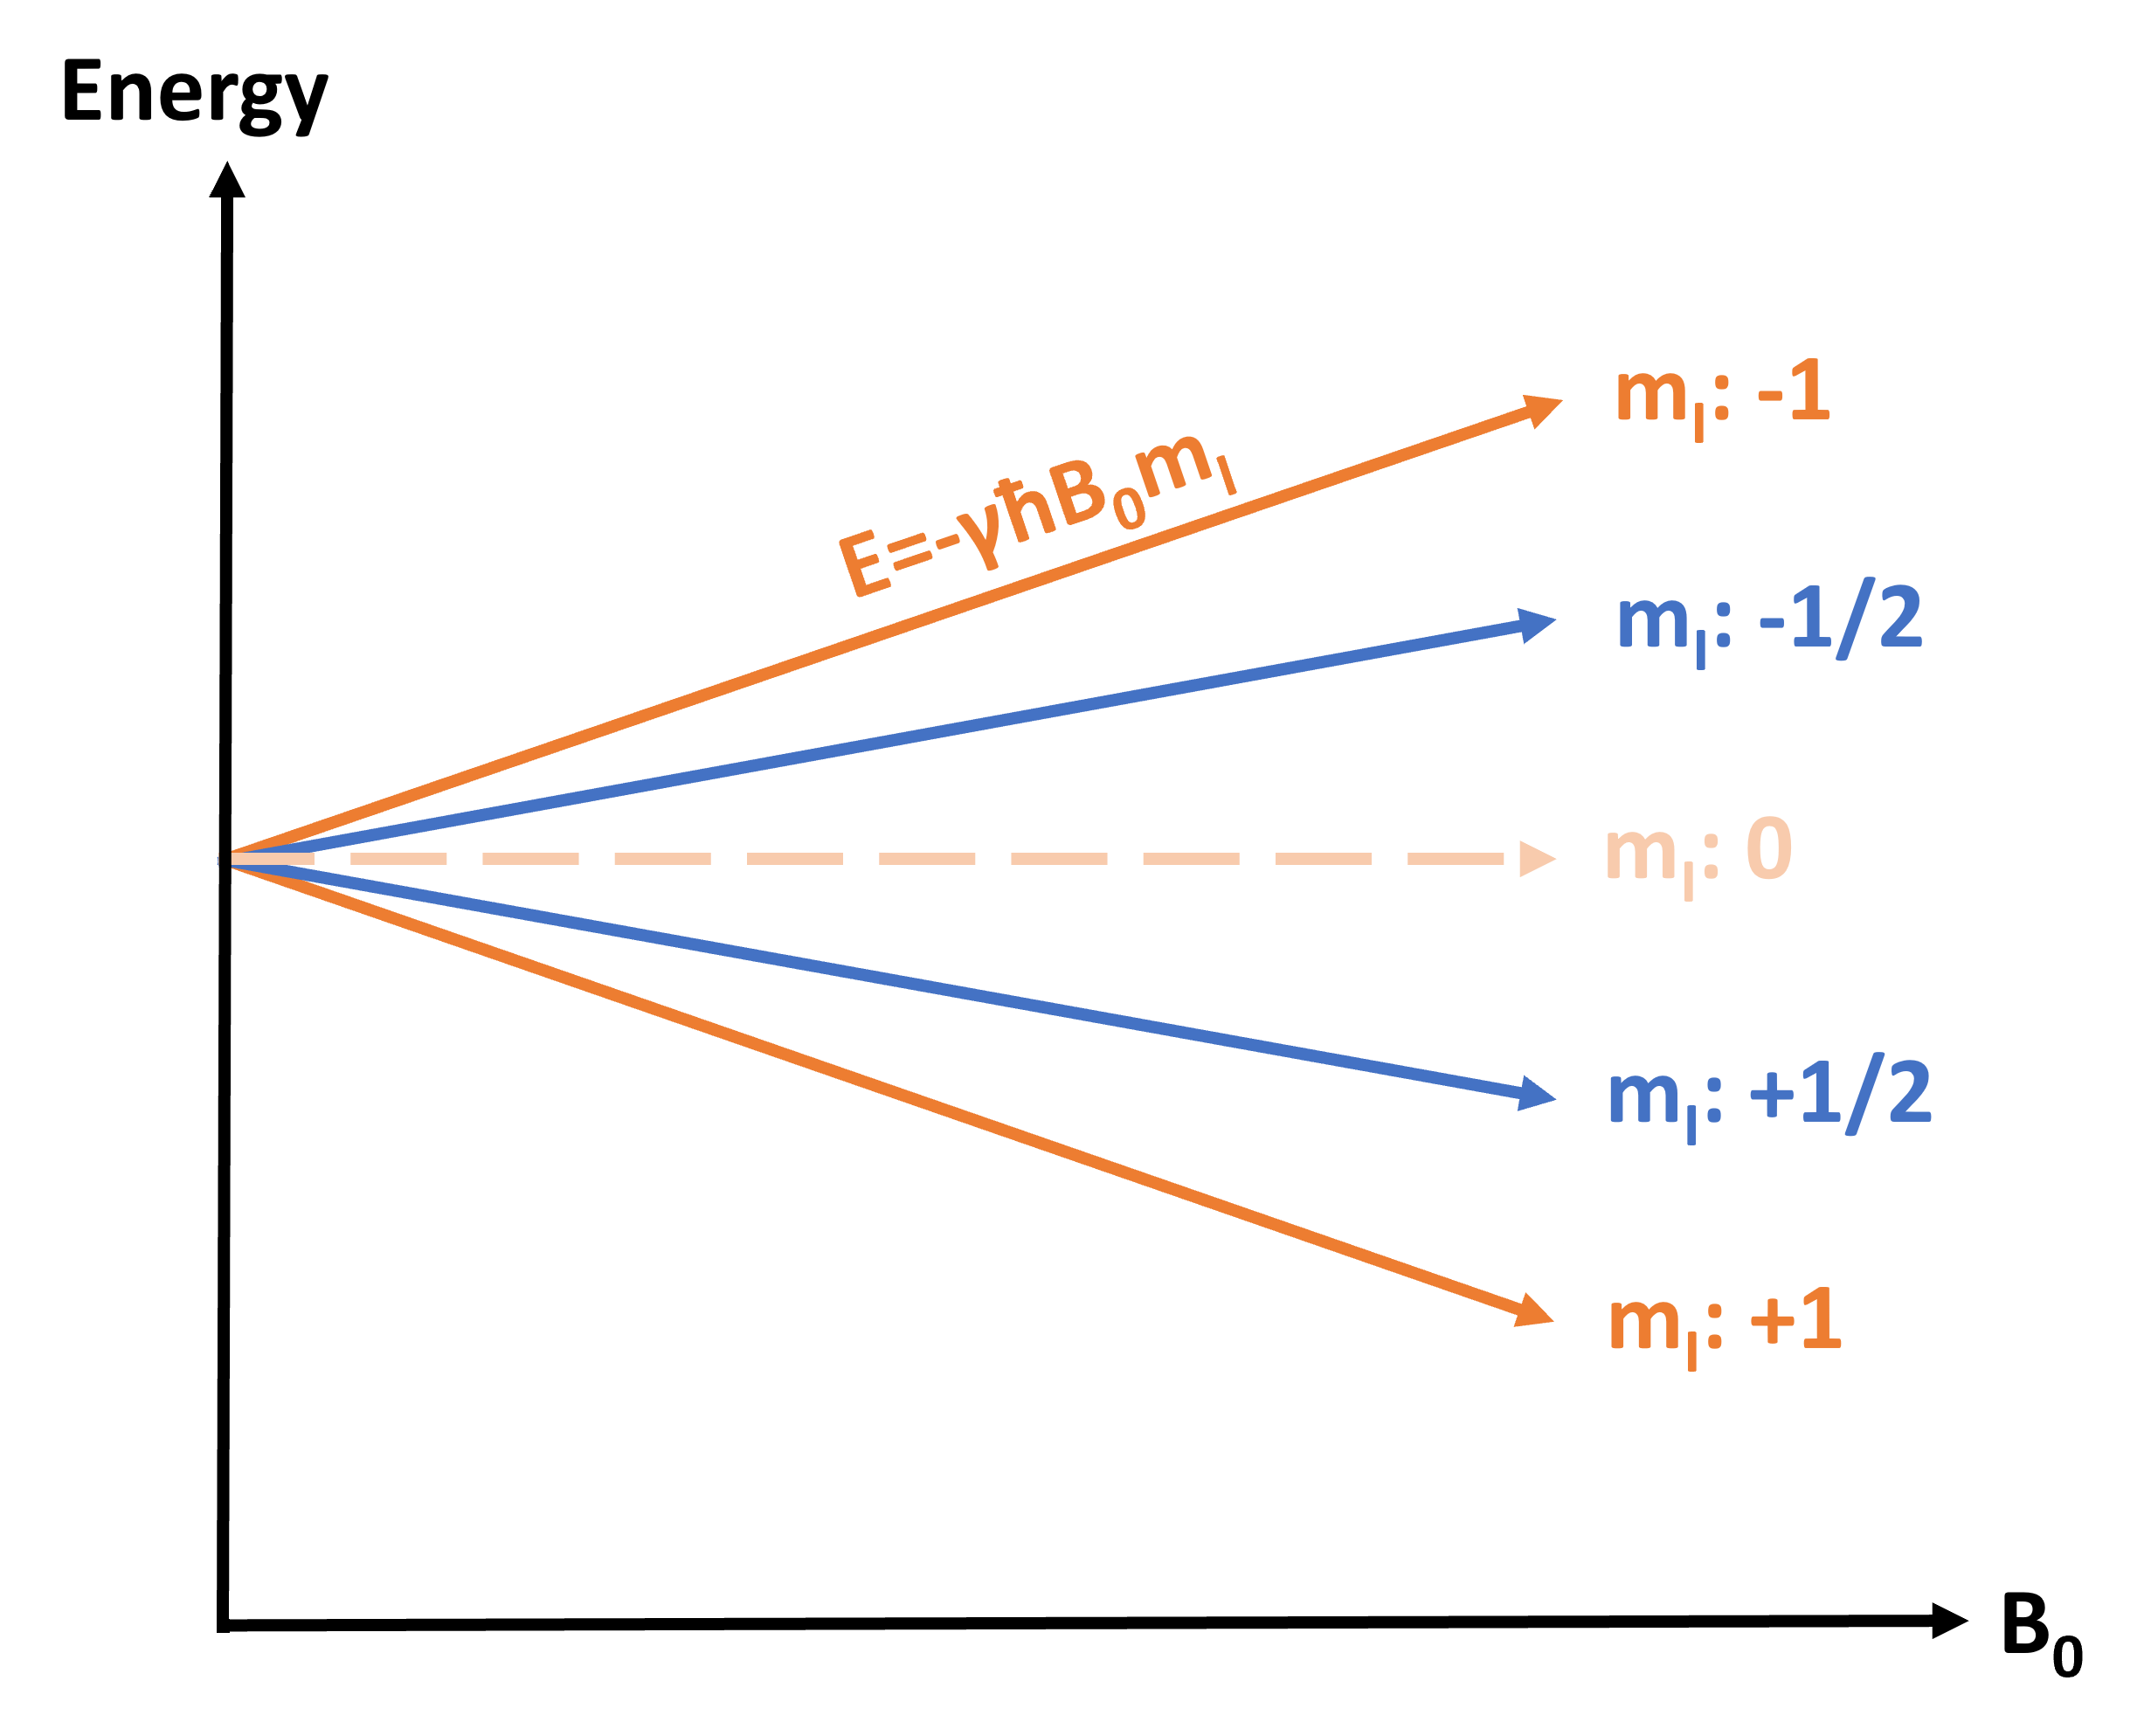
\includegraphics[width=0.8\textwidth]{Figures/Theory/Zeeman.png}
    \caption{\textit{Figure demonstrating the change in spin energy levels due to increasing magnetic field B$_0$, for spin-1/2 and spin-1 nuclei. Demonstrating the Zeeman Effect \cite{Zeeman1896VerslagenAfdeeling}.}}
    \label{fig:theory:zeeman}
\end{figure}

This gives a good overview of how individual spins act and behave in magnetic fields, however our bodies contain a collection of spins of different nuclei. Therefore, it is important to apply these relationships to a collection of spins which will give an overview of macroscopic behaviours that make up the theory of \ac{NMR}.

\subsection{Macroscopic Behaviour}

The molecules of interest for \ac{MRI} are in the liquid state which means the motion of the spin is largely random and due to Brownian motion, thermal energy then becomes the dominant driving force and therefore quantum effects become negligible. When particles have a large enough temperature ($T$) and there are enough particles, the distribution over multiple energy levels can be described according to the Boltzmann distribution \cite{Boltzmann1872WeitereGasmolekulen}. Equation \ref{eqn:theory:boltz} states the probability $p$ of a single particle being in a specific state.

\begin{equation}
    p_i = \frac{\exp\left(\frac{-E_i}{k_BT}\right)}{\displaystyle \sum_{j = 1}^{M}\exp\left(\frac{-E_j}{k_BT}\right)}
    \label{eqn:theory:boltz}
\end{equation}

\noindent where $i$ indicates the specific energy level and $M$ is the total number of available states for a specific nucleus. The overall magnetic field that results from a large group of spins can be described by a vector called the magnetisation ($M$). Most of the spins contributions will cancel so the only contribution to the magnetisation vector arises from the difference in the populations of the different energy levels. A generalised summation that calculates the equilibrium magnetisation is shown in Eq. \ref{eqn:theory:mag}.

\begin{equation}
    M = N\sum_{j = 1}^{M}p_j\mu_j
    \label{eqn:theory:mag}
\end{equation}

\noindent where $N$ is the number of spins of interest. 

A major assumption that is made to get to this point which is that the thermal energy at room temperature is much larger than the nuclear magnetic energies ($\gamma \hbar B_0\ll k_BT$). A more simplified version of Eq. \ref{eqn:theory:mag} that is still general to all spins is empirically shown in Eq. \ref{eqn:theory:mag_s}.

\begin{equation}
    M = \frac{s(s+1)\gamma^2 \hbar^2 N B_0}{3k_BT}
    \label{eqn:theory:mag_s}
\end{equation}

\noindent Most nuclei that are of interest for \ac{NMR} have a spin-1/2, which give two distinct energy levels. So in order to simplify the magnetisation calculations only the spin-1/2 nuclei are considered. Equation \ref{eqn:theory:mag_1H} calculates the equilibrium magnetisation for spin-1/2 nuclei, Eq. \ref{eqn:theory:mag_2H} calculates the equilibrium magnetisation for spin-1 nuclei such as $^2$H.

\begin{equation}
    M_0 = \frac{\gamma^2 \hbar^2 N B_0}{4k_BT}
    \label{eqn:theory:mag_1H}
\end{equation}

The equilibrium magnetisation is responsible for the signal produced in \ac{NMR} experiments. It is proportional to the total number of spins and inversely proportional to temperature (measured in kelvin). The temperature will mostly remain constant for experiments performed in humans \textit{in vivo}. Also, $M$ is proportional to the magnitude of any applied external magnetic field applied ($B_0$). The presence of equilibrium magnetisation alone is not enough for \ac{NMR}/\ac{MRI} to receive vital \textit{in vivo} information about the human body it is important to manipulate the magnetisation \cite{Haacke2014MagneticDesign}. 

\subsection{Manipulating Magnetisation}

\begin{figure}
    \centering
    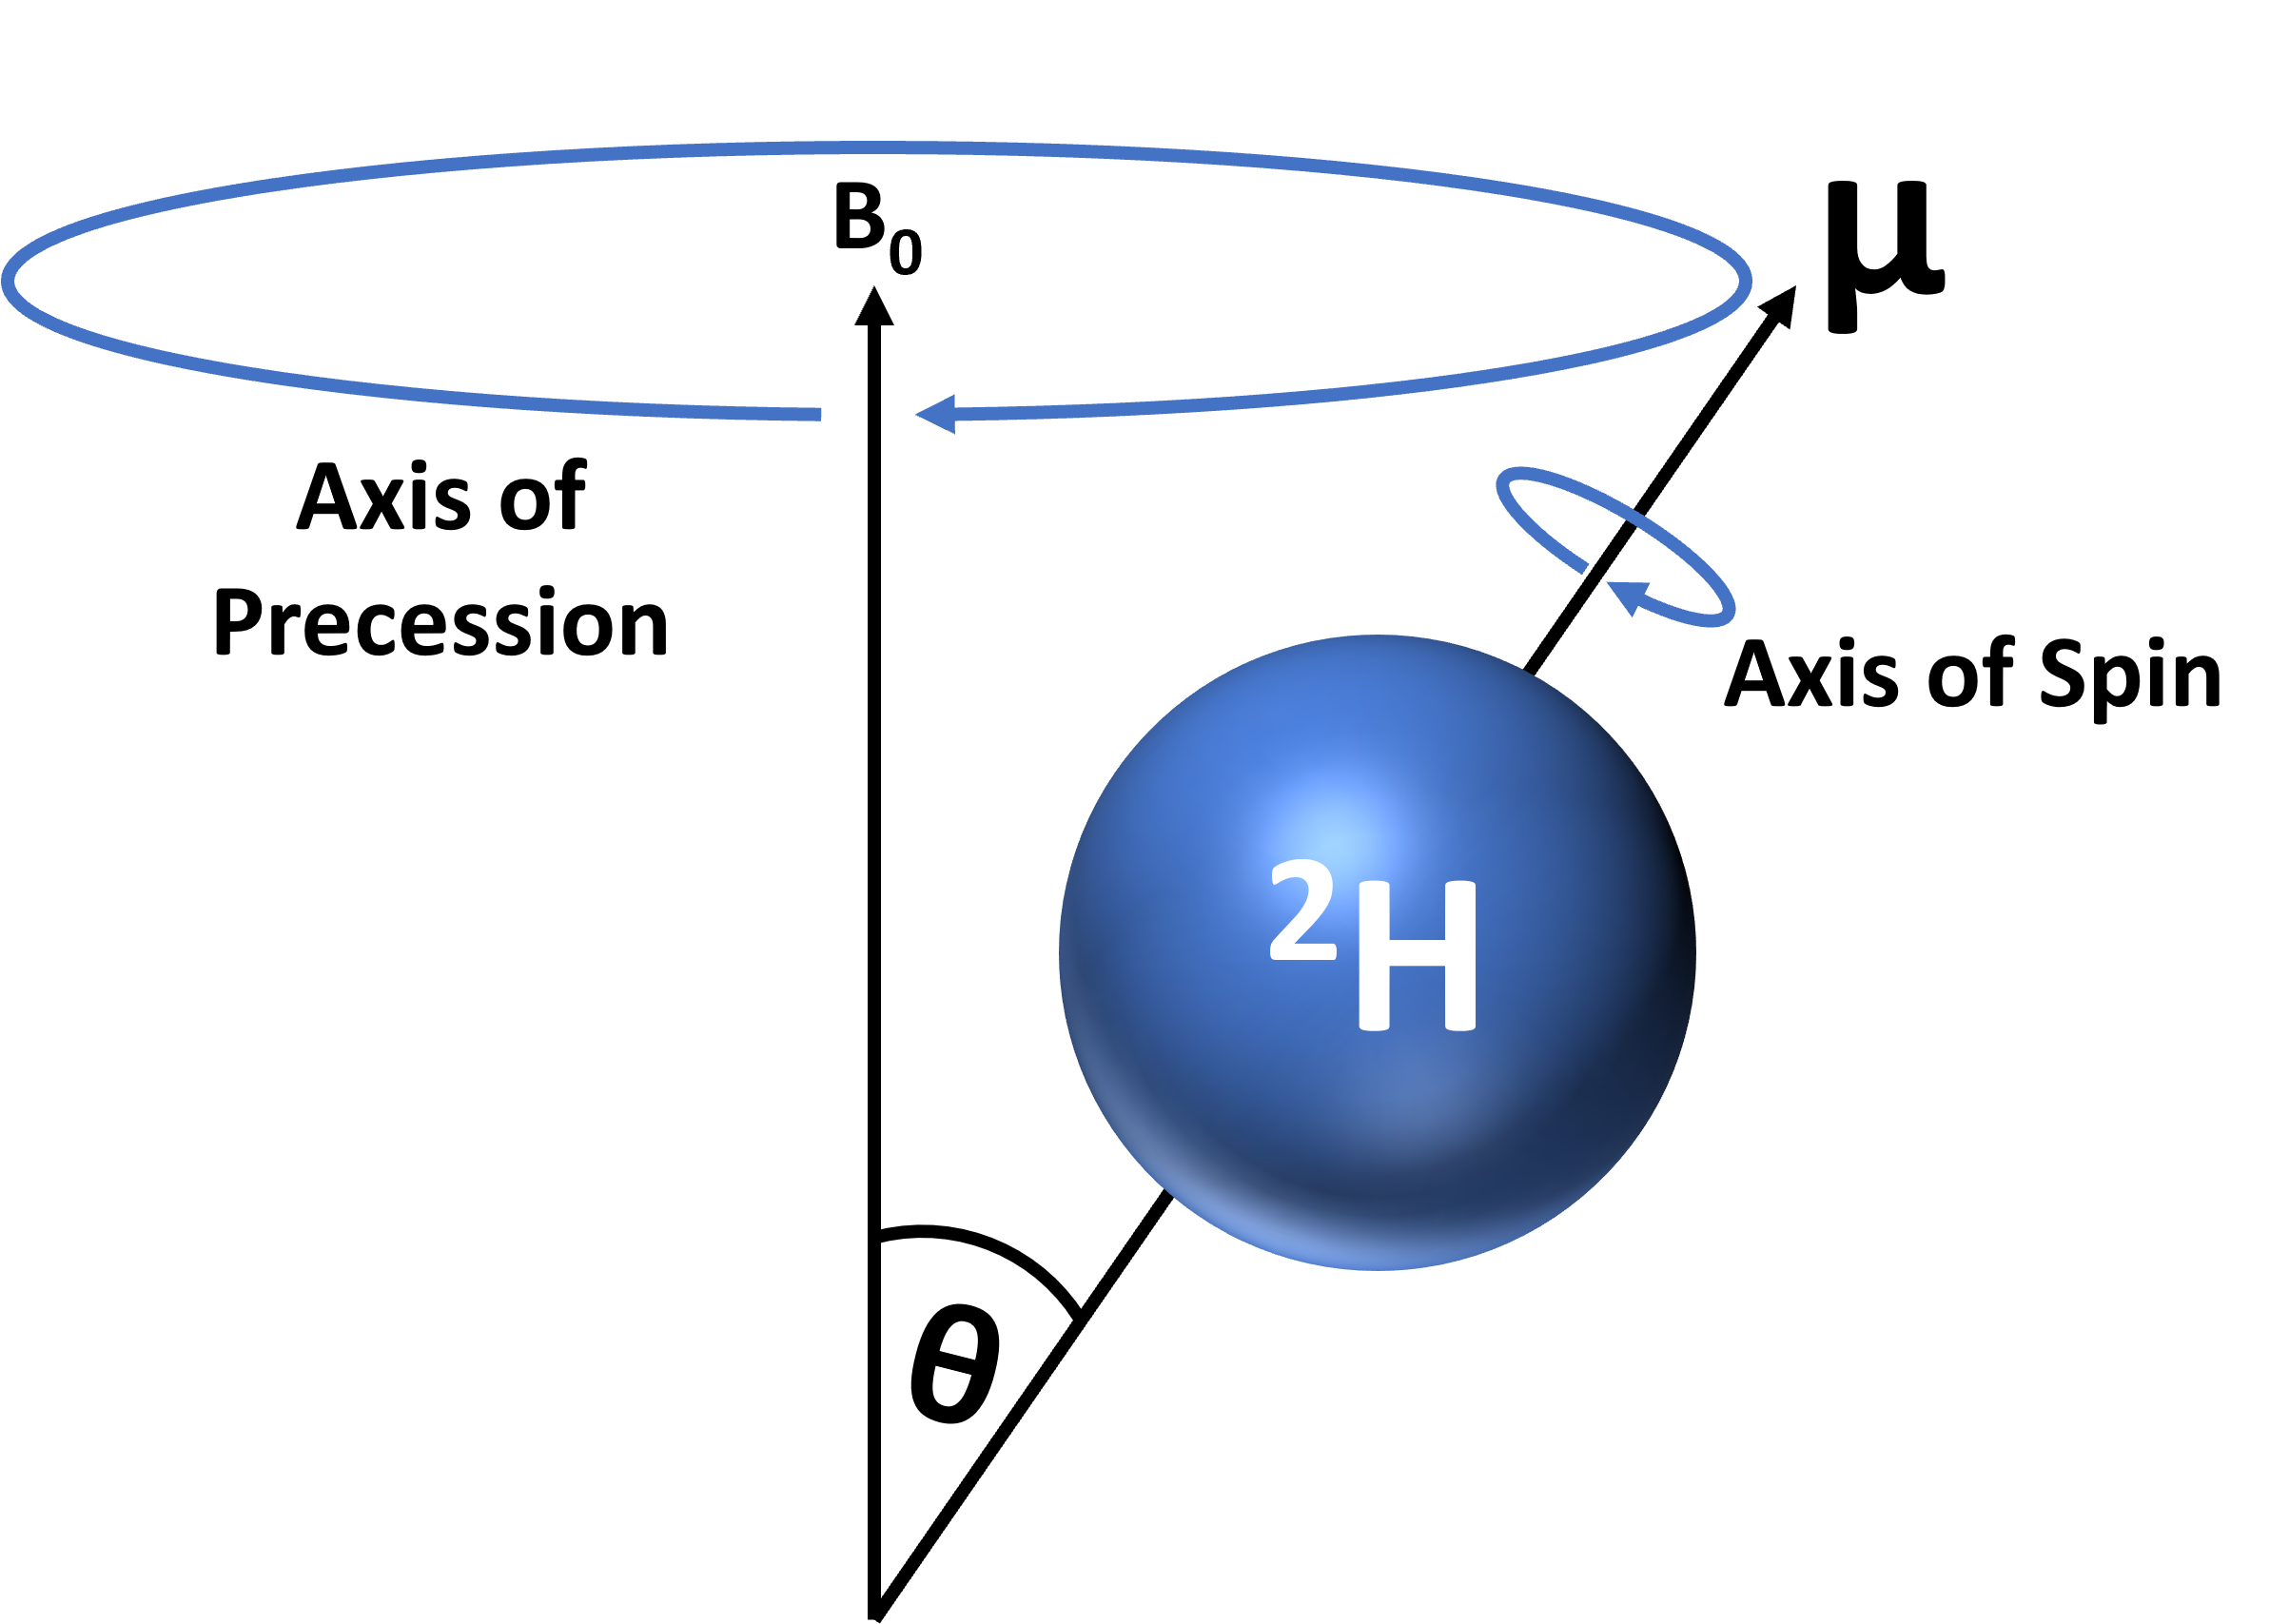
\includegraphics[width=0.9\textwidth]{Figures/Theory/Moment.png}
    \caption{\textit{A diagram of a $^2$H nuclei spinning and precessing around an applied external magnetic field B$_0$, its magnetic moment $\mu$ and both axis are labelled along with the angle the magnetic moment vector makes to B$_0$.}}
    \label{fig:theory:moment}
\end{figure}

The direction of the equilibrium magnetisation vector is the same as the applied field. In general magnetisation is made up of two main components, the longitudinal and the transverse. The longitudinal component is parallel to the applied field, with the transverse component being a combination of the two other orthogonal directions. Often the applied field, and analogously the magnetisation, is defined as $\mathbf{B}=B_0\mathbf{z}$ and therefore the longitudinal component is in the z-direction, which makes the transverse component a combination of the x and y components. The transverse magnetisation (M$_{xy}$) is zero at equilibrium. After a large enough period of time in an applied field the longitudinal magnetisation will reach the value outlined in Eq. \ref{eqn:theory:mag_1H} (M$_0$), whilst the transverse component will remain at zero. The evolution of the longitudinal and transverse components of the magnetisation is described by the Bloch Eq. \cite{Bloch1946NuclearInduction}.

\begin{equation}
    \frac{d\mathbf{M}}{dt} = \, \gamma\mathbf{M}\textrm{x}\mathbf{B} \, + \, \frac{M_0-M_z}{T_1}\mathbf{z} \, - \, \frac{\mathbf{M_{xy}}}{T_2}
    \label{eqn:theory:Bloch}
\end{equation}

The first term in Eq. \ref{eqn:theory:Bloch} describes the evolution of the magnetisation in the presence of a magnetic field $\mathbf{B}$. The second term describes the evolution of the longitudinal magnetisation due to longitudinal relaxation, where T$_1$ is the longitudinal or spin-lattice relaxation time constant. This relaxation, results from spins interactions with the surrounding `lattice'. The final term describes how the transverse magnetisation evolves over time, where T$_2$ is the transverse or spin-spin relaxation time constant. It arises from dephasing due to each spin's interaction with neighbouring spins. 

The transverse relaxation time described here relates to the case where the field applied is perfectly homogenous. However in reality this is rarely the case. In the presence of field inhomogeneity spins dephase more rapidly and the relevant relaxation is T$_2^*$.

\begin{equation}
    \frac{1}{T_2^*} = \frac{1}{T_2} + \frac{1}{T_2^{'}}
    \label{eqn:theory:trans}
\end{equation}

Here T$_2^{'}$ is dependent only on the homogeneity of the field. This means that T$_2^*$ can change between scans and scanners ect. Realistically T$_2^*$ does not vary much between cases. The relaxation times T$_1$ and T$_2^*$ are specific for each nuclei, tissue type and field strength. In spectroscopy the \ac{FWHM} of each signal/peak is related to the total transverse relaxation (\ac{FWHM}$ = 1 / \pi T_2^*$). 

%The Bloch equation can then be separated for each component ($x,y,z$) and made specific for each experiment, for example there is the static field case substituting $\mathbf{B}=B_0\mathbf{z}$, or it is possible to flip the magnetisation into the transverse plane using $\mathbf{B}=B_0\mathbf{z}+B_1\mathbf{x}$. 

\begin{figure}
    \centering
    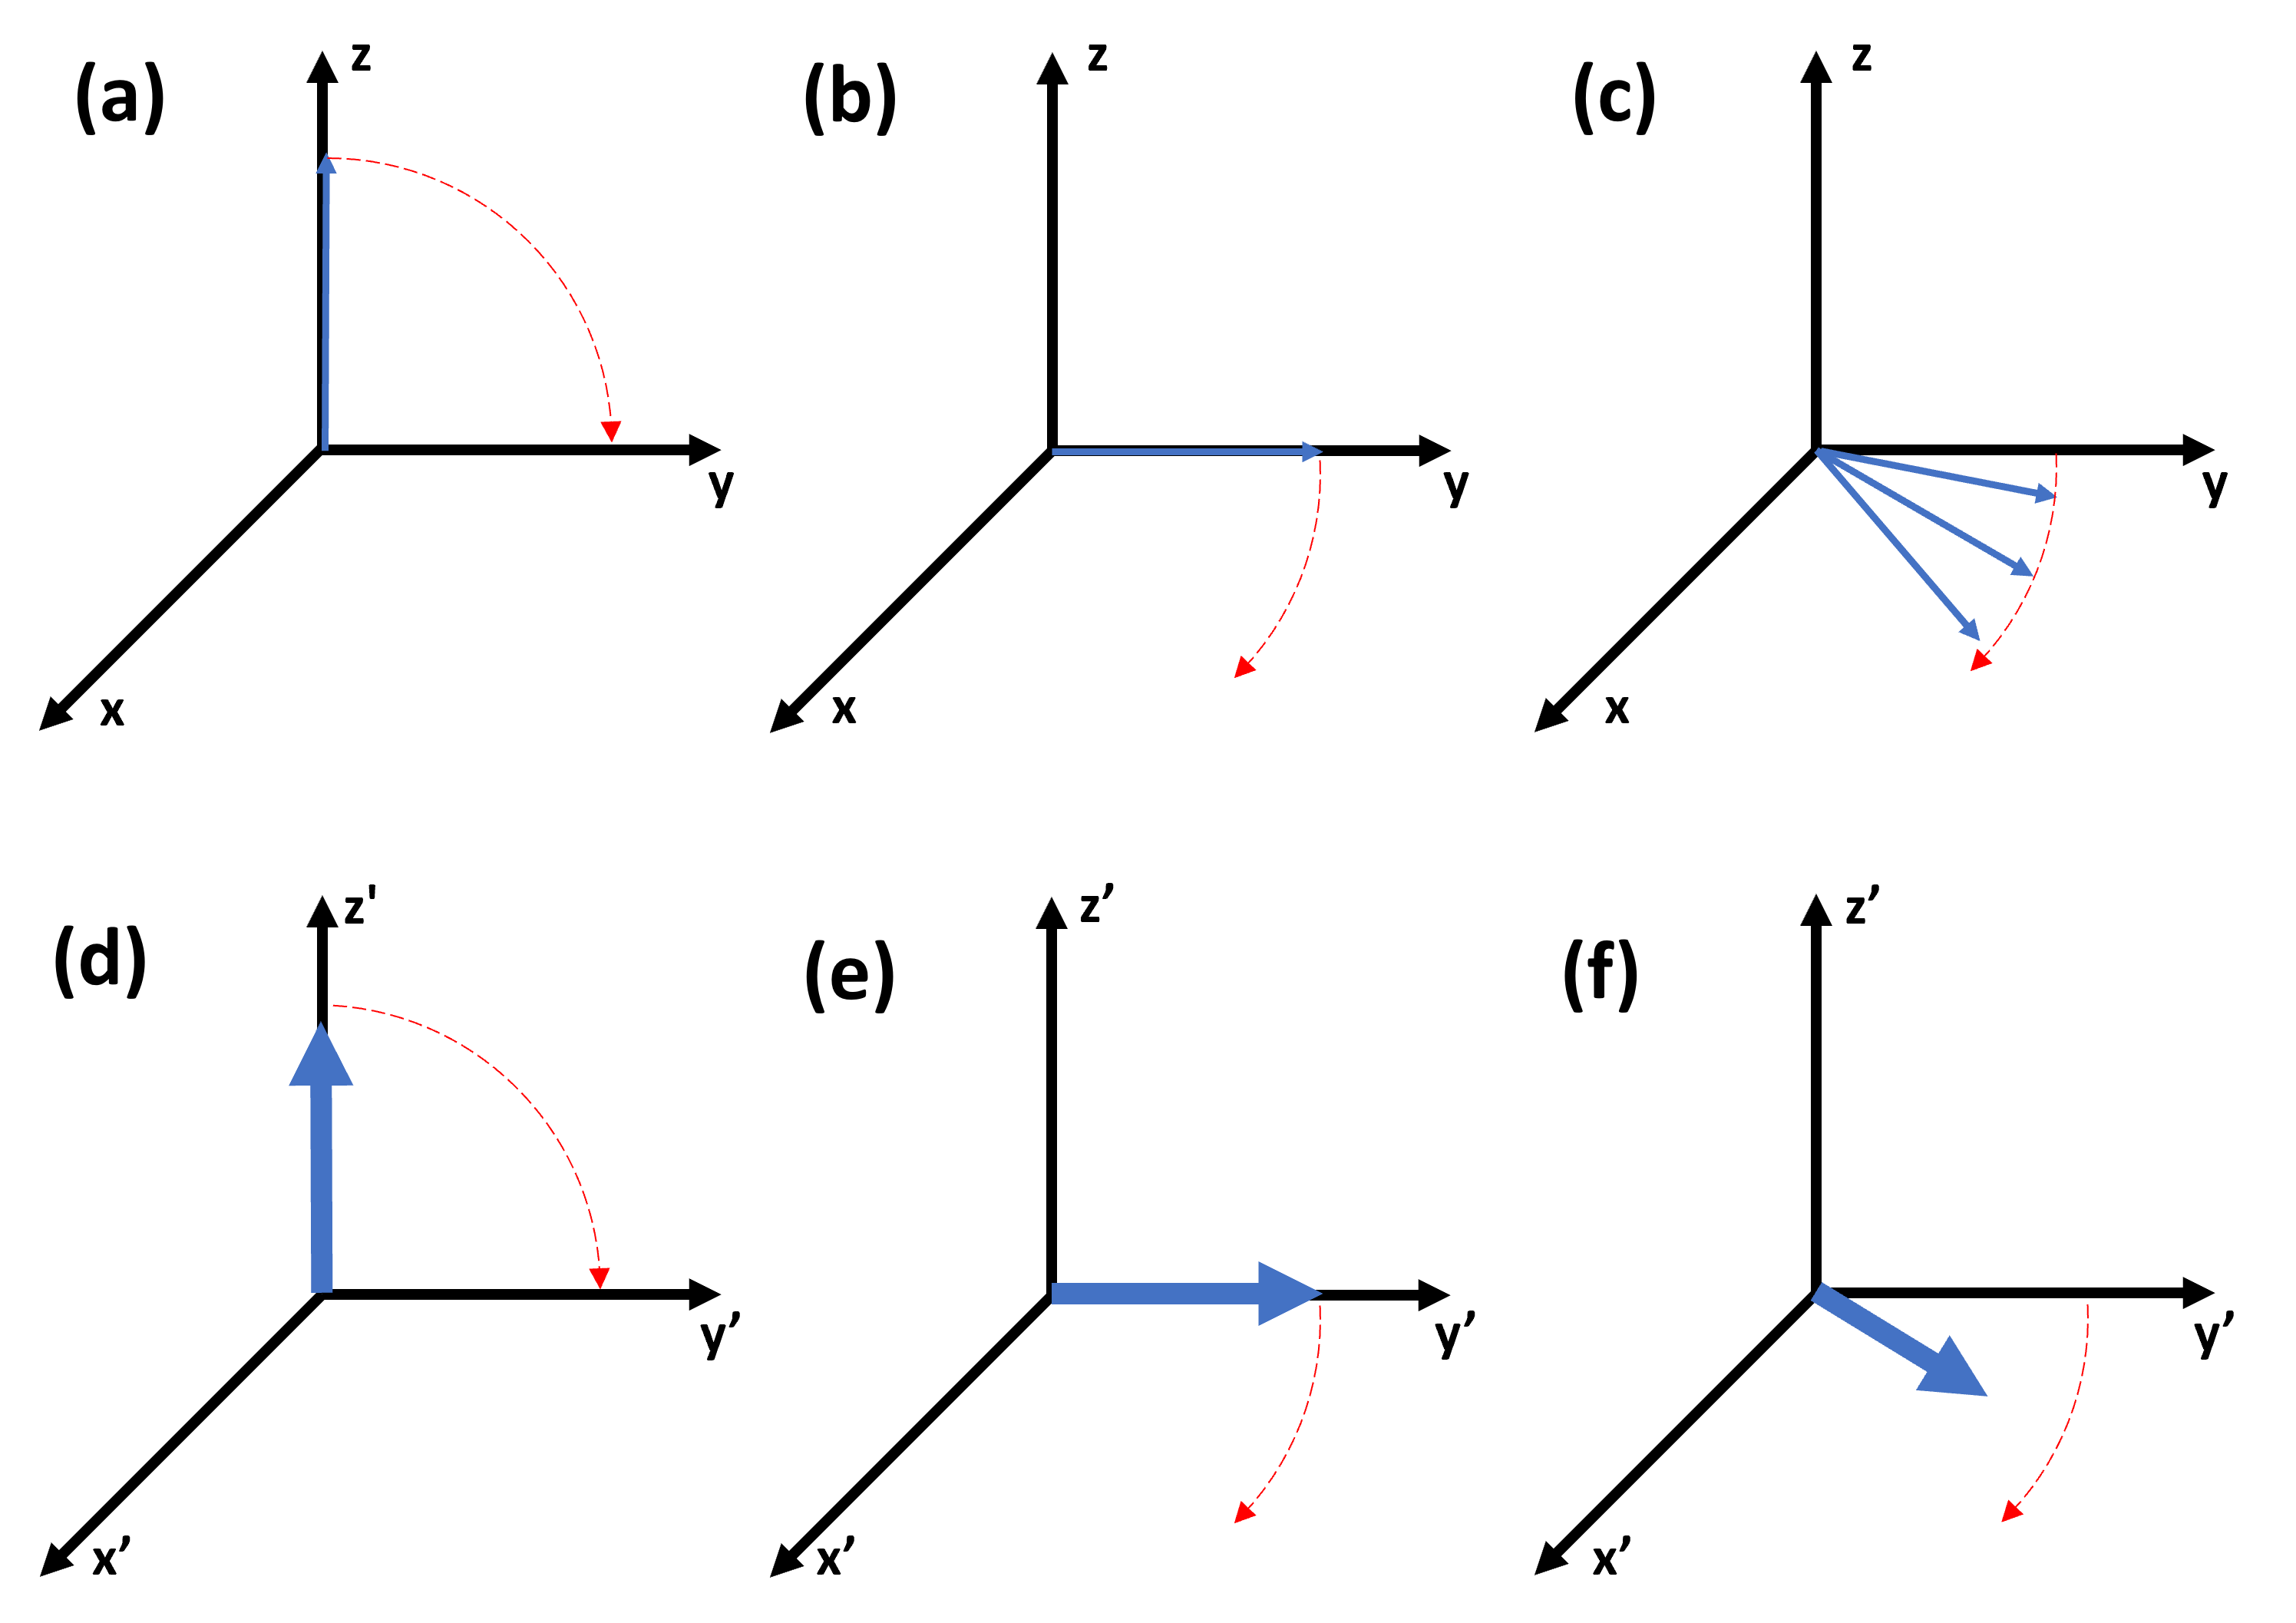
\includegraphics[width=0.9\textwidth]{Figures/Theory/Magnetisation.png}
    \caption{\textit{Diagram visually showing the effect of applied external magnetic fields on magnetic moment vectors and magnetisation.(a) Shows the precession of a collection of magnetic moment vectors after a static magnetic field (B$_0$) is applied the z-direction, and just before a 90$^\circ$ degree pulse (B$_1$) is applied. (b) Here the magnetic moments have been tipped to all align in the positive y-direction following an applied 90$^\circ$ \ac{RF} with $B_1$ along $x$ in the rotating frame. (c) After the \ac{RF} pulse the spins begin to dephase , with the spins `fanning' out in the x-y plane until no overall transverse magnetisation is left. (d-f) Show the spins experiencing the same B$_0$ and B$_1$ as in (a-c) except now only the overall magnetisation vector is shown in the rotating reference frame.}}
    \label{fig:theory:Mag}
\end{figure}


The \ac{NMR} signal arises from the longitudinal magnetisation, however this is very small and can be dominated by magnetisation from electron currents within atoms and molecules. Therefore the magnetisation is often tipped into the transverse plane where it is in the same plane as the precession and will therefore induce current in a receiver coil, at the Larmor frequency. This is achieved by applying a short alternating magnetic field $\mathbf{B} = B_1\hat{x}\cos (\omega t)$, this is often referred to as an \ac{RF} pulse since the frequency is in the \ac{RF} range.

The precession of magnetisation can be difficult to conceptualise/visualise in a stationary reference frame due to the complex 3D motion. Therefore it is beneficial to consider the system in a rotating frame of reference ie. as if the observer rotates around the z-axis. The common reference frame used is one that rotates at the frequency of the applied \ac{RF} around the z-axis, this is because the \ac{RF} pulse is made up of 2 counter-rotating components one of which will appear as stationary in the rotating reference frame. This gives the following separated Bloch equations for the evolution of magnetization ($x',y',z$) in the rotating reference frame, for a left-circularly polarised \ac{RF} field B$_1$ which is assumed to be parallel to $x'$ in the rotating frame.

\begin{equation}
    \frac{dM_{x'}}{dt} = \Delta\omega M_y^{'} - \frac{M_x^{'}}{T_2}
    \label{eqn:theory:Blochx}
\end{equation}
\begin{equation}
    \frac{dM_{y'}}{dt} = \Delta\omega M_x^{'} + \omega_1M_z^{'} - \frac{M_y^{'}}{T_2}
    \label{eqn:theory:Blochy}
\end{equation}
\begin{equation}
    \frac{dM_z}{dt} = -\omega_1M_y^{'} + \frac{M_0-M_z^{'}}{T_1}
    \label{eqn:theory:Blochz}
\end{equation}

Here, $\Delta\omega$ is the difference between the Larmor frequency ($\omega_0$) and the frequency of the rotating reference frame ($\omega$), and represents any off resonance effects and $\omega_1=\gamma B_1$. Therefore, if the \ac{RF} is applied at the Larmor frequency, these terms disappear. If only the static field case is being considered, the $\omega_1$ terms disappear as well, which leaves only the relaxation dominant terms. If short-lived \ac{RF} pulses are considered the solutions to Eqs. \ref{eqn:theory:Blochx} - \ref{eqn:theory:Blochz} describing the evolution of magnetisation of that are after the pulse are shown in Eqs. \ref{eqn:theory:xprime} - \ref{eqn:theory:zprime}.

\begin{equation}
    M_{x'}(t) = \exp(-t/T_2) \left( M_{x'}(0)\cos\Delta\omega t \, + \, M_{y'}(0)\sin\Delta\omega t \right)
    \label{eqn:theory:xprime}
\end{equation}
\begin{equation}
    M_{y'}(t) = \exp(-t/T_2) \left( M_{y'}(0)\cos\Delta\omega t \, - \, M_{x'}(0)\sin\Delta\omega t \right)
\end{equation}
\begin{equation}
    M_z(t) = M_z(0)\exp(-t/T_1) \, + \, M_0 \left( 1-\exp(-t/T_1) \right)
    \label{eqn:theory:zprime}
\end{equation}

RF pulses are used to rotate the longitudinal magnetisation into the transverse plane. In between short applied fields (\ac{RF} pulses) it is therefore important to wait a large enough period of time for the transverse signal to relax back into its longitudinal state before repeating the process to acquire more data. Therefore, whilst the longitudinal magnetisation is important for overall signal it is important to accurately and reliably tip the magnetisation exactly at 90$^\circ$, as deviations in this 'flip-angle' ($\theta$) could reduce the available signal \cite{deGraaf2019InSpectroscopy}.

\subsection{Flip Angles, Phase and Signal}

The flip angle ($\theta$) generated from a short, finite \ac{RF} pulse applied (excitation) is dependent on the B$_1$ magnetic field and the pulse duration ($\tau$) according \ref{eqn:theory:FA}.

\begin{equation}
    \Delta\theta = \gamma B_1 \tau
    \label{eqn:theory:FA}
\end{equation}

Where $\theta$ is the angle the magnetisation is rotated through after excitation, also known as the flip-angle.if starting from the equilibrium situation the closer this is to 90$^\circ$ the larger the amount of longitudinal magnetisation that is rotated into the transverse plane. The signal produced by precessing transverse magnetisation can be described as a complex signal such that $f(t) = R(t) + I(t)$. This is known as a \ac{FID}. The signal induced in the receiver coil after a 90$^\circ$ pulse is applied to equilibrium magnetisation can be written as.

\begin{equation}
    R(t) = M_0\cos(\omega t+ \phi)\exp(-t/T_2^*)
    \label{eqn:theory:real}
\end{equation}
\begin{equation}
    I(t) = -M_0\sin(\omega t+ \phi)\exp(-t/T_2^*)
    \label{eqn:theory:imag}
\end{equation}

\noindent where $\phi$ is the phase of the signal and represents the angle the transverse magnetisation makes to the $x'$ axis after excitation, i.e a phase of -90$^\circ$ would be aligned parallel to the y-axis. $M_0, \, \omega, \, \phi \, \textrm{and} \, 1/T_2^*$ are parameters that were mentioned in the previous section (amplitude, frequency, phase and relaxation rate) respectively. The real and imaginary components can be combined using Euler's formula to give Eq. \ref{eqn:theory:euler}. 

\begin{equation}
    f(t) = M_0\exp(-\omega t)\exp(-t/T_2^*)\exp(i\phi)
    \label{eqn:theory:euler}
\end{equation}

This signal is described in the time-domain. To separate different frequency contributions to the signal, it is useful to transform this signal into the frequency domain, which can be done using a \ac{FT} \cite{Fourier1822TheorieChaleur}. The equation used for doing this is

\begin{figure}
    \centering
    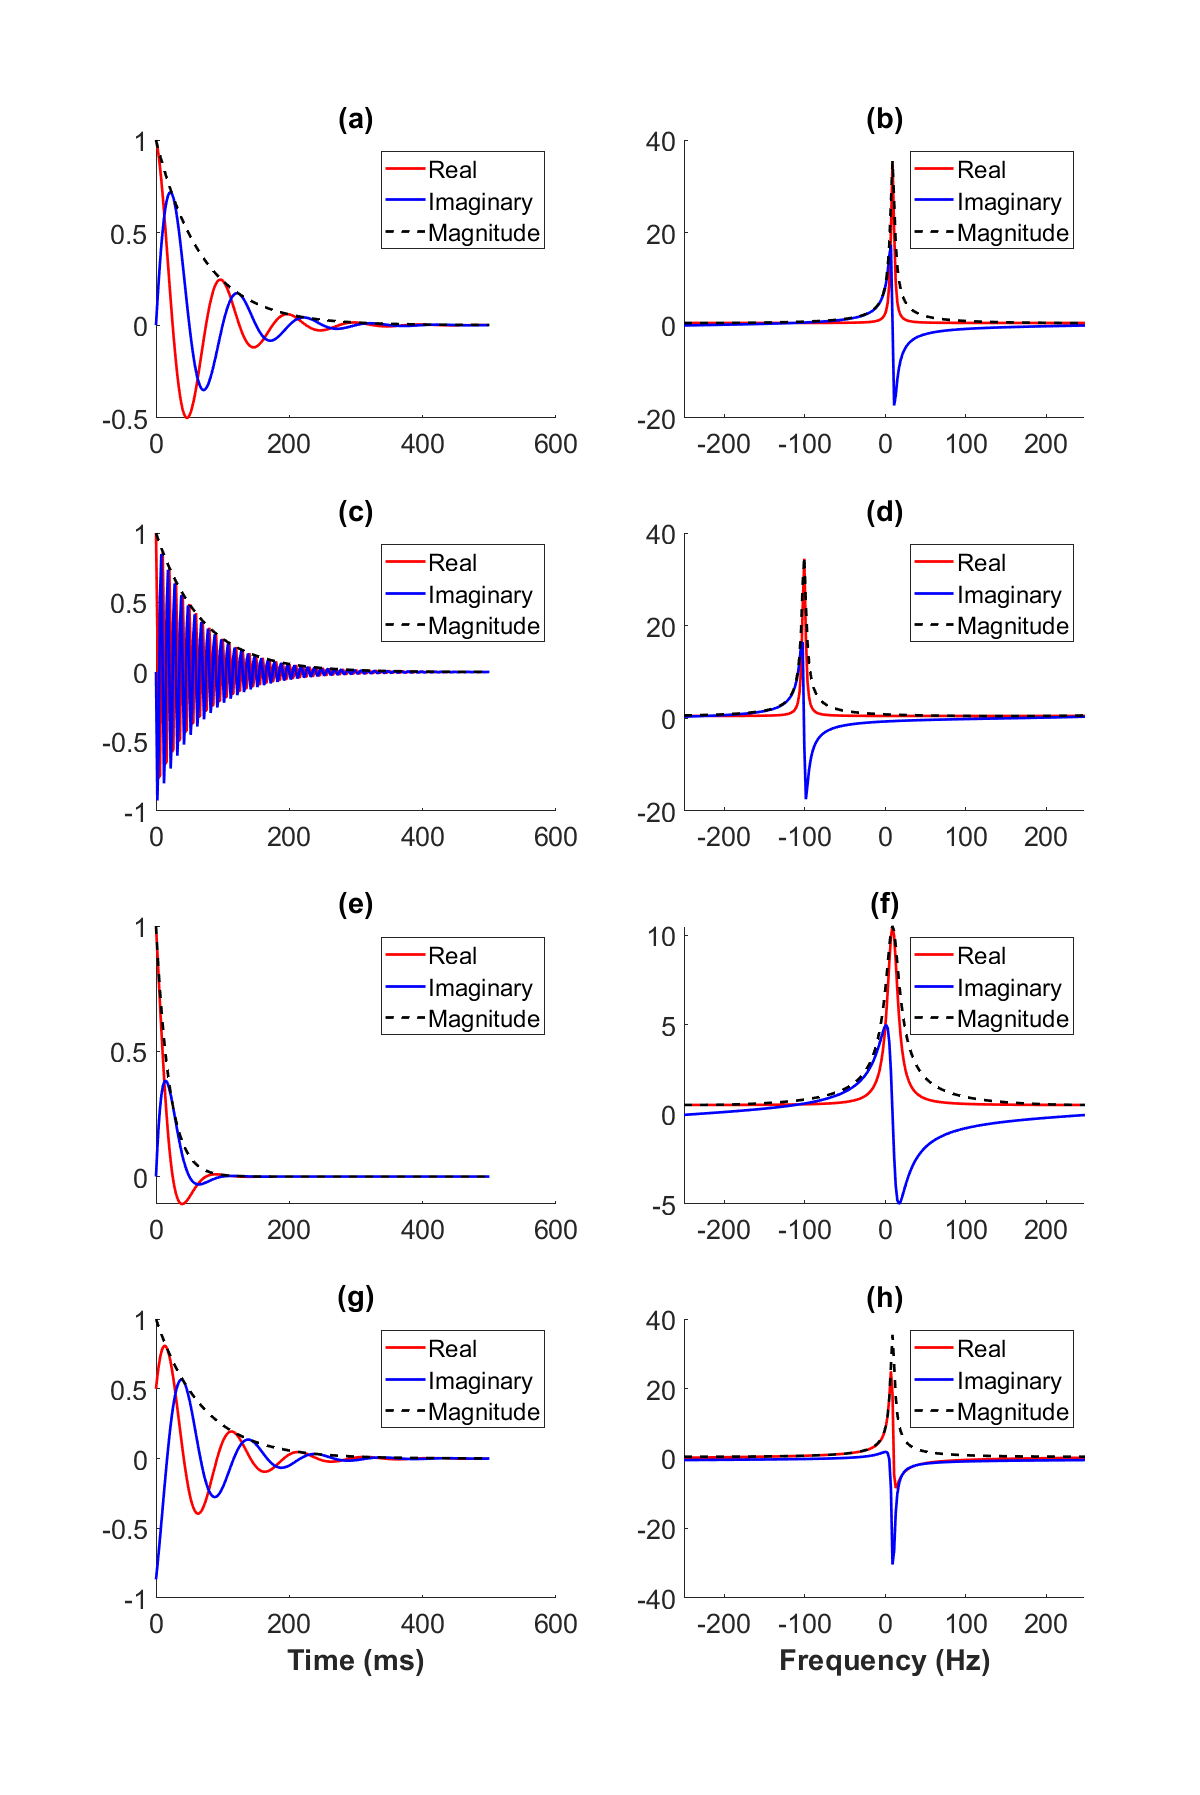
\includegraphics[width=0.9\textwidth]{Figures/Theory/FID_Lorentz.png}
    \caption{\textit{Plots of \ac{FID}s (left) and corresponding lineshapes (right) for different frequency offsets ($\nu_0$), transverse relaxation times (T$_2^*$) and phases ($\phi$), all FIDs have an amplitude ($A$) of 1. The parameters for (a) and (b) are $\nu_0$=-10 Hz, T$_2^*$= 70 ms and $\phi$=0, one parameter is changed in each row. (c) and (d) have a different $\nu_0$ of +100 Hz. (e) and (f) have a shorter T$_2^*$ of 20 ms. (g) and (h) have a phase of $\phi$=-$\pi$/3.}}
    \label{fig:theory:FID_Lorentz}
\end{figure}

\begin{equation}
    F(\omega) = \int_{-\infty}^{+\infty} f(t)\exp(-\omega t) \, dt
    \label{eqn:theory:fourier}
\end{equation}

\noindent where $F(\nu)$ is the frequency domain spectrum, $\nu$ is the frequency. By applying a \ac{FT} to the \ac{FID} Eq. \ref{eqn:theory:lorentz} is obtained, which depends on the same four parameters as the \ac{FID}. The relationship between the T$_2^*$ and the FWHM has already been shown: as the T$_2^*$ gets longer peak becomes broader. It is important to note that the integral/area under the peak is independent of T$_2^*$. The integral only depends on the amplitude (A). Therefore, the shorter the T$_2^*$ the larger the peak height and \textit{vice versa}, and therefore maximising A and minimising T$_2^*$ maximises the available \ac{SNR} in the spectrum.

\begin{equation}
    F(\nu) = A\exp(i\phi)\frac{R_2^*-i2\pi(\nu-\nu_0)}{R_2^{*2}+4\pi^2(\nu-\nu_0)^2}
    \label{eqn:theory:lorentz}
\end{equation}

Using \ac{NMR} to measure signals from pure samples with only one nuclear magnetic resonance will produce spectra with single peaks. However in general samples contain a range of different molecules, in which the atoms of each atomic species can be in different chemical environments. This is certainly the goal for \ac{MRS} measurements on living systems. The shielding of the magnetic field at the nucleus by surrounding electron cloud changes the magnetic field at the nucleus, which changes the resonant frequency of precession for nuclei. Therefore, nuclei that have different chemical environments will have different frequencies which means that the \ac{NMR} signal will be found at different frequency positions in an \ac{NMR} spectrum. Therefore by identifying the positioning of peaks in an \ac{NMR} spectra and finding the amplitudes of the peaks, it is possible to probe the chemical structure of the compounds found in the sample. This is useful in studies of medical conditions and diseases. The main unit of measure for frequency is hertz (Hz), however the values here will change greatly depending on the nuclei of interest and the field strength being used. Therefore a different unit of measurement is often used to characterise the frequency in \ac{NMR} spectra to make it more general and therefore applicable to all nuclei and field strengths. The chemical shift ($\delta$) of each signal is measured in parts-per-million (ppm). The equation to calculate chemical shift from frequency is shown in Eq. \ref{eqn:theory:chemshift}.

\begin{equation}
    \delta = \frac{\nu - \nu_{\textrm{ref}}}{\nu_\textrm{ref}} \, \textrm{x} \, 10^6
    \label{eqn:theory:chemshift}
\end{equation}

Where $\nu_{\textrm{ref}}$ is a reference frequency. So far it has been outlined how to obtain an \ac{NMR} signal in samples and in the body using MRS. However, sometimes it is not enough to just obtain information on the chemical structures/composition of the body and spatial information is also needed to interrogate chemical compositions of specific areas in the body. The most common way to do the required spatial encoding is to use magnetic fields that vary spatially \cite{Haacke2014MagneticDesign}. 

\subsection{Introduction of Gradients}

According to Eq. \ref{eqn:theory:Lamor} the frequency of precession is dependent on the applied magnetic field. Therefore if the magnetic field varies in any direction the frequency of precession will also vary in that direction. In particular a magnetic field gradient corresponding to the linear variation of field with position, produces a linear variation of frequency with position. For example when a gradient is applied in the $z$-direction.

\begin{equation}
    B = Gz,\; \omega = \gamma Gz 
\end{equation}

Previously, we considered the situation where a static spatially-homogeneous $B_0$ was applied to a sample and an \ac{RF} pulse was used to tip the magnetisation of all the spins into the transverse plane. However if a gradient is applied along with B$_0$ only the spins with the same frequency as the \ac{RF} pulse will be tipped. The magnetic field in the presence of a gradient is described by Eq. \ref{eqn:theory:B_Grad}, with the frequency that is spatially dependent is shown in Eq. \ref{eqn:theory:f_Grad}.

\begin{equation}
    B(r) = B_0 \, + \, Gr
    \label{eqn:theory:B_Grad}
\end{equation}

\begin{equation}
    \nu(r) = \frac{\gamma}{2\pi}(B_0 \, + \, Gr)
    \label{eqn:theory:f_Grad}
\end{equation}

\noindent Here $r$ is used to represent any direction. Therefore only a spatially localised 'slice' will be excited and any signal received will be specifically from that slice. By changing the frequency of the pulse applied means that a different slice can be applied. If the pulse contains a range of frequencies (bandwidth) all the frequencies in the bandwidth will be excited, this results in a slice being excited that has a physical thickness. If this process is repeated spectra can be acquired from multiple slices and therefore the changes in signals can be compared to position in the body of which the slice was acquired. The link between magnetic field/frequency and position using gradients is demonstrated visually in Fig. \ref{fig:theory:Grad}.

\begin{figure}
    \centering
    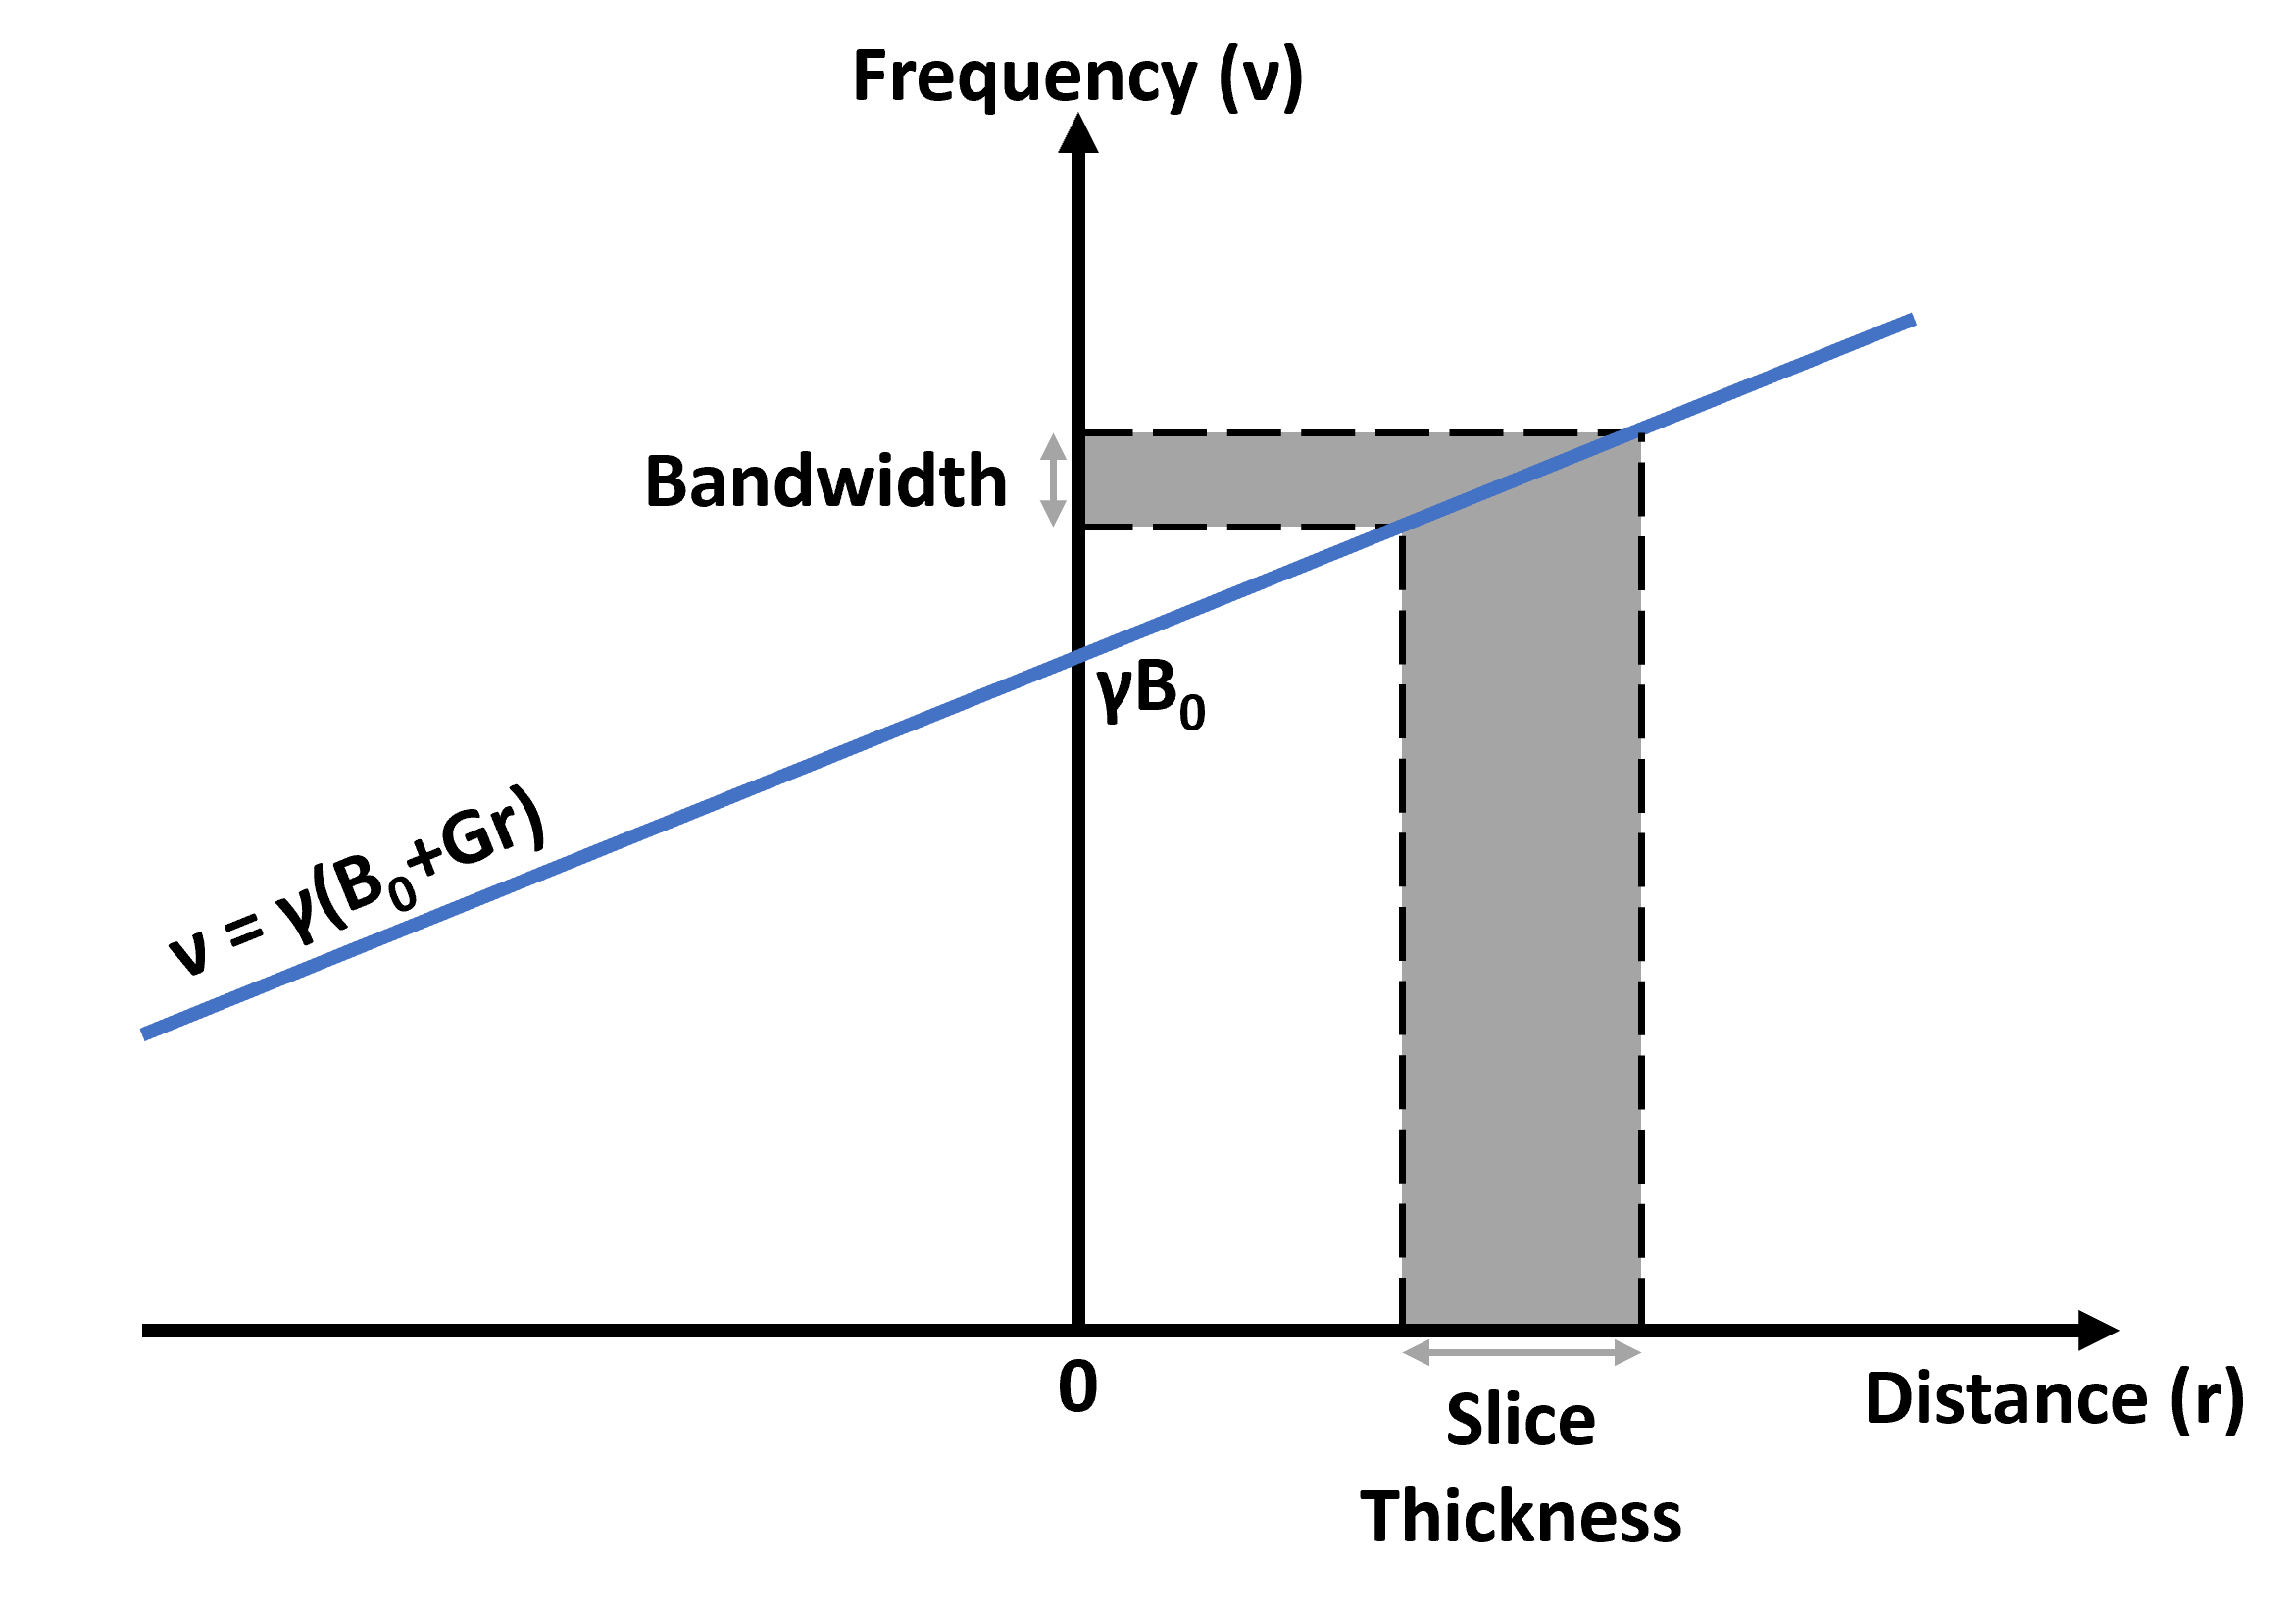
\includegraphics[width=0.9\textwidth]{Figures/Theory/Gradient.png}
    \caption{\textit{The relationship between frequency of precession ($\nu$) and thickness of an acquired slice when a gradient ($G_{slice}$) is applied.}}
    \label{fig:theory:Grad}
\end{figure}

If the chemical composition of what is being investigated is not important it is possible to acquire entirely spatial information and create a volumetric image based on multiple slices. To do this more gradients are needed than just the slice-selective gradient \cite{deGraaf2019InSpectroscopy}.

\section{Differences for $^2$H}

Deuterium ($^2$H) is a stable isotope of hydrogen. The nucleus of a $^2$H atom is called a deuteron. Large elements are formed during collisions of neutron stars \cite{Watson2019IdentificationStars}, whilst lighter elements up to iron are made in the cores of stars during fusion. However, $^2$H is destroyed very quickly in star's fusion \cite{Patrignani2016ReviewPhysics} therefore almost all the $^2$H exists naturally is formed from Big Bang Nucleosynthesis. The $^2$H abundance found in Earth's oceans is similar to what has been found in comets, which adds evidence that ocean water originates from comets \cite{Hersant2001APlanets}. Most of the natural $^2$H content occurs as \ac{HDO}, and the $^2$H content of different water sources (oceans, rainwater etc) can be used to track the water cycle \cite{Bowen2019IsotopesApplications}. Our bodies consequently have a very low \ac{NA} $\approx$0.015\% of $^2$H, which makes $^2$H appealing for tracer studies, as small concentration increases are easy to detect above baseline. The addition of a neutron to the nucleus of $^2$H means the gyromagnetic ratio ($\gamma$) is smaller than that of $^1$H (6.54 vs 42.6 MHzT$^{-1}$) which reduces the Larmor frequency of $^2$H according to Eq. \ref{eqn:theory:Lamor}. A magnetic moment is a vector quantity that is used to describe magnetic fields and interactions that arise from charges. Dipolar moments arise from dipolar charges such as point charges and bar magnets, a quadrupolar moment is a second rank expansion of the dipolar moment and is used to describe non-spherical charge distributions. $^2$H has an integer spin of 1 and due to the non-symmetric distribution of charge within the nucleus also has a quadrupolar magnetic moment of 0.286 fm$^2$. The nuclear quadrupolar moment interacts with local electric field gradients, and fluctuations in this interaction cause relaxation, thus reducing both the longitudinal and transverse relaxation times of quadrupolar nuclei. Deuterium's spin of 1 also introduces an extra Zeeman energy level more than for $^1$H, with available spin values of $m_s$ = -1, 0 and 1. Considering the magnetisation is the net vector sum of $\mathbf{\mu}$ the net magnetisation is due to the population differences between the lowest and largest energy levels. Using Eq. \ref{eqn:theory:mag} and/or \ref{eqn:theory:mag_s} a simplified equilibrium magnetisation can be found, which is shown in Eq. \ref{eqn:theory:mag_2H}.

\begin{equation}
    M_0 = \frac{2\gamma^2 \hbar^2 N B_0}{3k_BT}
    \label{eqn:theory:mag_2H}
\end{equation}

Whilst the magnetisation appears to be 8/3 larger for $^2$H compared to $^1$H in Eq. \ref{eqn:theory:mag_2H}, it is important to remind the reader that $M_0$ is also dependent on the gyromagnetic ratio squared along with the number of spins. The gyromagnetic ratio squared is $\approx$42 times smaller for $^2$H. Also assuming the mass and volume of the sample/tissue being scanned/investigated is at \ac{NA} the number of spins will be $\approx$6.7x10$^{-3}$ smaller for $^2$H. The lower value of $\gamma$ also reduces the Larmor frequency, leading to a further reduction in the NMR signal. This reduction in $\gamma$ means stronger gradients are needed to produce the same amount of spatial encoding. As a consequence some of the loss in signal of $^2$H can thankfully be recovered due to the reduction in relaxation times. This is because the signal will return to equilibrium more rapidly and therefore the scans can be more rapidly repeated and averaged, increasing the number of averages that can be acquired per unit time. The decrease in \ac{SNR} for $^2$H compared to $^1$H makes \ac{MRI} difficult at \ac{NA}, which is why spectroscopic techniques are much more common for $^2$H. 

% \subsection{Other Nuclei} Potential subsection
% Carbon-13, Phosphorous-31

\section{Scanning}   

\subsection{Imaging}

\begin{figure}[h]
    \centering
    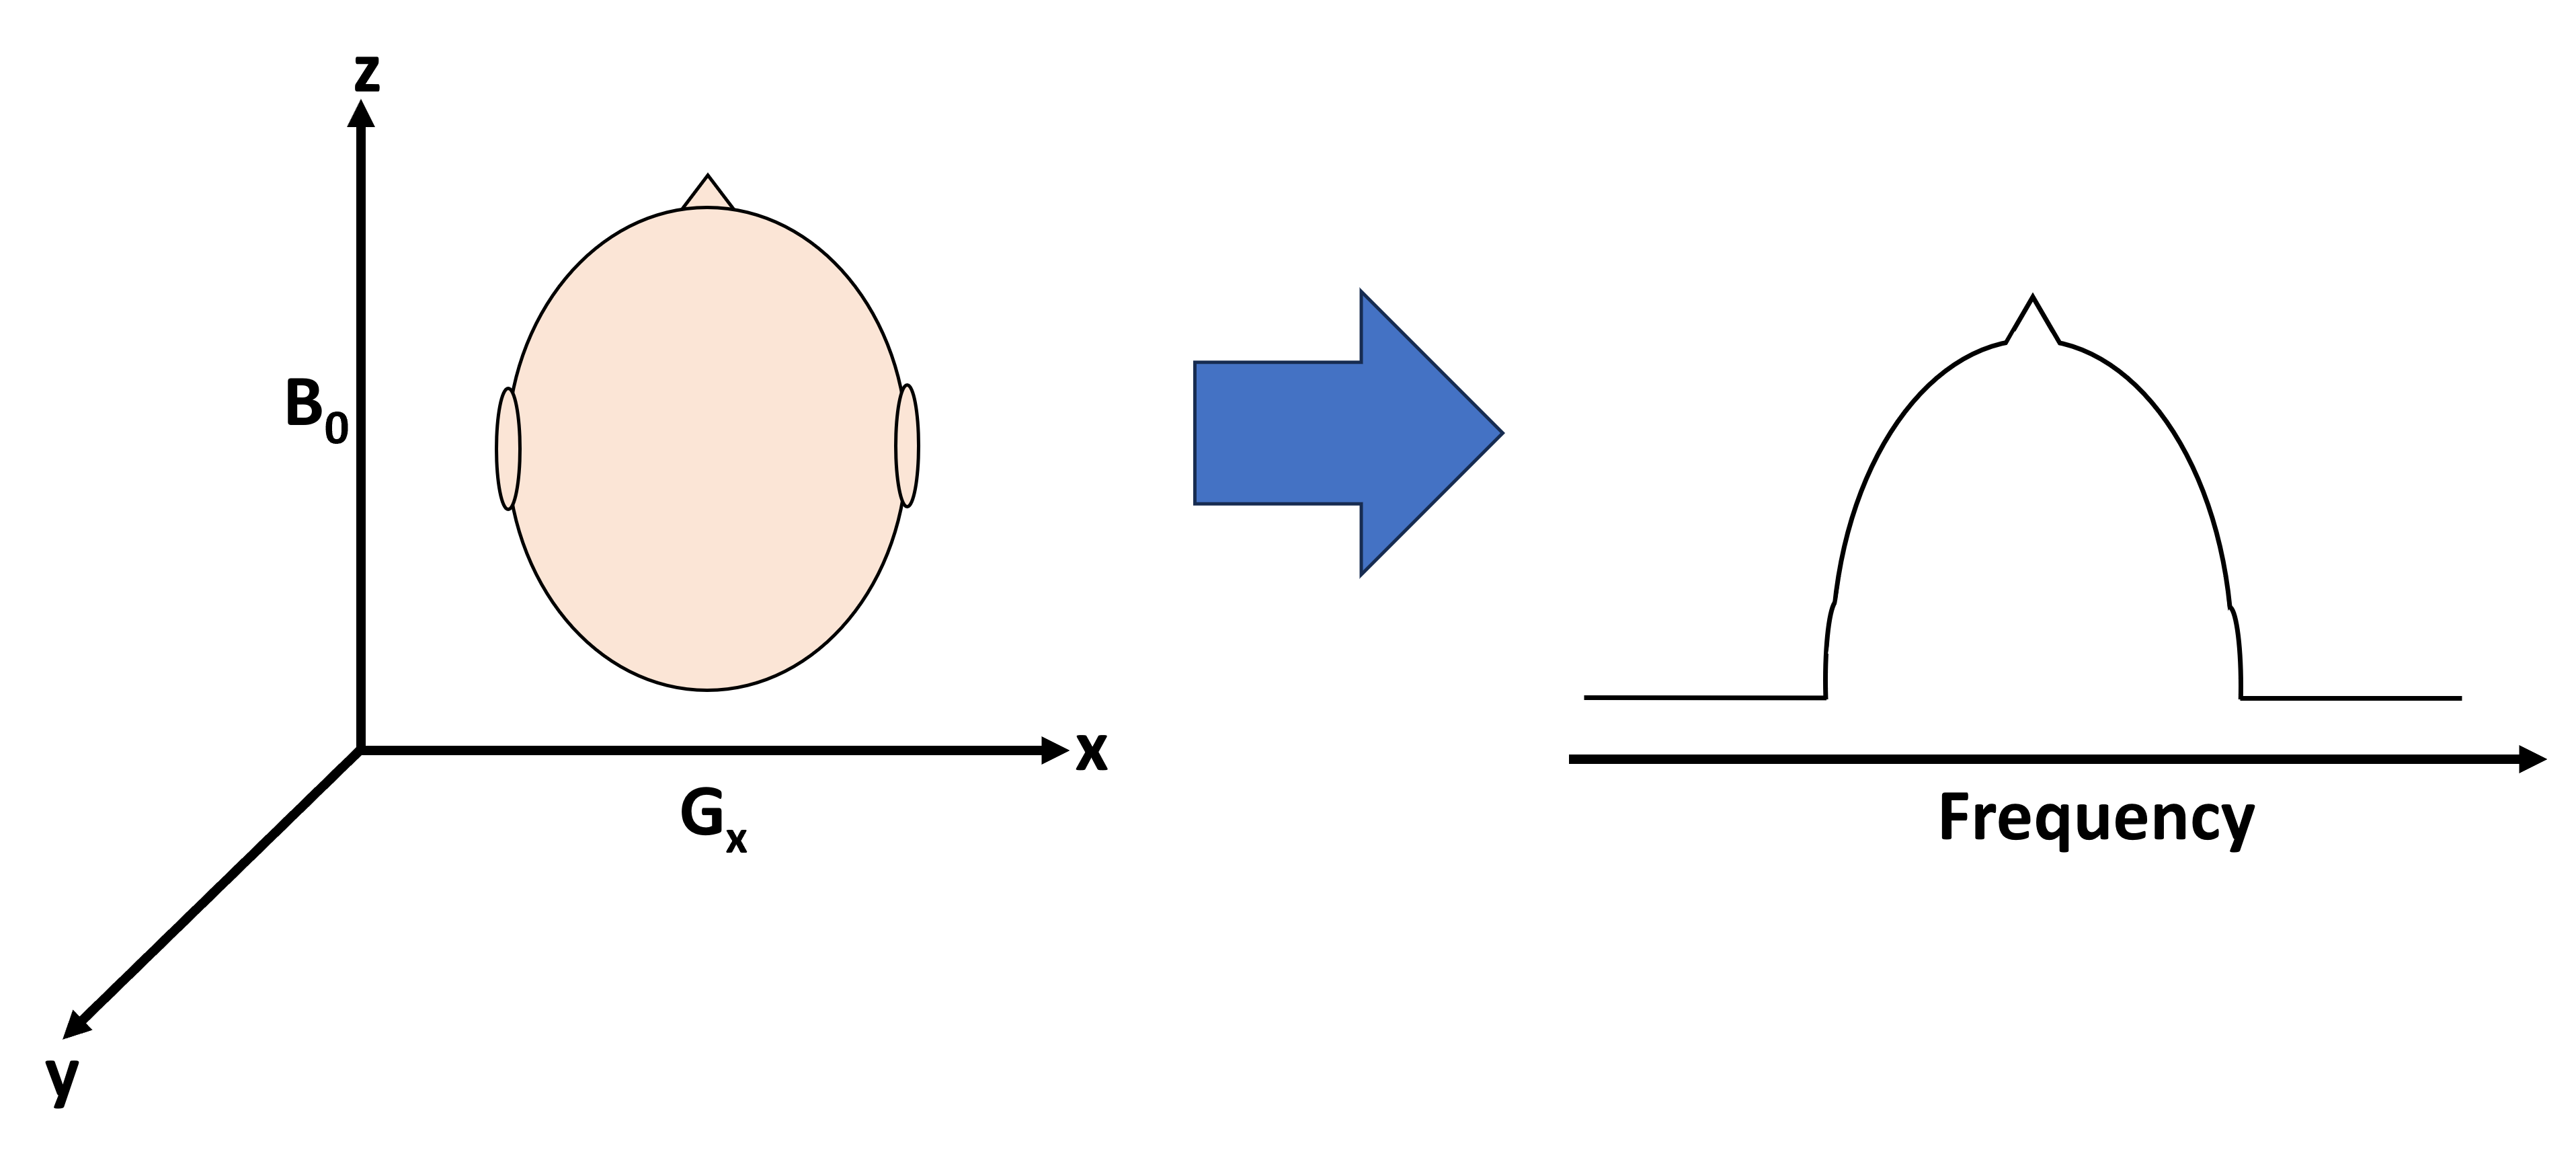
\includegraphics[width=1\textwidth]{Figures/Theory/1D_Projection.png}
    \caption{Diagram showing how a 1D projection of an image is created using a gradient applied in the x direction.}
    \label{fig:theory:1D}
\end{figure}

The use of gradients during \ac{RF} pulse excitation to excite signals selectively within a thin slice of the object, known as slice selection, is the first step in using magnetic fields to obtain images. In addition to slice selection two more directions also need to be encoded. If a gradient is applied immediately after the excitation the \ac{FID}and corresponding spectrum will contain spatial information, as the frequency shift of peaks will inform on location of the signal in a similar way to the slice selection. The spectrum then represents a 1D projection of the spin density of whatever is being scanned. The spectral width of the obtained signal therefore identifies on the width/size of the image which is often referred to as the \ac{FOV}. This method of encoding an additional dimension is known as frequency encoding using a readout/frequency gradient (G$_{\textrm{read}}$/G$_{\textrm{freq}}$), with the obtained 1D spectrum being known as the readout profile.

Whilst frequency encoding does work to obtain an additional dimension, there are real world limitations that can hinder this process. The main limitation is the gradient switching as the turning on/off of the gradient cannot occur instantaneously therefore the first few \ac{FID} points might be acquired during a time-varying gradient which will lead to errors in the data, which will persist into the spectrum after an \ac{FT} is applied. A method of getting around this is to remove first few points from the \ac{FID}, however these contain the highest signal and therefore could reduce the available \ac{SNR}. The realistic method to navigate around this problem is to create an signal at a later time point by taking advantage of dephasing and rephasing, the later signal is referred to as an echo. If the echo is created using a 180$^\circ$ pulse it is referred to as a \ac{SE}, if the echo is created by manipulating gradients it is referred to as a \ac{GE}. When a perfect \ac{FID}is created the signal starts with a phase of 0 at t=0 and as the magnetisation evolves in the transverse plane it begins to accumulate phase. Therefore by applying a negative G$_{read}$ which encourages the dephasing, followed by a positive G$_{read}$ the phase accumulation reverses in direction during the positive G$_{read}$ and reaches 0 again. Acquiring data at this point allows a full \ac{FID}to be obtained with the maximum signal occurring during the G$_{read}$, the echo occurs at a time referred to as the \ac{TE}. It is important to note that the rephasing only recovers the extra phasing caused by the negative G$_{read}$, it does not recover signal lost from T$_2$ or T$_2^*$ relaxation processes. Another type of echo formation exists called \ac{SE} or Hahn-echo \cite{Hahn1950SpinEchoes} which applies a 180$^\circ$ after the first set of gradients to rephase the signal, the use of \ac{GE} are often preferred to SE in terms of imaging thanks to the the lower flip angles, shorter \ac{TE} and shorter \ac{TR} that can be achieved. The \ac{TR} is the time from the end of the \ac{RF} pulse until the scan can be repeated. Repeating/averaging the scan allows the \ac{SNR} to be improved.

\begin{figure}
    \centering
    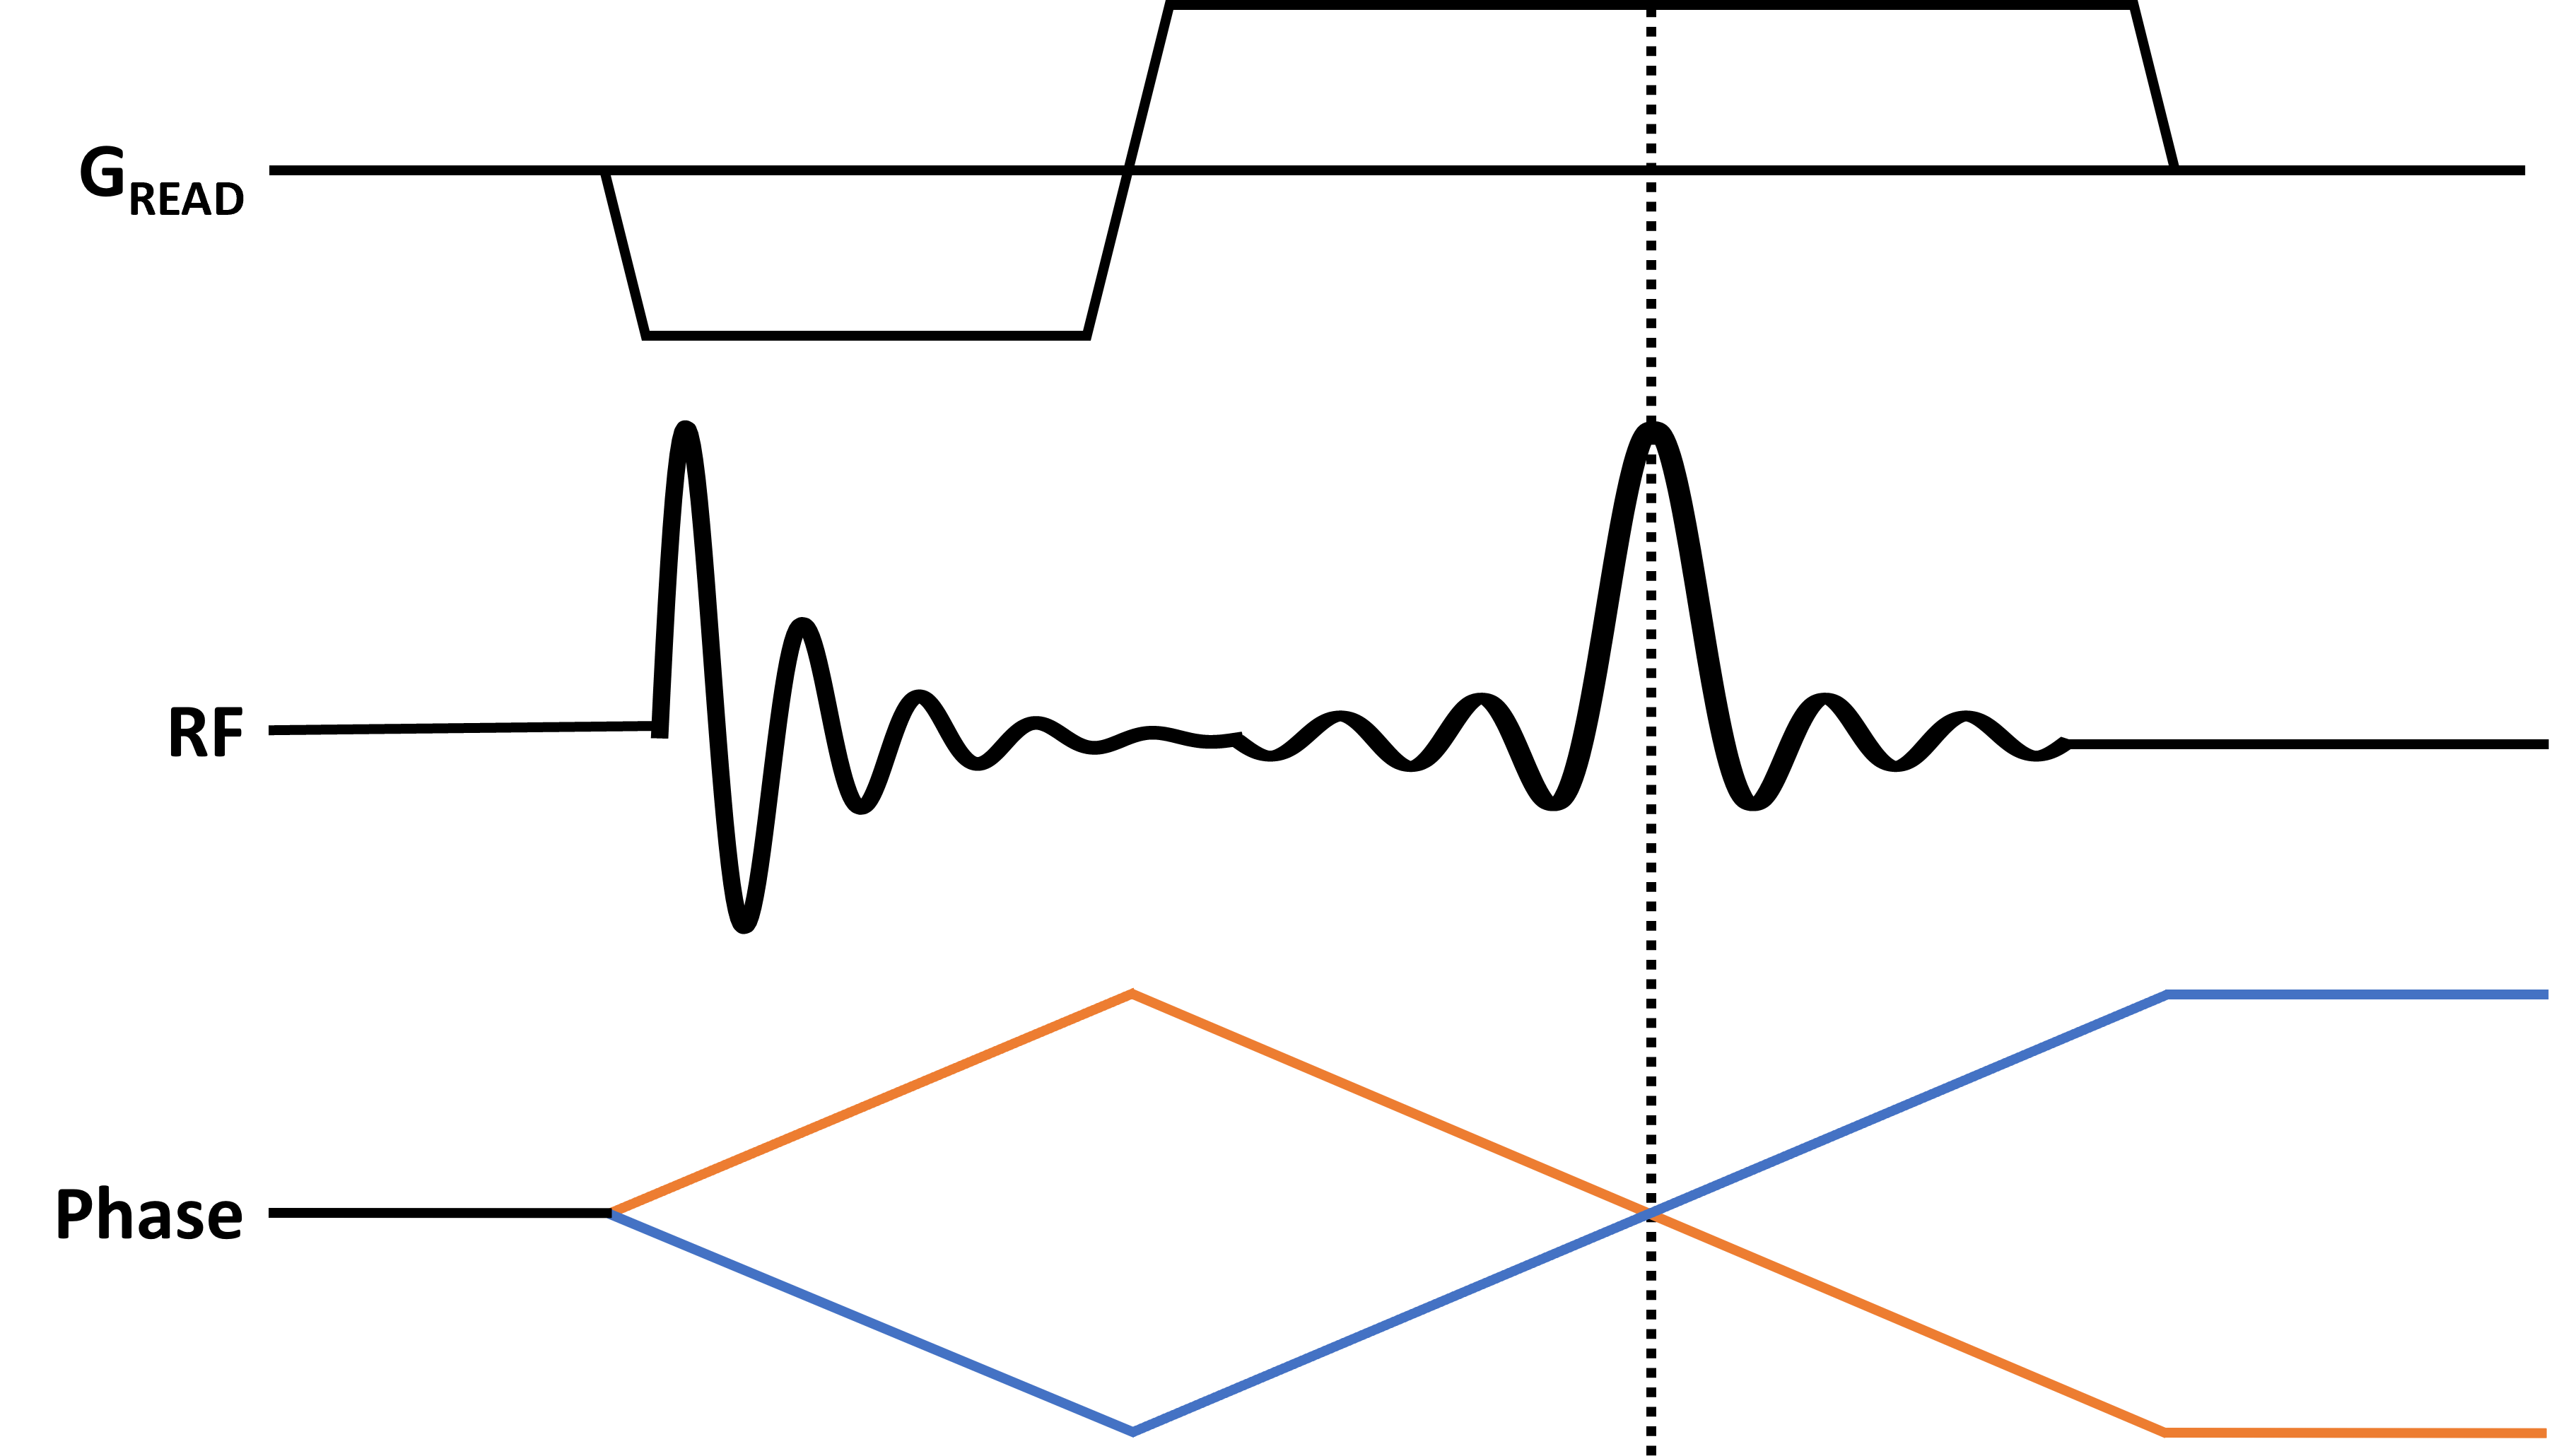
\includegraphics[width=0.9\textwidth]{Figures/Theory/RePhasing.png}
    \caption{Diagram showing how phase accumulation varies with dephasing lobes of the read gradient, along with the received \ac{RF} signal.}
    \label{fig:enter-label}
\end{figure}

The final spatial dimension is encoded using a phase-encoding gradient (G$_{phase}$) which is applied before the signal is acquired under the read gradient. This gradient only affects the phase of the signal in a way which is dependent on the position in real-space. By changing linearly changing the magnitude of the applied phase encoding gradient a set of 1D spectra are acquired which can be represented in a 2D matrix. The data in the 2D matrix is therefore a collection of spatial frequencies that are centred on 0, a low spatial frequency describes the general trend of an image whilst the high spatial frequencies define the sharp edges. This frequency space where the data is stored is called k-space, and applying a 2D \ac{FT} to this data produces an image \cite{Lauterbur1973ImageResonance, Mansfield1977Multi-planarEchoes}. The collection of \ac{RF} pulses and gradients is called a pulse sequence, and the pulse sequence described is called gradient-echo imaging, and can be viewed in Fig. \ref{fig:theory:GRE}.

\begin{figure}
    \centering
    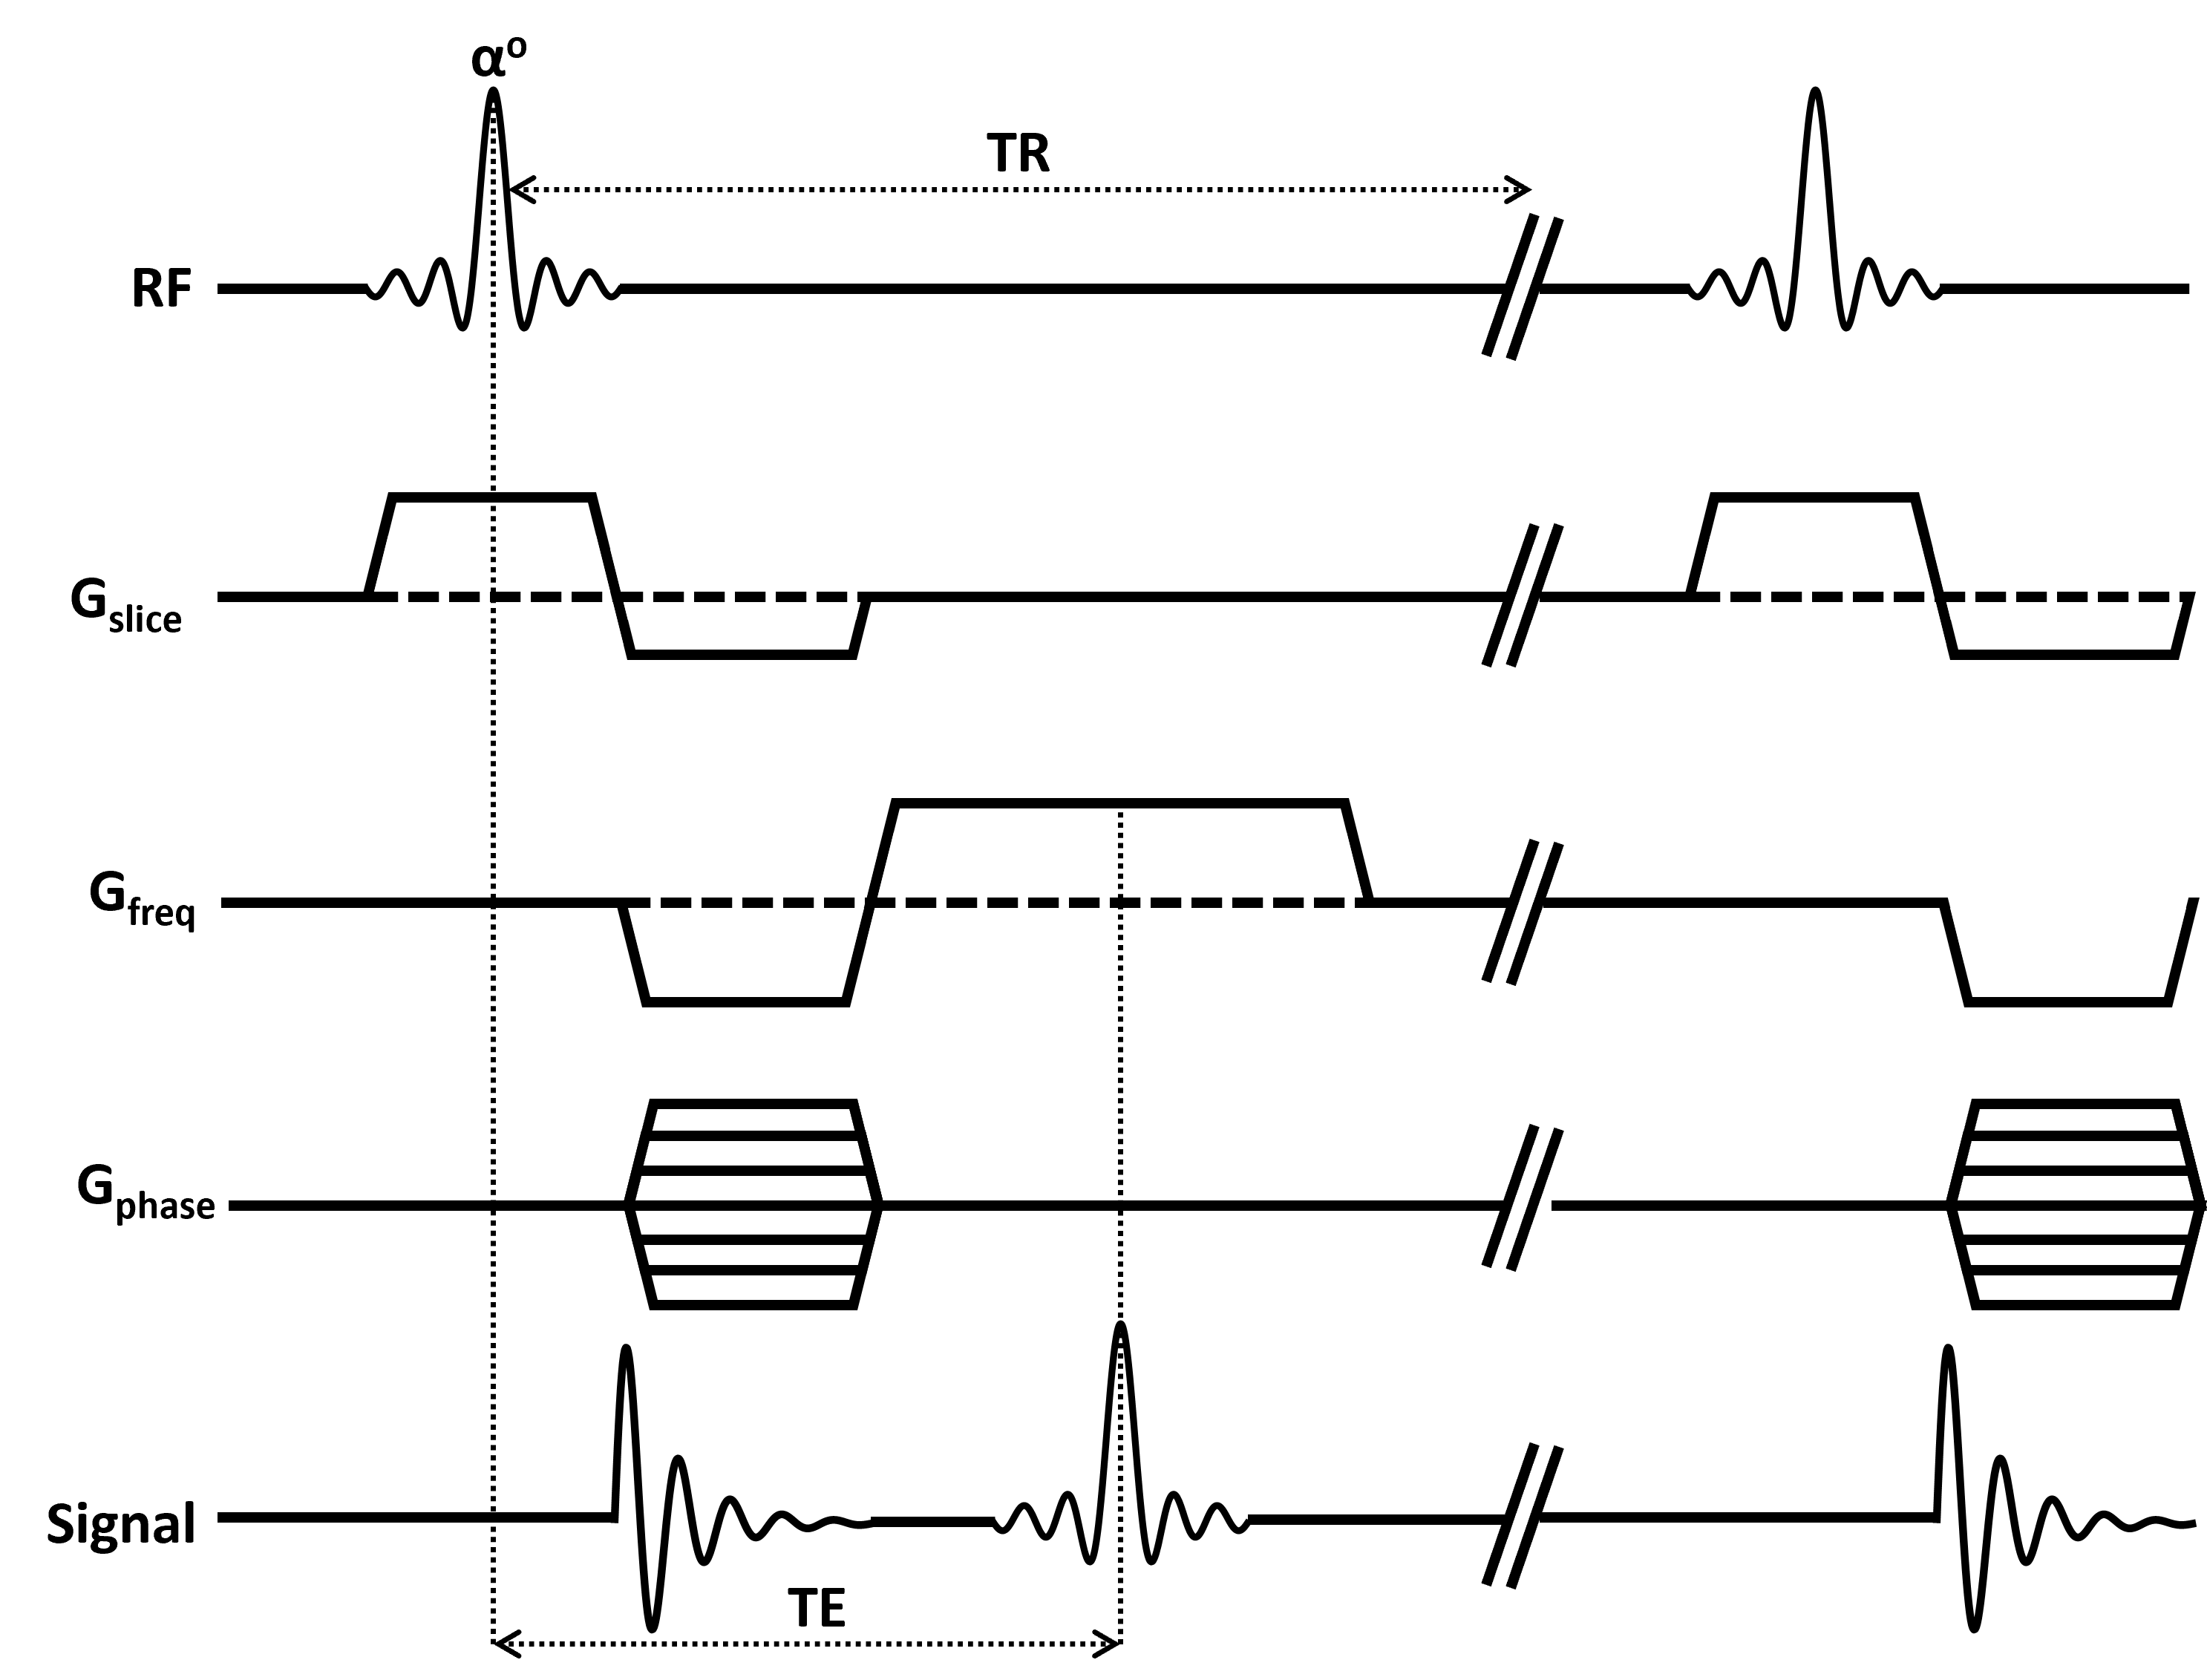
\includegraphics[width=0.8\textwidth]{Figures/Theory/GRE_sequence.png}
    \caption{\textit{Example pulse sequence diagram for a \ac{GE} imaging sequence, with the \ac{TE} indicated.}}
    \label{fig:theory:GRE}
\end{figure}

Longitudinal and transverse relaxation time constants vary depending on the type of tissue. Therefore, when a particular pulse sequence is used the choice of \ac{TR} and \ac{TE} will effect the the contrast in the image. The image signal varies with \ac{TR} and \ac{TE} according to Eq. \ref{eqn:theory:Signal}, which drives the contrast.

\begin{equation}
    S = M_0\sin(\alpha)\exp(-\textrm{TE}/T_2^*)\frac{(1-\exp(\textrm{TR}/T_1)}{(1-\cos(\alpha)\exp(-\textrm{TR}/T_1))}
    \label{eqn:theory:Signal}
\end{equation}

\noindent There are three main types of contrast in an image: T$_1$-weighted, T$_2$-weighted and spin density weighted. The contrast in spin-density images comes from the difference in the density of spins in a particular tissue being emphasised, remembering most commonly the spin of interest is $^1$H therefore its the proton density that gives the contrast. As expected then the contrast in T$_2$-weighted images is emphasised by differences in T$_2$ times of different tissues, in order to produce these images long \ac{TR}'s and long \ac{TE}'s are used which minimises effects from different T$_1$'s. Finally in T$_1$ weighted images the contrast is dominated by differences in the T$_1$ times of different tissues, this contrast is produced by choosing short \ac{TR}'s and \ac{TE}'s which minimise effects from different T$_2$ times. 

The \ac{SNR} obtained from a specific pulse sequence often depends on how quickly data can be acquired. One of the biggest aspects of scanning that affects the time taken is how data in k-space is obtained (k-space traversal). Therefore by traversing k-space more efficiently, scan time can be reduced which can make scanning more comfortable or can be used to improve \ac{SNR} by increasing averages. One of the biggest improvements in the traversing of k-space came with the development of \ac{EPI} \cite{Stehling1991Echo-planarSecond}.

\subsection{MRSI}

Acquiring MR spectra allows chemical and molecular concentrations to be obtained by comparing the magnitudes of peaks/signals at different chemical shifts. Whilst MR images provide good contrast for structural differences. It is possible to acquire information on both chemical/molecular concentrations as well as structural information using a technique called \ac{MRSI}, which is effectively a combination of \ac{MRS} and MRI. This technique works by acquiring spectra from small volumes that are packed together into a 2D/3D grid that covers a larger volume/tissue. The voxels are often much larger than what would usually be acquired using \ac{MRI}, but are much smaller than what would be acquired using \ac{MRS} strategies. By calculating concentrations for the visible molecules in each spectra the spatial distribution of each molecule can therefore be represented as a coarse image, this is often overlayed onto an anatomical images so that the corresponding regions can be easily identifiable. Concentration changes in specific tissues can therefore be used as bio-markers for disease. In order to obtain this type of data different pulse sequences are used that use different combinations of \ac{RF} pulses and gradients. 

\subsubsection{Chemical Shift Imaging}

\begin{figure}[h]
    \centering
    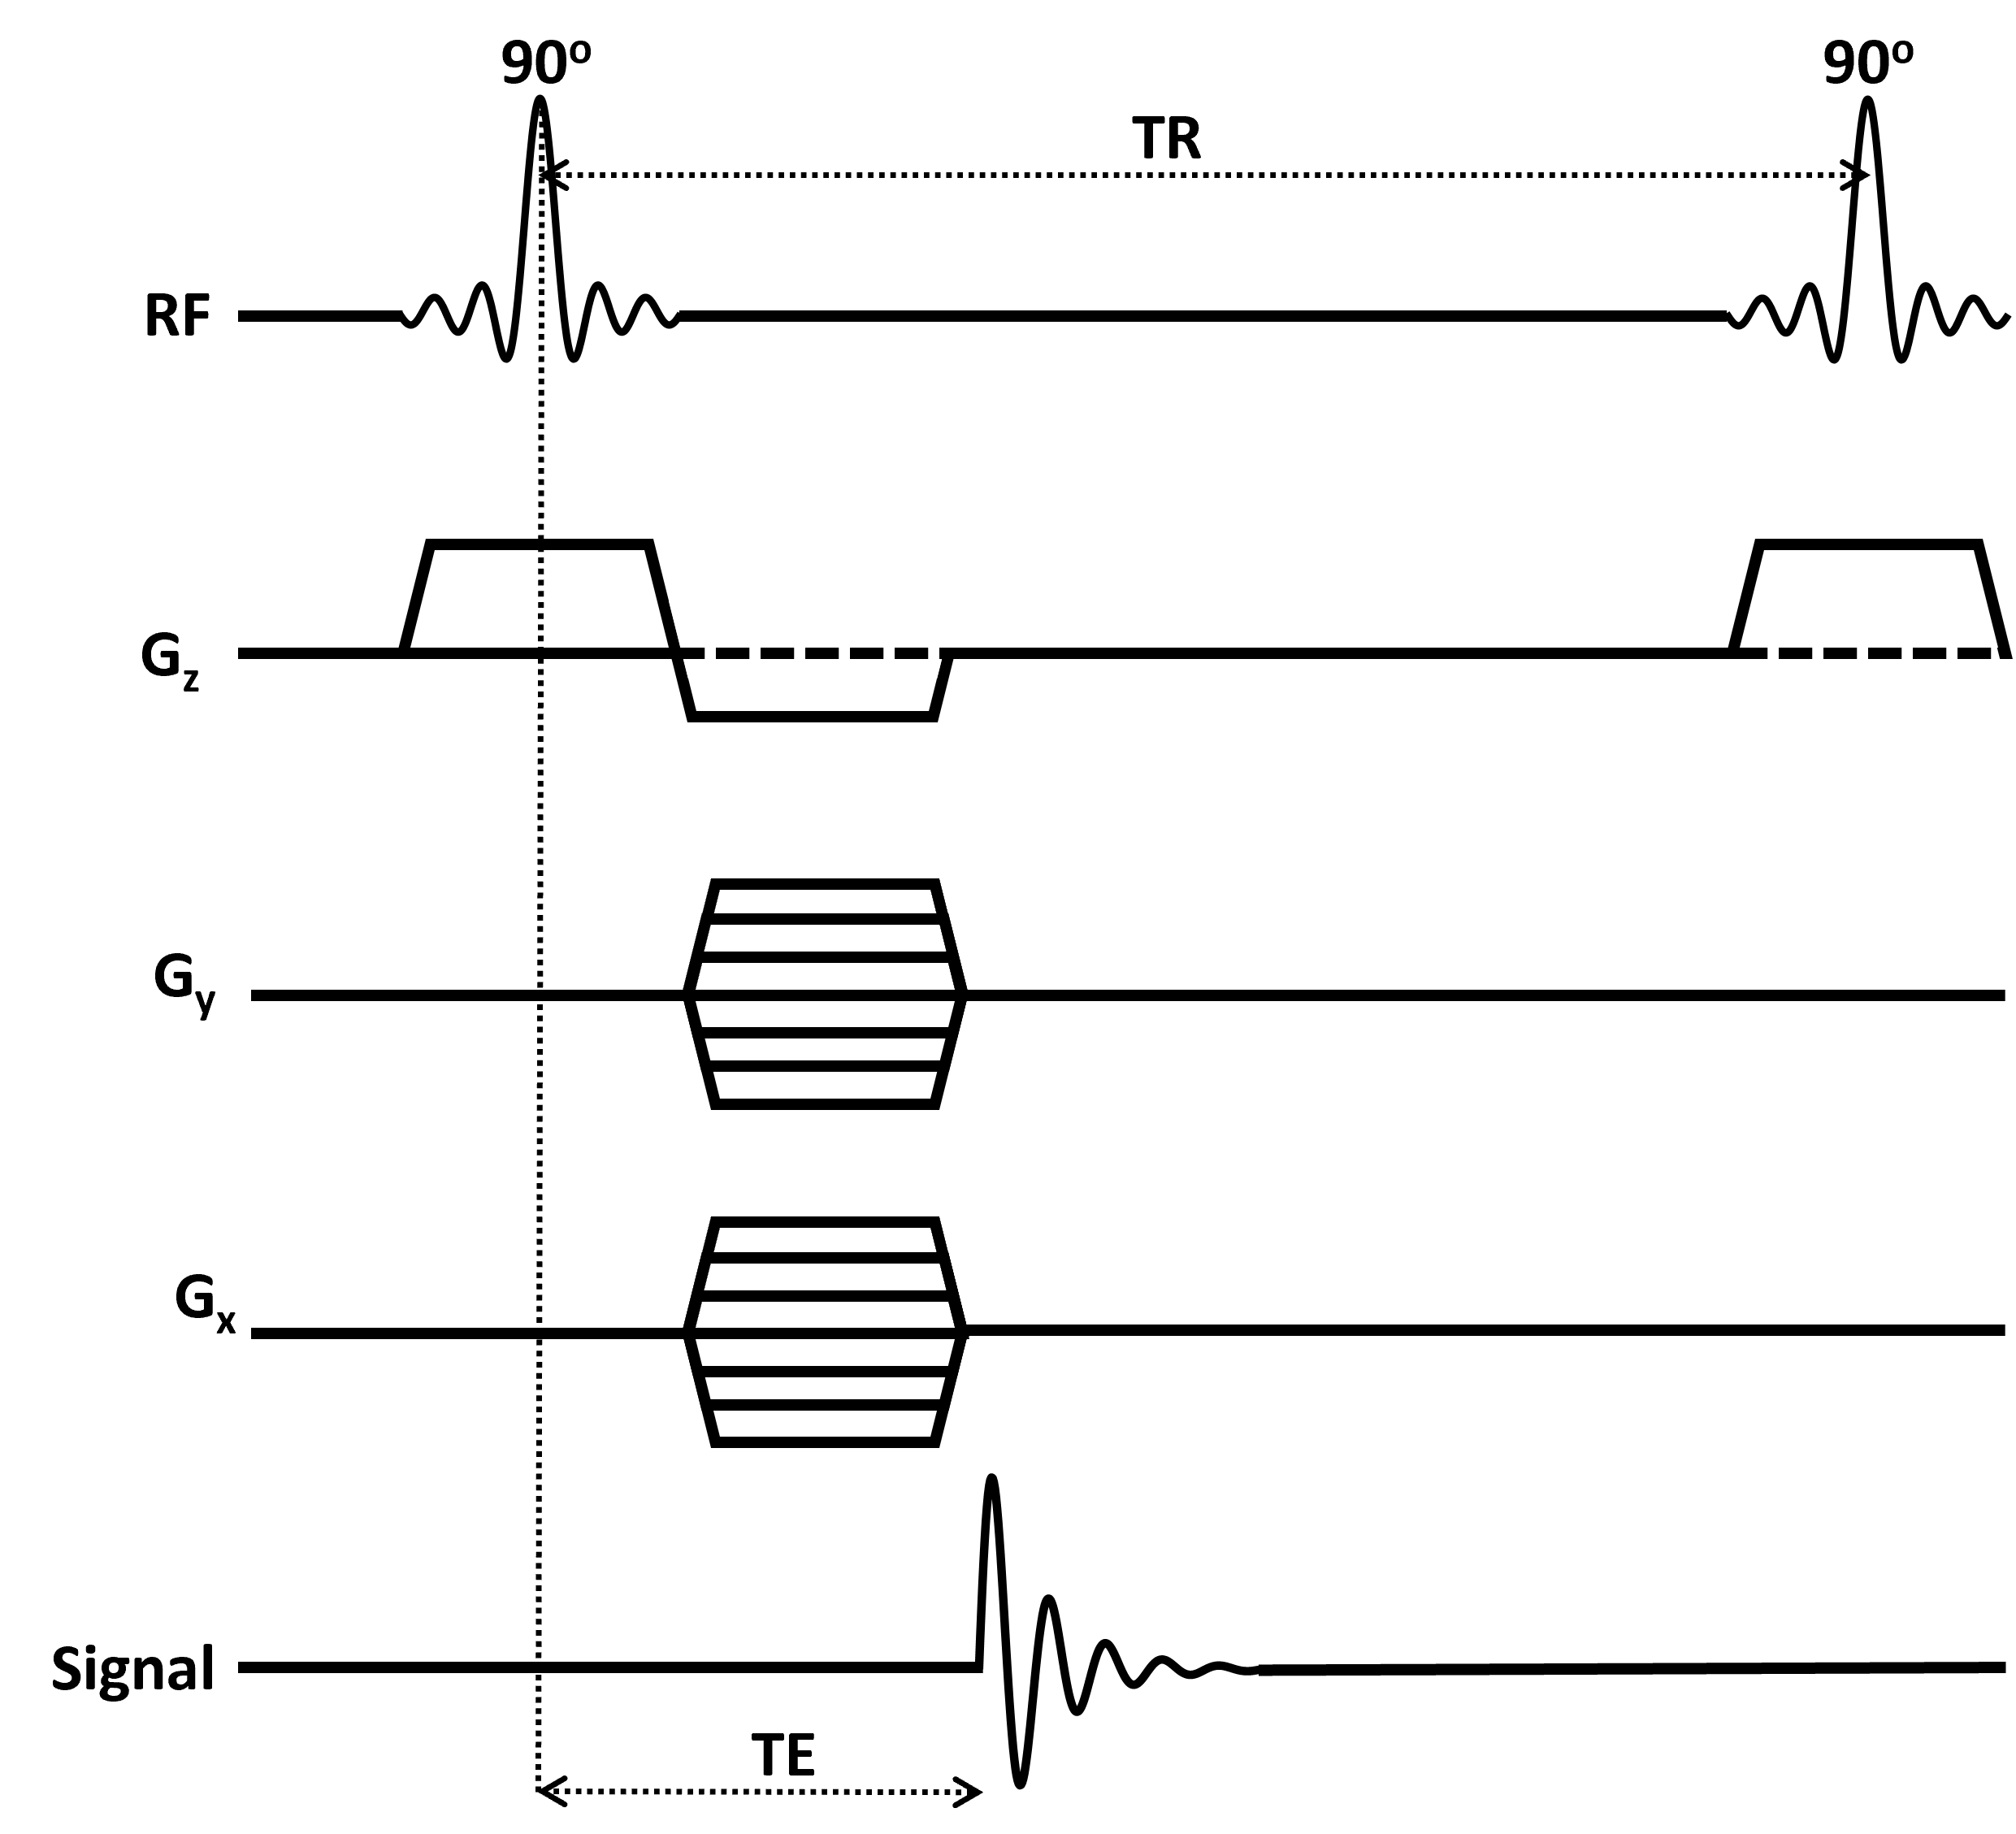
\includegraphics[width=0.9\textwidth]{Figures/Theory/CSI_sequence.png}
    \caption{\textit{Example pulse sequence diagram for a 2D \ac{CSI}.}}
    \label{fig:theory:CSI}
\end{figure}

The simplest and quickest method to acquire a spectrum is to apply an \ac{RF} pulse in a static magnetic field and acquire data from the FID immediately after the pulse. Application of a gradient during the \ac{RF} excitation will localise the data from a specific slice in the body. Usually this gradient is applied in the z-direction to localise the signal from a transverse slice through the body. However any direction of gradient can be used to excite a region. For example a sagittal or a coronal slice can be excited instead. The combination of these gradients increases the number of dimensions where data can be acquired, as has been shown with gradient echo imaging in Fig. \ref{fig:theory:GRE}. Therefore, by applying gradients in all three Cartesian directions simultaneously only data from a small voxel is excited, if data is acquired during the full length of an \ac{FID}that will only come from one small voxel. By iteratively changing the strengths of the adjacent voxels are excited eventually a full 2D/3D grid of spectra is obtained, this pulse sequence is called \ac{CSI}. A diagram of the pulse sequence used to acquire a 2D \ac{CSI} is shown in Fig. \ref{fig:theory:CSI}.

\ac{CSI} has been used for different nuclei ($^{13}$C, $^{31}$P and $^2$H) to create maps that show the distribution of different metabolites. Acquiring this type of data takes a long time which can be a problem is functional data was to be acquired, which motivates work to decrease the acquisition time for \ac{MRSI} data.

% \subsubsection{EPSI and SSFP}

% One of the first approaches developed for decreasing the imaging time was the introduction of \ac{EPI}. In usual \ac{GE} imaging the position in k-space returns back to zero, \ac{EPI} takes advantage of the position in k-space after an echo instead of letting it return to zero. By using multiple echoes and the use of small gradients to slightly change the position in k-space an entire 2D image can be obtained. Therefore \ac{EPI} refers to the use of a single \ac{RF} excitation to obtain an entire 2D k-space data-set. This has been implemented in imaging since 1977 \cite{Mansfield1977Multi-planarEchoes}. \ac{EPI} can also be applied to \ac{MRSI} to reduce scan times. This comes in the form of a relatively new pulse sequence called \ac{EPSI} \cite{Mulkern2001EchoImaging}. Unfortunately in \ac{MRI} there are very few situations where a positive benefit comes without associated negatives. This is no different with \ac{EPSI} as there is a reduction in \ac{SNR} that is equivalent to the reduction in scan time. The most common way to recover this \ac{SNR} is to increase the number of averages of the scan, however in order to recover all of the \ac{SNR} the averages needed would make a typical \ac{EPSI} and \ac{CSI} scan take the same amount of time \cite{Mulkern2001EchoImaging}. This may at first seem like a wasted exercise, however in some fields the reduction in \ac{SNR} maybe worth the trade-off as it makes \ac{MRSI} much more clinically viable. Also, since the \ac{EPSI} sequence has much more components than \ac{CSI} such as the gradients and echoes, there is more opportunity for development which can then improve \ac{SNR}, spectral resolution and/or scanning time even further. It has been shown that the use of multiple echoes can increase the spatial resolution without adding extra scan time \cite{Furuyama2011Multi-echo-basedScanner}. This has also been shown (along with an increased temporal resolution) by using acquisition in a single excitation and using parallel imaging (also called \ac{SENSE}) \cite{Posse2009Single-shotImaging}. Because of this and the useful trade-off between scan time and SNR, \ac{EPSI} has been successfully implemented in \ac{HP} metabolic imaging \cite{Topping2020AcquisitionNuclei,Eldirdiri2018DevelopmentScanner} and using $^2$H in the liver \cite{Min2023Deuterium7T}.

% \begin{figure}
    % \centering
    % 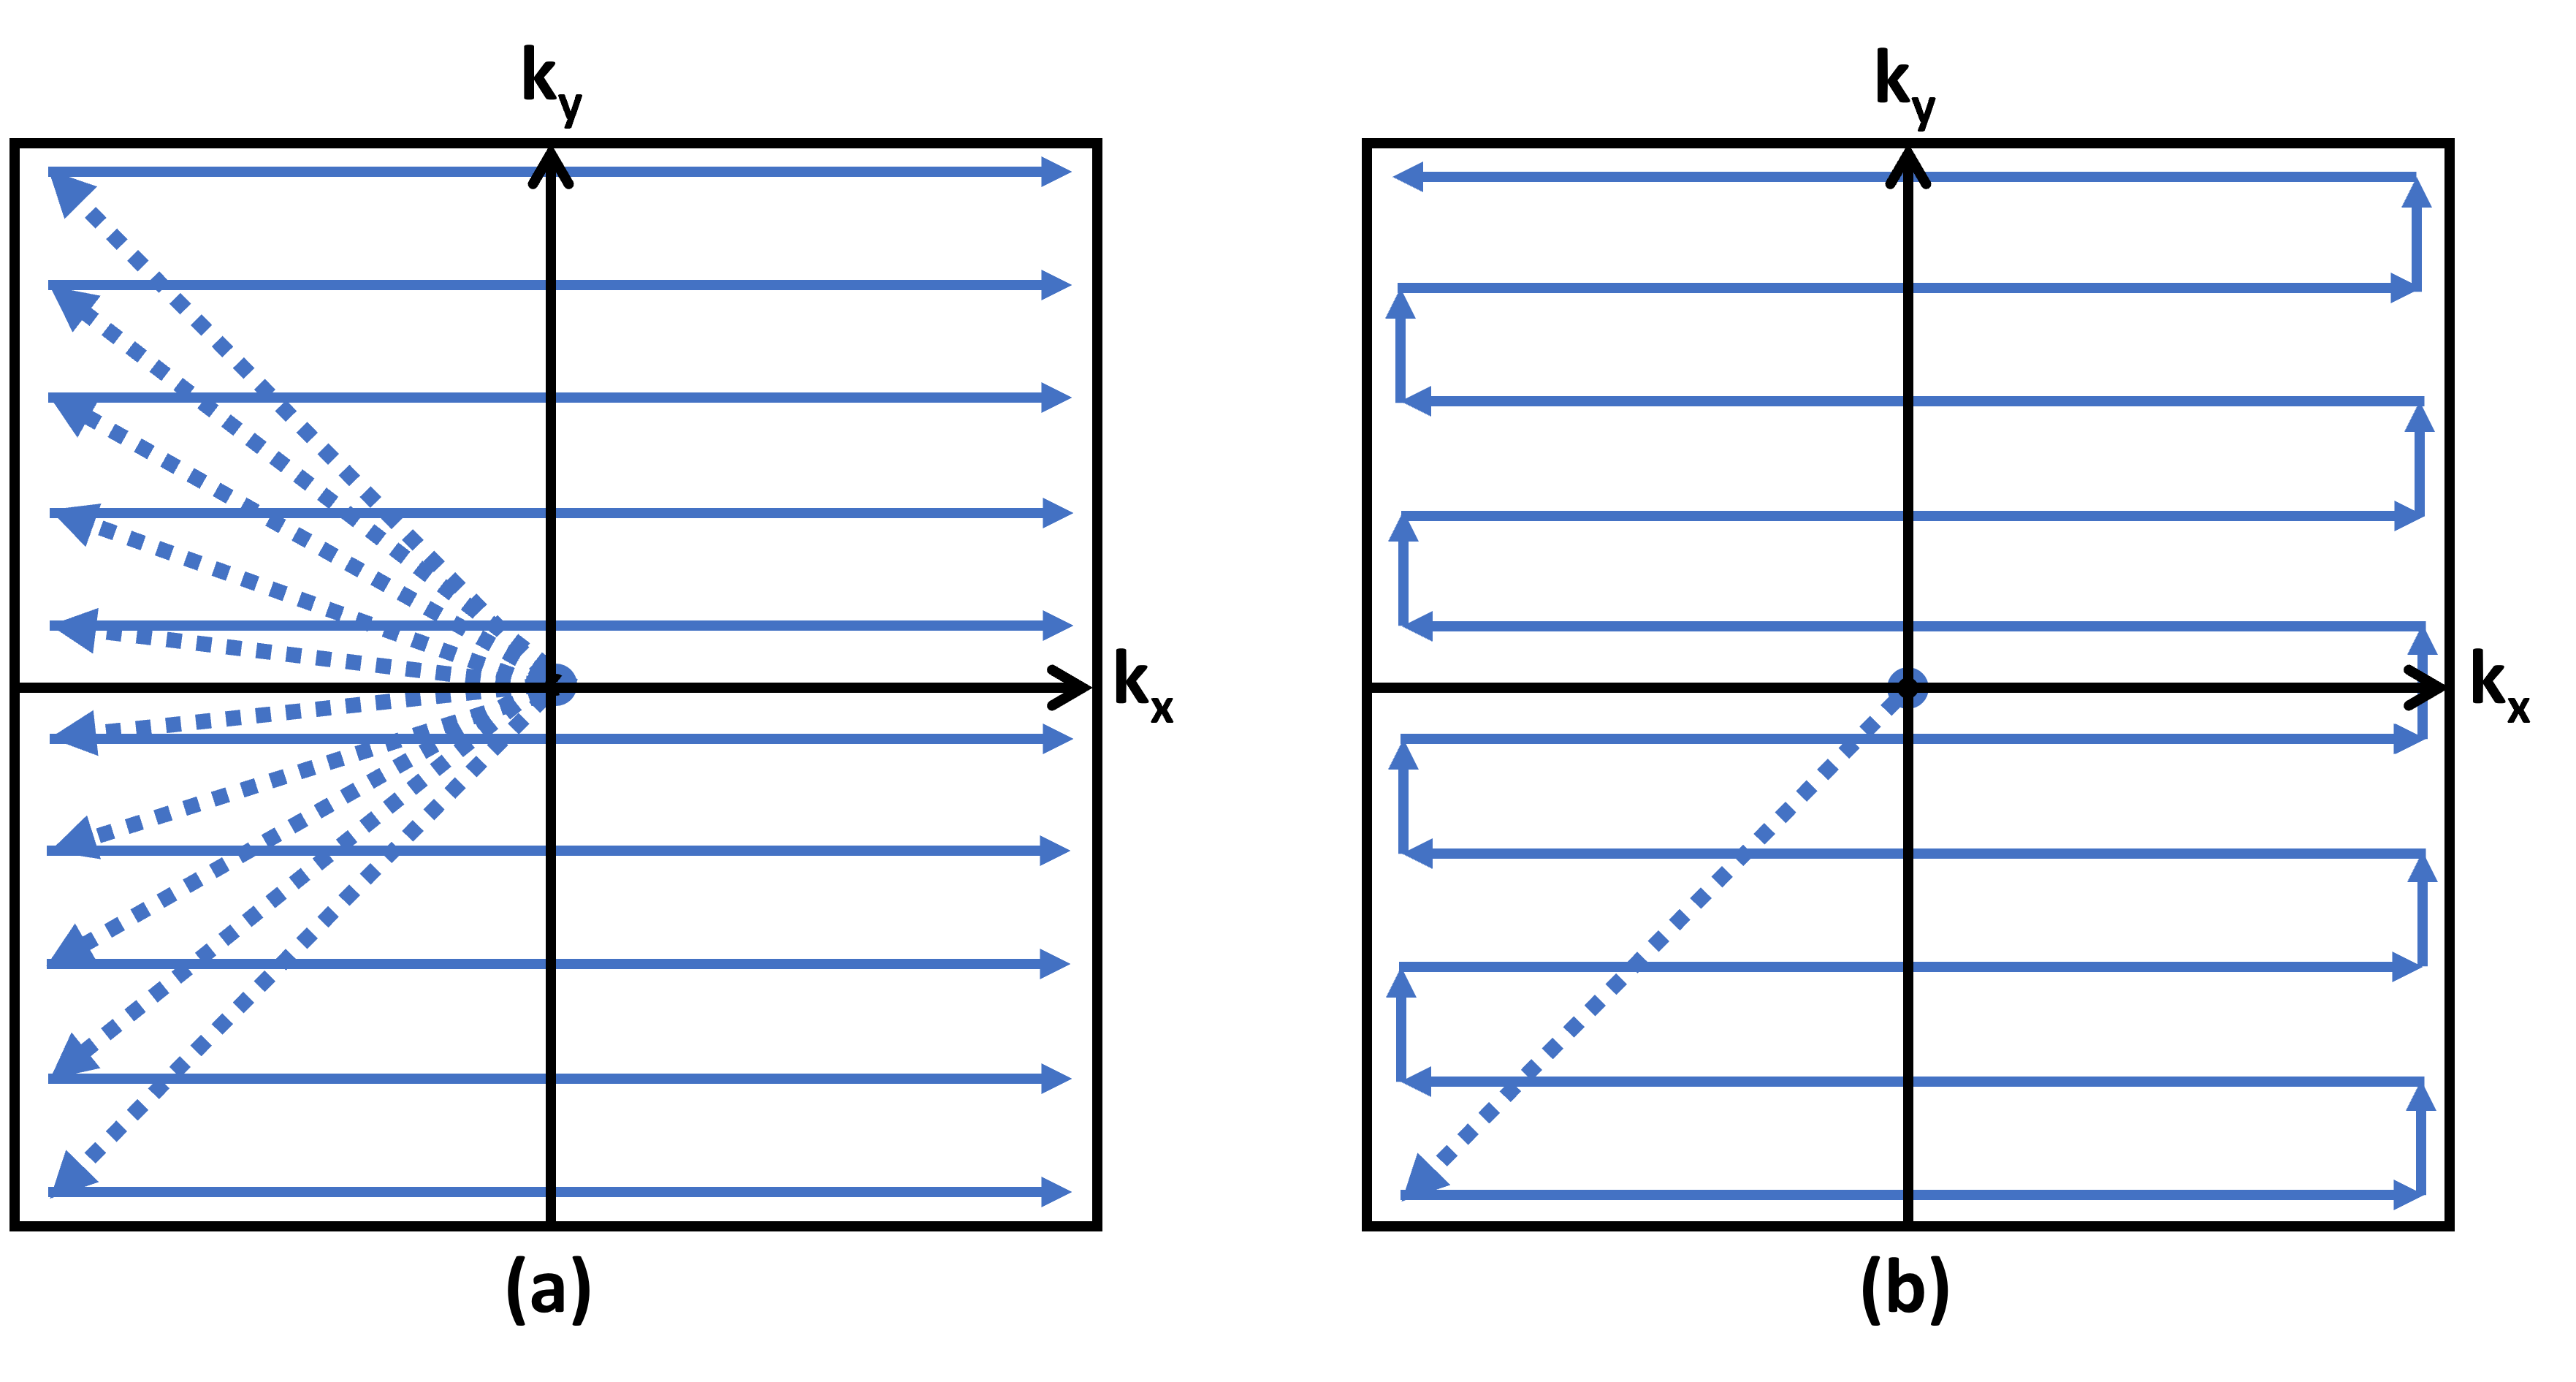
\includegraphics[width=0.9\textwidth]{Figures/Theory/kspace.png}
    % \caption{\textit{2D k-space traversal paths for a gradient-echo acquisition (a) and a echo-planar image acquisition.}}
    % \label{fig:theory:kspace}
% \end{figure}

% Balanced \ac{SSFP} \cite{Carr1954EffectsExperiments} is a special form of \ac{SSFP} where additional gradients are used to reduce off-resonance effects. \ac{SSFP} already known to increase \ac{SNR} compared to \ac{GE} imaging  \cite{Bieri2013FundamentalsMRI}, for situations where the T$_1$ to T$_2$ ratio is high (as \ac{SSFP} images have T$_1$/T$_2$ contrast). By using \ac{ME} \ac{SSFP}, with varying echo-times, it is possible to achieve good spectral separation of signals from the different metabolites, as the phase evolution between the metabolites across echoes will be different. So by combining the images for each echo as a non-linear problem using the IDEAL framework \cite{Reeder2007Water-fatImaging} metabolite maps, that appear similar to those acquired using \ac{CSI}, can be acquired. In doing this the \ac{SNR} enhancement of \ac{SSFP} is still maintained \cite{Peters2021ImprovingInvestigation}. The problem in doing this is the \ac{SNR} of this method will be higher for larger field strengths as the long echo-train needed to achieve phase separation of the different metabolite signals means that \ac{TR} is now too long to achieve sufficient \ac{SNR} gain (\ac{TR} $<<$ T$_1$ and T$_2$), this means the possible \ac{SNR} gain at lower field strengths needs to be explored. This has also only been performed for three different metabolites whereas this realistically needs to be able to analyse more metabolites which becomes much more complex. An alternative way of acquiring/analysing \ac{SSFP} data with spectrally separate metabolites is to alter the phase steps between successive \ac{RF} pulses in scans instead of the echo time, as it is much easier to separate multiple resonances and still keeps the \ac{SNR} increases of \ac{SSFP} which has been done using $^{13}$C \cite{Varma2016SelectiveSSFP}.

\section{Analysis}

\subsection{Quantification of MRS data}

When analysing \ac{MRS} data it is important to be able to accurately track changes for each spectra. The oldest method of doing this is peak integration whereby the spectral points are summed together. An integration range of at least two \ac{FWHM}'s is enough to get accurate quantification \cite{Near2021PreprocessingRecommendations}. The spectral peak integration value can also be obtained from the time-domain signal as the first point in the absorption spectra, as well as from the product of the \ac{FWHM}, $\pi$ and the spectral peak-height in the frequency domain \cite{deGraaf2019InSpectroscopy}. This technique is simple to implement computationally and takes little time, however it requires correctly phased spectra as any incorrect phasing will give the incorrect amplitude. Most biological tissues and processes involve complex chemical environments with many different compounds which will produce different MR signals appearing at different frequencies (also known as chemical shifts). This does not necessarily effect the peak integration method as long as each peak/signal has a large enough frequency offset relative to each other. However this is commonly not the case especially in $^1$H spectroscopy \cite{Alger2010QuantitativeReview}. 

Therefore, a different methodology is needed to overcome this issue, which comes in fitting spectral signal to lineshapes, such as Lorentzian \cite{Lorentz1895TheHeat}, Gaussian and Voigt \cite{Near2021PreprocessingRecommendations}. This is performed through a method called least-squares \cite{Golub1973TheSeparate} fitting whereby the sum ($R^2$) of the squared differences between the experimental data and a model (residuals) is minimised\cite{Vanhamme2001MRMethods}. Mathematically this is demonstrated in Eq. \ref{eqn:theory:LS}.

\begin{equation}
    R^2 = \sum_{i=1}^{n}[y_i - f(x_i,a_1,a_2,...,a_n)]
    \label{eqn:theory:LS}
\end{equation}

\noindent Where $i$ represents each data point with $n$ data points, and the range of values $a_1$ to $a_n$ covers the amount of fitting parameters such as linewidth (similar to \ac{FWHM}), frequency position, phase and most importantly amplitude. $R^2$ is said to be minimised when the following differential relationship for each fitting parameter is met, in Eq. \ref{eqn:theory:Diff} the derivative is referred to as the jacobian.

\begin{equation}
    \frac{\partial (R^2)}{\partial a_i} = 0
    \label{eqn:theory:Diff}
\end{equation}

\noindent The fitting begins by using initial parameter guesses and finds the sum of squared residuals. An optimisation algorithm is then used to update the parameter values iteratively, until a certain threshold in the $R^2$ value is met or the max number of iterations is used. The best way to model experimental \ac{MRS} data is in the time domain as a series of exponentially damped sinusoids. 

Since the full spectra comprising the sum many individual damped sinusoids is fit to the MR spectra. Therefore, the more signals present in the spectra the more difficult computationally this becomes. There is consequently a strong motivation to reduce the number of parameters, reduce the computational load and therefore increase the reliability of the fitting \cite{Near2021PreprocessingRecommendations}. It has been shown that one way to improve the reliability of fitting spectra that suffer from overlapping signals, which is the case for $^{31}$P \ac{MRS} data, is to use prior knowledge \cite{Hamilton2003PriorSpectra}. Some of the overlapping signals while distinctly different can share common ratios between some of their fitted parameter. One of the first fitting algorithms to include prior knowledge was the \ac{VARPRO} method \cite{Golub1973TheSeparate} which has successfully been used to analyse $^{31}$P data \cite{vanderVeen1988AccurateKnowledge,Stubbs199631P-MagneticADP}. Whilst \ac{VARPRO} was successful as an improved fitting methodology a new technique was recently developed called \ac{AMARES} which fits more reliably and accurately as well as having increased functionality, including lineshape choice, fitting echo signals and imposing upper and lower bounds on fitting parameters \cite{Vanhamme1997ImprovedKnowledge}. \ac{AMARES} is used regularly in \ac{MRS} analysis and is included in software packages such as JMRUI \cite{Stefan2009QuantitationPackage} and OXSA \cite{Purvis2017OXSA:MATLAB}, which have previously been used to analyse $^2$H \ac{MRS} data \cite{Simoes2022GlucoseGlioblastoma,Kreis2020MeasuringMRI,Kaggie2022DeuteriumMetabolism}. The model of summed damped sinusoids that is used in the \ac{AMARES} package is mathematically shown in Eq. \ref{eqn:theory:model}, with the trust region-reflective optimisation algorithm.

\begin{equation}
    y_n = \hat{y_n} + e_n = \sum_{k=1}^{k}a_k\exp(i\phi_k)\exp(-d_k(1-g_k+g_kt_n)t_n)\exp(i2\pi f_kt_n) + e_n
    \label{eqn:theory:model}
\end{equation}

\noindent $k$ is the number of sinusoids, $\phi_k$ is the phase, $d_k$ is the damping factor, $g_k$ determines the lineshape (1 for Gaussian, 0 for Lorentzian), $t_n$ is the time for each point, $f_k$ is the frequency offset and $e_n$ is comples white Gaussian noise. The caret represnts the model as oppose to actual measurments.

Even \ac{AMARES} has its limits and signal fitting can struggle when many peaks are present especially in terms of overlapping signals, which is a big problem in $^1$H \ac{MRS} data. Therefore, a new methodology was developed to overcome this called linear combination and was made into a toolbox that is still used called LCModel \cite{Provencher1993EstimationSpectra}. This works by fitting total spectra for each metabolite (called basis sets) instead of individual peaks, this reduces the number of model parameters and leads to increased reliability in fitting. The basis sets can be acquired by either phantom \textit{in vitro} experiments or by numerical simulation \cite{Near2021PreprocessingRecommendations}. Because of this it is more complicated to set up so it is yet to be used commonly for the more simplified and sparse spectra from $^{13}$C, $^{31}$P and $^2$H, although it has been used in analysing data for the indirect detection of $^2$H glucose by looking at the loss in $^1$H signal \cite{Rich20201HVivo,Cember2022IntegratingHumans,Niess2023Reproducibility3T}. 

\subsection{Post-Processing Improvement of SNR}

The low \ac{SNR} of $^2$H is often a problem during scanning and as scanning times are reduced for participant/patient comfort this can be a problem in spectroscopy with any nuclei. Whilst fitting in the frequency domain can provide accurate fitting and quantification, it is now common practise to fit data in the time-domain which can have the ability to provide more accurate and reliable fitting \cite{Joliot1991InMethods}. In order to increase the reliability and reproducibility of values obtained from analysis it is important to maximise the \ac{SNR}. A popular method of increasing the \ac{SNR} of spectra is to apply spectral filtering in the form of apodisation. Common lineshapes that are used in the filtering are exponential and Gaussian \cite{Goryawala2020EffectsFitting}. Applying a Gaussian filter can reduce the \ac{FWHM} of MR signals which can improve fitting reliability however this will change the lineshape of the signal, the best way to do this is to apply an exponential filter along with a Gaussian to negate the previous lineshape such that the new signal is only Gaussian. However, it has been shown that apodisation can reduce accuracy of fitting especially in cases of complex spectra where signals overlap spectrally \cite{Bartha1999FactorsFiltering}. Because of this apodisation is often used sparingly and often only used for visual demonstrations of data. Lots of alternatives exist in terms of denoising including \ac{PCA} \cite{Abdoli2016DenoisingComponents} and low rank approximation \cite{Nguyen2013DenoisingApproximations} that have been shown to provide improved \ac{SNR} with limiting quantification \cite{Clarke2022UncertaintyMethods}. 

\ac{SVD} is a linear algebra technique that breaks down a 2D matrix into its key components, and is used to reduce a matrix without affecting the data. An example would be a 2D matrix $A$ that is $m$ x $n$ in size will have $m$ x $n$ values, if this can be decomposed into two vectors that are orthogonal such that $A$ = $\mathbf{uv}^\textrm{T}$ the total number of values in these vectors is $m+n$. Therefore large data sets can be sent easier with a smaller storage size without compromising on the data itself. The \ac{SVD} starts off originally as an eigenvalue problem with $\sigma$ representing the eigenvalue $u$ and $v$ are eigenvectors. The eigenvalue problem only works when $A$ is to be a square matrix, if $A$ is a rectangular matrix with $m$ x $n$ size the eigenvectors become square matrices with sizes $m$ x $m$, $U$ and $n$ x $n$ $V$. Where each column of $v$ and each row of $u$ diagonalizes the matrix $A$ similar to an eigenvalue problem.

\begin{equation}
    A \mathbf{v}_n = \sigma_r \mathbf{u}_m
\end{equation}

\noindent Where $r$ is the `rank' of the matrix and contains all the key components of $A$. The eigenvalues then form the diagonal elements of the matrix $\Sigma$ called the `core matrix', the eigenvalues are called the singular values and the size represents the importance for reconstructing $A$. By rearranging the matrices Eq. \ref{eqn:theory:SVD} is created for the matrix $A$.

\begin{equation}
    A = U\Sigma V^\textrm{T} = \sum_{k=1}^{r} u_k\sigma_kv_k^\textrm{T}
    \label{eqn:theory:SVD}
\end{equation}

\noindent However, a full reconstruction does not necessarily need to be performed, if the core matrix is arranged by size and the lower singular values are removed $A$ can be reconstructed with only the more important features. When this technique is applied to \ac{MRS} data this will de-noise the data as the noise will be represented by the lower singular values \cite{Brender2019DynamicHyperpolarization}. This technique can also be also used to fit \ac{MRS} data as the results can be converted into the regular fitting parameters \cite{Pijnappel1992SVD-basedSignals}, as well as to remove water signal post-processing \cite{Cabanes2001OptimizationBrain}.

This only works in 2D matrices, which is an issue for \ac{MRSI} data which commonly has up to five dimensions (one spectral, three spatial, and a temporal domain). A similar technique can be used in this case called \ac{HOSVD} which is similar to regular \ac{SVD} but has the ability to work with higher dimension data. Here the matrix is decomposed into a collection of tensors $U$ equal to the number of dimensions of $A$ which is $d$, along with a core tensor $S$. The mathematical form of this decomposition is shown in Eq. \ref{eqn:theory:HOSVD}.

\begin{equation}
    A = S \otimes U_1 \otimes U_2 \otimes ... \otimes U_d
    \label{eqn:theory:HOSVD}
\end{equation}

\noindent This gives a core tensor that is the same size in each dimension, this can be truncated in a similar way to \ac{SVD} so that when the original matrix $A$ is reconstructed the lower important components are removed. For \ac{MRSI} data this de-noises the data as the lower singular values again represent the noise. The core tensor here will have the same size in each dimension, which is not optimal for \ac{MRSI} data as often the spectral dimension will be much larger than the spatial or temporal dimensions. To overcome this a Tucker decomposition is used which allows a core tensor of any size to be constructed \cite{Tucker1966SomeAnalysis}, this gives much more control over the level of de-noising that is applied. This whole method is called a Tucker-Tensor decomposition and has been used previously to de-noise \ac{DMI} data \cite{Kreis2020MeasuringMRI, Assmann2020InCholesterol}. This strategy has been implemented in this work using a MATLAB toolbox \cite{Bader2007EfficientTensors}.

% \subsection{Concentration Calculation} % Potential
% Robins section from glucose paper 

\section{RF Coils}

\ac{RF} coils have two functions: to first apply a B$_1$ field to excite spins into specific energy levels or orientation's, and second to receive a signal from precessing magnetisation Faraday's law of induction. The profile of the applied B$_1$ field is due to the design/shape of the coil, the sensitivity of the coil also depends on the electronic components used for tuning and matching. The frequency of the applied $B_1$ depends on the applied waveform. The key point in designing/building the \ac{RF} coil is to maximise the $B_1$ per unit voltage by tuning the coil to resonate at the Larmor frequency and matching the coil's impedance to whatever it is connected to. This shows how important design and building of \ac{RF} coils is. Lots of different companies exist from whom it is possible to buy \ac{RF} coils. This can be expensive due to the experience and time that goes into coil building. Therefore it is useful when starting new research with a new nuclei (such as $^2$H) to be able to build home-made coils. 

\subsection{Theory}

% the voltage and current and the relationship with phase can be demonstrated through a phasor diagram which can also represent complex numbers. Therefore, many electrical components can also be represented as complex numbers. The current variation with time ($I(t)$) of an RLC circuit is shown in Eq. \ref{eqn:theory:Current}.

% \begin{equation}
    % I(t) = I_{\mathrm{max}}\sin(\omega t + \phi)
    % \label{eqn:theory:Current}
% \end{equation}

% According to Ohm's law the voltage across a resistor ($\Delta V_R$) can be found, an inductor will oppose the current and will therefore have a corresponding reactance ($X_L$) and will be 90$^\circ$ ahead of the current. The time-varying voltage will cause the capacitor to continuously charge and discharge which resists the change in voltage and will also have a reactance ($X_C$). 

The simplest way to build an \ac{RF} coil is to shape a wire into a loop (inductor) and connect a capacitor in parallel. This forms what is known as an LCR circuit which is often used to create a resonance for current. The LCR circuit will have a natural resonance frequency ($\omega_0$), therefore when the frequency of the applied current is the same as this natural frequency the circuit is considered on resonance ($\omega=\omega_0$). For a circuit to resonate the opposition of the (alternating) current flowing through the circuit, referred to as reactance ($X$), needs to be minimised. $X$ is the imaginary component of the impedance given as $Z = R+iX$, and for an LCR circuit is composed of two components the inductive reactance ($X_L$) and the capacitive reactance ($X_C$). The total reactance for a series LCR is the difference between $X_L$ and $X_C$, for a parallel LCR circuit the reciprocal of the total reactance is equal to the sum of the reciprocal of the individual components. The relationship between the reactances and the resonant frequency is shown in Eq. \ref{eqn:theory:X}.

\begin{equation}
\begin{gathered}
    X_L = i\omega L \\
    X_C = \frac{1}{i\omega C}
    \label{eqn:theory:X}
\end{gathered}
\end{equation}

The resonant condition of the LCR circuit is then well demonstrated well calculating the current flow, which is shown in Eq. \ref{eqn:theory:I} as the ratio between the voltage and the impedance.

\begin{equation}
    I = \frac{V}{Z} = \frac{V}{R+i(\omega L - \frac{1}{\omega C})} = \left| \frac{V}{\sqrt{R^2+(\omega L - \frac{1}{\omega C})^2}} \right|
    \label{eqn:theory:I}
\end{equation}

The natural resonance of the circuit is therefore given in Eq. \ref{eqn:theory:res}.

\begin{equation}
    \omega_0 = \frac{1}{\sqrt{LC}}
    \label{eqn:theory:res}
\end{equation}

The voltage variations with time for each electrical component is shown below in Eq. \ref{eqn:theory:Voltage}. As an \ac{RF} $B_1$ is applied to the coil, current will be induced which charges the capacitor. As the $B_1$ is then removed, the capacitor will then dissipate energy which causes current to flow through the rest of the circuit. Energy dissipates and therefore current decreases exponentially. Graphs of the change in voltage in this case are shown in Fig. \ref{fig:theory:VI}, along with the corresponding absorption and dispersion curves. This behaviour is often referred to as an impulse response.

\begin{equation}
\begin{gathered}
    \Delta V_R = IR = I_{\mathrm{max}}R\sin(\omega t + \phi) \\
    \Delta V_L = \omega LI_{\mathrm{max}}\cos(\omega t + \phi) =  X_LI_{\mathrm{max}}\cos(\omega t + \phi)\\
    \Delta V_C = -\frac{I_{\mathrm{max}}}{\omega C}\cos(\omega t + \phi) = -X_C\cos(\omega t + \phi)\\
    \label{eqn:theory:Voltage}
\end{gathered}
\end{equation}

The most common cables that are used to connect to \ac{RF} coils are coaxial cables, which usually have a characteristic impedance of 50$\Omega$. When a coil is constructed and tuned to the Larmor frequency the impedance is most likely different to the impedance of the cable. The difference in impedance will cause some of the power to be reflected at the coil instead of transmitted. Therefore, the impedance of of the coil needs to be changed which can be done by changing its reactance. The most common ways of doing this are by adding an inductor or a capacitor in parallel to the coil. The method of adding a capacitor will be discussed here and an example circuit can be seen in Fig. \ref{fig:theory:RLC}.

\begin{figure}
    \centering
    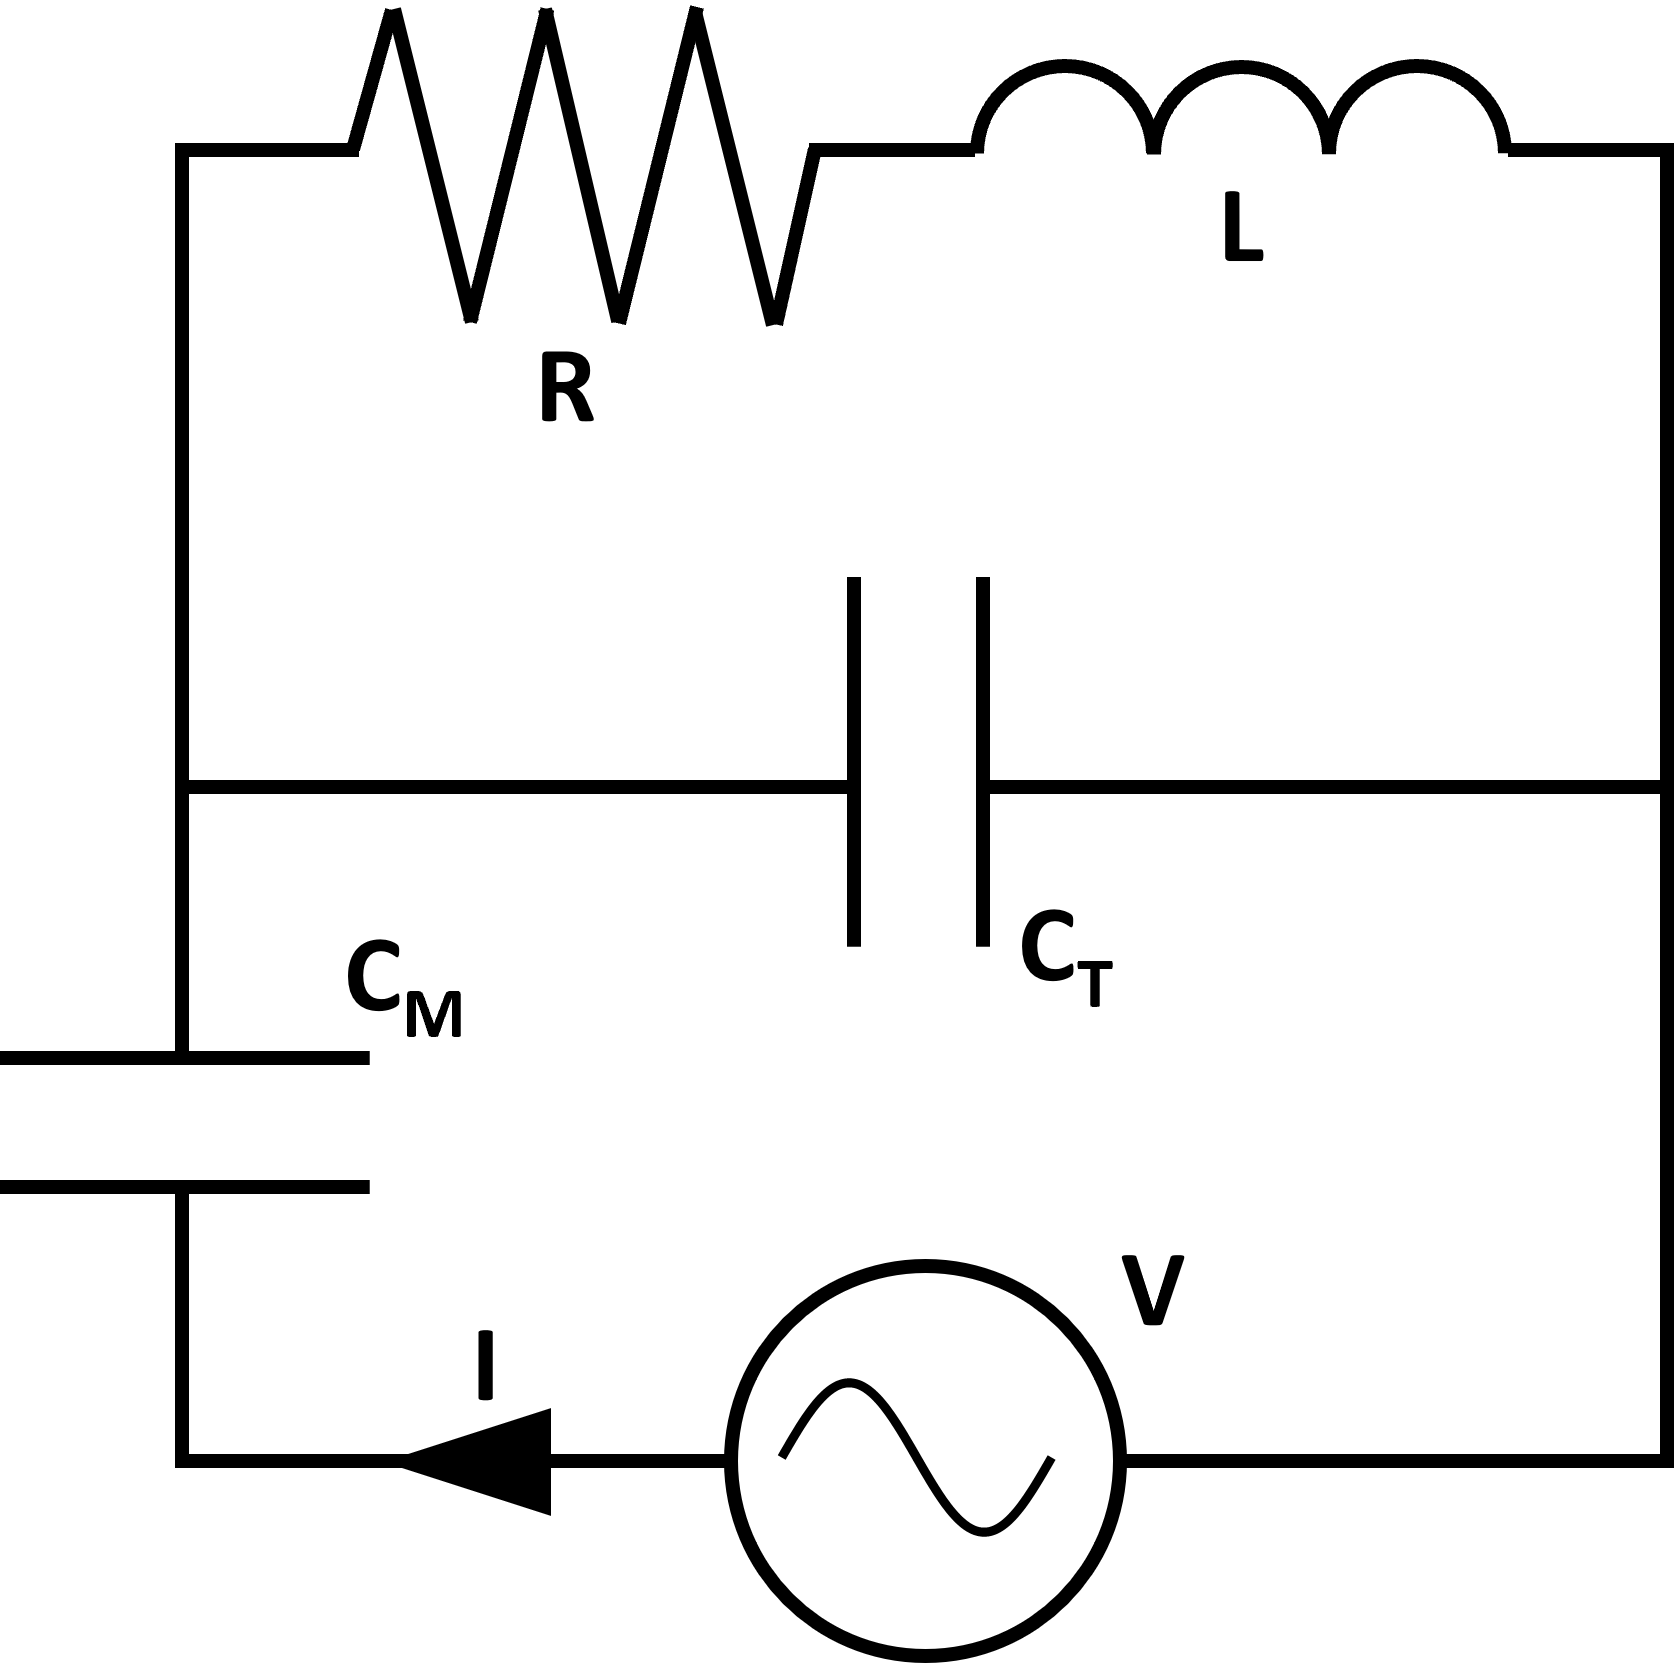
\includegraphics[width=0.6\textwidth]{Figures/Theory/RLC_Circuit.png}
    \caption{\textit{Example diagram of an LCR circuit with both tuning (C$_T$) and matching capacitors (C$_M$), along with an AC signal generator.}}
    \label{fig:theory:RLC}
\end{figure}

The capacitor in series with the coil is referred to as the tuning capacitor (C$_T$) with the other capacitor called the matching capacitor (C$_M$). The total capacitance is C$_M$+C$_T$. A relationship between C$_M$ and C$_T$ can be found that is related to the quality factor (Q) \cite{Chen1989ChapterNoise} which is the resonance frequency divided by the bandwidth of the coil resonance in Fig. \ref{fig:theory:VI}, and is shown in Eq. \ref{eqn:theory:match}. 

\begin{equation}
    C_M = \sqrt{\frac{C_T}{Q\omega_0Z}}
    \label{eqn:theory:match}
\end{equation}

The combination of Eqs. \ref{eqn:theory:res} and \ref{eqn:theory:match} can be used to find the capacitances needed to tune and match the coil \cite{Chen1989ChapterNoise}. To test a fully constructed coil an \ac{AC} is applied to the coil and the reflected power is plotted against frequency as a logarithmic scale measured in decibels (dB), the graph will appear similar to the absorption spectra shown in Fig. \ref{fig:theory:VI}. A level of 20 dB is commonly perceived as a good enough value of reflected power, with the peak appearing at the Larmor frequency. Realistically soldering and adding components will change the circuit and the theoretical components can be wrong so will often need changing based on the measured response.

\begin{figure}
    \centering
    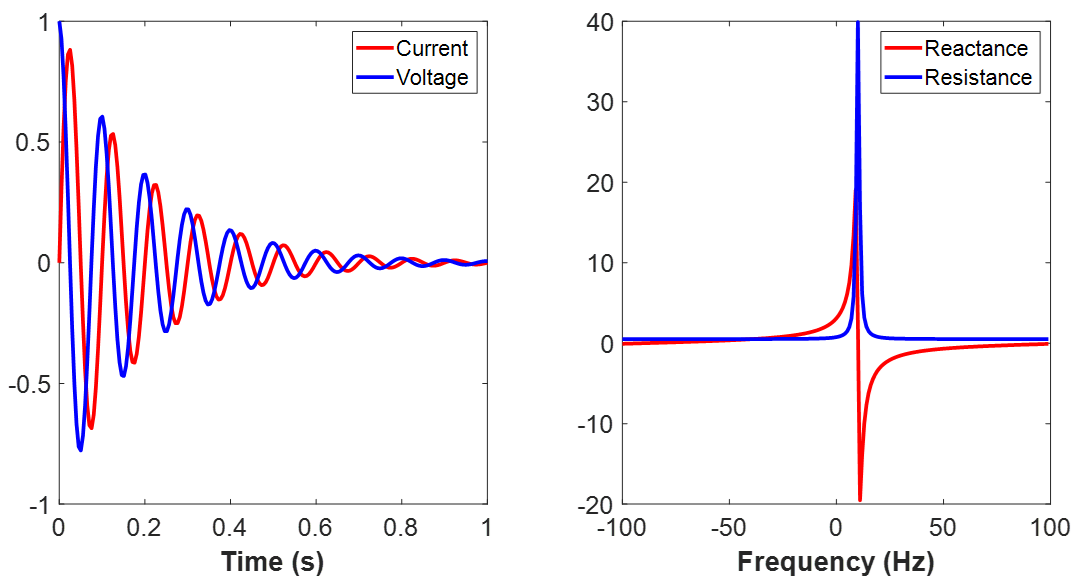
\includegraphics[width=0.9\textwidth]{Figures/Theory/VI.png}
    \caption{\textit{(a) Current and Voltage graphs for a dissipating capacitor in an RLC circuit. (b) corresponding absorption and dispersion spectra that show resistance and reactance respectively.}}
    \label{fig:theory:VI}
\end{figure}

When a coil is placed over a sample or body tissue coupling occurs which changes the total current impedance. This changes the matching condition as well as the resonant frequency of the coil. Therefore it is important to load the coil with a phantom that matches the loading response that will be present during scanning, when designing/building the coil. 

\subsection{Coils Built}

Three different coil types were constructed to use in the experiments reported here and implemented for use on a Philips 3T Achieva system. These were two surface coils, a saddle coil and a Helmholtz coil. All coils were tuned to 19.6 MHz, the Larmor frequency of $^2$H at 3T. A 2 L salt-water solution was used to load each coil, since each coil was used for scanning on different body parts the loading response changed slightly which was controlled by changing the salt concentration. A birdcage coil dual tuned to the Larmor frequencies of $^1$H and $^2$H at 7T was purchased from Rapid Biomedical for use on a 7T Philips Achieva System. The in-house built coils were used to acquire spectroscopic $^2$H data with anatomical $^1$H images being acquired using the whole-body \ac{RF} coil in the scanner for transmission and reception. The purchased coil is able to acquire $^1$H anatomical images as well as $^2$H spectroscopic data, low resolution $^2$H images were also acquired using this coil.

\subsubsection{Surface Coil}
\label{Chap:Theory:Coils}

A surface coil is the simplest and most basic coil to design, where the coil often forms a simple circular loop. The magnetic field is maximum directly in the centre of the coil and decreases, with distance from the coil. Therefore the field is spatially in-homogeneous which is why this coil design is often used for non-localised spectroscopy, where the localisation of the signal is down to the placement of the coil. The penetration depth of the magnetic field for a surface coil is approximately equal to the diameter of the coil \cite{Gruber2018RFNonphysicists}, and therefore is sensitive to regions closest to the coil. 

\begin{figure}
    \centering
    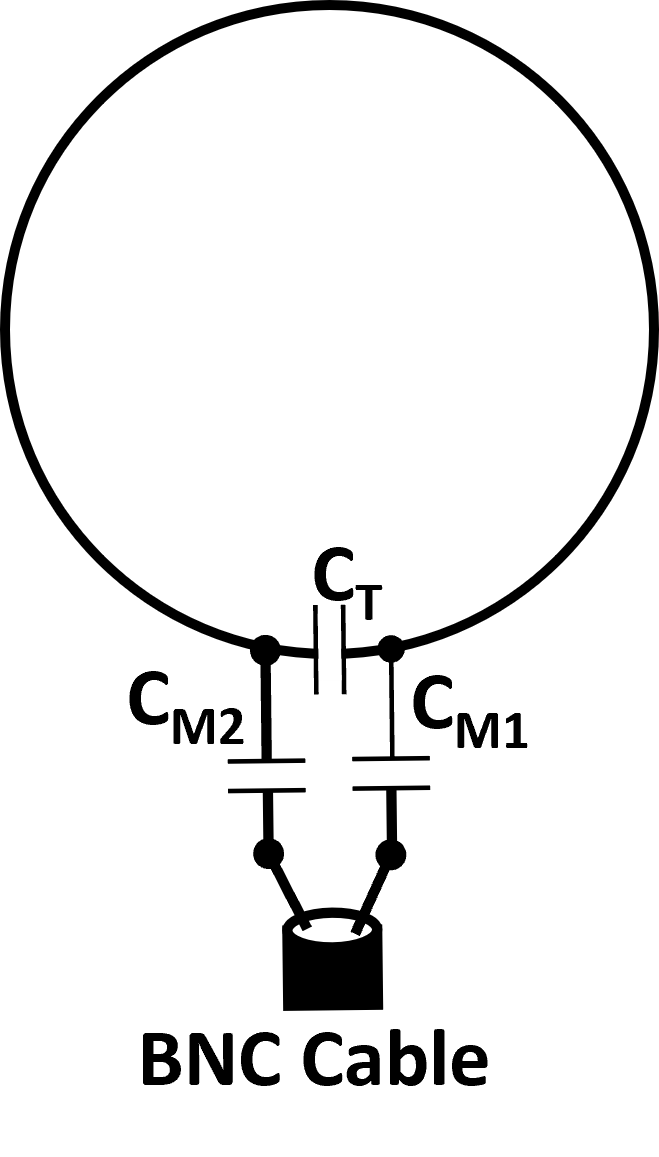
\includegraphics[width=0.3\textwidth]{Figures/Theory/Surface_Coil.png}
    \caption{\textit{Diagram of a typical planar surface coil with circuit elements attached, the coaxial cable attaches to a BNC connector.}}
    \label{fig:theory:Surface}
\end{figure}

The surface coils used for data collection were built for use in Chapter \ref{Chap:Lipid}. The first coil is a small 5 cm coil with two loops of copper wire with tuning capacitance of 173.4 pF and matching 11 pF which is split over both wires of the loop to keep it balanced. The coil is small to maximise the sensitivity to signal from subcutaneous fat in the calf.

\begin{figure}
    \centering
    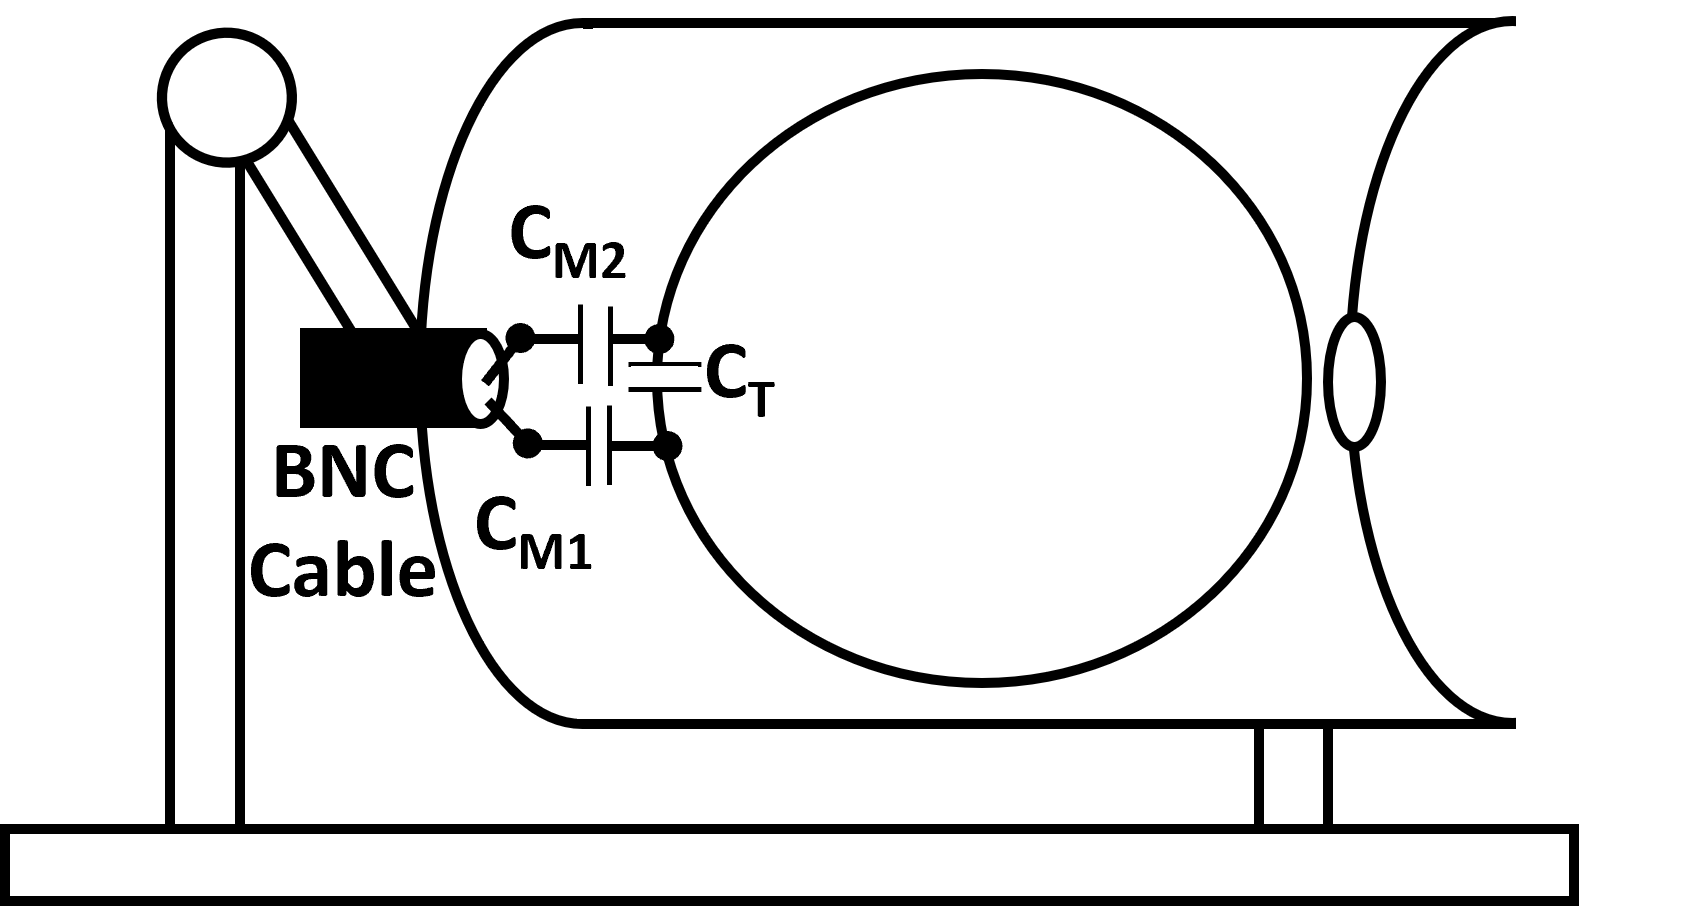
\includegraphics[width=0.7\textwidth]{Figures/Theory/Liver_Coil.png}
    \caption{\textit{Diagram of the surface coil attached to movable housing for scanning of the liver.}}
    \label{fig:theory:Liver}
\end{figure}

The second coil is 12 cm in diameter and again made out of copper wire, and is designed for imaging the liver. This coil is larger so that the penetration dept is large enough to reach the liver. The coil is slightly curved in plane in order for the coil to sit closer to the liver on one side of the abdomen and is mounted to holder so that the coil can be rotated whilst still being attached to the scanner bed.

\begin{figure}
    \centering
    \includegraphics[width=0.9\textwidth]{Figures/Theory/Coil_Pics.png}
    \caption{\textit{Photos of the calf surface coil from two different angles (a \& b) with a photo of the liver surface coil (c), both tuned to the $^2$H Larmor frequency at 3T. The yellow tablets that can be seen in all the photos are vitamin tablets (also known as fiducial markers) used to identify where the coil is in an image.}}
    \label{fig:theory:Pics}
\end{figure}

\subsubsection{Saddle}

\begin{figure}
    \centering
    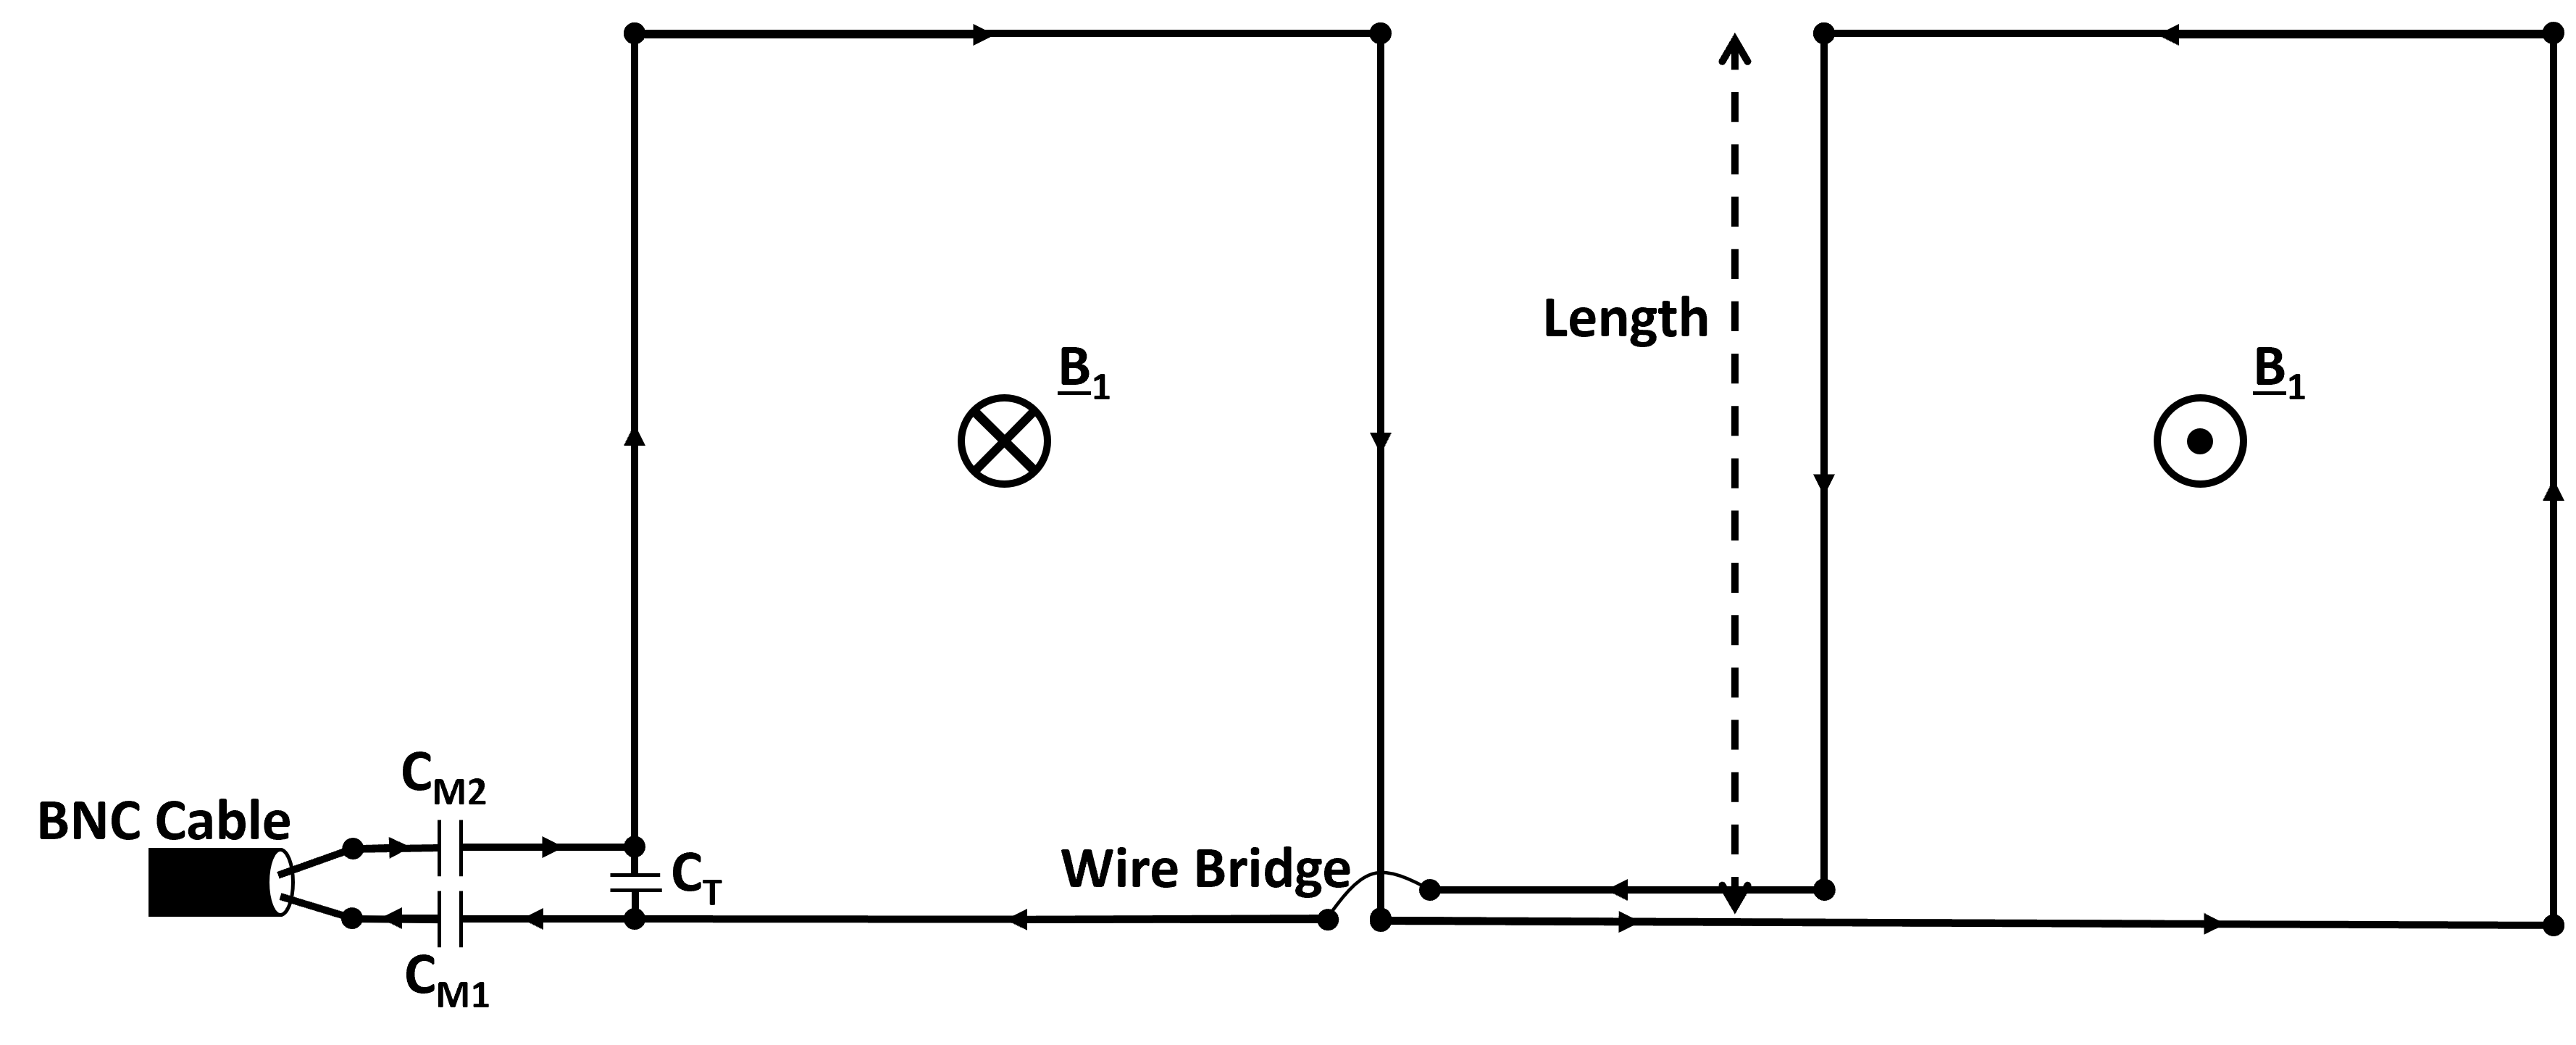
\includegraphics[width=1\textwidth]{Figures/Theory/Planar_Saddle.png}
    \caption{\textit{2D circuit diagram of the saddle coil used for scanning of the calf.}}
    \label{fig:theory:2D_Saddle}
\end{figure}

Volumetric coils such as saddle coils have more homogeneous B$_1$ fields than surface coils and are able to cover a larger volume. A saddle coil derives its name from the fact it has a similar appearance to a horse's saddle, two square loops surround a circular tube with an angular separation. The saddle coil has optimum geometry that has been previously been found which includes the length/diameter between 1 and 2, and an angular width for each coil of $\approx$120$^\circ$ \cite{Ginsberg1970OptimumField,Salmon2006OptimizationImaging}.

\begin{figure}
    \centering
    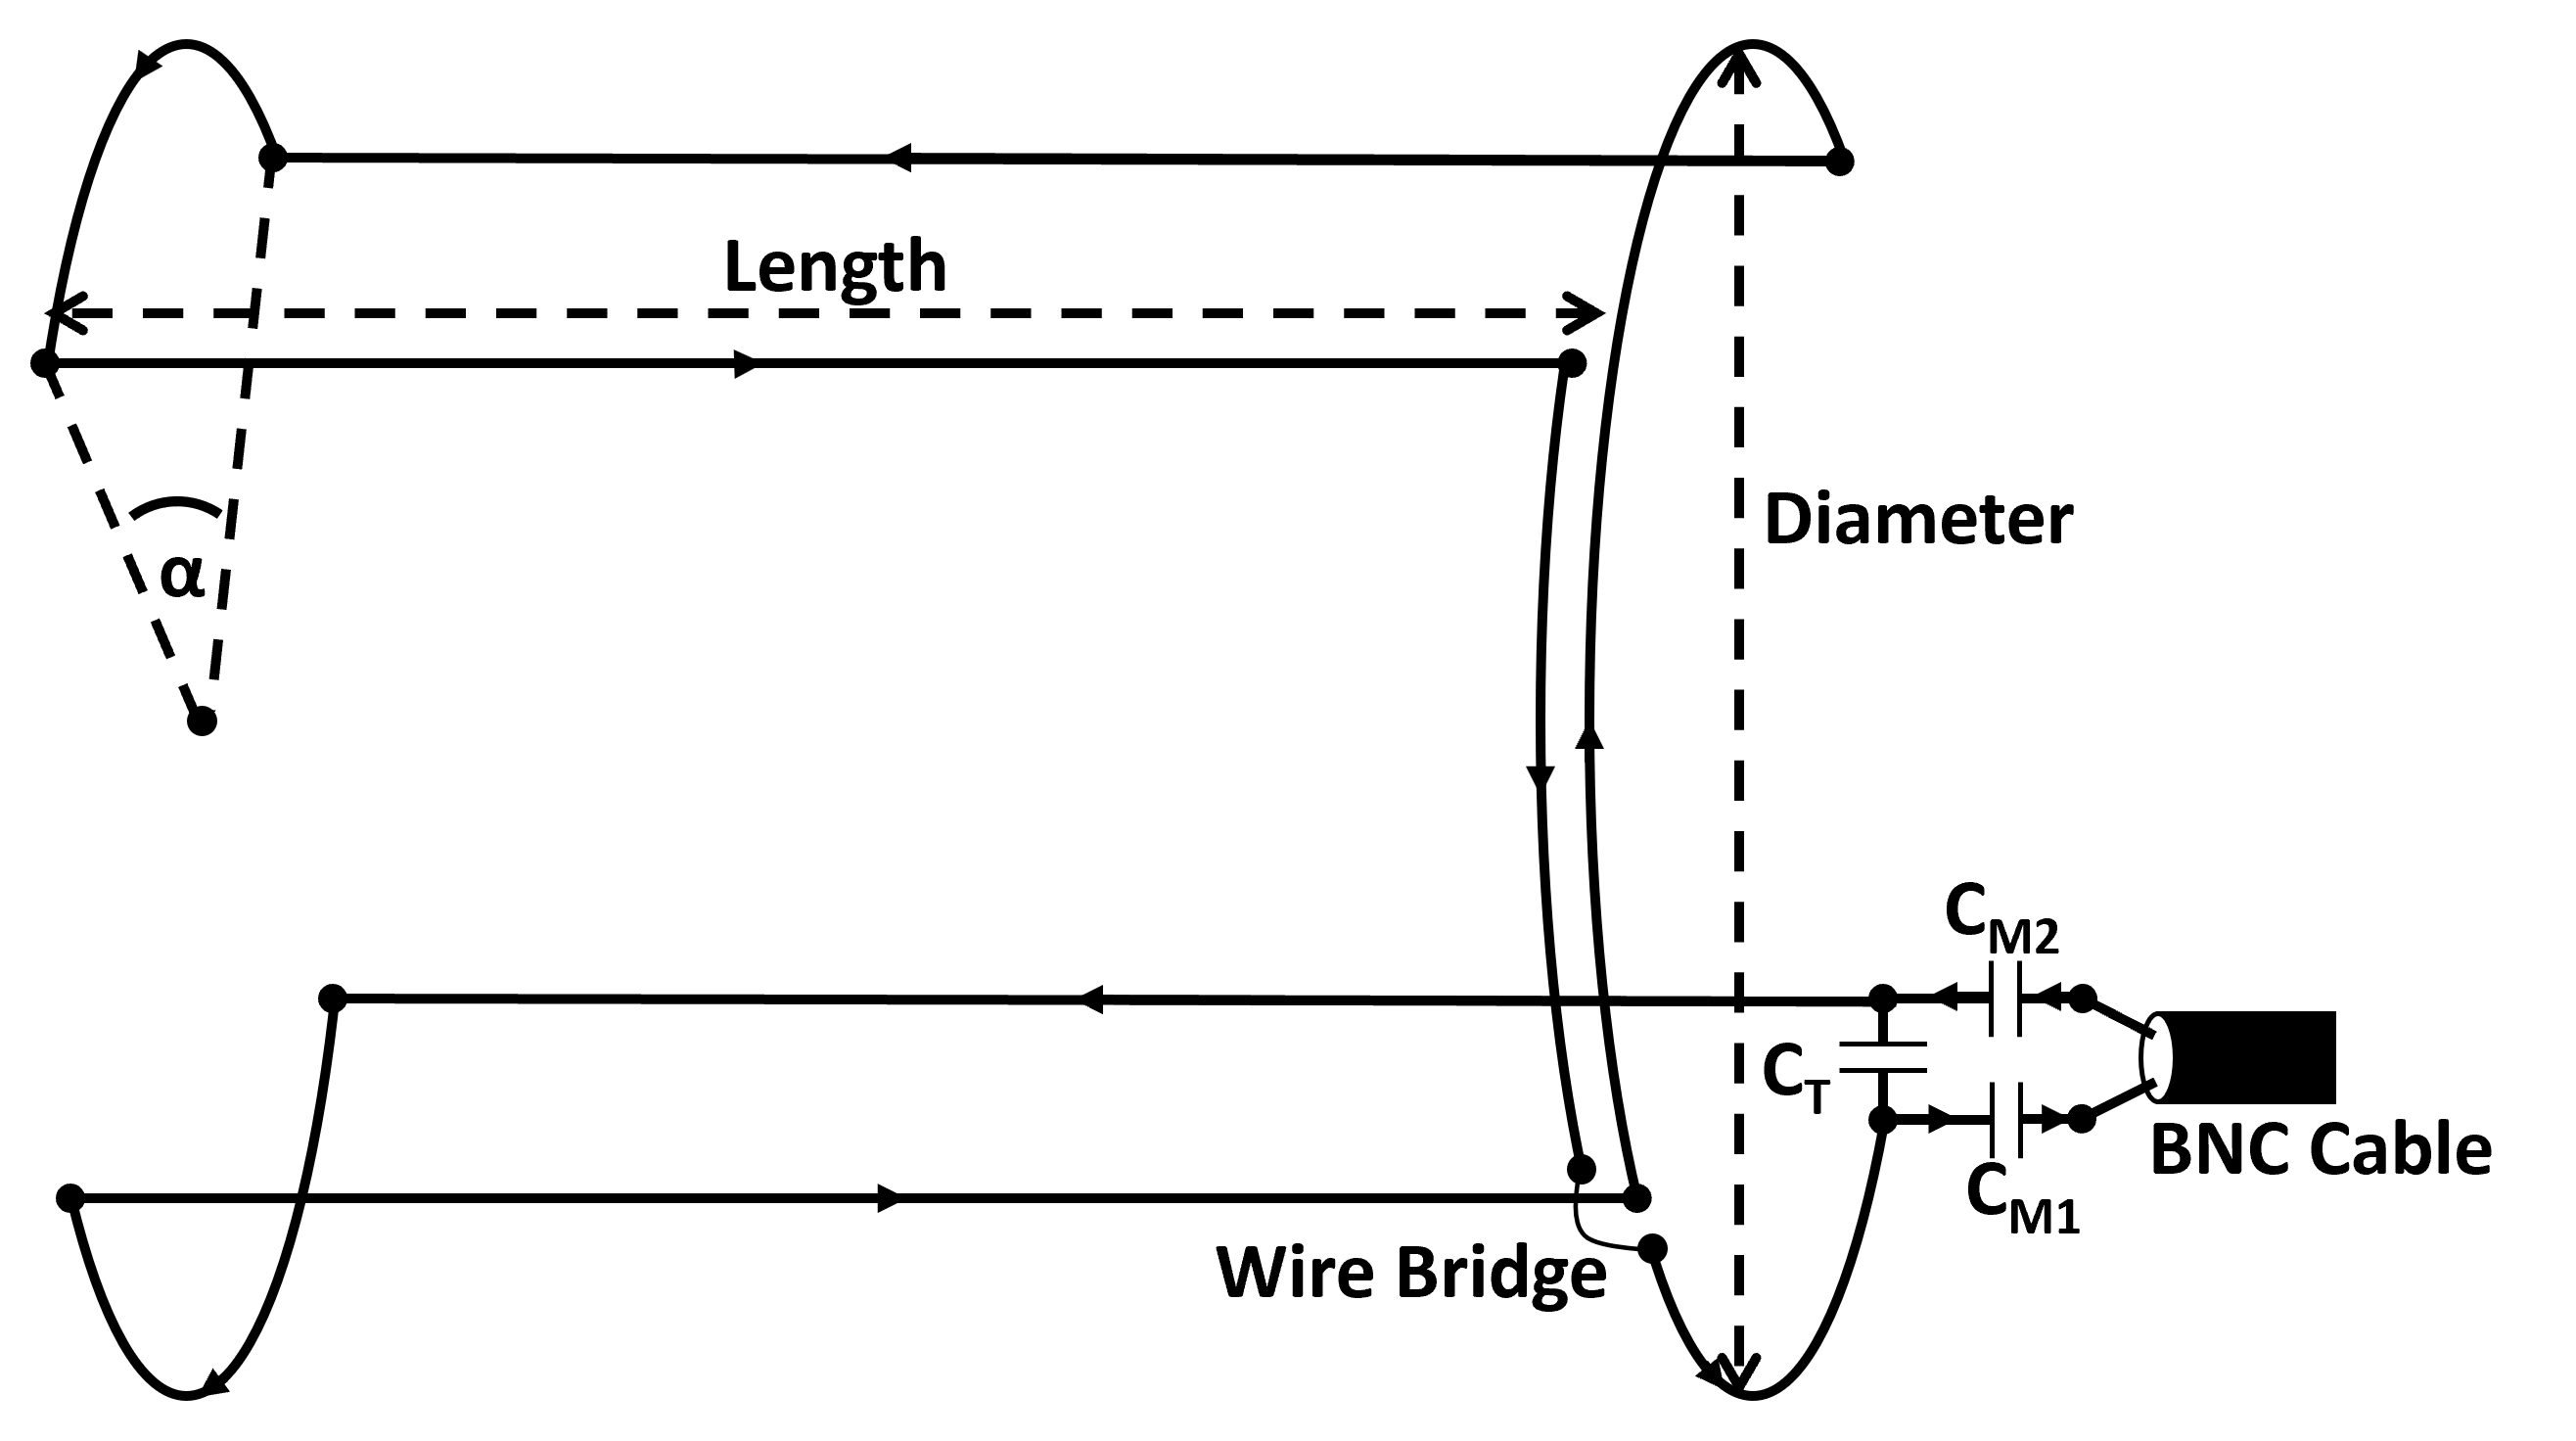
\includegraphics[width=0.8\textwidth]{Figures/Theory/3D_Saddle.png}
    \caption{\textit{3D circuit diagram of the saddle coil used for scanning of the calf.}}
    \label{fig:theory:3D_Saddle}
\end{figure}

The coil built for scanning in Chapter \ref{Chap:Quad} is made from copper tape and has an angular width of 120$^\circ$ a length of 16.8 cm and a diameter of 14.8 cm. Where the copper tape that links the two squares intersects/crosses over an insulated wire is used to avoid a capacitor being created. Also, the wires here run close side by side so that the fields from the opposing currents will cancel. Diagrams of the circuit for the coil are shown in Figs. \ref{fig:theory:2D_Saddle} and \ref{fig:theory:3D_Saddle} with pictures in Fig. \ref{fig:theory:Saddle_pic}. The tuning capacitance is 47.3 pF, the total matching capcitance 8.8 pF.

\begin{figure}
    \centering
    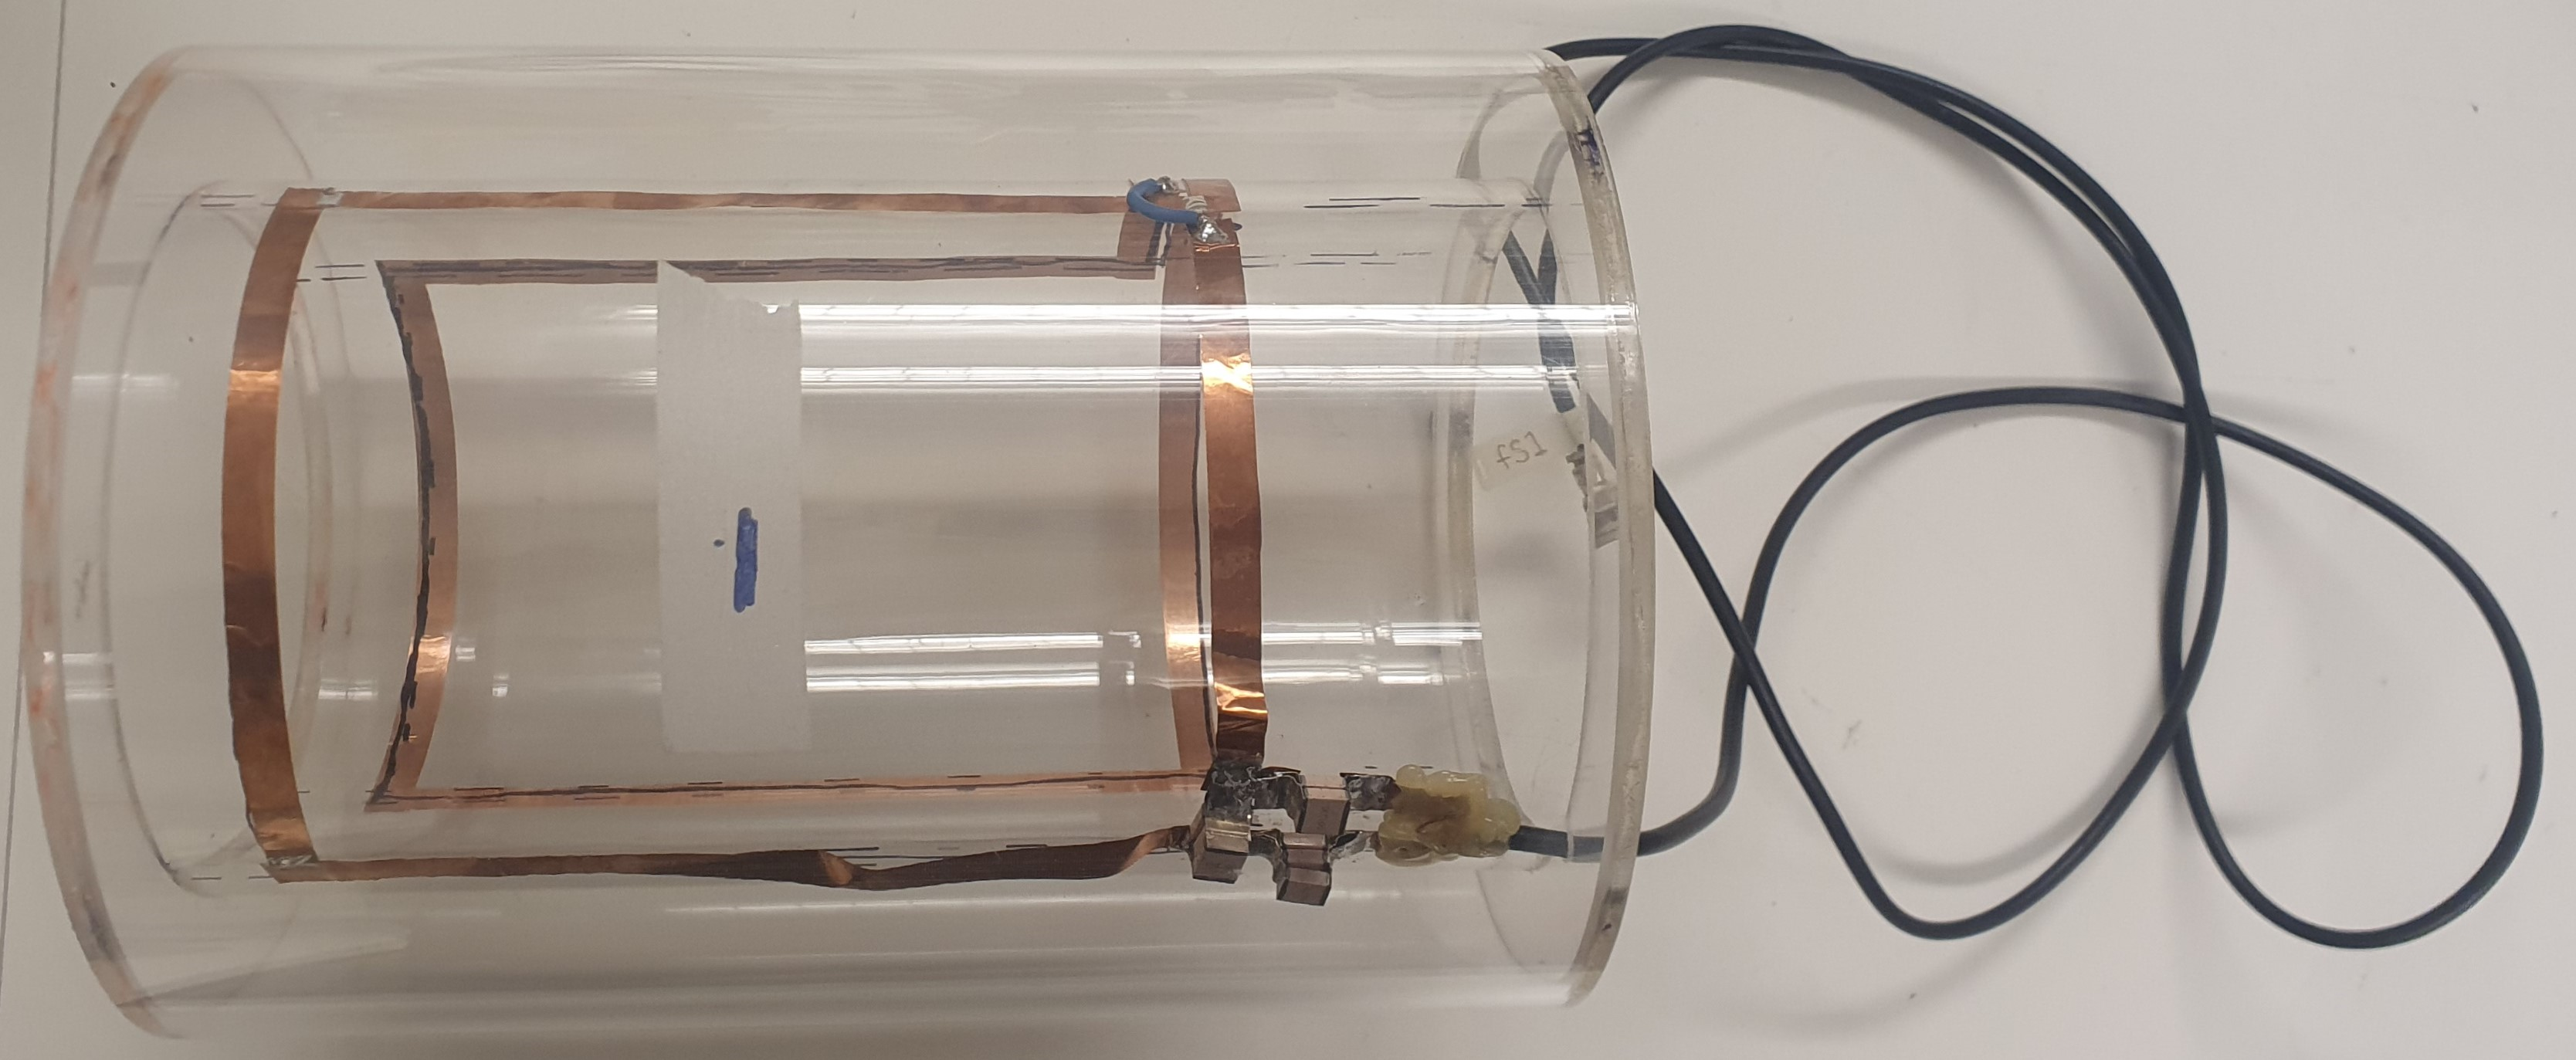
\includegraphics[width=1\textwidth]{Figures/Theory/Saddle_Coil.jpg}
    \caption{\textit{Photo of the saddle coil used to obtain $^2$H data from the calf.}}
    \label{fig:theory:Saddle_pic}
\end{figure}

\subsubsection{Helmholtz coil}

\begin{figure}
    \centering
    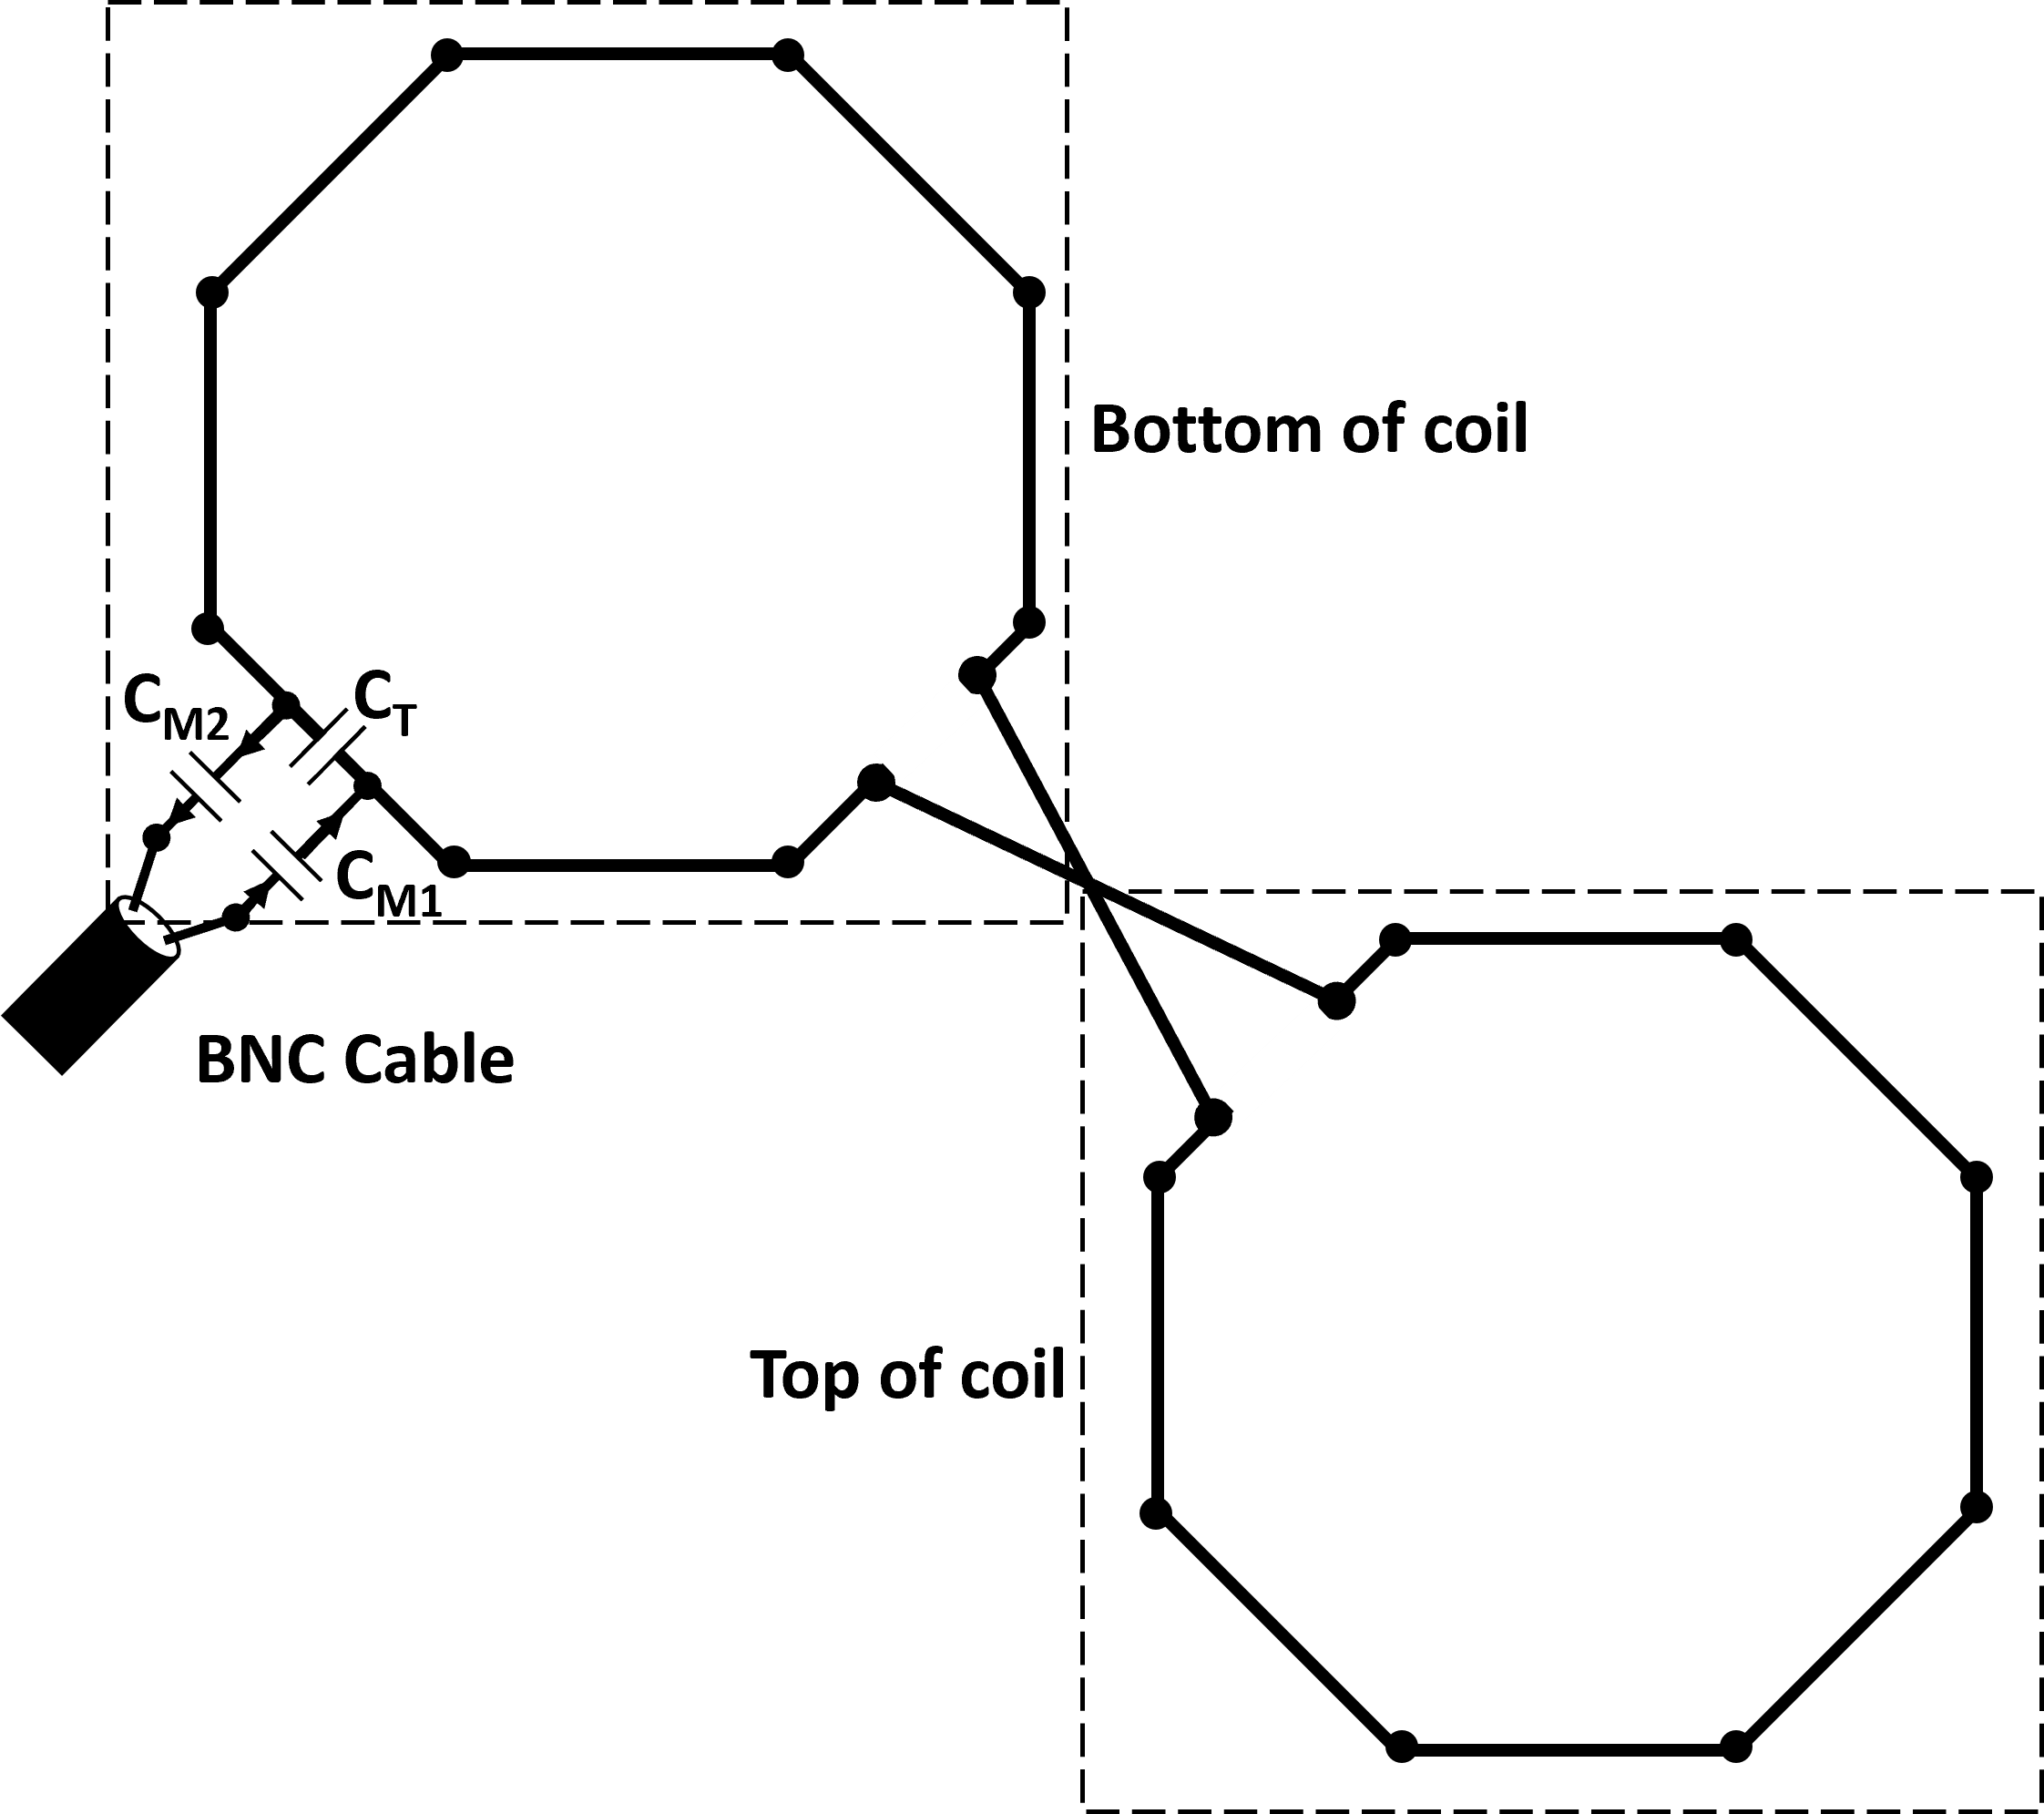
\includegraphics[width=0.8\textwidth]{Figures/Theory/Planar_Helmholtz.png}
    \caption{\textit{2D circuit diagram of the Helmholtz coil used for scanning of the arm.}}
    \label{fig:theory:2D_Helmholtz}
\end{figure}

A Helmholtz coil is similar to to a surface coil in its circuitry. Except a second surface coil is connected to it by two crossing insulated wires, where the current in each flows in opposite directions so that the field flows in the centre of the setup. This creates a homogeneous B$_1$ in between the coils. The Helmholtz coil arrangement was chosen as the scanning is of the arm and needs to be easily movable and a saddle coil would roll/move to much and would be difficult to rotate in the magnet bore.

\begin{figure}
    \centering
    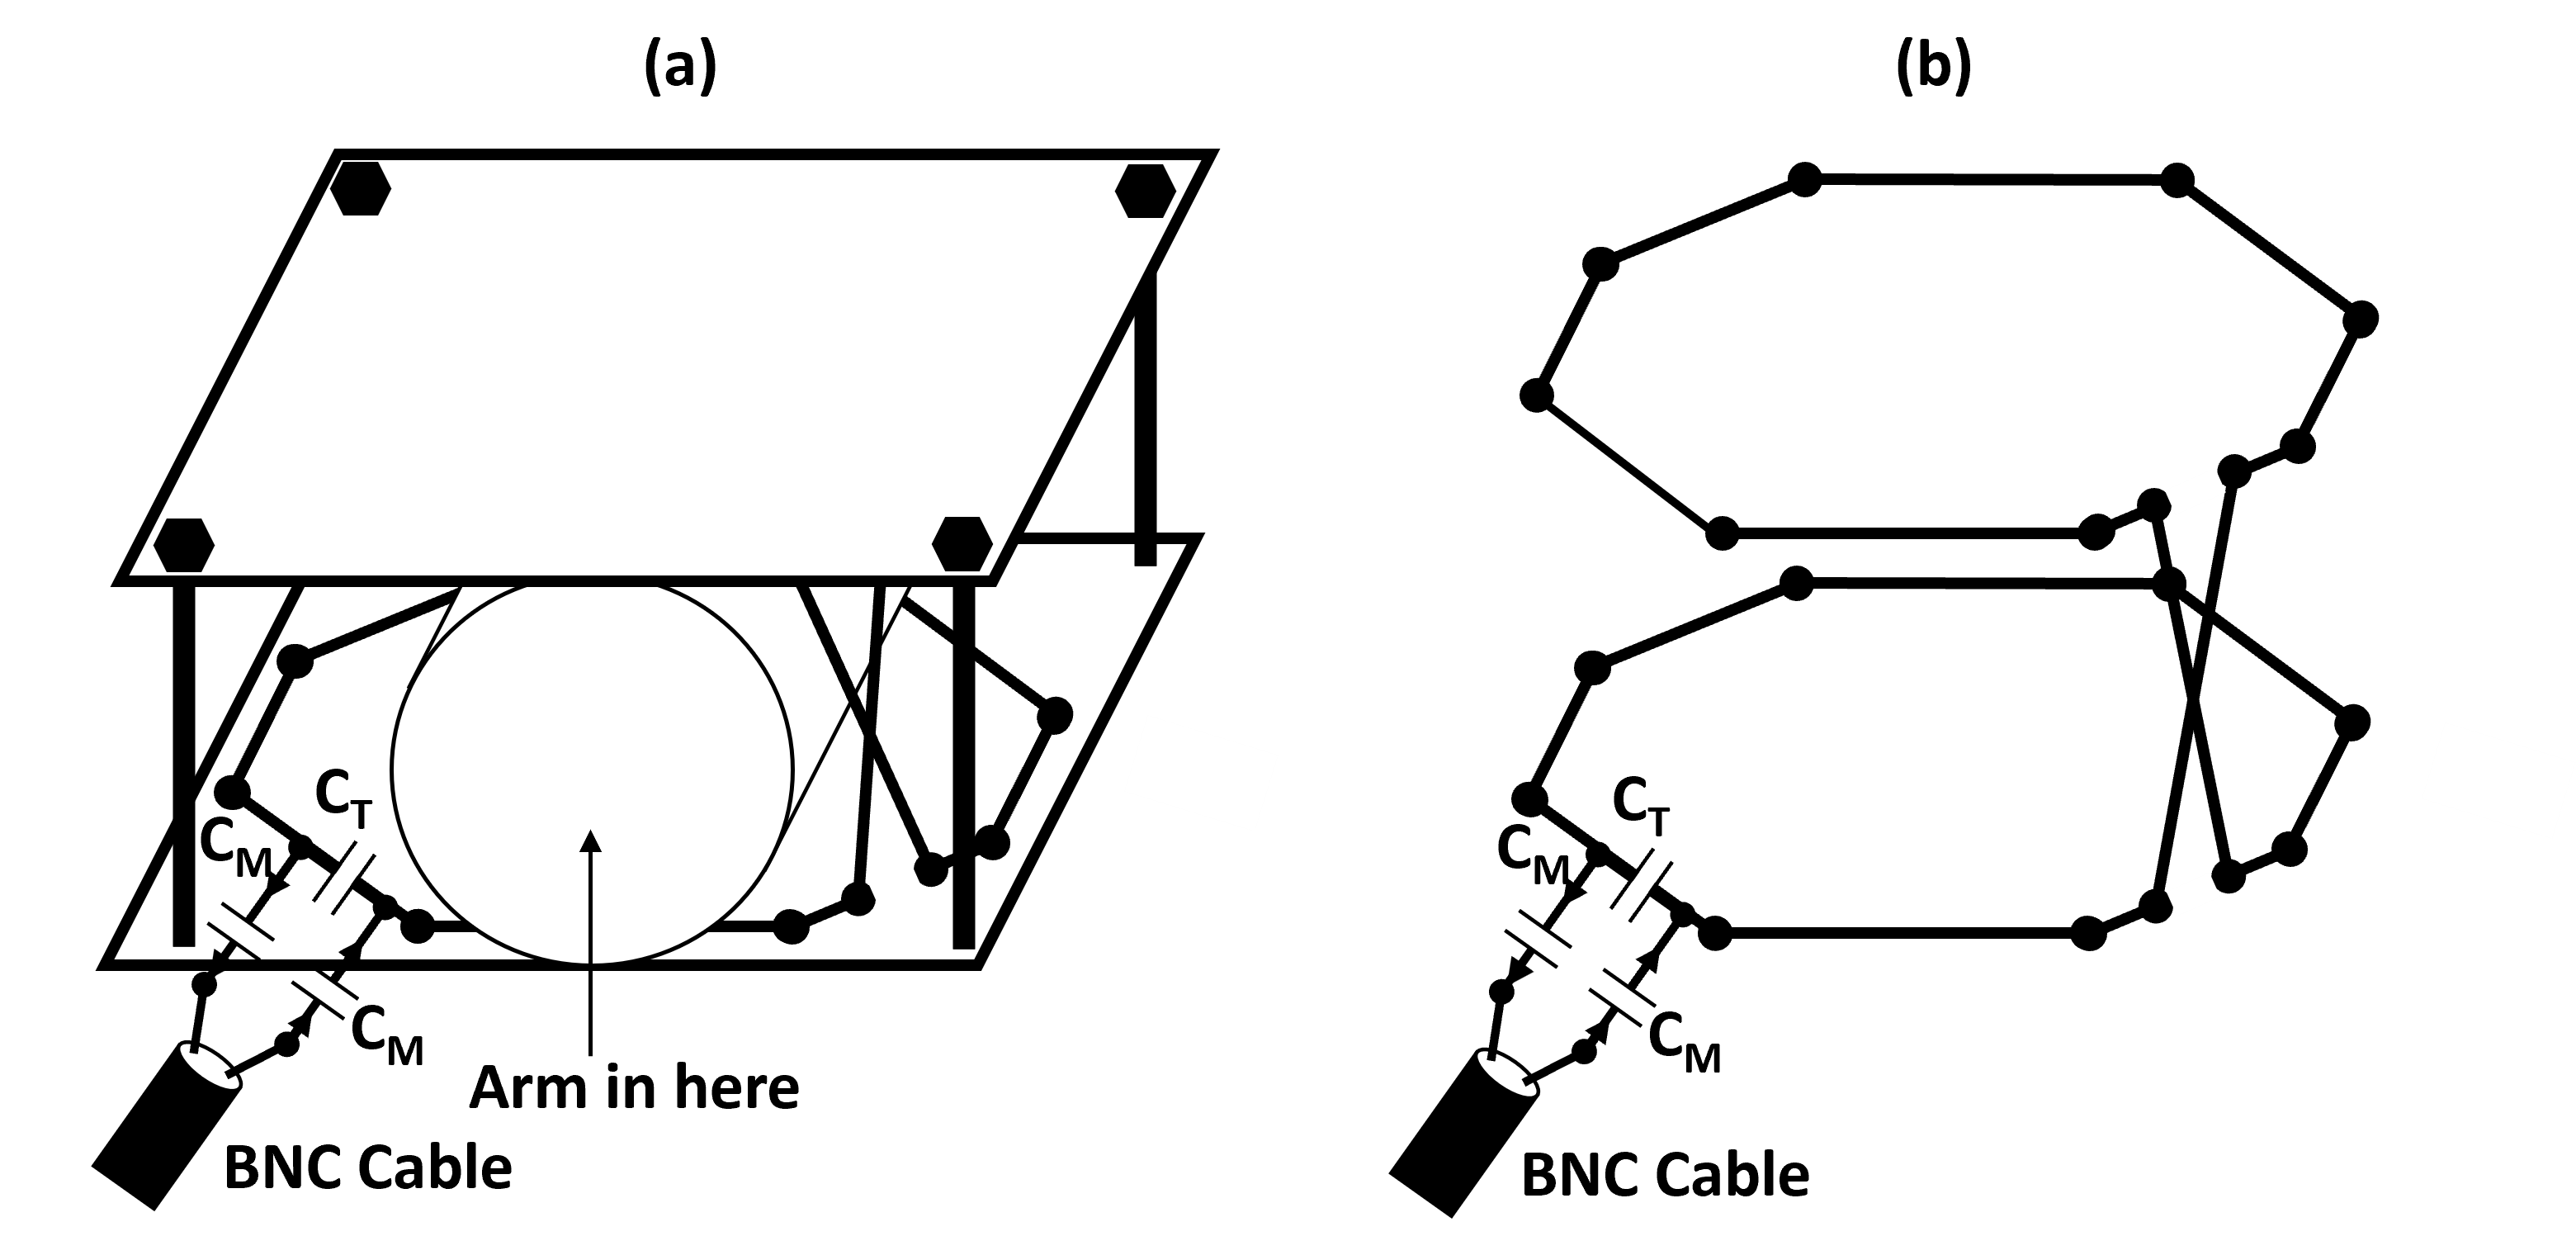
\includegraphics[width=1\textwidth]{Figures/Theory/3D_Helmholtz.png}
    \caption{\textit{3D circuit diagram of the Helmholtz coil used for scanning of the arm with housing (a) and without (b).}}
    \label{fig:theory:3D_Helmholtz}
\end{figure}

The coil setup involves two octagonal loops that are $\approx$14 cm in diameter separated by a 12 cm gap with a tube in the centre to keep the arm in the same position, still and away from the circuit elements. The Tuning capacitance is 73.3 pF and the total matching capacitance is 8.8 pF.

\begin{figure}
    \centering
    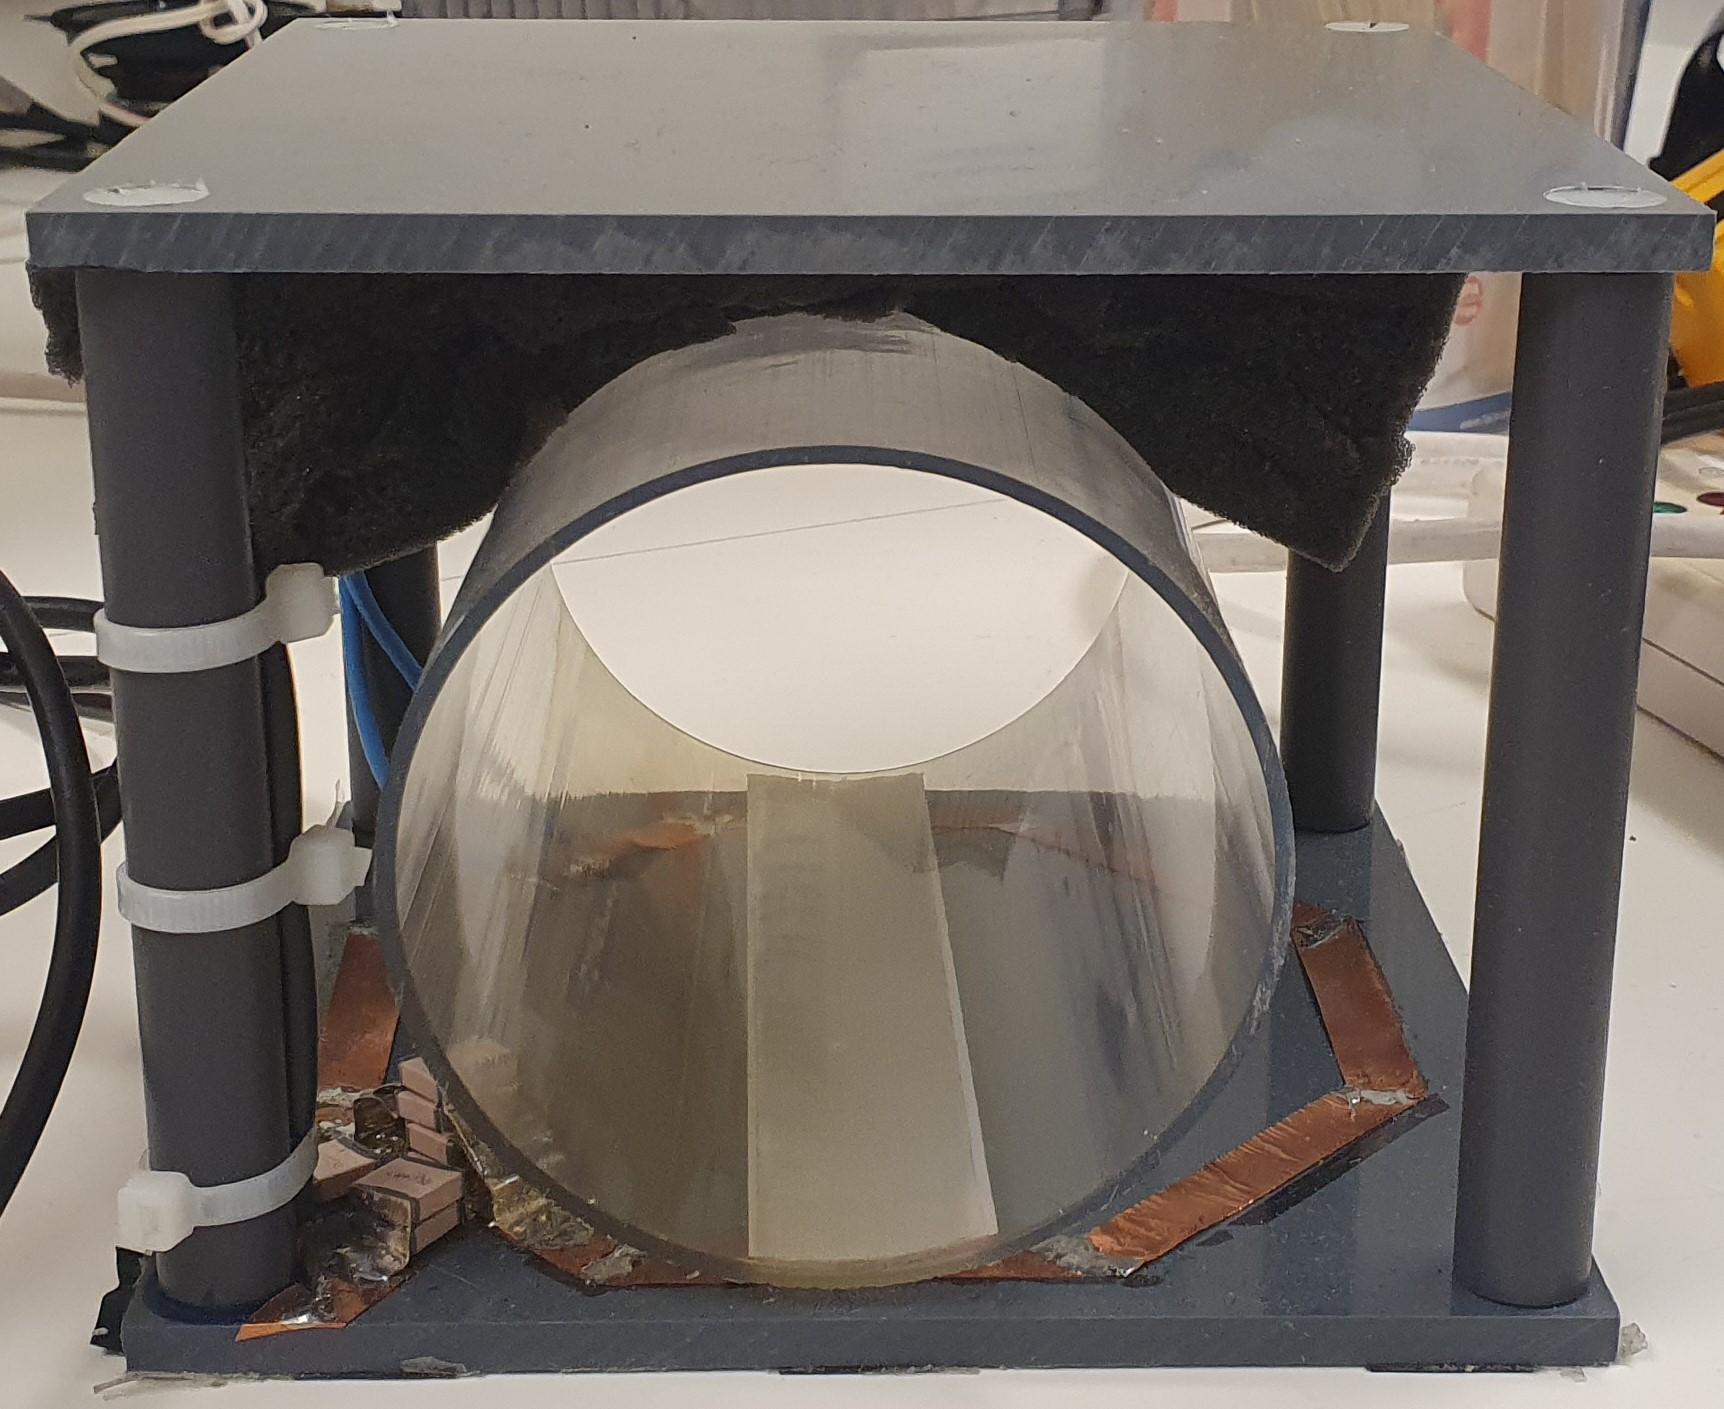
\includegraphics[width=0.8\textwidth]{Figures/Theory/HelmHoltz_Coil.jpg}
    \caption{\textit{Photo of the HelmHoltz coil used to obtain $^2$H data from the arm.}}
    \label{fig:theory:HelmHoltz_pic}
\end{figure}

\newpage
\chapter{Scanning post Heavy Water Loading}
\label{Chap:D2O}

\section{Introduction}

\subsection{Heavy Water Uses}

When most people think of \ac{D$_2$O} they usually think of the the production of nuclear energy and atomic weaponry. However, a very important use of heavy water now is as an isotopic tracer in studies of biochemical processes, such as the assessment of body composition \cite{INTERNATIONALATOMICENERGYAGENCY2011IntroductionSpectrometry} and it is now also often being used to study triglyceride \cite{Strawford2004AdiposeO} and lipid turnover \cite{Wilkinson2017StableFuture}. Studies of lipogenesis in the liver are performed to investigate characteristics of liver disease \cite{Turner2003MeasurementMIDA}. This often involves giving study participants heavy water for a long period of time and then taking blood samples and analysing them \textit{in vitro} using mass spectrometry \cite{Lawitz2022ElevatedPatients, Diraison1997MeasuringTechniques}. The need for blood samples how many measurements can be taken and from where they can be taken, as well as involving patient discomfort. Deuterium magnetic resonance could potentially offer a way to characterise and investigate liver disease non-invasively. 

After drinking \ac{D$_2$O}, rapid exchange occurs between covalent bonded hydrogen atoms and deuterium atoms. This produces an increase in the concentration of \ac{HDO} which is also present at \ac{NA}. This produces an increase in the strength of the \ac{NMR} from $^2$H in water. Covalent bonded hydrogens that exist in the methylene group (-CH$_2$) of fatty acids, can also potentially be replaced by deuterium atoms derived from heavy water, which causes the naturally abundant deuterated fat (CHD) signal to increase. Therefore by using \ac{CSI} over the liver whilst a participant/patient is loaded with heavy water and then tracking the change in concentration of fat/lipid signals over time, lipogenesis could in theory be studied. This approach could be useful in also studying general fat turnover not only in the liver but also in adipose and visceral fat as well. This sort of measurement was previously implemented in healthy and diabetic mice in the 1980's \cite{Brereton1986PreliminarySpectroscopy,Brereton1989TheMice}.

% Removed ', this exchange also occurs with' between increase and Covalent
\subsection{Relaxation Times}

\Ac{DMI} has been shown to be able to provide spatially resolved measurements of metabolite concentrations \cite{Kreis2020MeasuringMRI,Lu2017QuantitativeSpectroscopy}. This makes \ac{DMI} of clinical importance as the metabolite concentrations could potentially be used as bio-markers to assess metabolic disease or tumour aggressiveness, on a patient-to-patient basis. It is straight forward to compare strengths of different metabolite signals, but to work out absolute concentrations you need a reference and also need to account for the different effects of relaxation on the signal strengths. 
% Simply you can calculate molecular abundance by comparing the MR signal of a known abundance to the MR signal of an unknown enrichment, however calculating absolute concentration is more complicated. 

In \ac{DMI} this is performed by comparing the naturally abundant MR signal of \ac{HDO} to the MR signal of other metabolites, along with an attenuation factor which is based on the scan used along with the number of deuterium labels in the metabolite. An estimate of the concentration of \ac{HDO} at \ac{NA} ($\approx$0.0156\%) in the brain is 12.6 mM. This is calculated by multiplying the number of moles in one litre of \ac{D$_2$O} (55.4 Mol) by the water fraction of the brain $\approx$73\% along with the \ac{NA} of $^2$H, remembering to take into account the two $^2$H labels.

The attenuation factor specifically depends on the \ac{TR}, flip angle ($\alpha$) and the T$_1$ of the metabolite in question. Consequently it is of great importance to have an understanding of how T$_1$ changes in different tissues. Previous measurements of \ac{HDO} relaxation times in human participants have used non-localised signals \cite{DeFeyter2018DeuteriumVivo,DeFeyter2021DeuteriumFuture,Ruhm2021DeuteriumResolution} which does not account for the variation of relaxation times across these tissues.

Proton relaxation times have previously been reported in the literature at multiple field strengths for different tissues in the brain \cite{Wright2008WaterOptimization}, and can be used for proton metabolite quantification. Previous measurements of \ac{HDO} relaxation times in human participants used non-localised data \cite{DeFeyter2018DeuteriumVivo, Ruhm2022Dynamic9.4T, Gursan2022ResidualMuscle} which means the variation of relaxation times across specific tissue compartments is not known, making tissue-specific metabolic concentration calculations difficult and unreliable.  

\subsection{Aims}

$^2$H MRI at 7T was used to characterise the \ac{HDO} signals from the human brain in four healthy participants who increased their deuterated water content to $\approx$1.5\% over a six-week period by drinking \ac{D$_2$O}. The heavy water loading was carried out as part of a parallel study into immune cell proteomics. $^2$H MRI and MRS measurements were made on all four participants. This included \ac{MEGE} images acquired at a range of \ac{TR} values, from which T$_1$ and T$_2^*$ relaxation maps were calculated. Co-registration to higher resolution $^1$H images allowed T$_1$ and T$_2^*$ relaxation times of deuterium in \ac{HDO} in \ac{CSF}, \ac{GM}, and \ac{WM} to be reported. For two of the participants, $^2$H \ac{MRI}/\ac{MRS} data was also acquired during the initial $\sim$eight-hour loading period to track the time-course of $^2$H enrichment within the brain \cite{Cocking2023DeuteriumDosing}. The work described in this chapter formed the basis of the peer-reviewed paper 'Deuterium brain imaging at 7T during D$_2$O dosing' published in the journal 'Magnetic Resonance in Medicine' \cite{Cocking2023DeuteriumDosing}.

%When creating an MRS/MRI scan it is important to be aware of the transverse relaxation time (T$_{2}^{*}$) of the tissue and metabolite you are investigating as this gives excellent insight on to how the signal is decaying and allows you to choose appropriate TR's and $\alpha$'s for the scan.

\section{Methodology}

Six healthy participants took part in this $^2$H-imaging sub-study which was approved by the local institutional ethics committee and the volunteers gave informed consent. Two of the participants were scanned during a set-up phase in which we established the feasibility of $^2$H imaging and identified favourable imaging parameters. Here, I report data from four participants (A - D) who were subsequently scanned using the optimised imaging protocols. All scanning was performed on a 7T Philips Achieva scanner (Philips Healthcare, Amsterdam, The Netherlands), operating at 45.8 MHz for $^2$H and 298 MHz for $^1$H. A 26.4 cm inner diameter, dual-tuned $^1$H/$^2$H birdcage coil (Rapid Biomedical) was used for deuterium measurements, while the standard 32-channel Rx/2-channel Tx head coil (Nova Medical) was used for acquiring anatomical $^1$H images.  

The proteomics study required an initial loading regime in which the targeted enrichment was built up in around 8 hours. This was achieved by participants drinking between 12 and 16, $\sim$50 ml doses of 70\% D$_2$O/30\% H2O every $\sim$30 minutes, with the total amount of \ac{D$_2$O} consumed adjusted according to the participant’s body weight, so that an enrichment of around 1.5\% was produced. The participants subsequently drank $\sim$50 ml of \ac{D$_2$O} each morning over the six-week study period to maintain a $\sim$1.5\% enrichment. Similar enrichment levels and durations have been used in recent studies \cite{Robinson2011Long-termSupplementation, Burger2017LeukemiaIbrutinib, Loomba2019DiscoveryLabeling} with no adverse events reported. However some participants experienced a brief period of dizziness during the initial loading phase due to the rapid rise in body water enrichment \cite{Robinson2011Long-termSupplementation}. 

% Not included as data not included: 'Saliva samples were also collected from participants at regular intervals during the study and analyzed using gas chromatography–mass spectrometry (GCMS)'\cite{Yang1998AssaySpectrometry}.  

\subsection{Initial Loading}

Two of the participants (A and B) were scanned during the initial 8-hour loading period to monitor the time-course of changes in the concentration of $^2$H in the brain. A scanning protocol of $\sim$15 minutes’ duration was performed before dosing and then again after 30, 90, 150, 210, 270, 360, 420 and 540 minutes. The protocol comprised, a $^1$H scout scan for planning, followed by acquisition of $^2$H pulse-acquire spectra from the whole head and then from a 2-cm-thick axial slice positioned over the lateral ventricles. Both used the following scan parameters: $\alpha$ = 90$^\circ$, 2048 samples, \ac{BW} = 3000 Hz, repetition time TR = 1 s and 64 averages (acquisition time T$_\text{scan}$ = 64 s). We then acquired axial, \ac{MEGE} $^2$H images (20 averages, T$_\text{scan}$ = 453s, \ac{FOV} = 288x288x80 mm$^3$, 6x6x10 mm$^3$ voxels, $\alpha$ = 33$^\circ$, \ac{TR} = 62 ms, five echoes, \ac{TE} = 8.9 ms and $\Delta$\ac{TE} = 8.4 ms. Axial $^1$H \ac{GE} images (T$_\text{scan}$ = 232 s, 32 slices, \ac{FOV} = 288x288x80 mm$^3$, 3x3x2.5 mm$^3$ voxels, \ac{TE} = 5.9 ms, \ac{TR} = 39 ms) were also acquired. The scanning protocol was repeated 17 days after the initial loading to obtain comparative data at steady-state enrichment. 

The spectroscopy measurements made before loading provided an estimate of the signal from naturally abundant deuterium in water: scaling subsequent measurements then allowed the absolute \ac{HDO} concentration to be estimated at each time-point. The \ac{HDO} concentration in the body was also estimated from the ratio of the total imbibed \ac{D$_2$O} volume to an estimate of total body water using the participant’s height, weight, age and gender \cite{Watson1980TotalMeasurements}. The temporal variation of \ac{HDO} concentration in the brain was monitored by plotting the amplitude of the single peak in each non-selective and selective spectrum against the time since the first heavy water dose. The peak amplitude was obtained by fitting the complex data to a Lorentzian line shape in the frequency domain using non-linear least squares fitting. 

\begin{figure}[H]
    \centering
    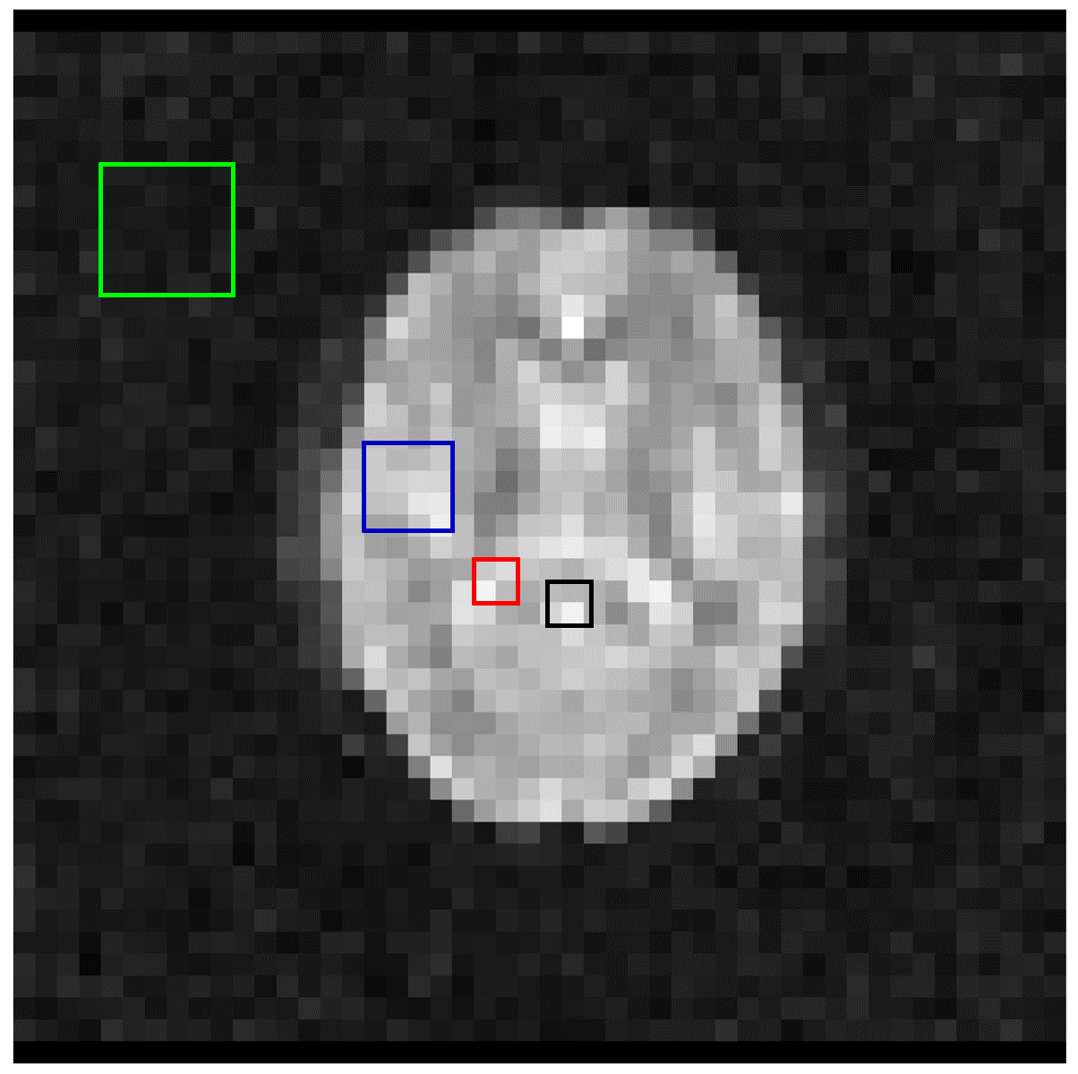
\includegraphics[width=0.7\textwidth]{Figures/D2O/ROI.png}
    \caption{\textit{Regions of interest used for following the time-course of signal change during \ac{D$_2$O} loading. Black = \ac{SC}; Red = lateral ventricle; Blue = brain (\ac{GM}, \ac{WM} and \ac{CSF}); Green = background noise.}}
    \label{fig:D2O:ROI}
\end{figure}

We used the image data to track the changes in $^2$H signal from different tissue compartments. The $^2$H images acquired at each time-point were summed over the five echoes to form a single image data set. Then using both the $^2$H and $^1$H images, \ac{ROI} were formed for a background region, general brain tissue, the lateral ventricles and for a region of high signal intensity thought to arise from blood vessels and \ac{CSF} in the \ac{SC}. Examples of the \ac{ROI}s used are shown in Fig. \ref{fig:D2O:ROI}. The signal intensity in each region was plotted against time from the first heavy water dose. The \ac{SNR} in images acquired before loading was too low to make good estimates of \ac{NA} signal strength, so values were normalized to the signal measured in the superior cistern \ac{ROI} at the last time point of the initial loading period. All analysis was performed using MATLAB (Release 2020b, The MathWorks, Inc., Natick, MA, United States).

\subsection{Relaxation Time Measurements}
\label{Chap:D2O:Relaxation}

$^2$H relaxation times for water in \ac{CSF}, \ac{GM}, and \ac{WM} were calculated from data acquired during the six-week loading period using the dual-tuned $^2$H/$^1$H coils. In each imaging session, $^2$H 3D sagittal \ac{MEGE} images were acquired (voxels = 6 x 6 x 10 mm$^3$, \ac{FOV} = 288 x 288 x 240 mm$^3$, slices = 24) at a range of \ac{TR} values, along with $^1$H 3D \ac{MEGE} images (voxels = 3 x 3 x 5 mm$^3$, \ac{FOV} = 288 x 288 x 240 mm$^3$, slices = 48, 15 \ac{TE}s with TE$_1$ = 2.5 ms, $\Delta$TE = 2.34 ms, and TR = 41 ms). 

$^2$H \ac{MEGE} data from Participants A and B were acquired with five echoes (\ac{TE} = 4.3 ms, $\Delta$TE = 8.4 ms), $\alpha$ = 60° and \ac{TR} = 68, 136, 272 and 544 ms, with 8, 4, 2 and 1 averages so that T$_\text{scan}$ = 487 s for each image. $^2$H \ac{MEGE} data from participants C and D was acquired with six echoes (\ac{TE} = 4.3 ms; $\Delta$TE = 8.4 ms) and one additional \ac{TR} value (TR = 816 ms; T$_\text{scan}$ = 730 s; 1 average). 
The number of \ac{TE} and \ac{TR} values were increased for participants C and D to improve fitting quality. The $^2$H scanning sessions were performed twice on Participants C and D.

In a separate scanning session using the Nova coil, $^1$H  \ac{MPRAGE} images (0.7 mm resolution) and $^1$H 3D \ac{MEGE} images (3x3x5 mm$^3$ voxels, 15 echo times, TE$_1$ = 2.5 ms, $\Delta$TE = 2.57 ms, and \ac{TR} = 41 ms) were acquired from each participant. These images were used for image segmentation and estimation of the $^1$H T$_2^*$ values. 

For calculation of $^2$H relaxation time maps, we first estimated the variation of flip angle ($\alpha$) over the image volume by summing the images across \ac{TE}s, at each \ac{TR}, and then fitting the resulting image data voxel-wise to a saturation recovery curve (i.e., fitting signal variation with \ac{TR} for $\alpha$, R$_1$, and signal amplitude). The resulting flip-angle maps were smoothed by averaging over 5 x 5 x 5 voxel neighbourhood and the $\alpha$-values used as a fixed variable in dual-fitting the variation in signal intensity S$_{i,j}$ across TR$_i$ and TE$_j$  values. 
\begin{equation}
     \sum_{i=1}^{n_{\text{TR}}}\sum_{j=1}^{n_{\text{TE}}}\left|\frac{A\sin{\alpha}(1-\exp(-R_1 \text{TR}_i)}{1-\cos{\alpha}\exp(-R_1 \text{TR}_i)}*\exp(-R_2^*\text{TE}_j) - S_{i,j}\right|^2
     \label{eqn.min}
\end{equation}
This involved minimisation of Eq. \ref{eqn.min} using the Matlab fmincon command, $^1$H R$_2^*$ maps were obtained by similar fitting to the exponential signal decay with \ac{TE} in the $^1$H \ac{MEGE} data acquired using the Nova coil.

To evaluate the relaxation times in different compartments, we segmented the $^1$H \ac{MPRAGE} data (FSL FAST \cite{Zhang2001SegmentationAlgorithm}) and transformed the resulting \ac{GM}, \ac{WM} and \ac{CSF} masks to the space of the $^2$H relaxation time maps. Following brain extraction (FSL BET \cite{Smith2002FastExtraction}) and bias field correction, an affine matrix was obtained from image co-registration (FSL FLIRT \cite{Jenkinson2001AImages,Jenkinson2002ImprovedImages}) which transformed the $^1$H \ac{MEGE} data acquired using the dual-tuned coil to the $^1$H \ac{MEGE} Nova Medical coil data, along with an affine matrix for the $^1$H \ac{MEGE} to \ac{MPRAGE} transformation. Image co-registration was linear, with six degrees of freedom and used the correlation ratio cost function. The \ac{MEGE} data were summed across echoes and repetition times before co-registration.

The brain-extracted \ac{MPRAGE} image was segmented to create binary masks for \ac{GM}, \ac{WM} and \ac{CSF} using FSL FAST \cite{Zhang2001SegmentationAlgorithm}. These masks were then transformed to the $^2$H space using the previously obtained affine matrices and the outer regions of the CSF mask were manually removed so that the majority of the CSF mask come from the lateral ventricles. The new masks were binarized at a value of 0.6 for each tissue to ensure that each mask contained at least 25 voxels for averaging. The binarized masks were applied to the relaxation maps for calculation of mean relaxation times for \ac{CSF}, \ac{GM} and \ac{WM}.

\section{Results}
\subsection{Loading}

\begin{figure}[H]
    \centering
    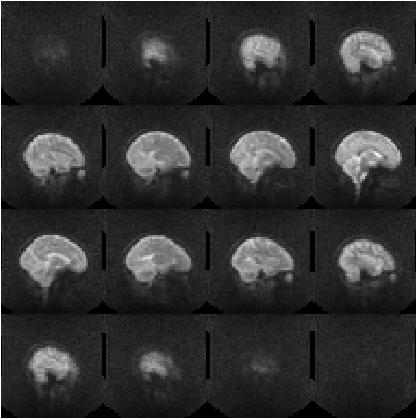
\includegraphics[width=0.7\textwidth]{Figures/D2O/Sag_Full.png}
    \caption{\textit{3D MEGE $^2$H image data from Participant C. Images produced by summing over six TE values and five TR values. Voxel size=6 × 6 × 10 mm$^3$, FOV=288 × 288 mm$^2$, T$_\textrm{scan}=485$ s for each TR value.}}
    \label{fig:D2O:Sag_Full}
\end{figure}

Figure \ref{fig:D2O:Sag_Full} shows example $^2$H 3D sagittal images obtained by summing the $^2$H \ac{MEGE} data for a single (fully loaded) subject over \ac{TE} and \ac{TR} values, during the steady-state loading period. The resulting images, which predominantly show T$_2^*$ contrast, clearly depict the brain anatomy and have a similar appearance to T$_2^*$-weighted, $^1$H images. The \ac{CSF} in the ventricles and at the cortical surface appears hyperintense, while regions of white matter where there is little partial-voluming with \ac{CSF}, such as in the corpus callosum, appear hypointense. Figure \ref{fig:D2O:TR_TE} shows the variation of image intensity with TE and TR in a central sagittal slice. The slower T$_2^*$ decay of the CSF signal compared with that of the \ac{GM} and \ac{WM} signals is evident, along with the signal saturation at reduced \ac{TR}, and the reduction of contrast at low \ac{TE} and \ac{TR} values. In Fig. \ref{fig:D2O:Load}, example $^2$H images acquired from participants A and B at different dosage times during the initial loading process are shown. As dosage increases, so does the overall \ac{SNR}. The \ac{ROI}s that were used to analyse the loading in different brain tissues are outlined in Fig. \ref{fig:D2O:ROI} (for participant A). Since the background \ac{MEGE} image is obtained after the final dose for Subject A the tissues being segmented are easily discerned in the $^2$H images. However, for the lower dosage images this is not the case, which is why the \ac{ROI}’s are defined on the anatomical $^1$H image. 

\begin{figure}[H]
    \centering
    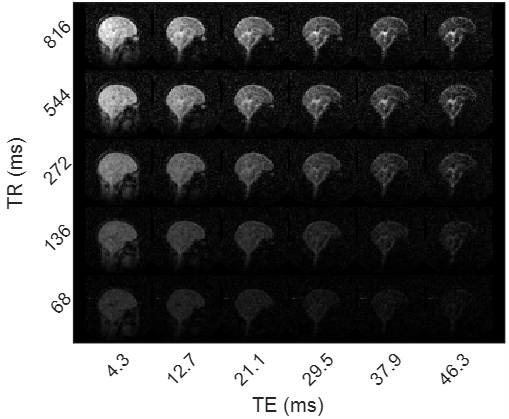
\includegraphics[width = 0.7\textwidth]{Figures/D2O/TR_TE.png}
    \caption{\textit{3D MEGE $^2$H image from one slice from Participant D. Images are displayed with TE value varying horizontally and TR-value varying vertically. Voxel size=6 × 6 × 10 mm$^3$, FOV=288 × 288 mm$^2$, T$_\textrm{scan}=485$ s for each \ac{TR} value.}}
    \label{fig:D2O:TR_TE}
\end{figure}

The qualitative increase in signal during the loading period in Fig. \ref{fig:D2O:Load} is shown more quantitatively in Fig. \ref{fig:D2O:Bulk}, which plots the $^2$H concentration time course obtained from the spectroscopy data, along with the steady-state values measured after 17 days of loading. The average signal from each \ac{ROI} during loading is shown in Fig. \ref{fig:D2O:ROI_Graph} scaled to the signal measured in the \ac{SC} at the last time point, in the brain along with the steady-state values measured after 17 days of loading. Plotted values from Figs. \ref{fig:D2O:Bulk} and \ref{fig:D2O:ROI_Graph} also show the $^2$H concentration estimated from the cumulative D$_2$O dose and estimated total body water volume, for comparison. 

\begin{figure}[H]
    \centering
    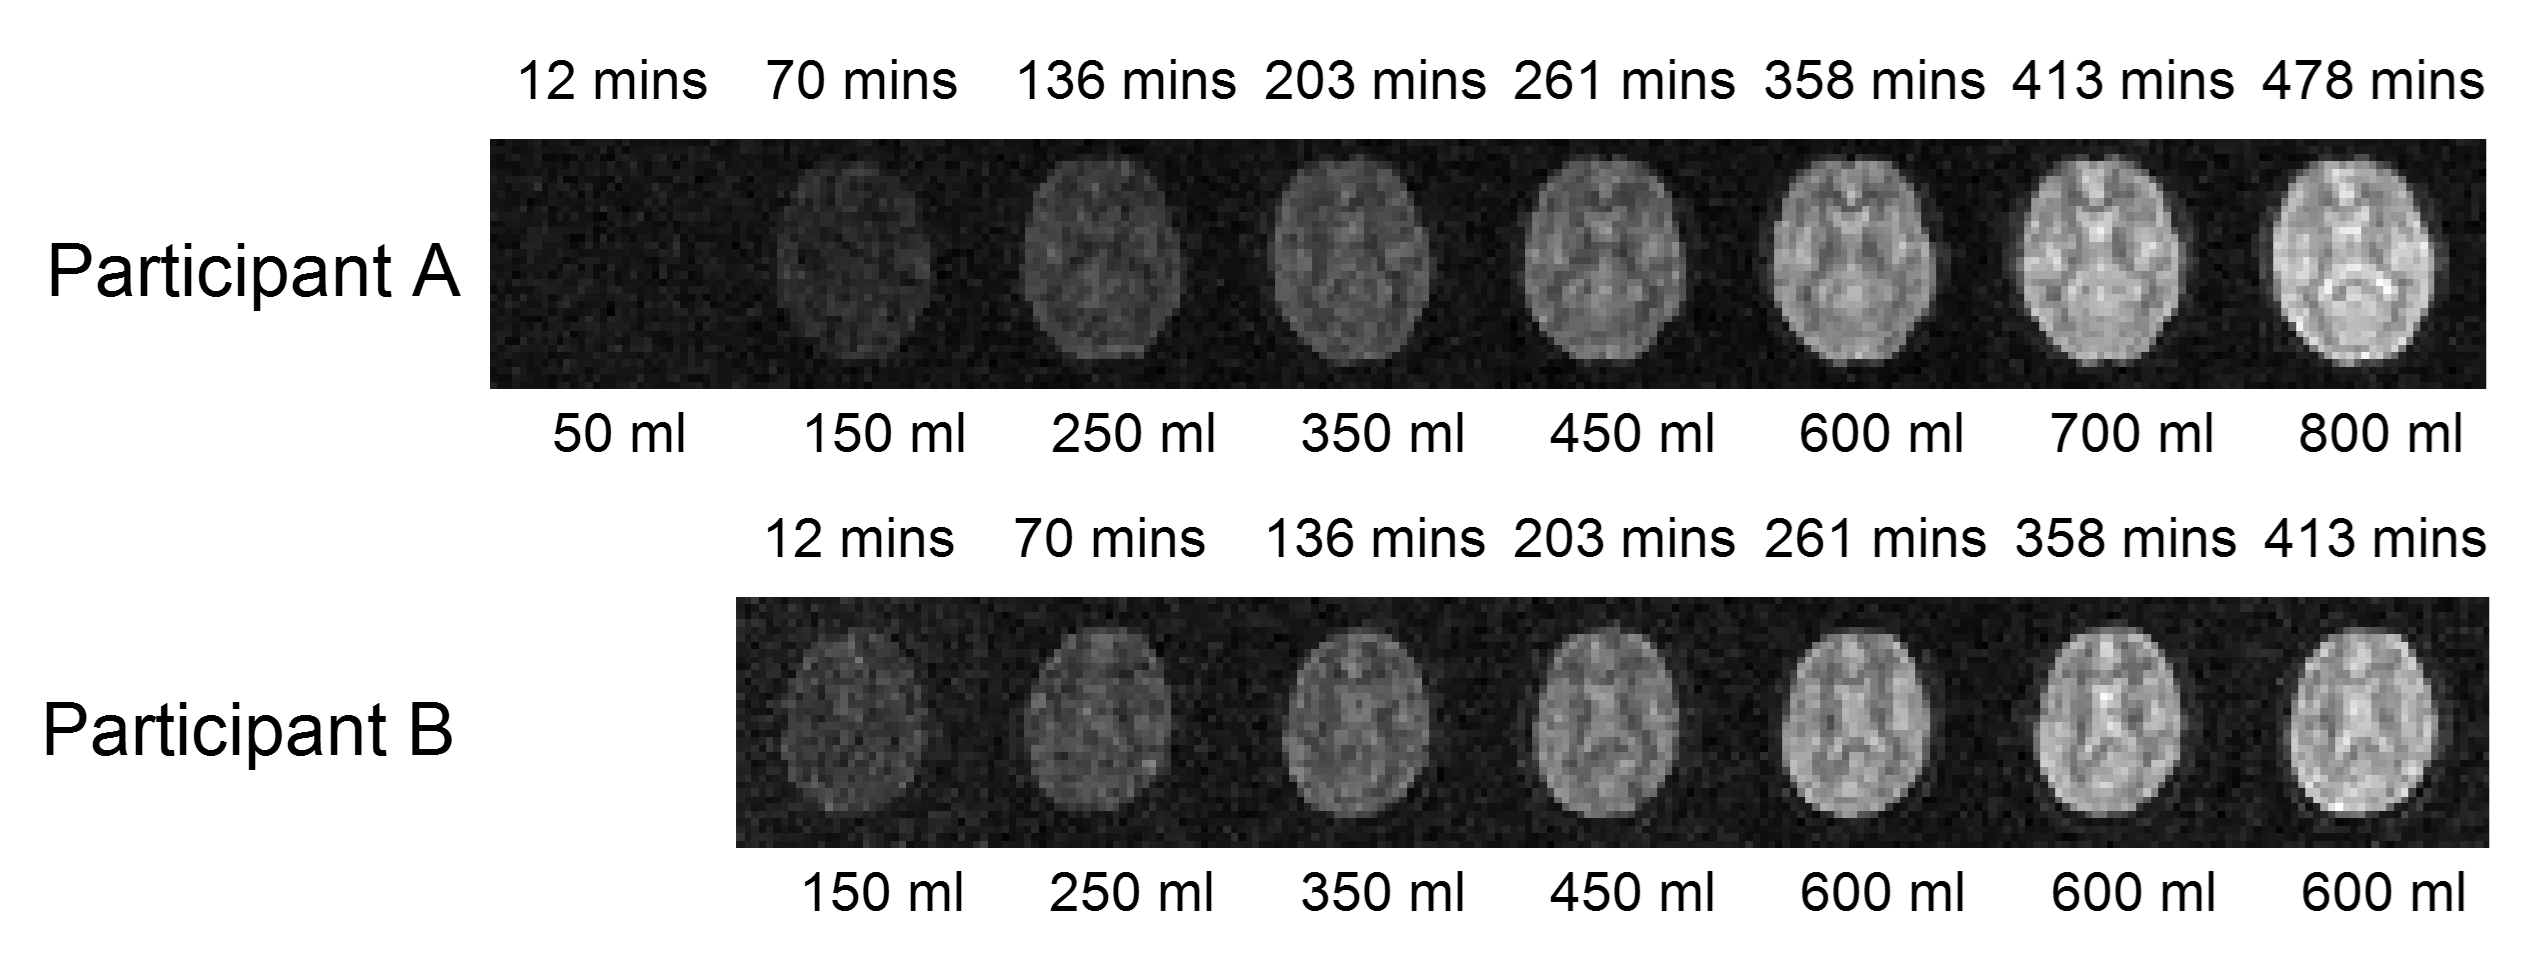
\includegraphics[width=0.9\textwidth]{Figures/D2O/Loading.png}
    \caption{\textit{$^2$H images acquired from two participants at different times during the initial, 8-hr heavy water loading period. The time since the first dose is indicated above each image and the cumulative dose of heavy water is indicated below. A single axial slice spanning the lateral ventricles is shown. The images shown are formed from the average over five echoes (TE$_1$ =8.9 ms, $\Delta$TE=8.4 ms) and have a reduced \ac{FOV} of 204 × 204 mm$^2$.}}
    \label{fig:D2O:Load}
\end{figure}

\subsection{Relaxation Times}

Figure \ref{fig:D2O:R1_R2} shows sagittal and axial relaxation rate maps from two participants, with the dominant feature in the $^2$H maps being the reduced R$_2^*$ and R$_1$ relaxation rates in the ventricles. The elevated R$_2^*$ values seen in deep grey matter structures in the $^1$H maps are not evident in the $^2$H maps. Table \ref{fig:D2O:R_times} reports the average and standard deviation of the $^2$H T$_1$ and T$_2^*$ values, along with $^1$H T$_2^*$ values measured measured in \ac{GM}, \ac{WM} and \ac{CSF} in the four participants. These values were calculated by applying the binarised segmentation masks to the relaxation maps.

\begin{figure}[H]
    \centering
    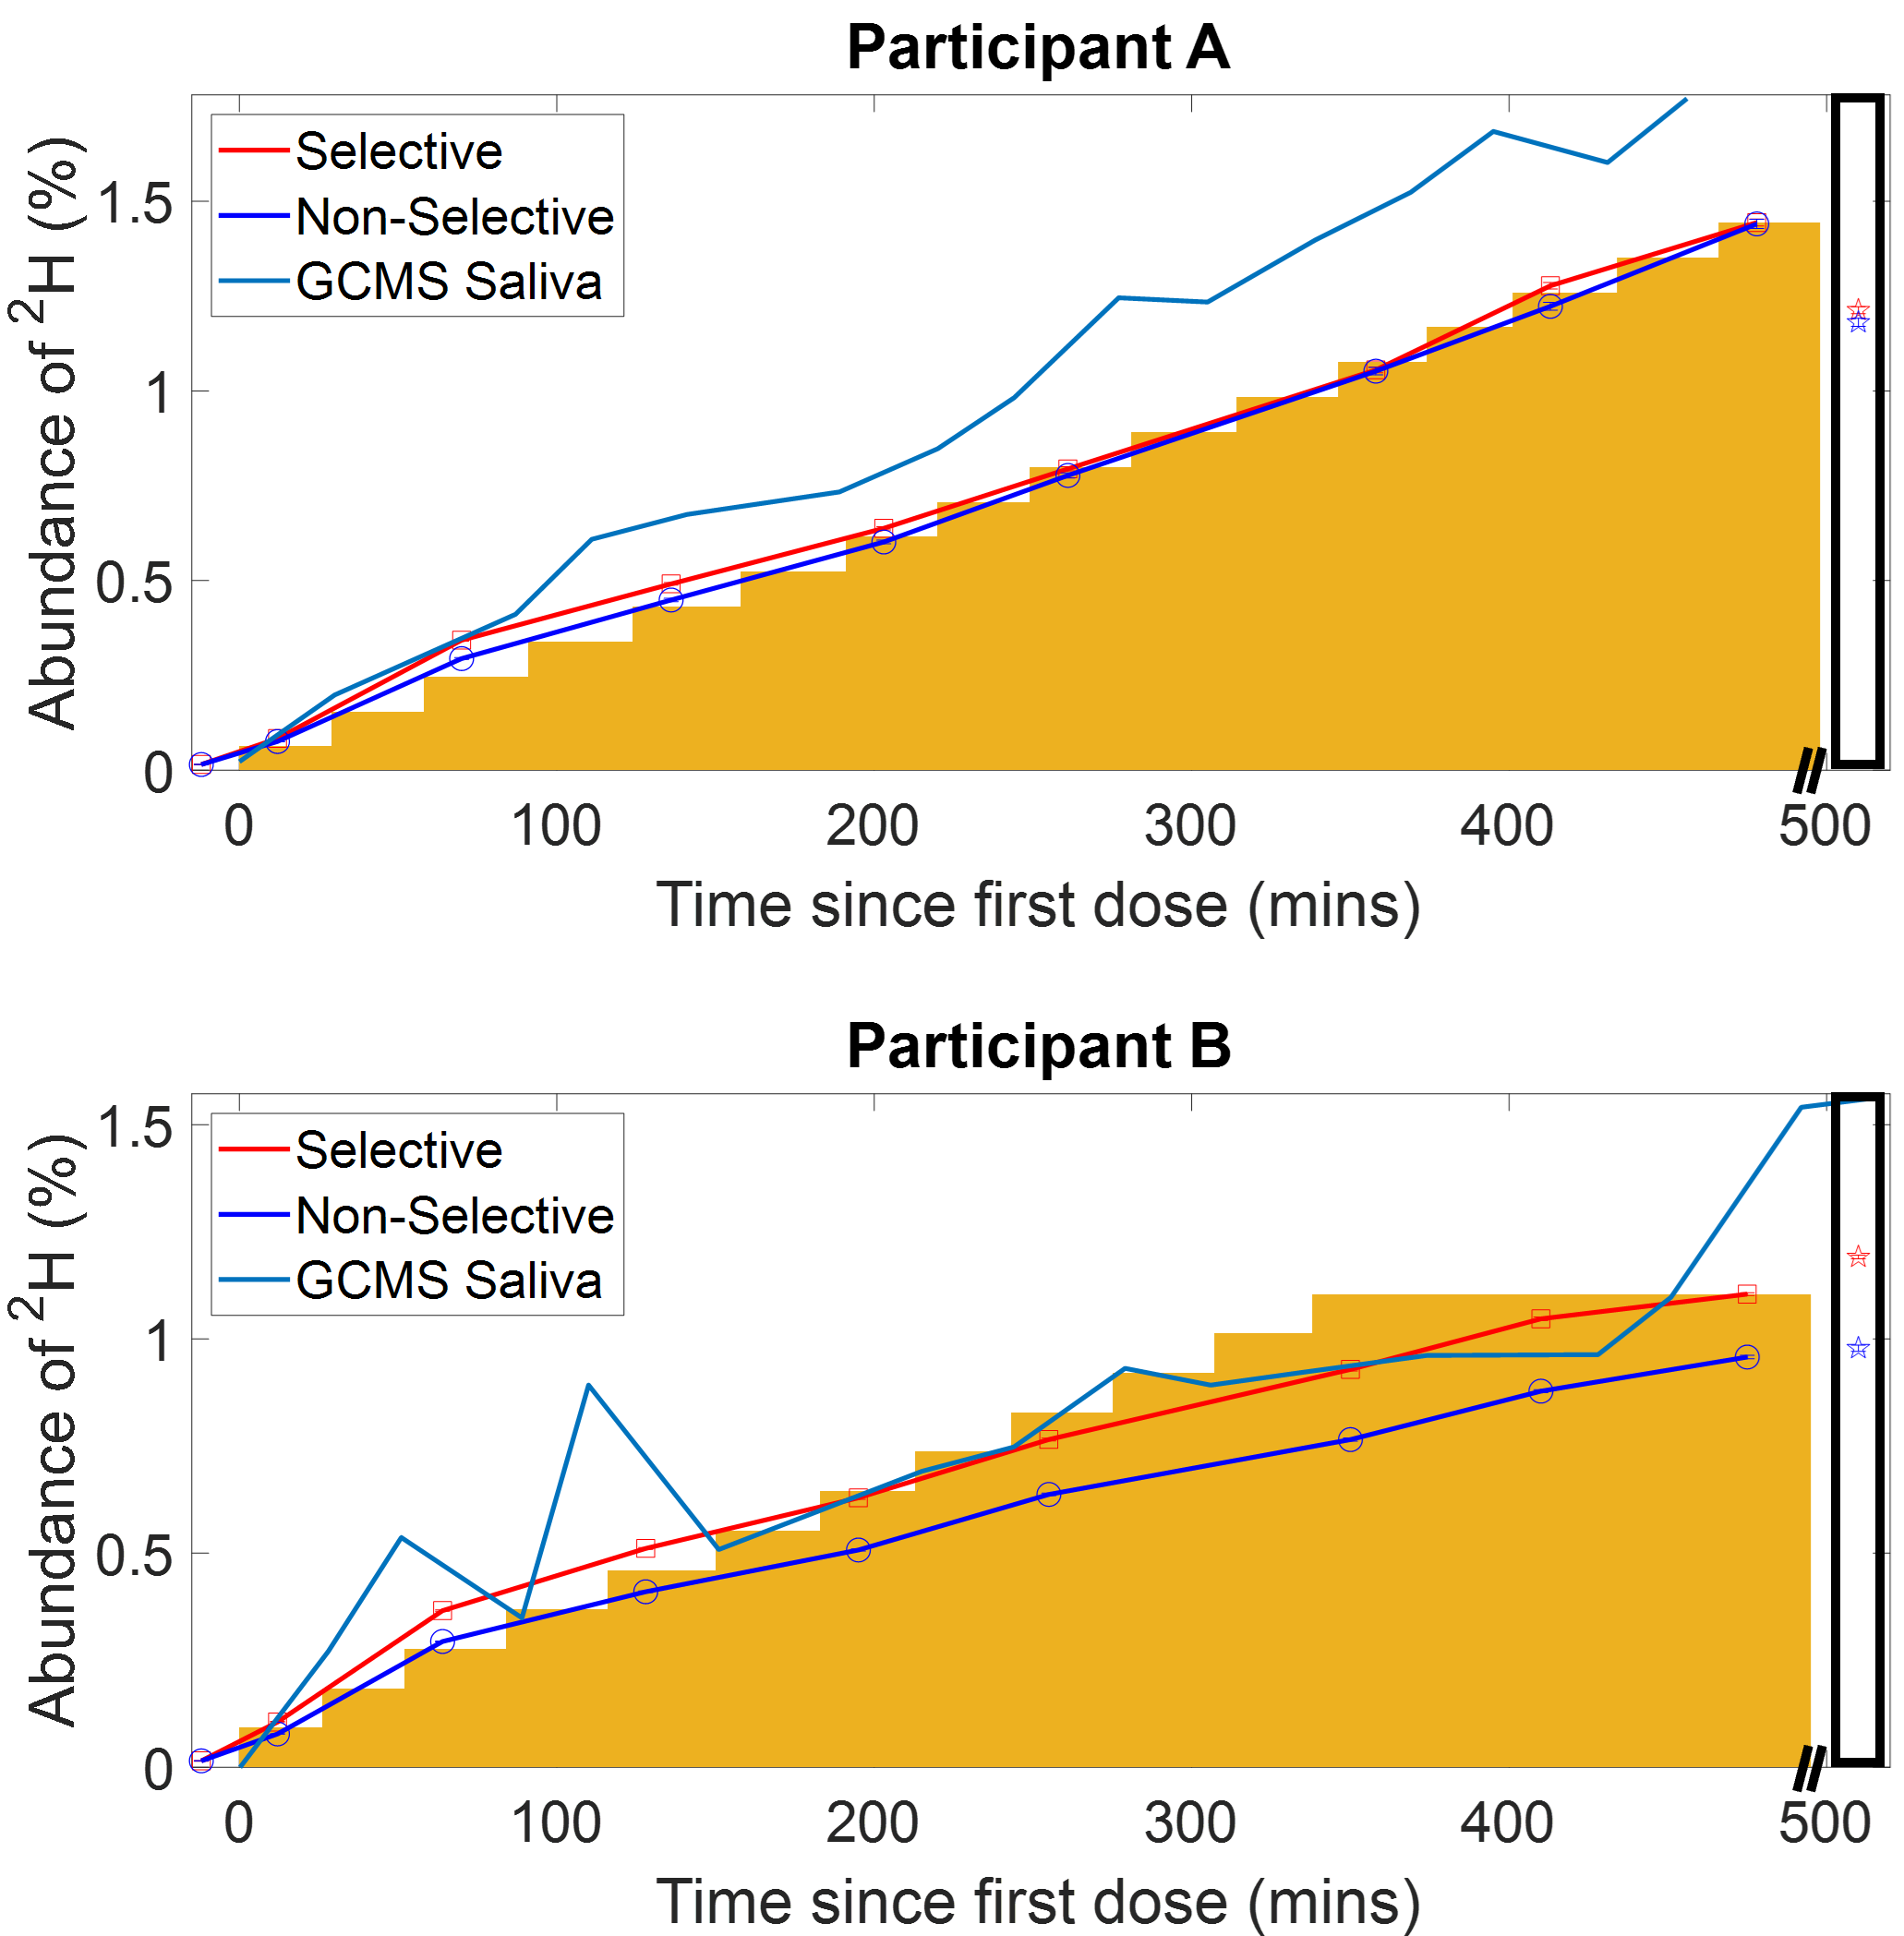
\includegraphics[width=1\textwidth]{Figures/D2O/Bulk_Graph.png}
    \caption{\textit{Time course of the concentration of deuterium in the brain estimated from the $^2$H spectroscopy measurements (red=from 2 cm slice at level of lateral ventricles; blue= whole head). Percentage estimated by scaling by the signal measured at \ac{NA} (assumed to be 0.015\%). The orange blocks indicate the concentration estimated from the cumulative D$_2$O dose and body weight. The measurements made at steady state (after 17 days of loading) are shown in the box at the far right.}}
    \label{fig:D2O:Bulk}
\end{figure}

\begin{figure}[H]
    \centering
    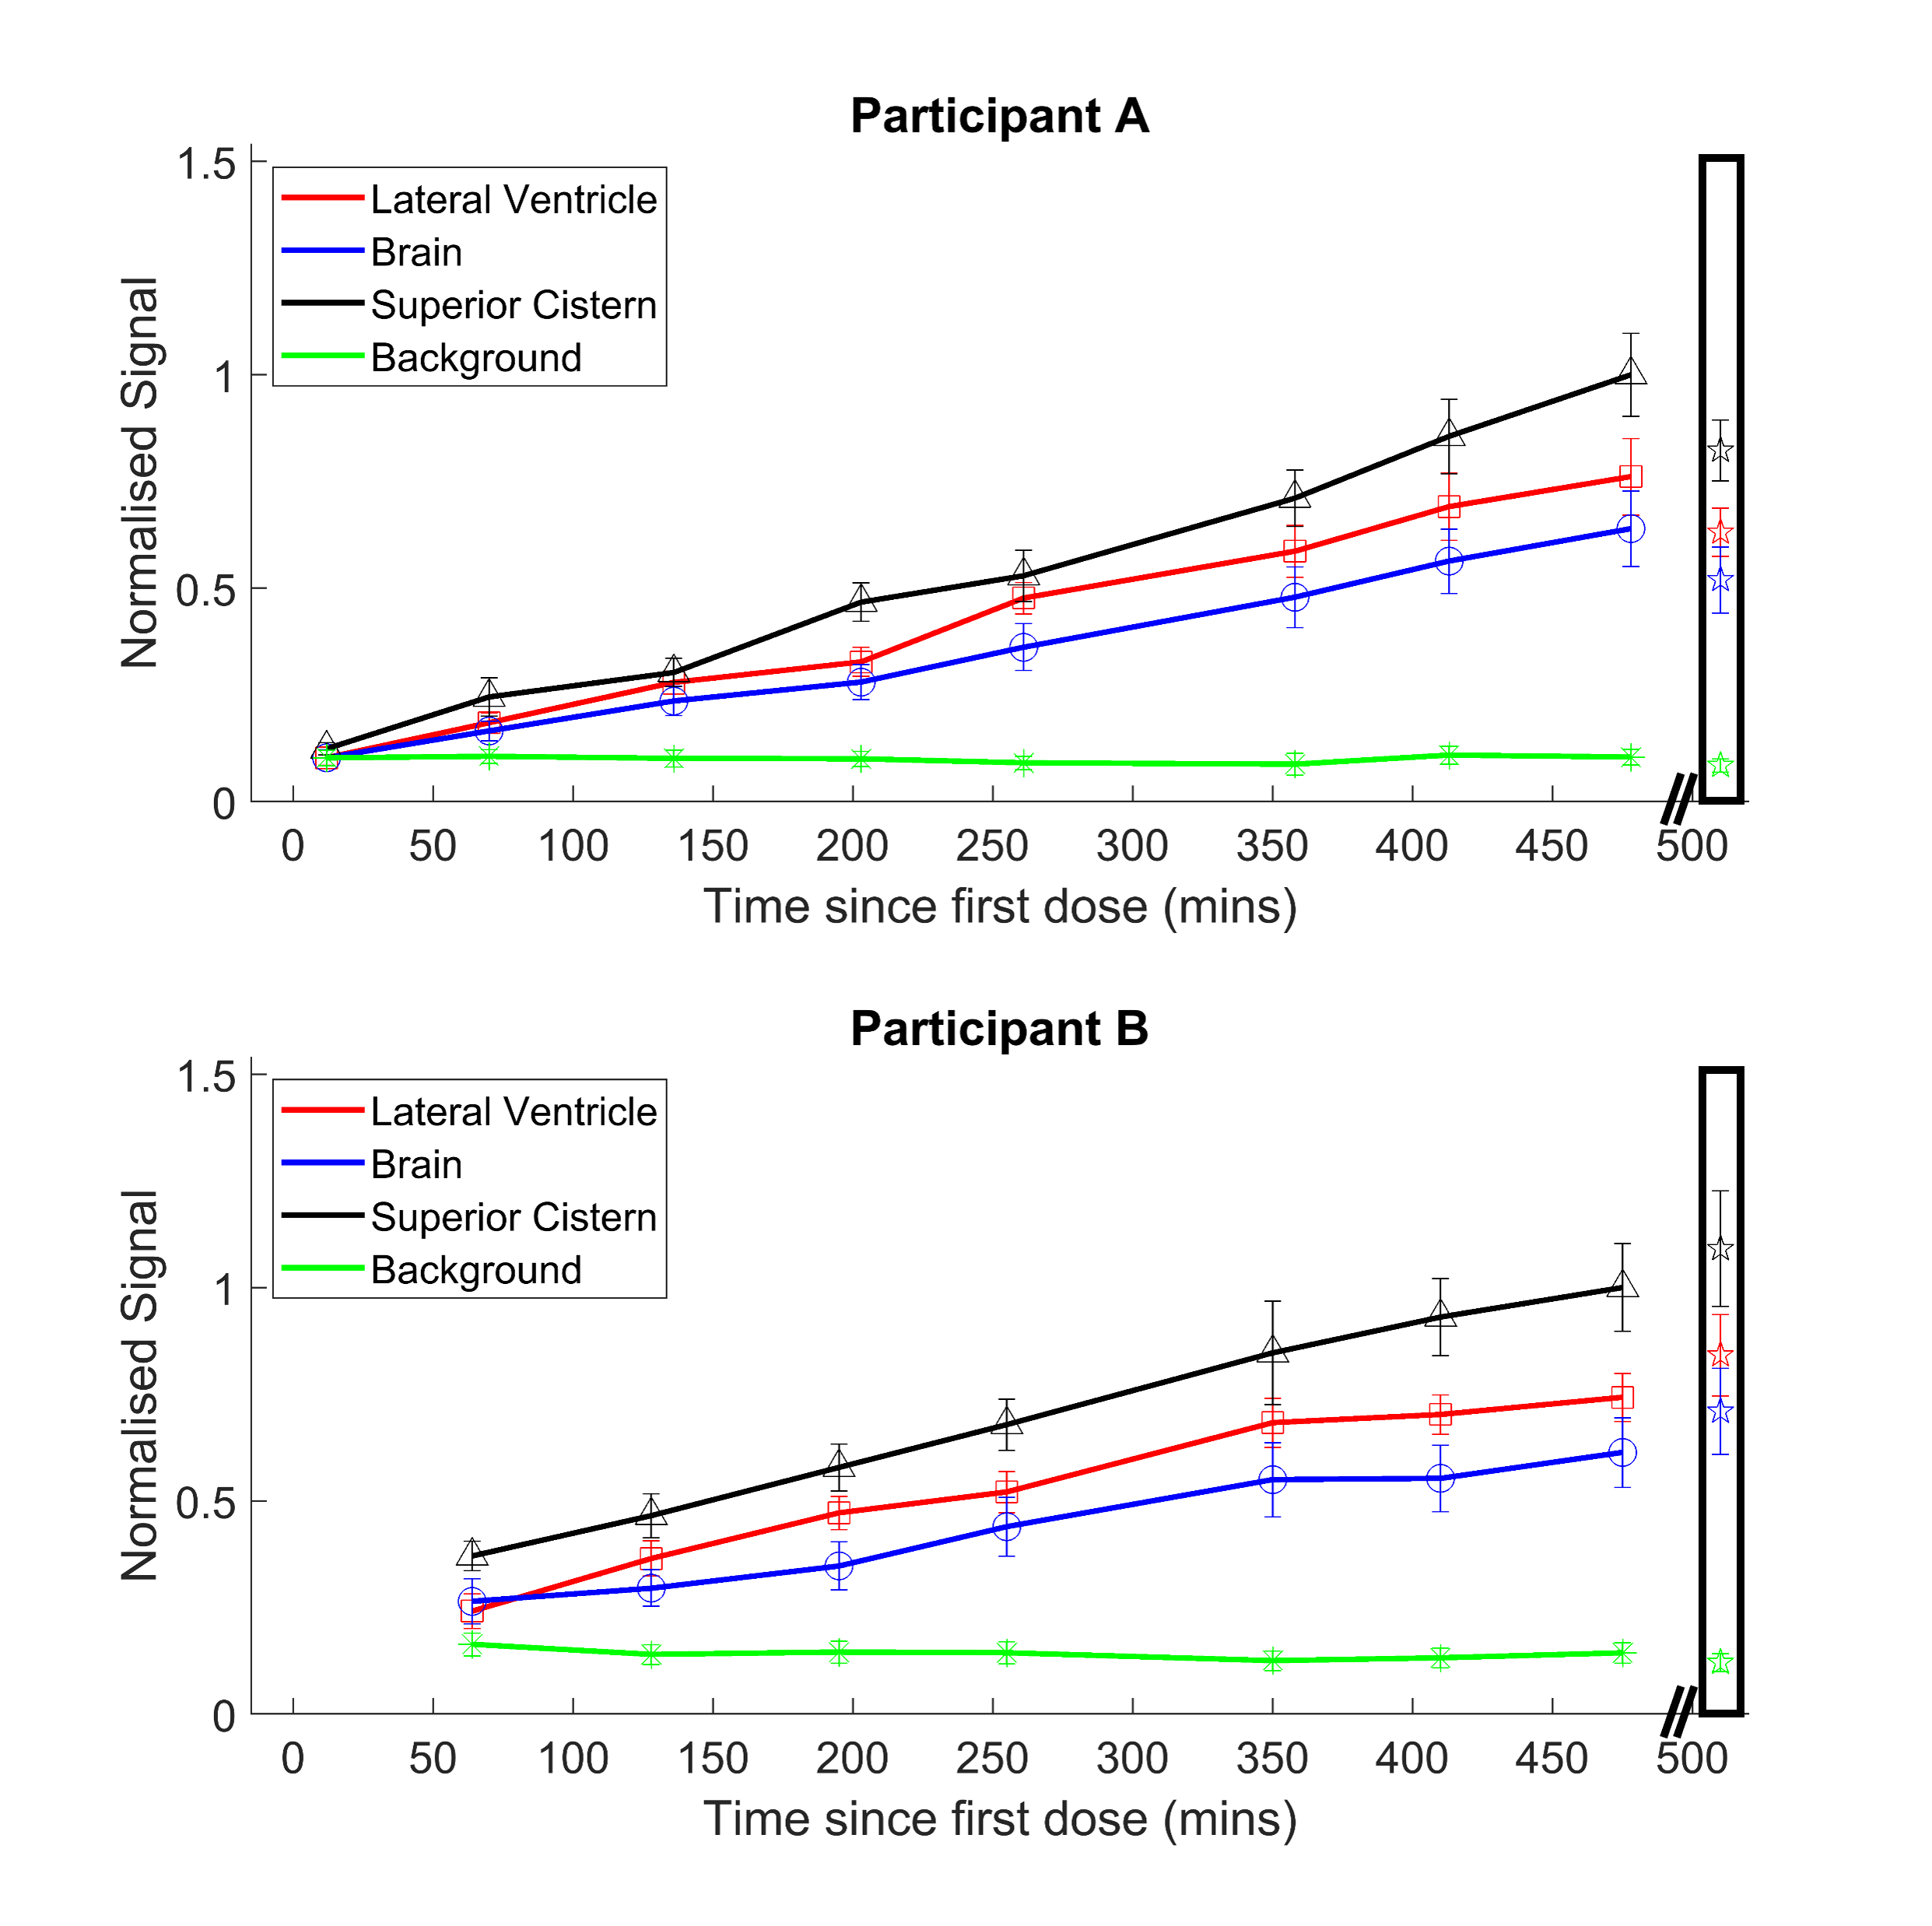
\includegraphics[width=1\textwidth]{Figures/D2O/ROI_Graph.png}
    \caption{\textit{Time course of average signal change in image ROIs (red=lateral ventricle; blue=brain tissue; black=\ac{SC}; green=background noise) in two participants. Signals from all compartments are scaled by the \ac{SC} signal at the final measurement time-point. Scaled signals measured at steady state (after 17-days loading) are shown in the box at the far right.}}
    \label{fig:D2O:ROI_Graph}
\end{figure}

\begin{figure}[H]
    \centering
    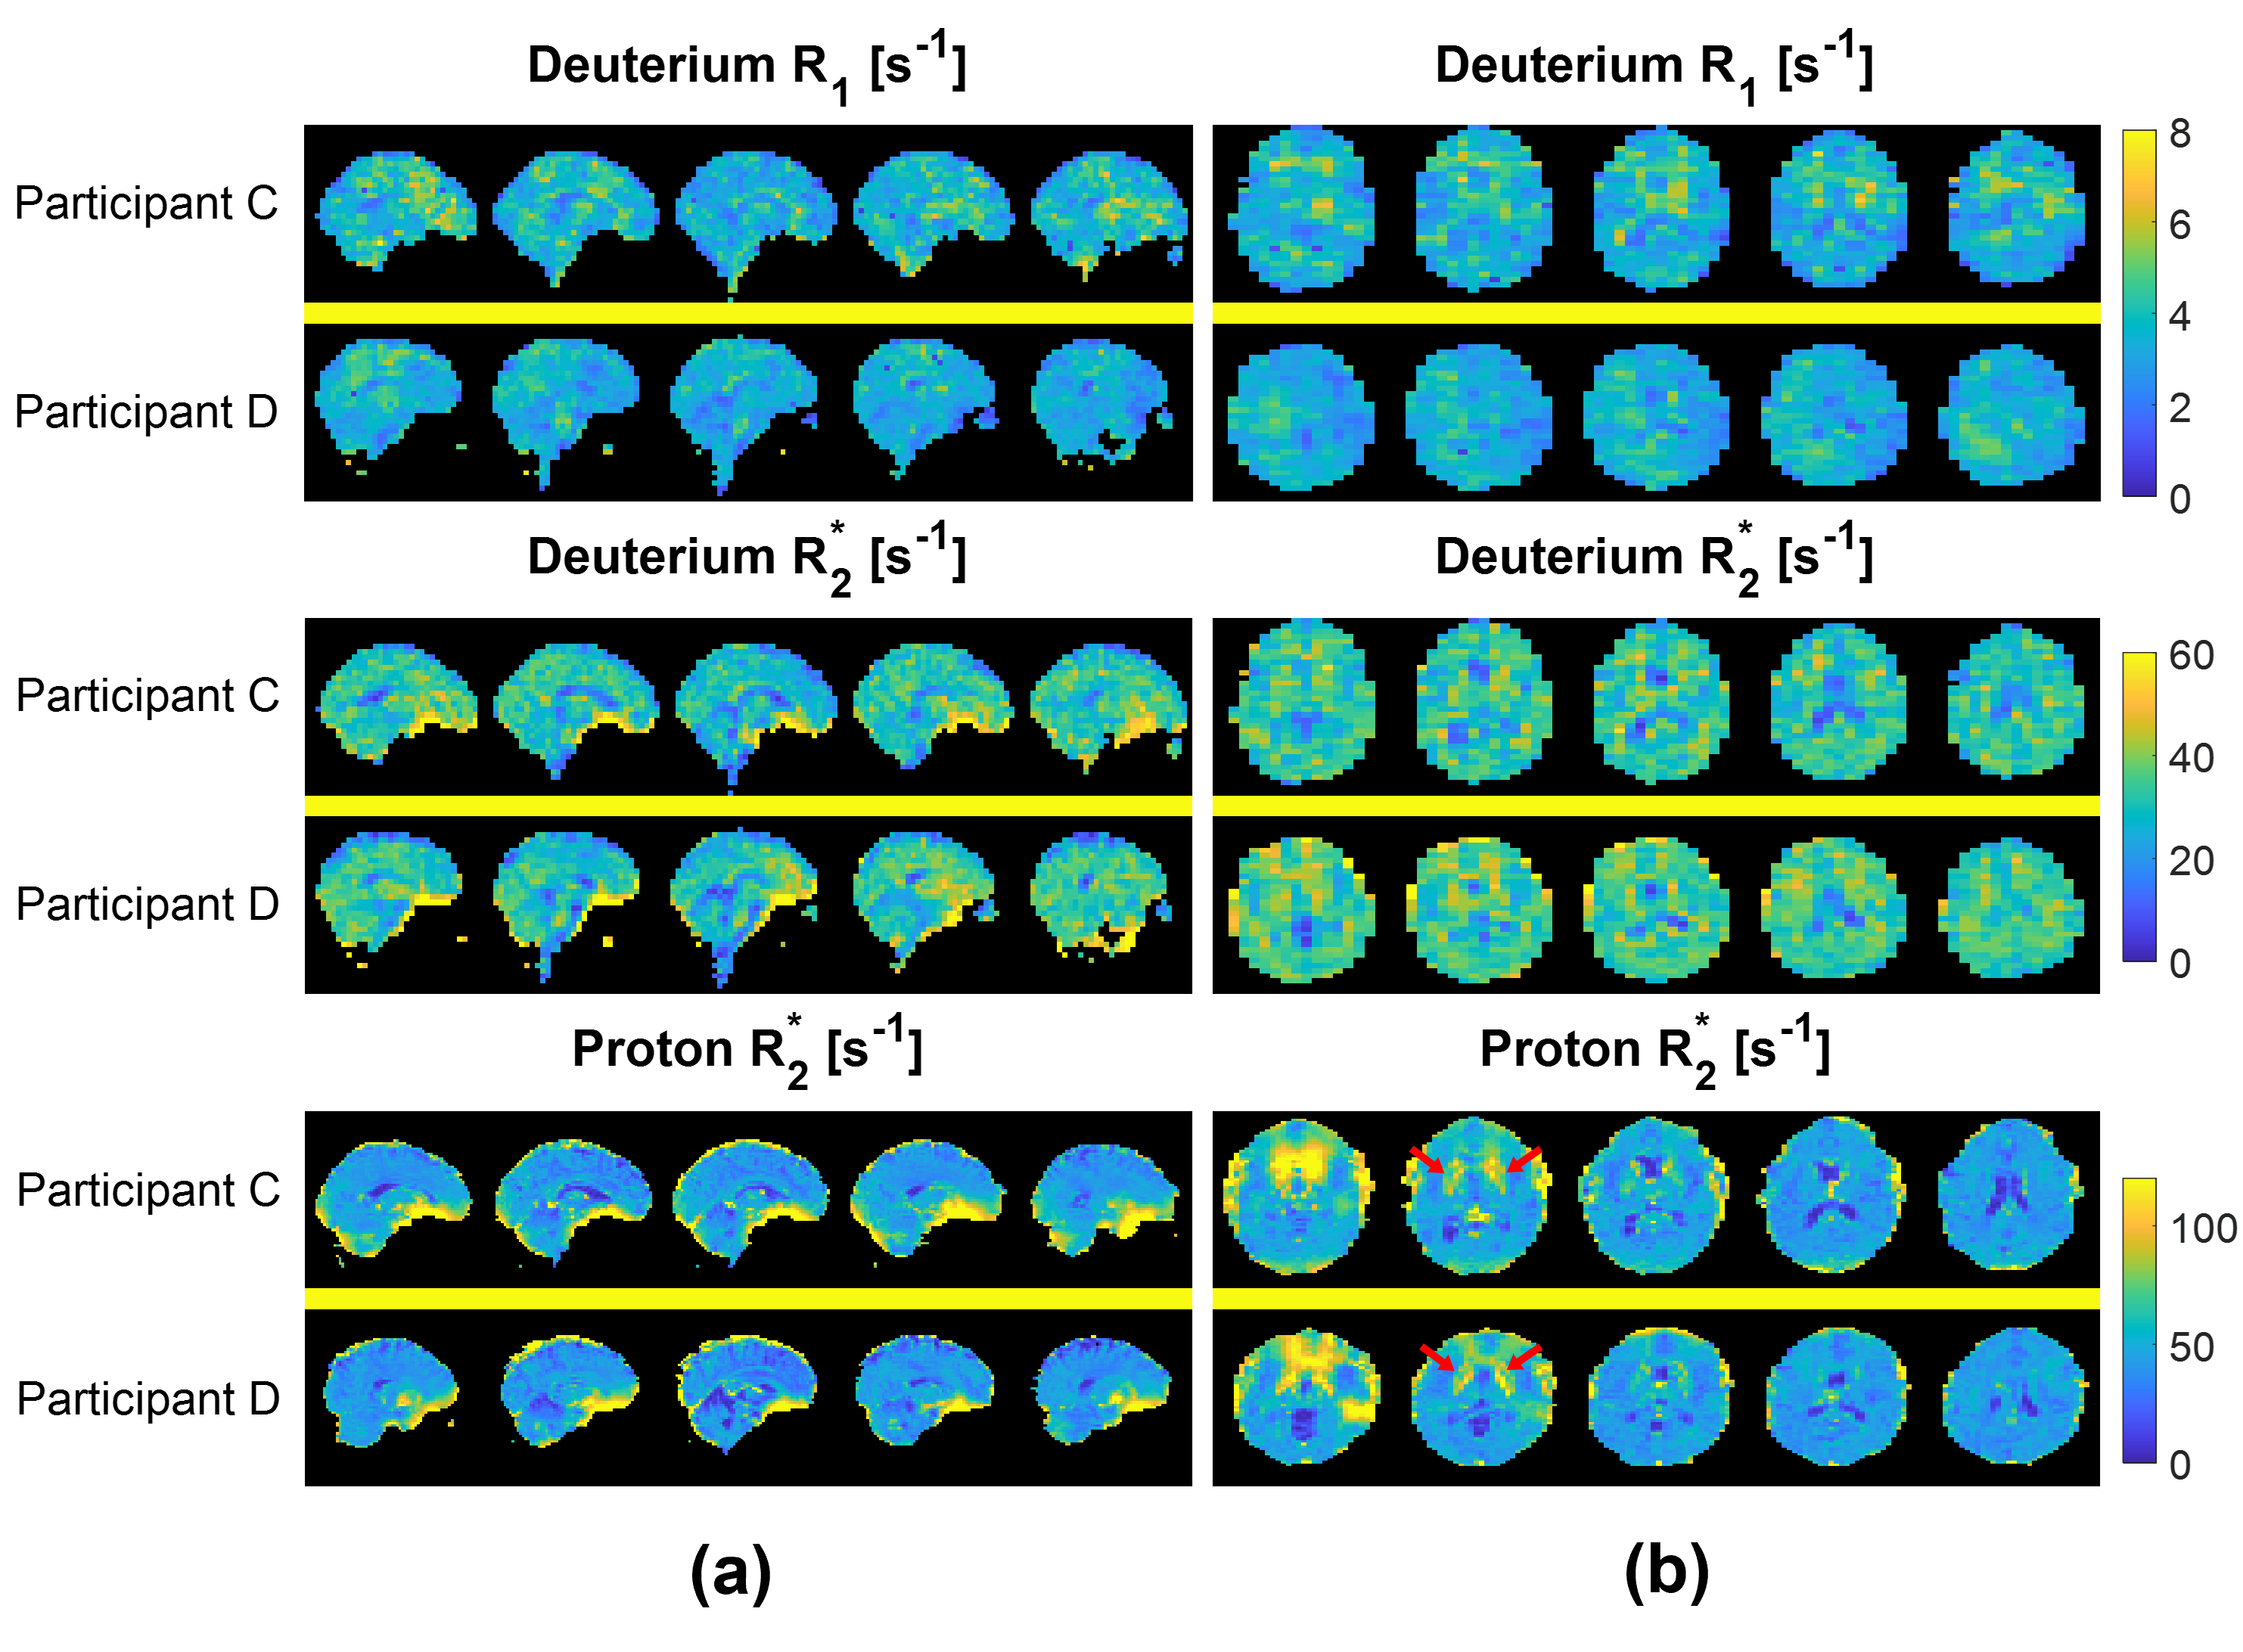
\includegraphics[width=1\textwidth]{Figures/D2O/R1_R2.png}
    \caption{\textit{$^2$H R$_2^*$ and R$_1$ maps are shown along with $^1$H R$_2^*$ maps in sagittal (a) and axial (b) format. Maps show five central slices from Participants C and D. Relaxation maps were calculated from MEGE data equivalent to that displayed in Fig. \ref{fig:D2O:TR_TE}. The elevated R$_2^*$ in iron-rich deep GM structures is evident in the lower slices of the $^1$H maps (red arrows), but is not seen in the $^2$H maps. The images shown have a reduced FOV of 204 × 204 mm$^2$.}}
    \label{fig:D2O:R1_R2}
\end{figure}

% Attempt to create overleaf table, data is too big for fontsize
% \noindent
% \begin{tabular}[H]{ |p{1cm}|p{0.5cm}||p{1cm}|p{1cm}|p{1cm}|p{1cm}|p{1cm}|p{1cm}|p{1cm}|p{1cm}|p{1cm}|  }
%     \hline
%     \multicolumn{2}{|c|}{} & \multicolumn{6}{|c|}{$^2$H relaxation times [ms]} & \multicolumn{3}{|c|}{$^1$H relaxation times [ms]} \\
%     \hline
%     \multicolumn{2}{|c|}{} & \multicolumn{2}{|c|}{CSF} & \multicolumn{2}{|c|}{GM} & \multicolumn{2}{|c|}{WM} & CSF & GM & WM \\
%     \hline
%     Subject & Visit & T$_1$ & T$_2^*$ & T$_1$ & T$_2^*$ & T$_1$ & T$_2^*$ & T$_2^*$ & T$_2^*$ & T$_2^*$ \\
%     \hline
%     A & 1 & 450 $\pm$ 200 & 110 $\pm$ 90 & 280 $\pm$ 100 & 32 $\pm$ 8 & 260 $\pm$ 100 & 30 $\pm$ 10 & 106 $\pm$ 90 & 26 $\pm$ 20 & 27 $\pm$ 20 \\
%     \hline
% \end{tabular}

\begin{table}[H]
    \centering
    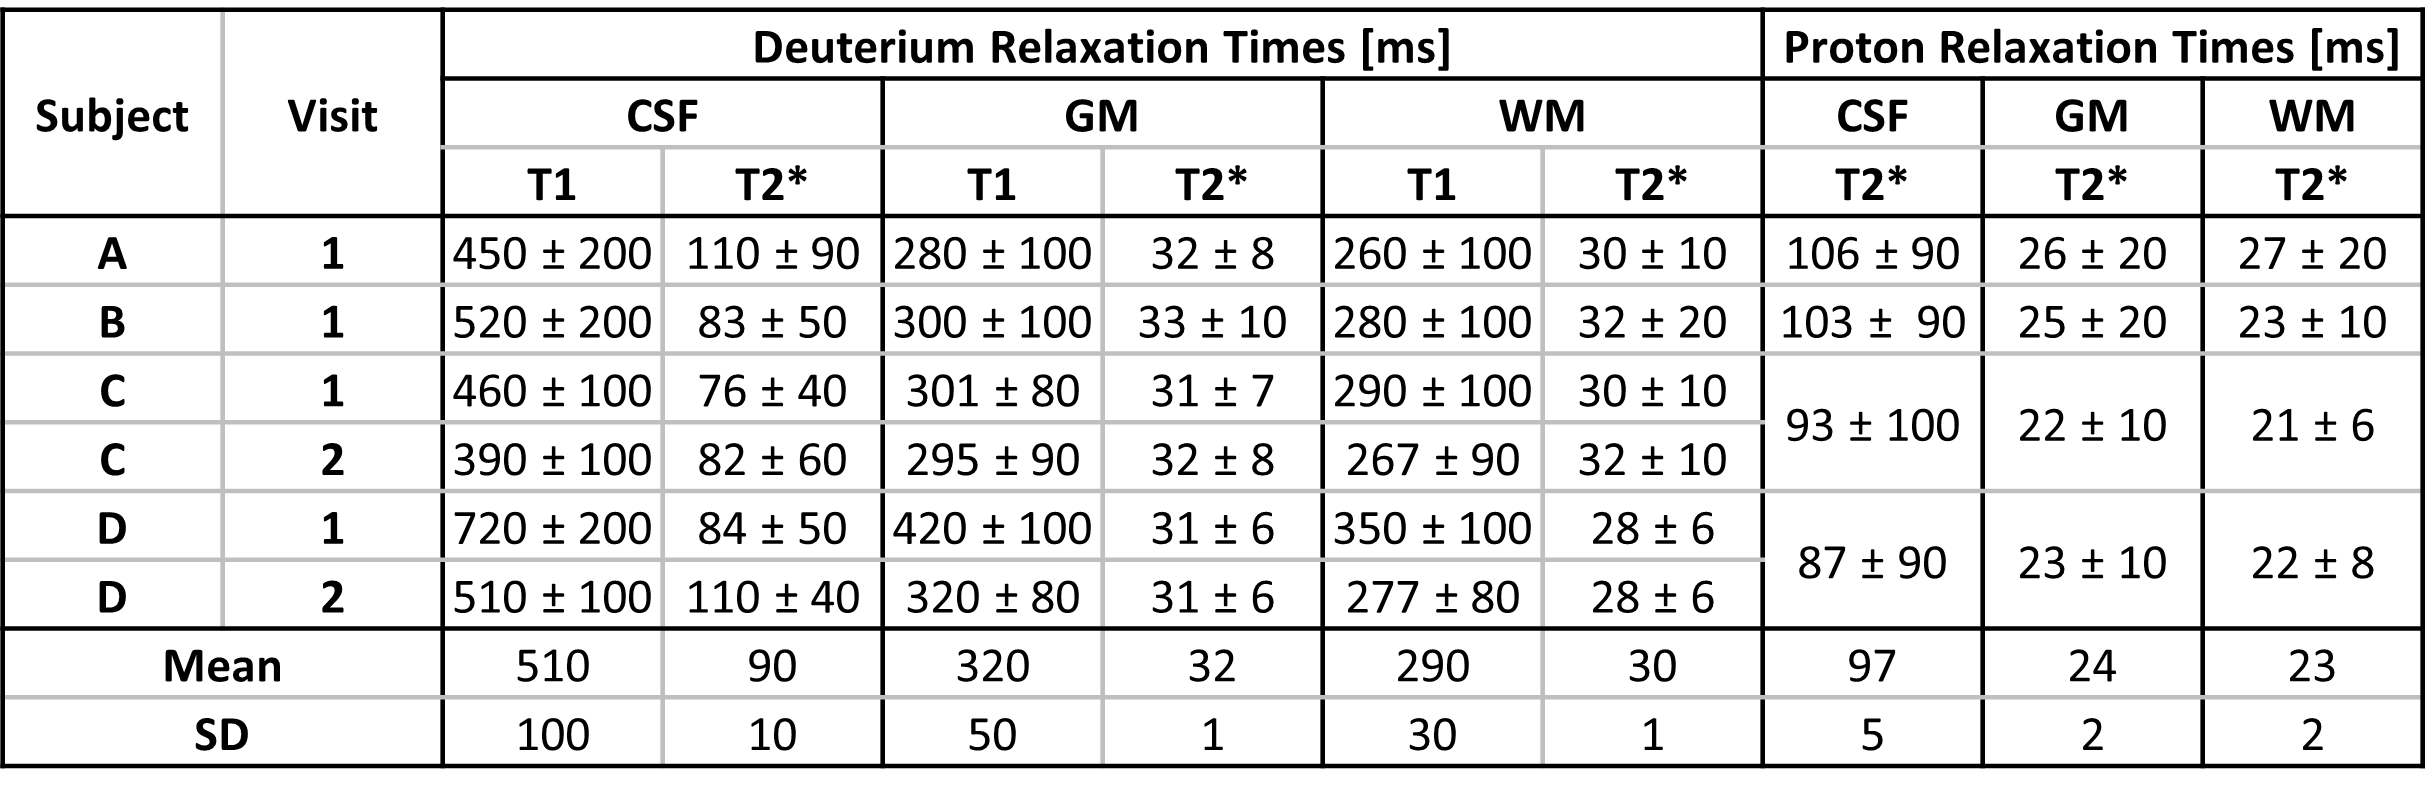
\includegraphics[width=1\textwidth]{Figures/D2O/R_Times.png}
    \caption{\textit{Average and SD of $^2$H (T$_2^*$ and T$_1$) and $^1$H (T$_2^*$) relaxation times in \ac{CSF}, \ac{GM}, and \ac{WM} for different participants and visits. These values were produced by averaging over segmented relaxation time maps, similar to those shown in Fig. \ref{fig:D2O:R1_R2}. Average values and standard deviations across participants are also shown.}}
    \label{fig:D2O:R_times}
\end{table}
 
\section{Discussion}

The results shown in Figs. \ref{fig:D2O:Sag_Full} and \ref{fig:D2O:Load} indicate that $^2$H images of 6 x 6 x 10 mm$^3$ voxel size with a useful \ac{SNR} can be acquired in $\approx$7.5 minutes at 7T with a head-sized bird-cage coil, when participants have been deuterium-enriched to $\approx$1.5\% concentration ($\approx$100 times \ac{NA}). After summing over echo times these images (Fig. \ref{fig:D2O:Load}) showed \ac{SNR} $\approx$16 in brain tissue in the steady-state condition (after 17 days of loading), the contrast in these images is dominated by T$_2^*$-weighting with the \ac{CSF} appearing hyperintense relative to grey and white matter.

The measured relaxation times were reasonably consistent across the six measurements (Table \ref{fig:D2O:R_times}), with \ac{CSF} having significantly higher T$_1$ and T$_2^*$ values than \ac{GM} or \ac{WM} (p $<$ 0.007 for two-sample t-test). The measured T$_1$ and T$_2^*$ values were consistently higher in \ac{GM} than in \ac{WM}, but the differences did not reach statistical significance (T$_1$: p = 0.21; T$_2^*$: p = 0.08). The relatively coarse resolution of the $^2$H images made it difficult to avoid the effects of partial voluming, particularly of \ac{CSF} and \ac{GM}, and the limited range of \ac{TE} and \ac{TR} values reduced the accuracy of measurement of the long T$_1$ and T$_2^*$ values in \ac{CSF}. The average values of the relaxation times are consistent with values reported from non-localised measurements of \ac{HDO} signals in human \cite{DeFeyter2018DeuteriumVivo,DeFeyter2021DeuteriumFuture,Ruhm2021DeuteriumResolution}, cat \cite{Ewy1988DeuteriumSitu} and rat  \cite{DeFeyter2018DeuteriumVivo,Lu2017QuantitativeSpectroscopy} brain.

Focusing on human brain measurements, De Feyter et al. \cite{DeFeyter2018DeuteriumVivo} reported HDO T$_1$ of 346 $\pm$ 5 ms at 4T, while Ruhm et al. \cite{Ruhm2021DeuteriumResolution} measured 362 $\pm$ 6 ms at 9.4T – values which lie between the values for \ac{CSF} (508 ms) and \ac{GM}/\ac{WM} (318/285 ms) measured here at 7T. As expected, the measured $^2$H T$_1$-values are significantly shorter than the corresponding $^1$H values at 7T \cite{Peters2007T27T}, due to the quadrupolar relaxation of $^2$H. The long T$_1$ of \ac{HDO} in \ac{CSF} relative to \ac{GM}/\ac{WM} will lead to greater saturation in the \ac{CSF} signal in short \ac{CSI} measurements used for \ac{DMI} (for example Ruhm et al. used TR = 155 ms \cite{Ruhm2021DeuteriumResolution}) which needs to be considered when quantifying signals from other $^2$H-labelled metabolites using \ac{NA} \ac{HDO} signals. Bi-exponential T$_2$ decay was previously identified at 4T \cite{DeFeyter2018DeuteriumVivo} and 7T \cite{Roig2022Deuterium7T} using non-localised spin echo measurements: at 7T  large (small) pools were found to have relaxation times of 29 $\pm$ 1 (412 $\pm$ 40) ms, respectively \cite{Roig2022Deuterium7T}, consistent with our identification of short and long T$_2^*$ values in \ac{GM}/\ac{WM} (32/30 ms) and \ac{CSF} (90 ms). 

The \ac{TE}-summed \ac{MEGE} images in Figs. \ref{fig:D2O:Sag_Full} and \ref{fig:D2O:Load} show contrast that is dominated by T$_2^*$-weighting, with the \ac{CSF} appearing hyperintense relative to grey and white matter, as is the case in T$_2^*$-weighted $^1$H images. A notable difference between the $^1$H and $^2$H R$_2^*$ maps (Fig. \ref{fig:D2O:R1_R2}) is that deep \ac{GM} structures which appear with elevated R$_2^*$ in $^1$H maps due to their high iron content \cite{Peters2007T27T} do not appear hyperintense in the $^2$H maps. This is a consequence of the dominance of quadrupolar, rather than dipolar, relaxation in the case of $^2$H. The $^1$H R$_2^*$ maps also show larger regions of hyperintensity near the frontal sinuses due to the greater field-inhomogeneity-related intra-voxel dephasing resulting from the higher $\gamma$ of $^1$H. Signals from structures outside the brain (apart from the eyeball) are only evident in the $^2$H images acquired with the shortest \ac{TE} (Fig. \ref{fig:D2O:TR_TE}) most likely because of the very short T$_2^*$ of \ac{HDO} in muscle \cite{Gursan2022ResidualMuscle,Damion2021NaturalT}.

Both the imaging and spectroscopy results shown in Figs. \ref{fig:D2O:Bulk} and \ref{fig:D2O:ROI_Graph} show that changes in \ac{HDO} concentration on the order 0.1\% can be readily monitored and tracked, with spectroscopy data being obtained in one minute. At an estimated concentration of 0.5\% $^2$H, the ratio of signal to background noise varied from $\sim$2.7 (brain) to $\sim$3.1 (\ac{SC}) and these values increased approximately linearly with concentration as expected (Fig. \ref{fig:D2O:ROI_Graph}) to $\sim$steady state levels over the 8-hour loading period. The concentrations estimated from the $^2$H spectra are in reasonably good agreement with the values calculated from the cumulative \ac{D$_2$O} dose and body mass (Fig. \ref{fig:D2O:Bulk}). 

In addition, the signal amplitudes measured from \ac{ROI}s in the brain have similar time-courses maintaining relatively constant ratios, dictated mainly by differences in T$_2^*$-weighting and water fraction in the different brain regions (Fig. \ref{fig:D2O:ROI_Graph}). It is also important to note that as subject C stopped loading (after $\sim$350 minutes) a reduction in the rate of increase in $^2$H concentration is evident in both Figs. \ref{fig:D2O:Bulk} and \ref{fig:D2O:ROI_Graph}, on the scale of minutes. This implies that the $^2$H MR measurements are robust and that the dispersal kinetics of deuterium following oral ingestion of \ac{D$_2$O} are rapid throughout the body on the timescale of the measurements. This is consistent with previous measurements based on blood sampling which indicate that the half-life of absorption into blood is $\approx$12 min, with similar time constants for dispersal into other body water compartments \cite{Davies2001RapidWater,Peronnet2012PharmacokineticHumans}. 

In our experiments the participants came out of the magnet bore between measurements, leading to the potential for changes in signal intensity due to variation of the slice position. Nevertheless the $^2$H signals tracked the monotonically increasing dose and the values measured at maximum dose were similar to those measured 17 days later during the steady state loading period. Although both participants had approximately the same weight and target \ac{D$_2$O} dose, Participant B was only able to ingest 600 ml during the initial loading. The deuterium concentration measured from Participant A was consequently higher at the end of the loading period. The rest of participant B’s loading was completed over the following four days, along with the daily 50 ml top-up and similar concentrations were measured from the two participants in the steady state (Fig. \ref{fig:D2O:Bulk}). The gas chromatography–mass spectrometry measurements of deuterium concentrations in the saliva samples from Participant A and B were 1.51\% $\pm$ 0.09\%, and 1.53\% $\pm$ 0.17\%, respectively. 

Rapid increases in body water enrichment can lead to feelings of dizziness and nausea. These symptoms can occur at relatively low enrichments while equilibrium has not yet been achieved, and are thought to result from temporary effects on the vestibular system due to density changes in the semi-circular canals of the inner ear \cite{Money1974HeavyAlcohol}. The rapid loading was required for the parallel study, but a more gradual increase in heavy water uptake could be used for future MR-loading experiments to minimise these effects. 
%This meant that some of the subjects were unable to finish the rapid loading in the first day. This can be seen in Figs. \ref{fig:D2O:Load}, \ref{fig:D2O:ROI_Graph} and \ref{fig:D2O:Bulk} which is why Participant B was only able to ingest 600 ml out of the 800 ml, despite having approximately the same weight as Participant A, and why the rate of \ac{D$_2$O} loading was slowed. This effect has caused previous participants to withdraw, no female participant was able to complete the initial loading in the first day. There are numerous reasons that could explain this behavior, one of which being possible less body water \% meaning the estimated dosage was too high. This could be explained by reports of women having a higher motion sickness susceptibility \cite{Flanagan2005SexSickness.}, this difference has also been made aware during spaceflight as female crew-members report post-flight vestibular instability symptoms more frequently than men \cite{Reschke2014EffectsSystems}. One possible explanation is the sexual dimorphism in the size of structures in the vestibular system, as many structures have been found to be larger in men \cite{Sato2016Computer-AidedApparatus}. However, no firm explanation on the cause of this apparent motion sickness has been made, it is unknown whether it is affecting this study.  

\section{Conclusion}

$^2$H MR measurements at 7T have been successfully used to track the increase in concentration of $^2$H in brain during \ac{D$_2$O} loading to 100 times \ac{NA}, in four human participants. Gradient echo images with an \ac{SNR} of 16 and a voxel volume of 0.36 ml could be acquired in 7.5 minutes. $^2$H T$_1$ and T$_2^*$ relaxation times from water in \ac{GM}, \ac{WM} and \ac{CSF} have also been measured at 7T. These relaxation times can be applied in research protocols using the \ac{NA} $^2$H signal from water for calibration and concentration calculations. This lays the ground work for further studies involving ingested \ac{D$_2$O} in order to measure lipid turnover in Chapter \ref{Chap:Lipid}.In future work we aim to track uptake from a single \ac{D$_2$O} dose on a shorter time scale, using faster, interleaved acquisition of $^2$H images and spectra. 

A $^2$H \ac{EPI} acquisition has been used to demonstrate the possibility faster scanning, in 48 minutes of scanning 75 3D image dynamics were acquired ($\sim$38 s each). A healthy human participant was scanned at 7T with a \ac{FOV}: 288 x 288 x 240 mm$^3$, voxel size: 6 x 6 x 10mm$^3$, \ac{TR}: 250 ms, TE: 13.8 ms, flip angle:70$^\circ$, 75 dynamics, \ac{EPI} factor: 23. The participant was taking part in the studies in Chapter \ref{Chap:Lipid} and \ref{Chap:Quad} at the time of scanning and therefore followed the loading regime outlined there. The participant had completed the initial loading and was in the steady-state period. Immediately prior to scanning their 50 ml daily topup was ingested, which can be seen in the first few dynamics of Fig. \ref{fig:D2O:EPI}. The data was de-noised using a Tucker decomposition with a core matrix size of 24 x 24 x 12, afterwards the slices shown were averaged over the centre five sagittal slices. Each individual slice is shown after averaging all the temporal dynamics in Fig. \ref{fig:D2O:EPI_avg}, here no de-noising is applied.

\begin{figure}[H]
    \centering
    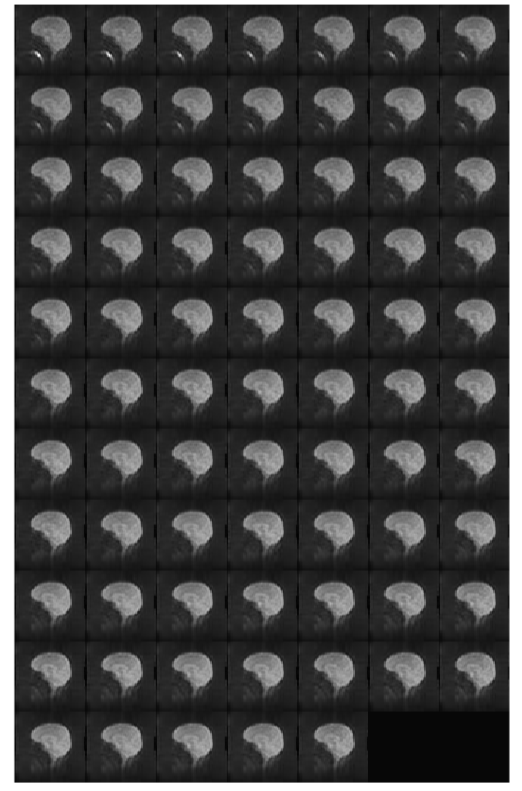
\includegraphics[width=1\textwidth]{Figures/D2O/EPI.png}
    \caption{\textit{Time-course from the five centre averaged sagittal slices of a healthy human brain in vivo, during the steady-state of D$_2$O loading, acquired using an \ac{EPI} acquisition with 75 dynamics, tuned to the $^2$H resonance at 7T.}}
    \label{fig:D2O:EPI}
\end{figure}

\begin{figure}[H]
    \centering
    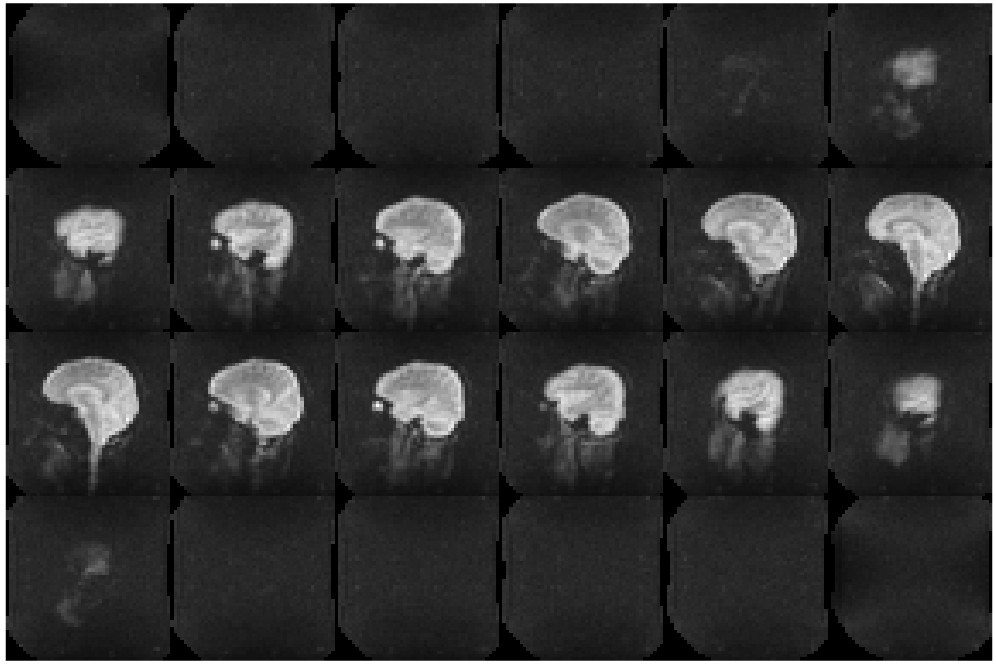
\includegraphics[width=1\textwidth]{Figures/D2O/EPI_avg.png}
    \caption{\textit{Individual sagittal slices of a healthy human brain in vivo, during the steady-state of D$_2$O loading, using an \ac{EPI} acquisition averaged over all 75 dynamics, tuned to the $^2$H resonance at 7T.}}
    \label{fig:D2O:EPI_avg}
\end{figure}

\newpage
\chapter{Comparing D$_2$-glucose and D$_7$-glucose in DMI}
\label{Chap:Glucose}

\section{Introduction}

\ac{DMI} is a \ac{MRSI} method that enables substrates and metabolic products that are labelled with the non-radioactive hydrogen isotope $^2$H, to be mapped \textit{in vivo}. The scientific impact of $^2$H and usage in the real world has increased greatly since its existence was first theorised \cite{Urey1932AConcentration}, and it was not long before its potential for biological applications was recognised \cite{Schoenheimer1935DeuteriumMetabolism, Schoenheimer1938TheMetabolism}. Of particular interest is the use of glucose as the administered labelled precursor molecule, as this can provide a direct probe of glucose metabolism. Whilst the most common current uses for $^2$H for \textit{in vivo} \ac{NMR} measurements involve deuterated glucose, initially it was \ac{D$_2$O} that was ingested to elevate $^2$H levels for use in \ac{NMR} \cite{Brereton1986PreliminarySpectroscopy, Irving1987InSpectroscopy}, particularly to investigate lipid metabolism. The most useful forms of deuterated glucose are those whose carbon-bonded hydrogen atoms in the first and sixth positions have been replaced by deuterium because these substitutions are the only ones that are transferred to pyruvate, and then to either lactate (Lac) or to a combination of glutamate and glutamine (Glx) via the \ac{TCA} cycle in the mitochondria. For this reason, [6,6'-$^2$H$_2$] glucose has been a common choice of labelling (isotopologue), providing twice the number of $^2$H labels as would [1-$^2$H] glucose, and this form of labelled glucose has been used in many \textit{in vivo} studies ranging from preclinical work \cite{Lu2017QuantitativeSpectroscopy, Meerwaldt2023InImaging} to demonstration in humans  \cite{DeFeyter2018DeuteriumVivo, Roig2022Deuterium7T}. Lactate and Glx as well as non-metabolised glucose and water (\ac{NA} plus an additional amount caused by label-loss during various processes) become detectable via either choice of labelling. The detected lactate and Glx provide information about the tissue’s propensity to metabolise glucose via glycolysis or the oxidative phosphorylation pathway, and thereby an important clinical potential of DMI is identified, since many tumour cells exhibit an increased tendency for glycolysis. This manifests in higher than usual lactate production;  the well-known Warburg effect \cite{Warburg1956OnCells}.    

$^2$H \ac{NMR} measurements following labelled glucose ingestion or injection allow information on downstream metabolite concentrations to be quantified to obtain metabolic flux measurements, without the use of ionising radiation. In contrast \ac{PET} scans using \ac{FDG} involve ionising radiation and only provide information on glucose uptake. Besides the effect of cancer and other disease states, brain metabolism is also altered locally, albeit temporarily, as part of normal function. This might occur when a part of the brain is activated by a task or stimulus, such as by visual stimulation. For example it has been previously shown many times that there is metabolic activation in the visual cortex following visual stimulation \cite{Kushner1988CerebralStimulation, Beland-Millar2018FluctuationsStimulation}. Lactate increases \cite{Prichard1991LactateStimulation., Sappey-Marinier1992EffectSpectroscopy, Fernandes2020MeasurementT}, and glucose decreases \cite{Lin2012InvestigatingT} in the visual cortex following visual stimulation have been measured using $^1$H \ac{MRS}. $^{13}$C \cite{Chhina2001MeasurementSpectroscopy} \ac{MRS} has been used to measure \ac{TCA}-related changes during activation in the visuall cortex, and $^{31}$P \ac{MRS} has been used to measure signal changes in lactate, phosphocreatine and inorganic phosphate in the visual cortex during stimulation\cite{Sappey-Marinier1992EffectSpectroscopy}. Glucose signals are not present in these measurments. It is important to note that significant increases in glutamate (2\%) and decreases in glutamine (8\%) have also been shown during activation \cite{Lin2012InvestigatingT}.
 
In its simplest form, \ac{DMI} is relatively straightforward to implement using a pulse-acquire \ac{CSI} sequence, usually without the need for water suppression because of the low concentration of naturally occurring deuterated water. In most cases, \ac{DMI} spectra are also simpler to analyse than proton spectra. If using glucose as the labelled substrate, there are just four metabolites to consider: water (\ac{HDO}), glucose, Glx, and lactate. This relative simplicity can be regarded as a positive attribute in the context of potential clinical translation. However, the generally low \ac{SNR} of \ac{DMI} is not a favourable characteristic, and means that data is often acquired with low spatial resolution, often with voxels of around 8 ml \cite{DeFeyter2021DeuteriumFuture, deGraaf2020OnImaging} in volume; the smallest reported voxel size to date in humans is 2.97 ml \cite{Ruhm2022Dynamic9.4T}, in measurements made at a high magnetic field strength of 9.4 T. Low \ac{SNR} and spatial resolution can potentially be improved upon by performing \ac{DMI} scans based upon indirect detection using $^1$H \ac{MRSI} \cite{vanZijl2020SpectroscopicFluxes, Bednarik2021DeuteriumBrain, Niess2023Reproducibility3T, Ruhm2022Dynamic9.4T}. This has the benefit of not requiring deuterium-specific hardware, but this comes at the expense of often requiring a more complex acquisition scheme and post-processing analysis. Another method of increasing \ac{SNR} in \ac{DMI} is to implement de-noising during post-processing analysis. This has been shown to improve \ac{SNR} in \ac{MRSI} using low rank approximations \cite{Nguyen2013DenoisingApproximations}. Similar techniques using Tucker decomposition \cite{Tucker1966SomeAnalysis, Bader2007EfficientTensors} have been applied to \ac{DMI} data with notable \ac{SNR} improvements \cite{vonMorze2021ComparisonT, Kreis2020MeasuringMRI}.

\begin{figure}
    \centering
    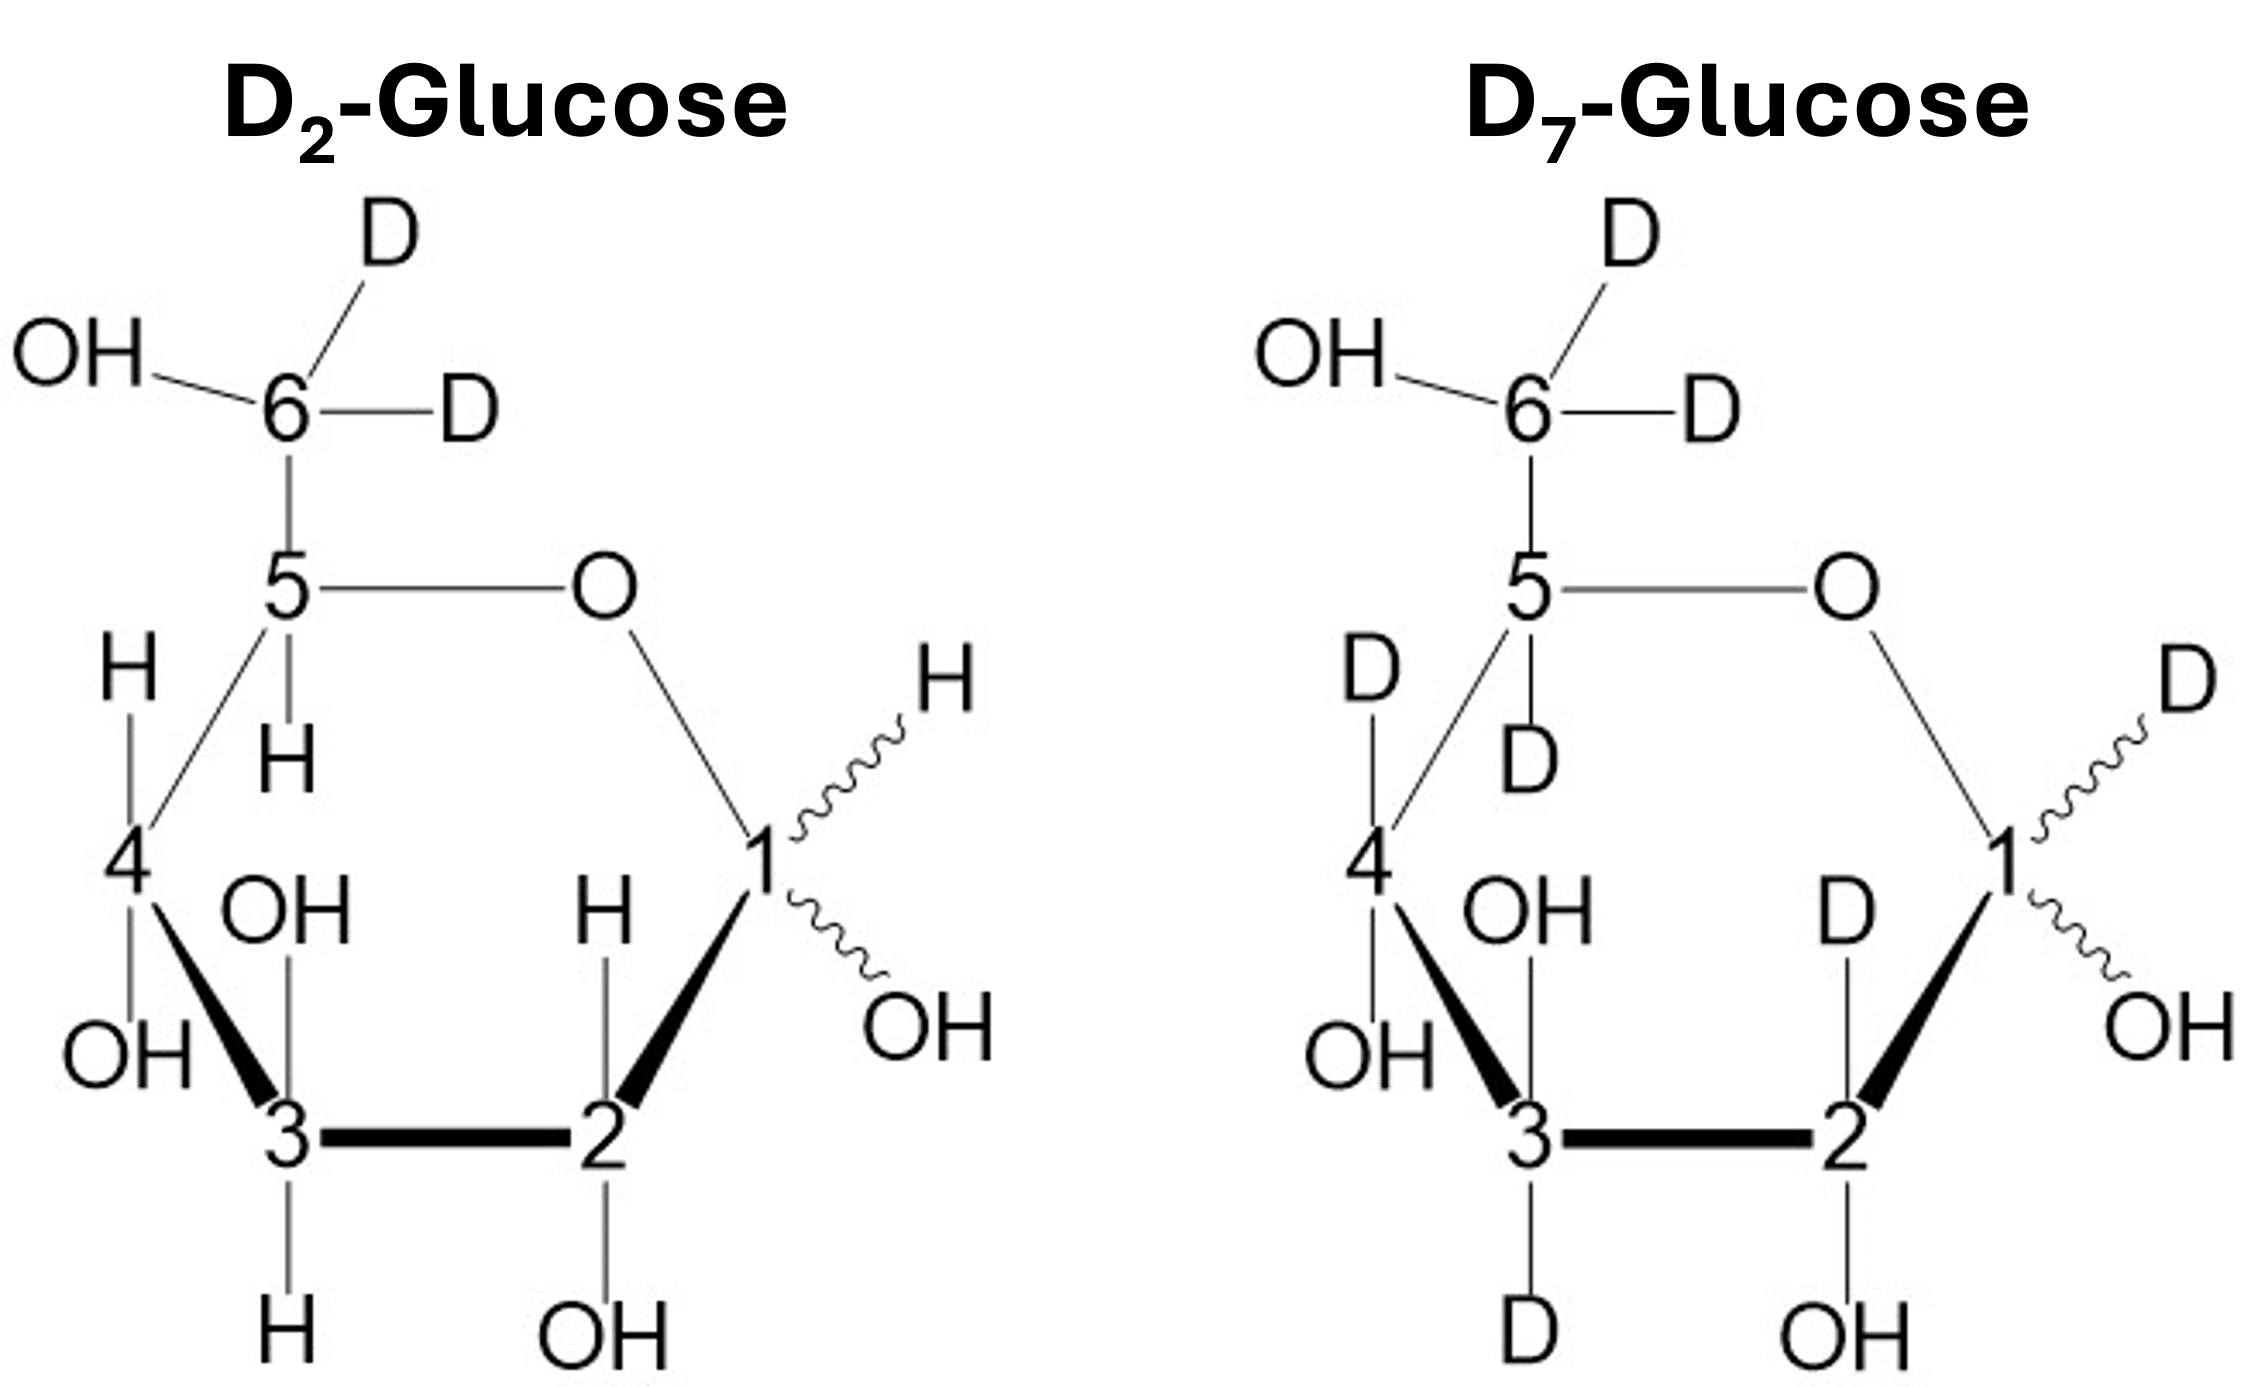
\includegraphics[width = 1\textwidth]{Figures/Glucose/Glucose.png}
    \caption{\textit{The chemical structure of D$_2$ (left) and D$_7$-glucose, where D indicates deuterium atoms and each number refers to a different carbon atom position.}}
    \label{fig:Glu:Glucose}
\end{figure}

Other labelled compounds than D$_2$-glucose have also been used to investigate \textit{in vivo} metabolism in conjunction with \ac{DMI} in animal experiments. For example [6,6'-$^2$H$_2$] fructose has been used to investigate liver cancer \cite{Zhang202366-2H2Cancer}. Fructose was found to have a similar spectral appearance as the glucose, with slightly different kinetics. Intravenous injection of deuterated acetate ([$^2$H$_3$] acetate) has been used to investigate myocardial metabolism \cite{Wang2021NoninvasiveImaging} and tumour metabolism \cite{DeFeyter2018DeuteriumVivo}, where acetate accumulation and Glx changes were tracked.

One important way of increasing the $^2$H signal is to use a form of deuterated glucose with a larger number of $^2$H labels. Since there are twelve hydrogen atoms in the glucose molecule, all twelve could potentially be substituted with $^2$H atoms. However, atoms in the hydroxyl groups exchange rapidly with the surrounding water and therefore are not usually useful in metabolic applications. The seven other locations in which the $^2$H atoms are directly carbon-bonded are less labile and potentially useful labelling sites, yielding the form [1,2,3,4,5,6,6'-$^2$H$_7$]-glucose (D$_7$-glucose). Compared with [6,6'-$^2$H$_2$]-glucose (D$_2$-glucose), the $^2$H spectrum of D$_7$-glucose should contain a factor of 7/2 times more components, many of which overlap due to the broad linewidths of $^2$H, thus producing a gain in \ac{SNR}. The $^2$H atoms in the C1 and C6 positions (in the absence of label-loss) will be transferred to lactate or Glx molecules \cite{DeFeyter2020DeuteriumBrain}, producing a gain of 3/2 in the Glx signal. A similar gain is expected for lactate. Therefore, it is expected that the use of D$_7$-glucose will increase the \ac{SNR} and reliability of detected signals for glucose, Glx, and lactate, compared to using D$_2$-glucose. In addition, the four remaining $^2$H labels in the positions C2, C3, C4 and C5 of D$_7$-glucose are transferred directly or indirectly to water during glycolysis, and will therefore contribute to an increased \ac{HDO} signal \cite{Mahar2020HDOMetabolism, Mahar2021DeuteratedGlucose}. The \ac{HDO} (deuterated water) signal increase that is a result from metabolism has been shown to be directly proportional to the increase in downstream metabolites (Glx and lactate) \cite{Mahar2021DeuteratedGlucose}, which implies that regular non-spectroscopic imaging of the \ac{HDO} signal increase could be used as a measure of the Warburg effect, potentially providing improved spatiotemporal resolution compared to \ac{MRSI} techniques. 

The primary aim of this study is to measure the difference in vivo metabolite signal/concentration changes for \ac{HDO}, glucose, Glx and lactate in the brains of healthy human participants following ingestion of D$_2$-glucose or D$_7$-glucose. This the first instance of D$_7$-glucose being used with human subjects. Each participant drank 250 ml of water containing 0.75g/kg of of dissolved labelled glucose. \ac{CSI} scanning, de-noising and a sophisticated and robust fitting routine was used to track the change in metabolite signals. Also, the possibility of detecting differences in metabolite concentrations due to an applied visual stimulus was investigated.

% Signals for each metabolite were found to be larger for all metabolites after ingestion of D$_7$-glucose, concentration values were also found to be larger in each metabolite except glucose.

\section{Methodology}

\subsection{Particicpants}

Scanning was performed on a 7T Achieva scanner (Philips Healthcare), operating at 45.8 MHz for $^2$H. A 26.4 cm inner-diameter, dual-tuned $^1$H/$^2$H birdcage \ac{RF} coil (Rapid Biomedical) was used for $^2$H measurements and acquisition of anatomical $^1$H images. Ethical approval was received from the Faculty of Medicine and Health Sciences Research Ethics Committee (ref. no. FMHS 306-0621) at the University of Nottingham to recruit 15 healthy participants for this study. Informed consent was received from all participants who were only recruited if they had: a \ac{BMI} $<$ 25 kg/m$^2$ (or less than 27 kg/m$^2$ for males whose waist circumference was $<$94 cm), had a normal heart rate and blood pressure, a blood glucose concentration of $<$7.8 mM (finger-prick test), an age between 18 and 60 years, and no significant medical conditions or issues related to safety in the MR scanner. As participants are being given extra glucose it is important to minimise the risk of hyperglycaemia, which is why participants that are at risk of developing type-2 diabetes are excluded. Older participants and those taking oral medication are excluded as their metabolism can be altered. At the screening visit, participants were informed whether visual stimulation would be applied and that at least an eight hour fast would be required on the day of scanning. Blood glucose status was checked using a second blood glucose level test (finger-prick) that had to be $<$5.6 mM. For those receiving D$_2$-glucose (n=8), 5 experienced a visual stimulus. For those receiving D$_7$-glucose (n=7), 4 experienced a visual stimulus.

\subsection{Scan Protocol}

\begin{figure}
    \centering
    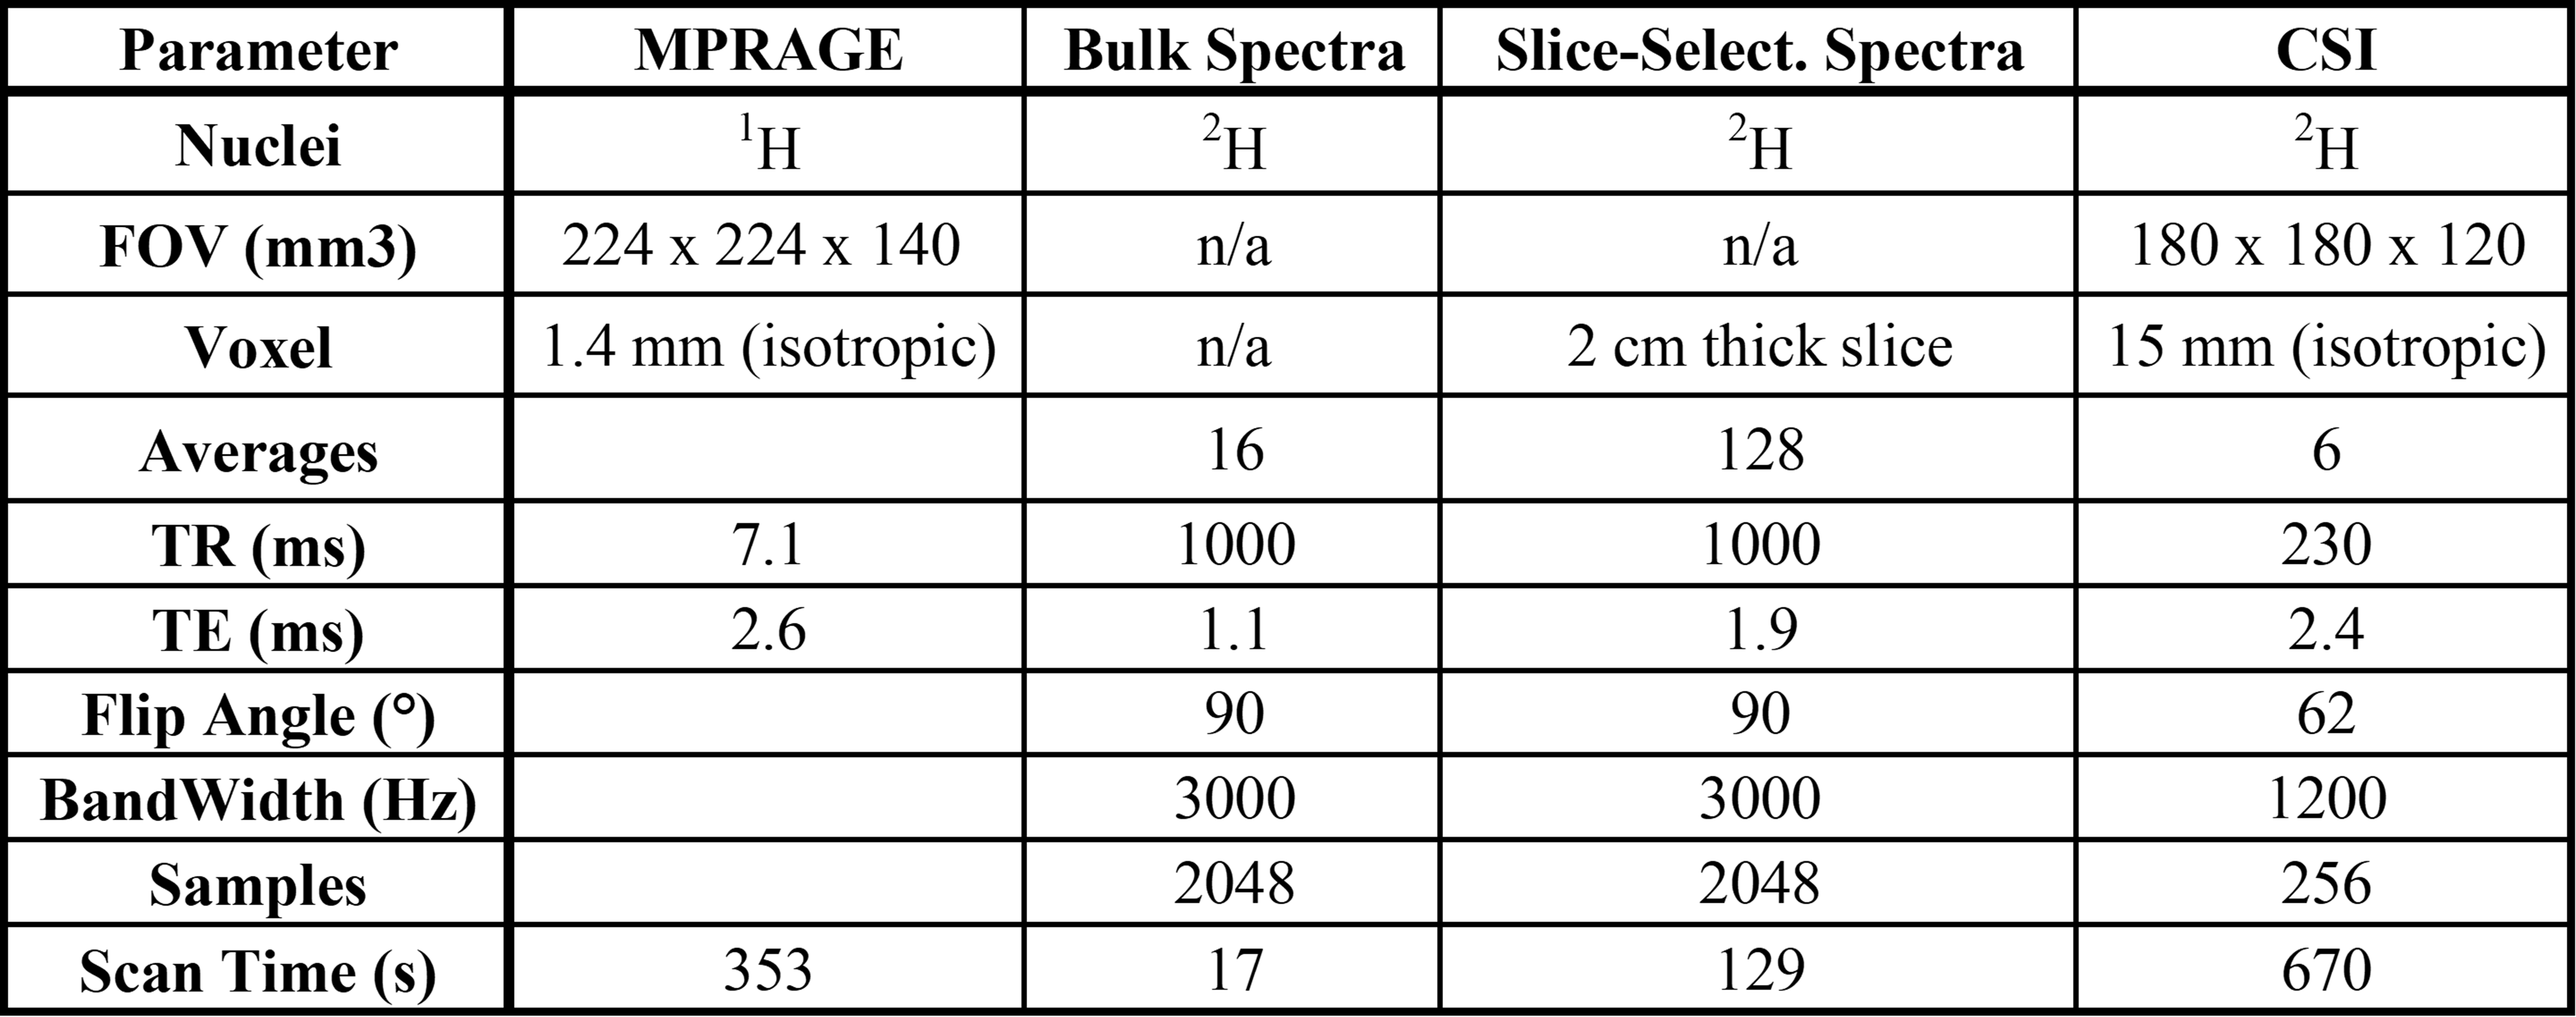
\includegraphics[width = 1\textwidth]{Figures/Glucose/Scan_Details.png}
    \caption{\textit{The parameter details for each of the scans used in this study. Note that the averages for CSI are acquisition weighted, and that the 'Bulk' spectra is non-localised.}}
    \label{fig:Glu:Scan_Details}
\end{figure}

Scanning for each participant was split into two parts, the baseline \ac{NA} scanning before the glucose drink (lasting approximately 20 minutes) which was used for quantification and calibration, and the 90-minute scanning session after the glucose drink was ingested. The drink was consumed in a maximum of eight minutes. Baseline measurements included a $^1$H scout scan for planning; a $^1$H \ac{MPRAGE} scan (\ac{FOV}: 224 x 224 x 140 mm$^3$, 1.4 mm isotropic voxels, \ac{TR}: 7.1 ms, \ac{TE}: 2.6 ms, T$_\text{scan}$: 353 s); a non-localised $^2$H spectrum (16 averages, \ac{TR}: 1000 ms, \ac{TE}: 1.1 ms, $\alpha$: 90$^\circ$, \ac{BW}: 3000 Hz, 2048 samples, with a scan duration of 17 s); a slice-selective $^2$H spectra, acquired from a 2-cm-thick axial slice positioned over the lateral ventricles, using 128 averages, TR: 1000 ms, TE: 1.9 ms, $\alpha$: 90$^\circ$, \ac{BW}: 3000 Hz,  2048 samples with a T$_\text{scan}$: 129 s and a 3D $^2$H \ac{CSI} covering the whole brain (\ac{FOV}: 180 x 180 x 120 mm$^3$ , 15 mm isotropic voxels, \ac{TR}: 230 ms, \ac{TE}: 2.4 ms, $\alpha$: 62$^\circ$, \ac{BW}: 1200 Hz, 256 samples, with a T$_\text{scan}$: 670 s) acquired using 6 acquisition-weighted \cite{Pohmann2001AccurateCSI} averages. All the \ac{NA} scans were performed in the absence of visual stimulation and after these data were acquired the participant was then brought out of the scanner and consumed the glucose drink. This contained 0.75g/kg (bodyweight) of either D$_2$ or D$_7$-glucose powder purchased from CK Isotopes Ltd. (microbiological/pyrogen-tested product) and Merck Life Science UK Ltd. (endotoxin-tested product) dissolved in 250 ml of water at room temperature. The participant was allowed to consume this in their own time, and when they indicated that they were ready for the second scanning session ($\sim$30 minutes later), were guided back into the scanner.

\begin{figure}
    \centering
    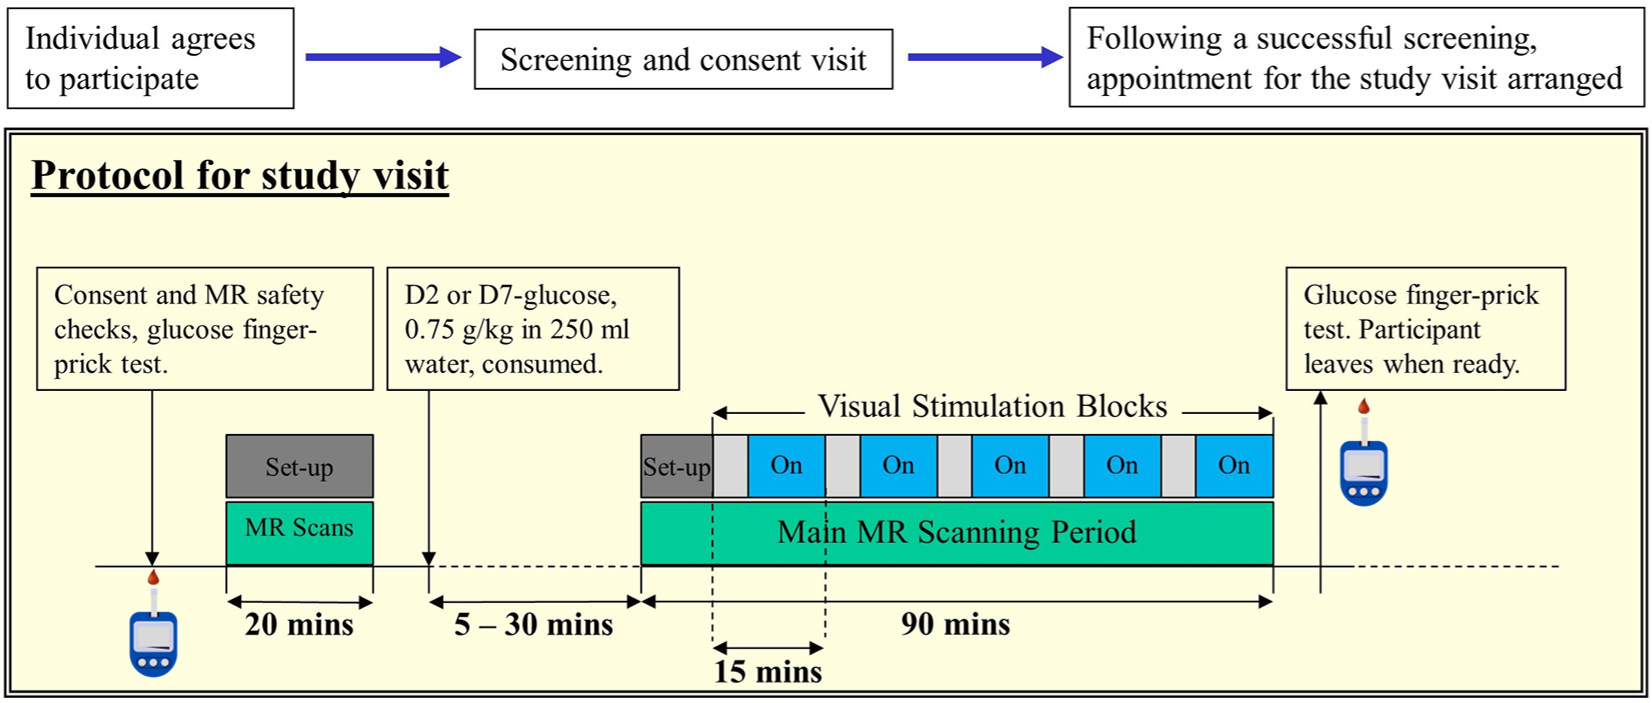
\includegraphics[width = 1\textwidth]{Figures/Glucose/Protocol.png}
    \caption{\textit{Schematic of the scanning protocol that was used in this study. Above the box the three main steps for recruitment are outlined, inthe yellow box the details of the study day are listed. The study day starts with a blood-glucose test before \ac{NA} and post ingestion scanning.}}
    \label{fig:Glu:Protocol}
\end{figure}

In the second session, the two $^1$H scans were repeated, followed by five or six repeats of the three $^2$H scans. In the event that the participant needed to exit the scanner for a short period and re-enter, the $^1$H scans were repeated before continuing with the $^2$H scans. If the participant was to be visually stimulated, the display was activated during the \ac{CSI} scans only and quiescent otherwise.  

Visual stimulation was produced via an 8 Hz flashing, black and white, radial checkerboard, similar to what has been used previously \cite{Fernandes2020MeasurementT}. The visual display was projected onto a screen that the participants could observed by wearing prism glasses while lying in the scanner. Most of the participants who experienced visual stimulation (three that ingested D$_2$-glucose and four that ingested D$_7$-glucose) were shown a checkerboard flashing pattern that was active for 50 seconds followed by 10 seconds of rest (red cross on a grey background). However, two participants (both of whom ingested D$_2$-glucose) experienced a checkerboard flashing pattern that was active for 30 seconds followed by 30 seconds of a red cross on a grey background. Participants who received no visual stimulation were asked to close their eyes during the scanning session. In all cases, the scanner room lights were turned off. 

\subsection{Image and spectral processing}

\begin{figure}
    \centering
    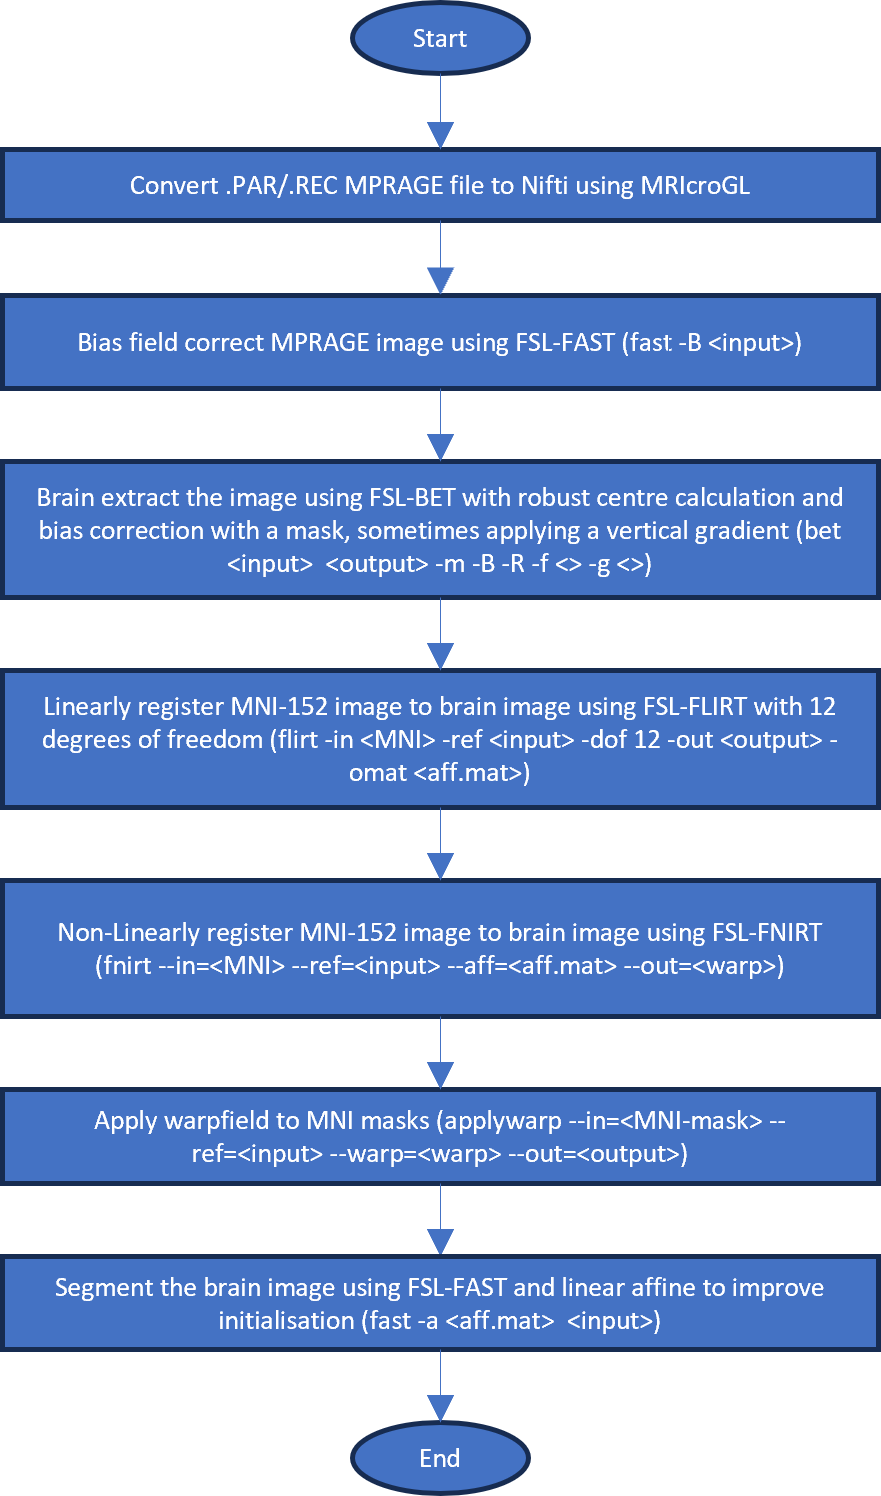
\includegraphics[width = 0.8\textwidth]{Figures/Glucose/Flow_Image.png}
    \caption{\textit{Flowchart outlining the steps used to analyse the $^1$H MPRAGE images and obtain the \ac{ROI} Masks. The case-sensitive FSL commands are included in brackets.}}
    \label{fig:Glu:1H_Flow}
\end{figure}

The $^1$H \ac{MPRAGE} images were converted to a NIFTI format using MRIcroGL (www.nitrc.org), and bias-field corrected using FSL-FAST \cite{Zhang2001SegmentationAlgorithm}. Each corrected \ac{MPRAGE} image was then brain extracted using FSL-BET \cite{Smith2002FastExtraction} which also bias-field-corrected the image and removed any neck voxels. The fractional intensity threshold was allowed to vary between subjects along with the gradient in the foot-head direction. This was done to ensure the brain extraction was optimised for each participant. The MNI-152 brain image dataset with 2 mm isotropic voxels (distributed with FSL \cite{Smith2004AdvancesFSL}) was linearly registered to each image using FSL-FLIRT \cite{Jenkinson2001AImages, Jenkinson2002ImprovedImages} and twelve degrees of freedom. The MNI-152 brain image was then non-linearly registered to the same image to obtain the warp-field using FSL-FNIRT \cite{AnderssonJ2008FNIRT-FMRIBsTool}, with the affine matrix from the linear registration used as an initial guess. The warp-field was then used to non-linearly register probabilistic maps of the frontal and occipital lobes from the MNI-152 atlas to the \ac{MPRAGE} space. The maps were subsequently binarised to obtain \ac{ROI} masks. These regions were chosen to test whether contrast in metabolite signals/concentrations could be detected with participants who were visually stimulated. A flowchart that outlines the analysis steps for the $^1$H MPRAGE images and the construction of the masks can be seen in Fig. \ref{fig:Glu:1H_Flow}.

%  \ac{CSF}, \ac{GM} and \ac{WM} could also be obtained using FSL-FAST \cite{Zhang2001SegmentationAlgorithm}, however it as deemed the resulting masks were not accurate representations of the tissue.

% The below is not done anymore:
% Finally, FSL-FAST \cite{Zhang2001SegmentationAlgorithm} is used on the brain-extracted \ac{MPRAGE} image to form probabilistic maps for \ac{CSF}, \ac{GM} and \ac{WM}, with the affine matrix used to improve initialisation. The \ac{CSF} mask was manually segmented to only include the left and right ventricles

A noise spike that affected each voxel at the same frequency position was visible. In some of the spectra the spike which generally only affected one data point in each spectrum most likely arose from baseline error. To correct this spike the data points on either side of corrupted point were averaged together and the spike was replaced with this value. 

\begin{figure}
    \centering
    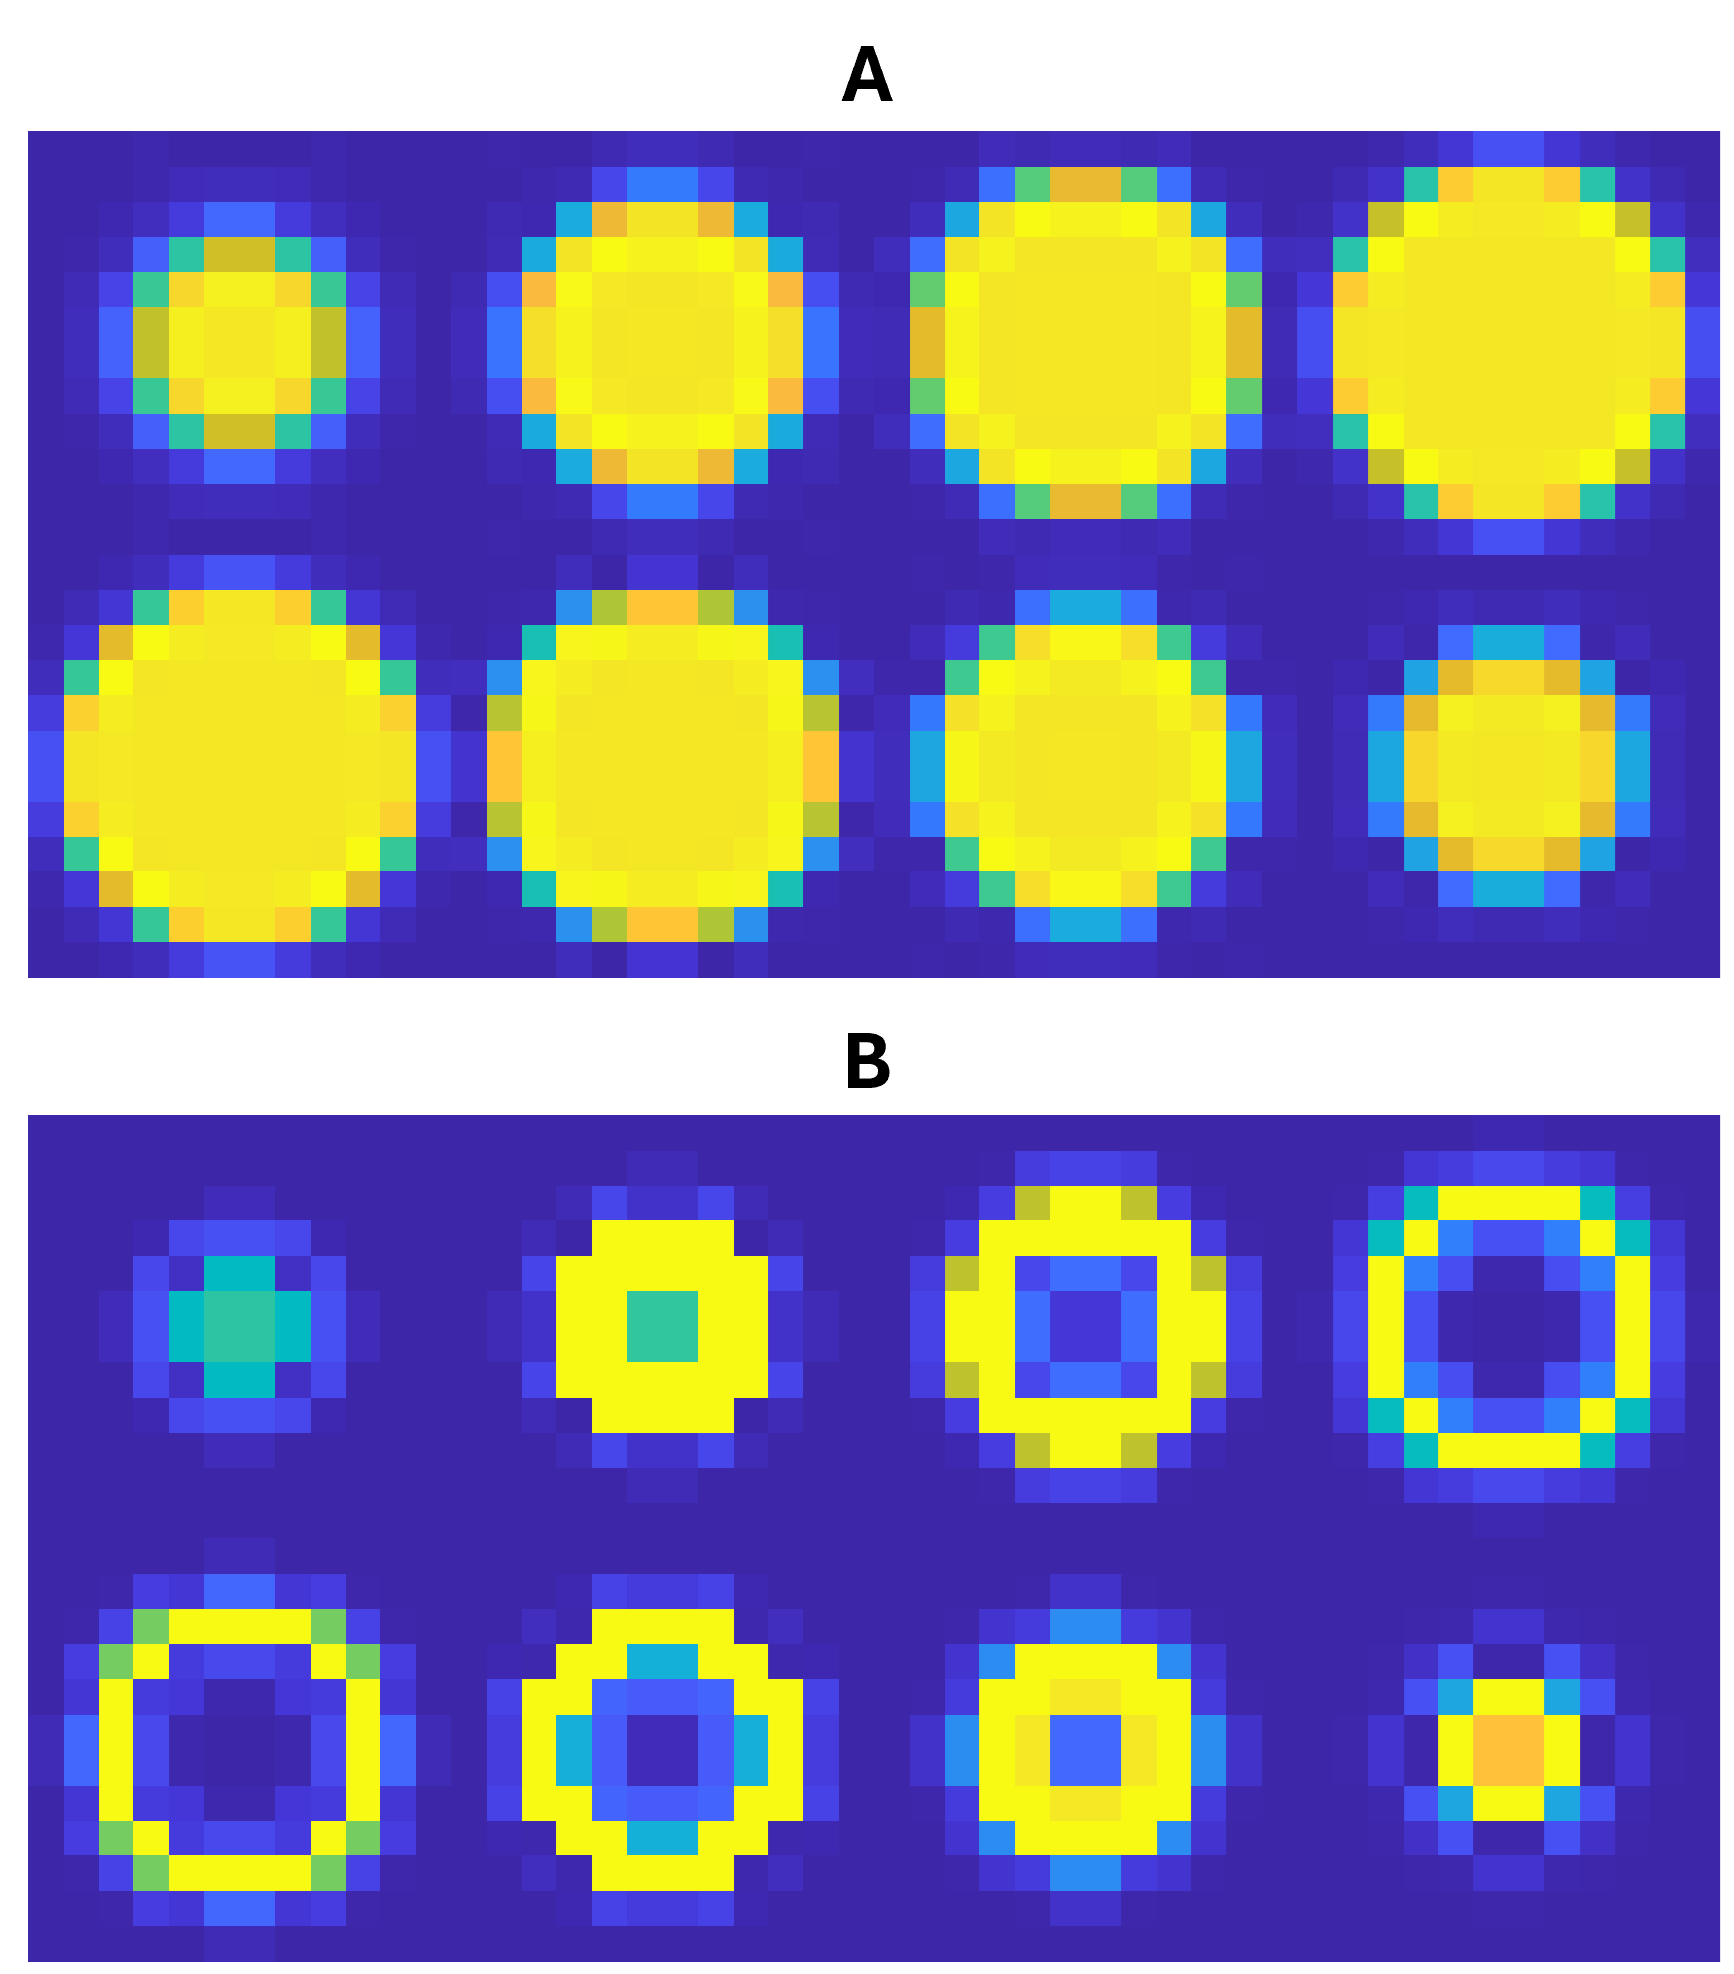
\includegraphics[width = 0.6\textwidth]{Figures/Glucose/Template.png}
    \caption{\textit{3D simulated spherical (A) and hollow-spherical (B) signal distributions used to simulate \ac{DMI} data, for testing different core matrix sizes when de-noising.}}
    \label{fig:Glu:Temp}
\end{figure}

Apodisation and smoothing techniques have been shown to affect metabolite quantification in \ac{MRSI} \cite{Goryawala2020EffectsFitting}, which is why it was chosen to not apodise when analysing the data. Low-rank denoising has been shown to be able to use the similarities in temporal/spatial information to denoise, better than for single voxel denoising \cite{Brender2019DynamicHyperpolarization, Goryawala2020EffectsFitting}. Tucker decomposition also known as a \ac{HOSVD} is an extended version of the simpler \ac{SVD}, which is then followed by a low rank approximation. Here only the largest singular values persist, and the rest are replaced with zeros, therefore when reconstructed the data is similar except only the most prominent features persist. This works as a de-noising method as the noise will be represented as smaller singular values and will hence be removed, only leaving the metabolite peaks as described in section \ref{Chap:Theory:denoise}. This can be performed in either the frequency or the time domain. 

\begin{sidewaysfigure}
   \centering
   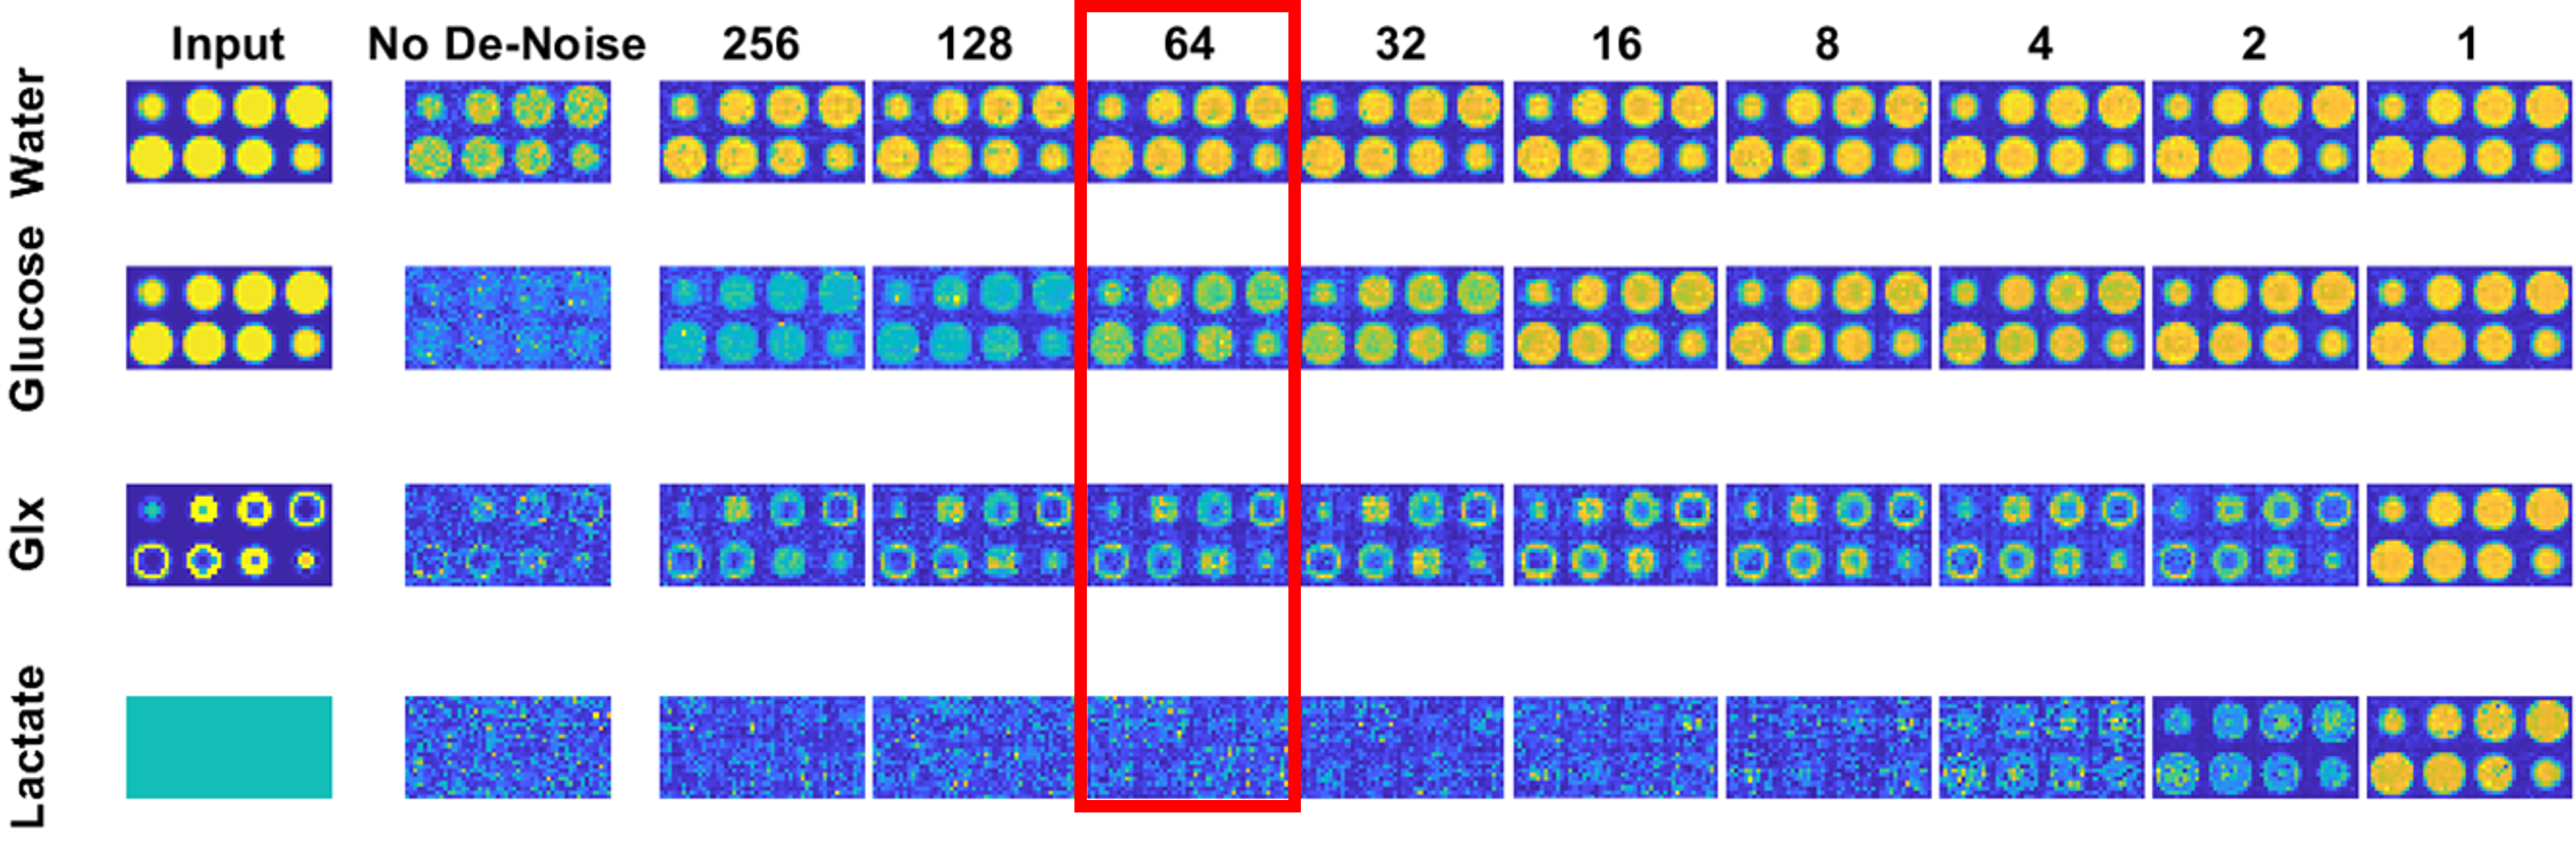
\includegraphics[width = 0.95\textwidth]{Figures/Glucose/DeNoise_Sim.png}
   \caption{\textit{Ground truth signal distributions for $^2$H water, glucose and Glx (far left) followed by amplitudes obtained from fitting spectra to varying levels of compression in the \ac{FID} sampling direction. The spatial dimensions are compressed to a core matrix size of [6 6 4]. The red box shows the choice of compression for the FID sampling direction, the spectral \ac{SNR} of the centre region $\sim$7.5.}}
   \label{fig:Glu:DeNoise}
\end{sidewaysfigure}

Here, each \ac{CSI} data-set was denoised in the time-domain using a Tucker decomposition \cite{Bader2007EfficientTensors} with a compression matrix size of [64 6 6 4] (spectral and 3 spatial dimensions). The core matrix size was chosen by simulating 3D \textit{in vivo} $^2$H \ac{CSI} spectra for HDO, glucose and Glx resonances. To reflect the form of \textit{in vivo} data, the amplitude distribution for water and glucose followed a spherical pattern (Fig. \ref{fig:Glu:Temp}A) whilst the amplitude distribution for Glx followed a hollow-sphere (Fig. \ref{fig:Glu:Temp}). Then by varying the core matrix size in a single direction (whilst keeping the others the same) and fitting the spectra, it is possible to compare the signal distribution for each metabolite at each compression size. An example of this can be seen in Fig. \ref{fig:Glu:DeNoise} as the dimensions of the core matrix in the FID sample direction are varied, with the amplitudes for HDO, glucose and Glx being displayed. A choice is then made for the compression in the selected direction that does not modify the overall distribution for each metabolite whilst still de-noising the data. This is then repeated for each of the other spatial directions until an optimal compression matrix size is obtained. The resulting compression matrix size (relative to total data size) is similar to compression matrix sizes that have been previously used with \ac{DMI} \cite{vonMorze2021ComparisonT, Kreis2020MeasuringMRI} and $^{13}$C studies \cite{Brender2019DynamicHyperpolarization}. The effect of de-noising using a Tucker decomposition with this core matrix size can be seen in Fig. \ref{fig:Glu:DeNoise_spectra}.

\begin{figure}
   \centering
   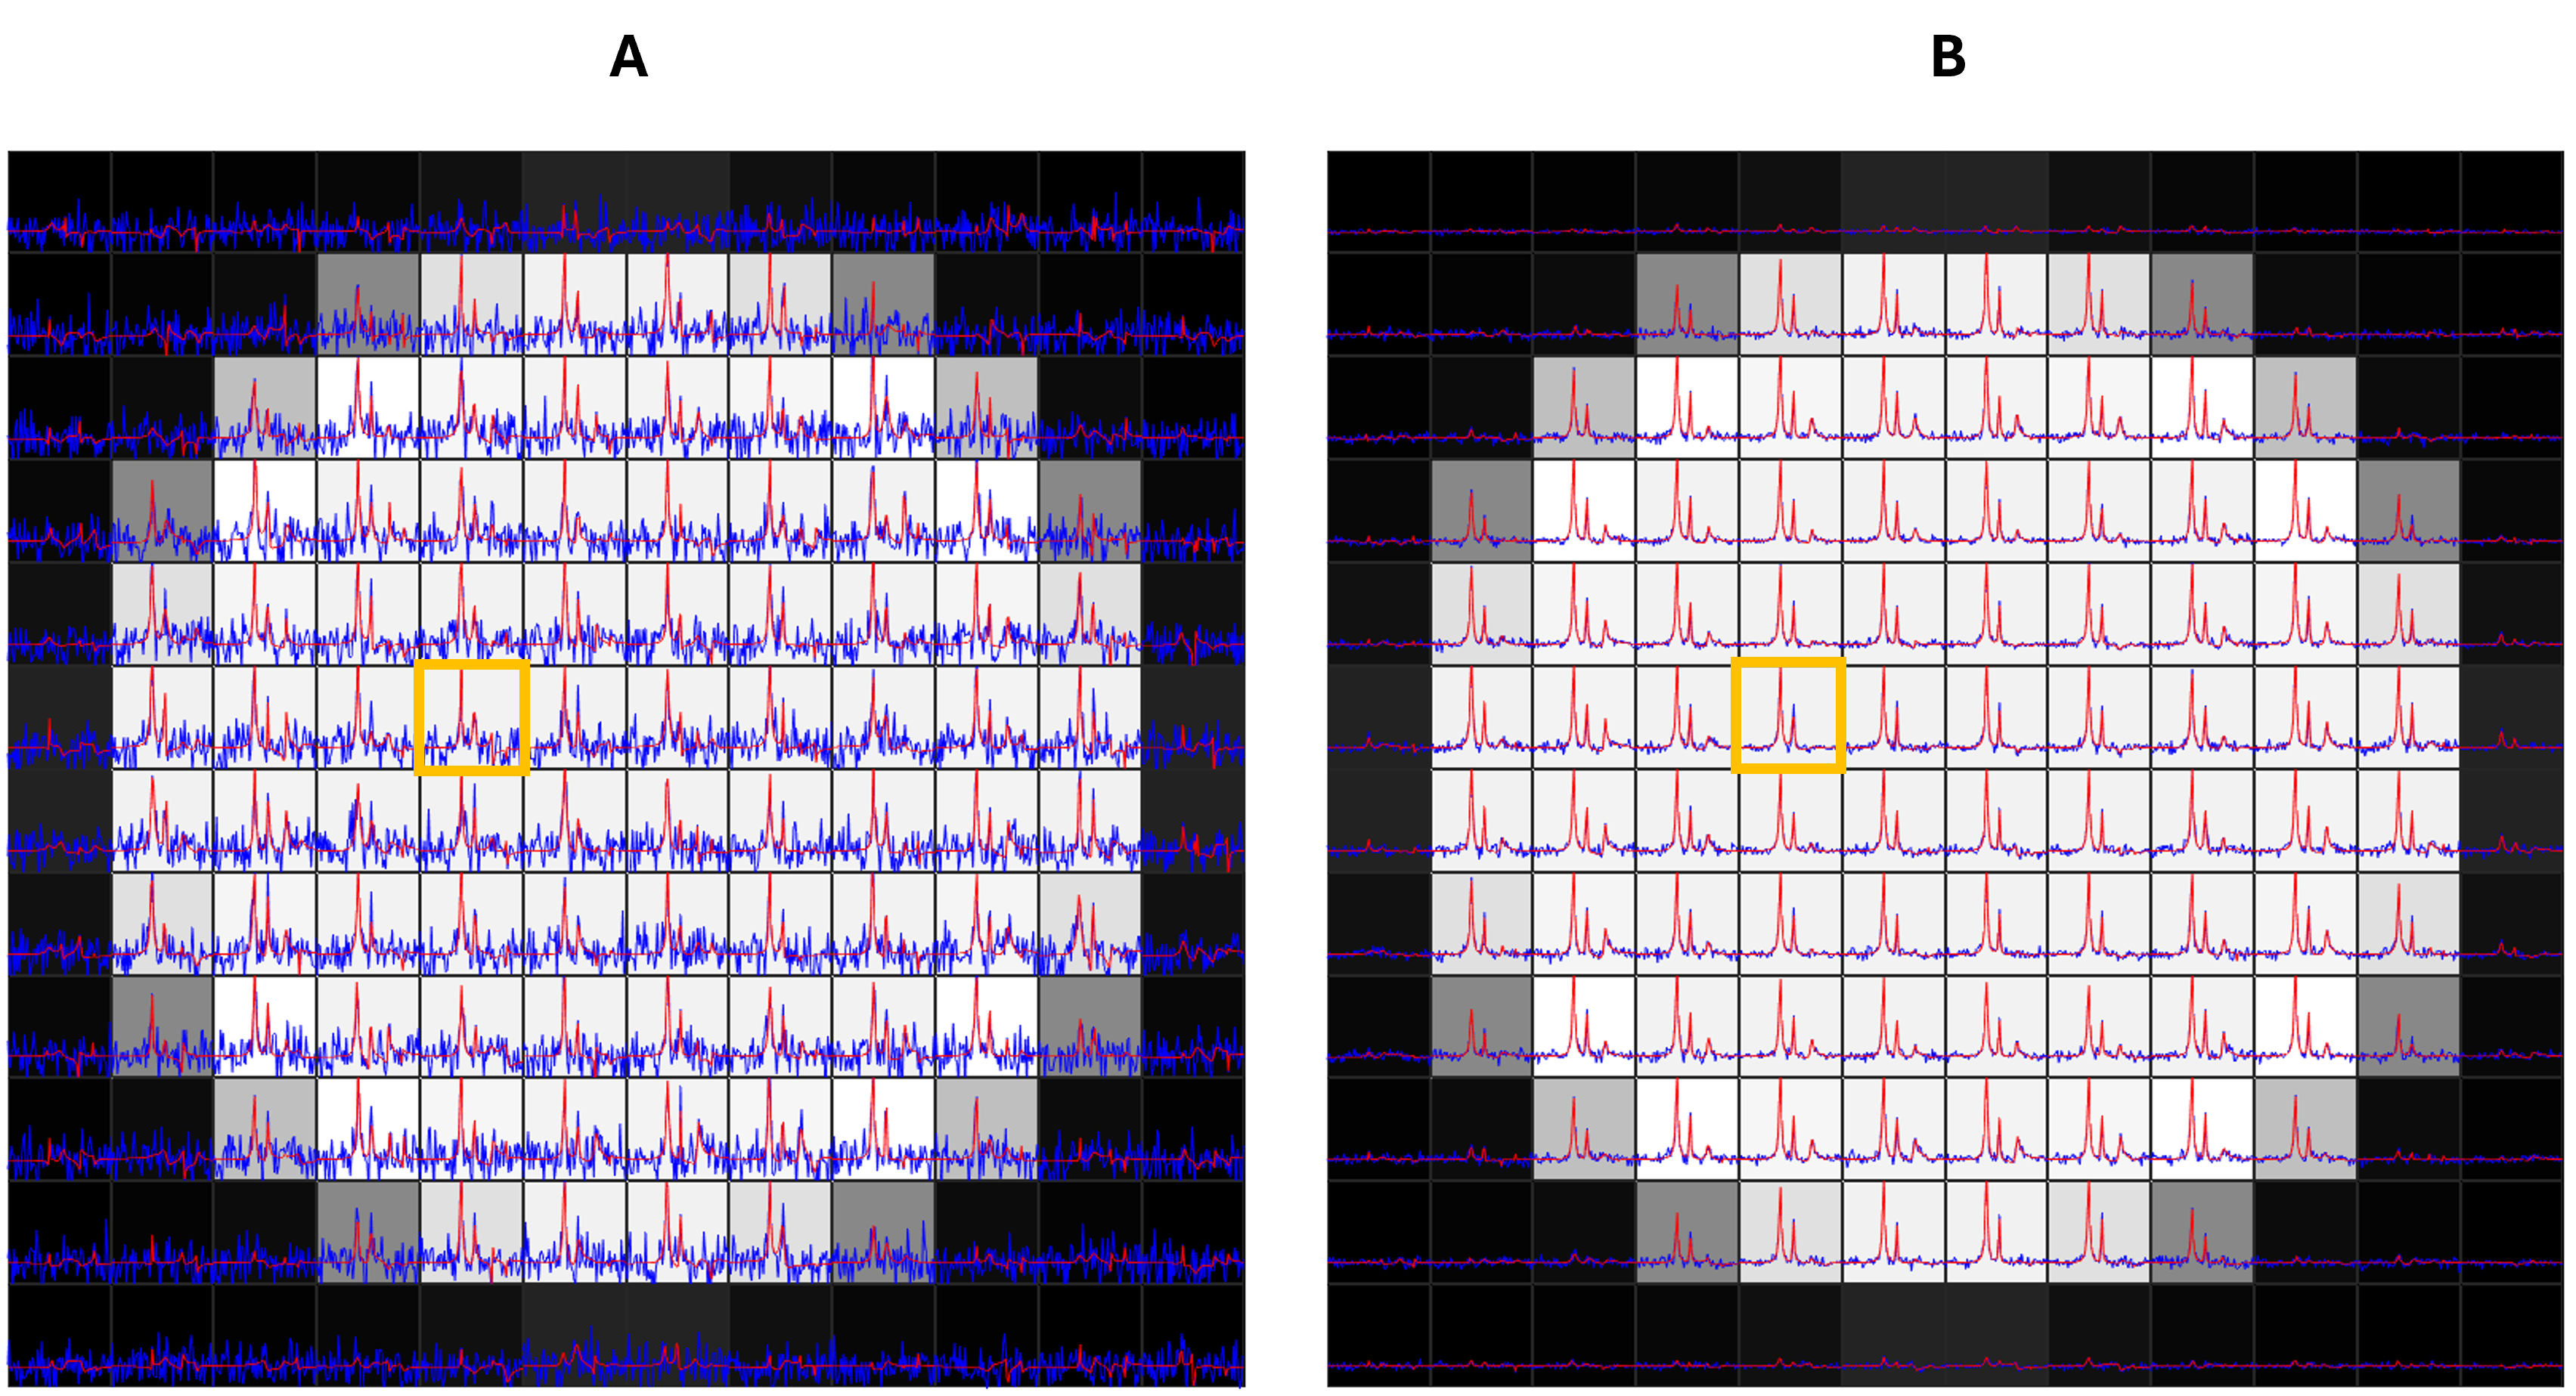
\includegraphics[width = 1\textwidth]{Figures/Glucose/DeNoise_Spectra.png}
   \caption{\textit{\ac{CSI} simulated data (blue) and the corresponding fits (red) for a single slice overlayed onto the sphere from Fig. \ref{fig:Glu:Temp}A. A is the results before de-noising and B is the results after a Tucker decomposition with a core matrix of [64 6 6 4]. Here the \ac{SNR} in the highlighted voxels increases from $\sim$7.5 to $\sim$16.5.}}
   \label{fig:Glu:DeNoise_spectra}
\end{figure}

With low \ac{SNR} datasets it can be possible to bias the data using de-noising. One way to overcome this is to simulate your data and apply varying levels of de-noising which can help choose rank reduction. This was performed with our dataset which helped motivate the choice of rank reduction, which is why de-noising was only applied to each \ac{CSI} and not in addition with a fifth domain of time. It was found that any level of de-noising in this domain smoothed the metabolite change curves, when compared to individual \ac{CSI} de-noising. To avoid biasing the lactate peak (because of its low \ac{SNR}) the simulated data had no true lactate peak present, therefore any presence of lactate above the noise floor in the amplitude maps would indicate too much of a rank reduction. It was found that a rank of eight in the spectral domain and ranks below four in the spatial domain were too small. This can be seen in Fig. \ref{fig:Glu:DeNoise}.

\begin{table}[H]
    \centering
    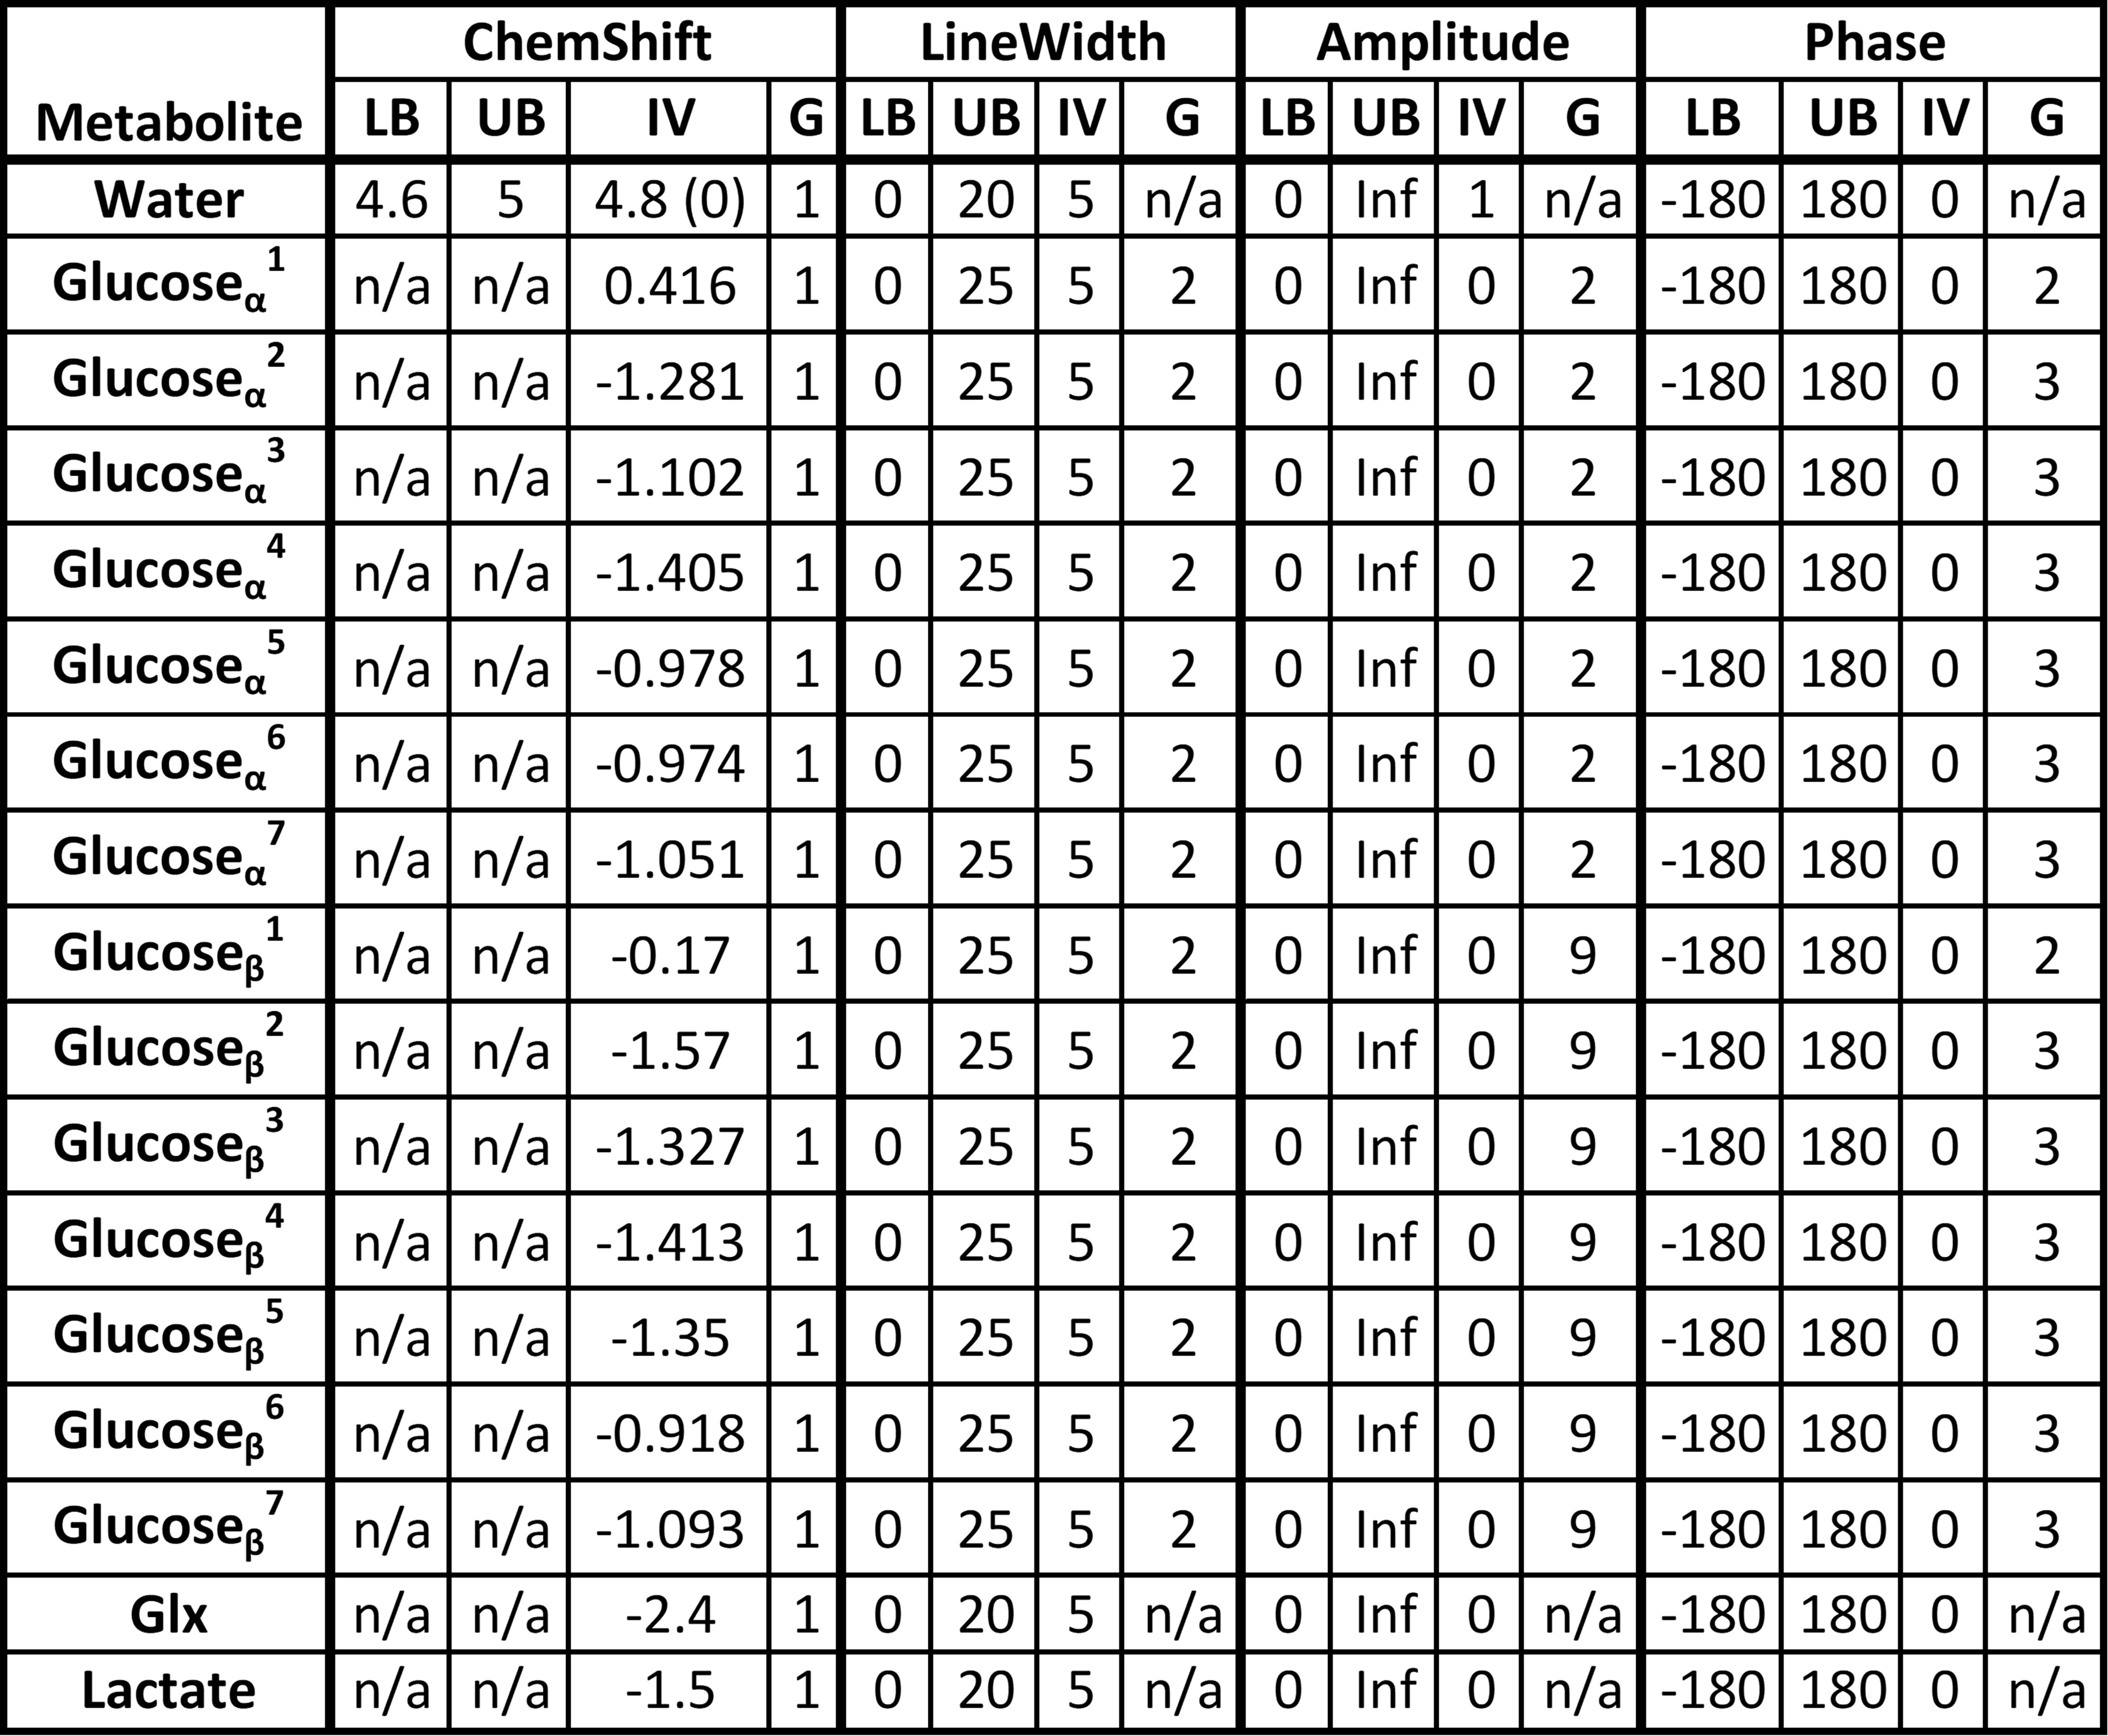
\includegraphics[width = 1\textwidth]{Figures/Glucose/Prior_Table.png}
    \caption{\textit{Prior knowledge used in OXSA-AMARES \cite{Vanhamme1997ImprovedKnowledge, Purvis2017OXSA:MATLAB} to fit the individual \ac{CSI} datasets after D$_7$-glucose ingestion, which includes the parameters chemical shift, linewidth, amplitude and phase. The acronyms are defined as LB:Lower-Bound, UB:Upper-Bound and IV:Initial-Value. N/a refers to non-applicable meaning the parameter is not used with this metabolite, this is because it is grouped to something else or is not grouped to any other metabolite. The `G' column shows which peaks are grouped for each parameter.}}
    \label{fig:Glu:Prior}
\end{table}

The \ac{FID}s were fitted using an adapted version of the OXSA-AMARES MATLAB toolbox \cite{Vanhamme1997ImprovedKnowledge, Purvis2017OXSA:MATLAB}, which requires prior knowledge for each of the metabolites, the values used for D$_7$-glucose can be seen in Table \ref{fig:Glu:Prior}. In previous studies that have used D$_2$-glucose ingestion, the glucose spectrum has been fitted as a single peak at 3.8 ppm, since the chemical shift difference between the multiple resonance lines are usually not discernible due to the relatively broad linewidths and low SNR. However, this is not the case for D$_7$-glucose \cite{Govindaraju2000ProtonMetabolites} which has a larger number of spectral lines with a larger range of chemical shifts. Therefore, the spectrum needs to be modelled more accurately, taking into account the contribution from each deuterium label for both anomers ($\alpha$ and $\beta$). The chemical composition of the glucose stays the same for the different anomers, but the location of the hydroxyl group can swap with the $^1$H on C1. When dissolved in water 1/3 of glucose will exist in the $\alpha$ form whilst 2/3 will exist in the $\beta$ form \cite{Leitch2009-Erythrocytes}.

Here, the glucose signal is fitted as a sum of 14 peaks due to the number of label positions for both anomers. For consistency, this approach was also implemented when analysing the D$_2$-glucose data, which resulted in 4 lines being fit for the glucose signal. The $^2$H chemical shifts of the glucose, Glx, and lactate resonances are assumed to be the same as those of the $^1$H chemical shifts \cite{Govindaraju2000ProtonMetabolites} and were implemented in the fitting as relative shifts to the water peak \cite{Meerwaldt2023InImaging}. The glucose peaks were fitted assuming a common scaling factor; all glucose peaks have the same phase, other than the peaks from the C1 position which have a different phase due to large differences in chemical shift. The linewidths of peaks from the same anomer share the same value. For \ac{HDO}, Glx, and lactate, only single components were assumed, with independent amplitudes, phases, and linewidths.

\begin{figure}
    \centering
    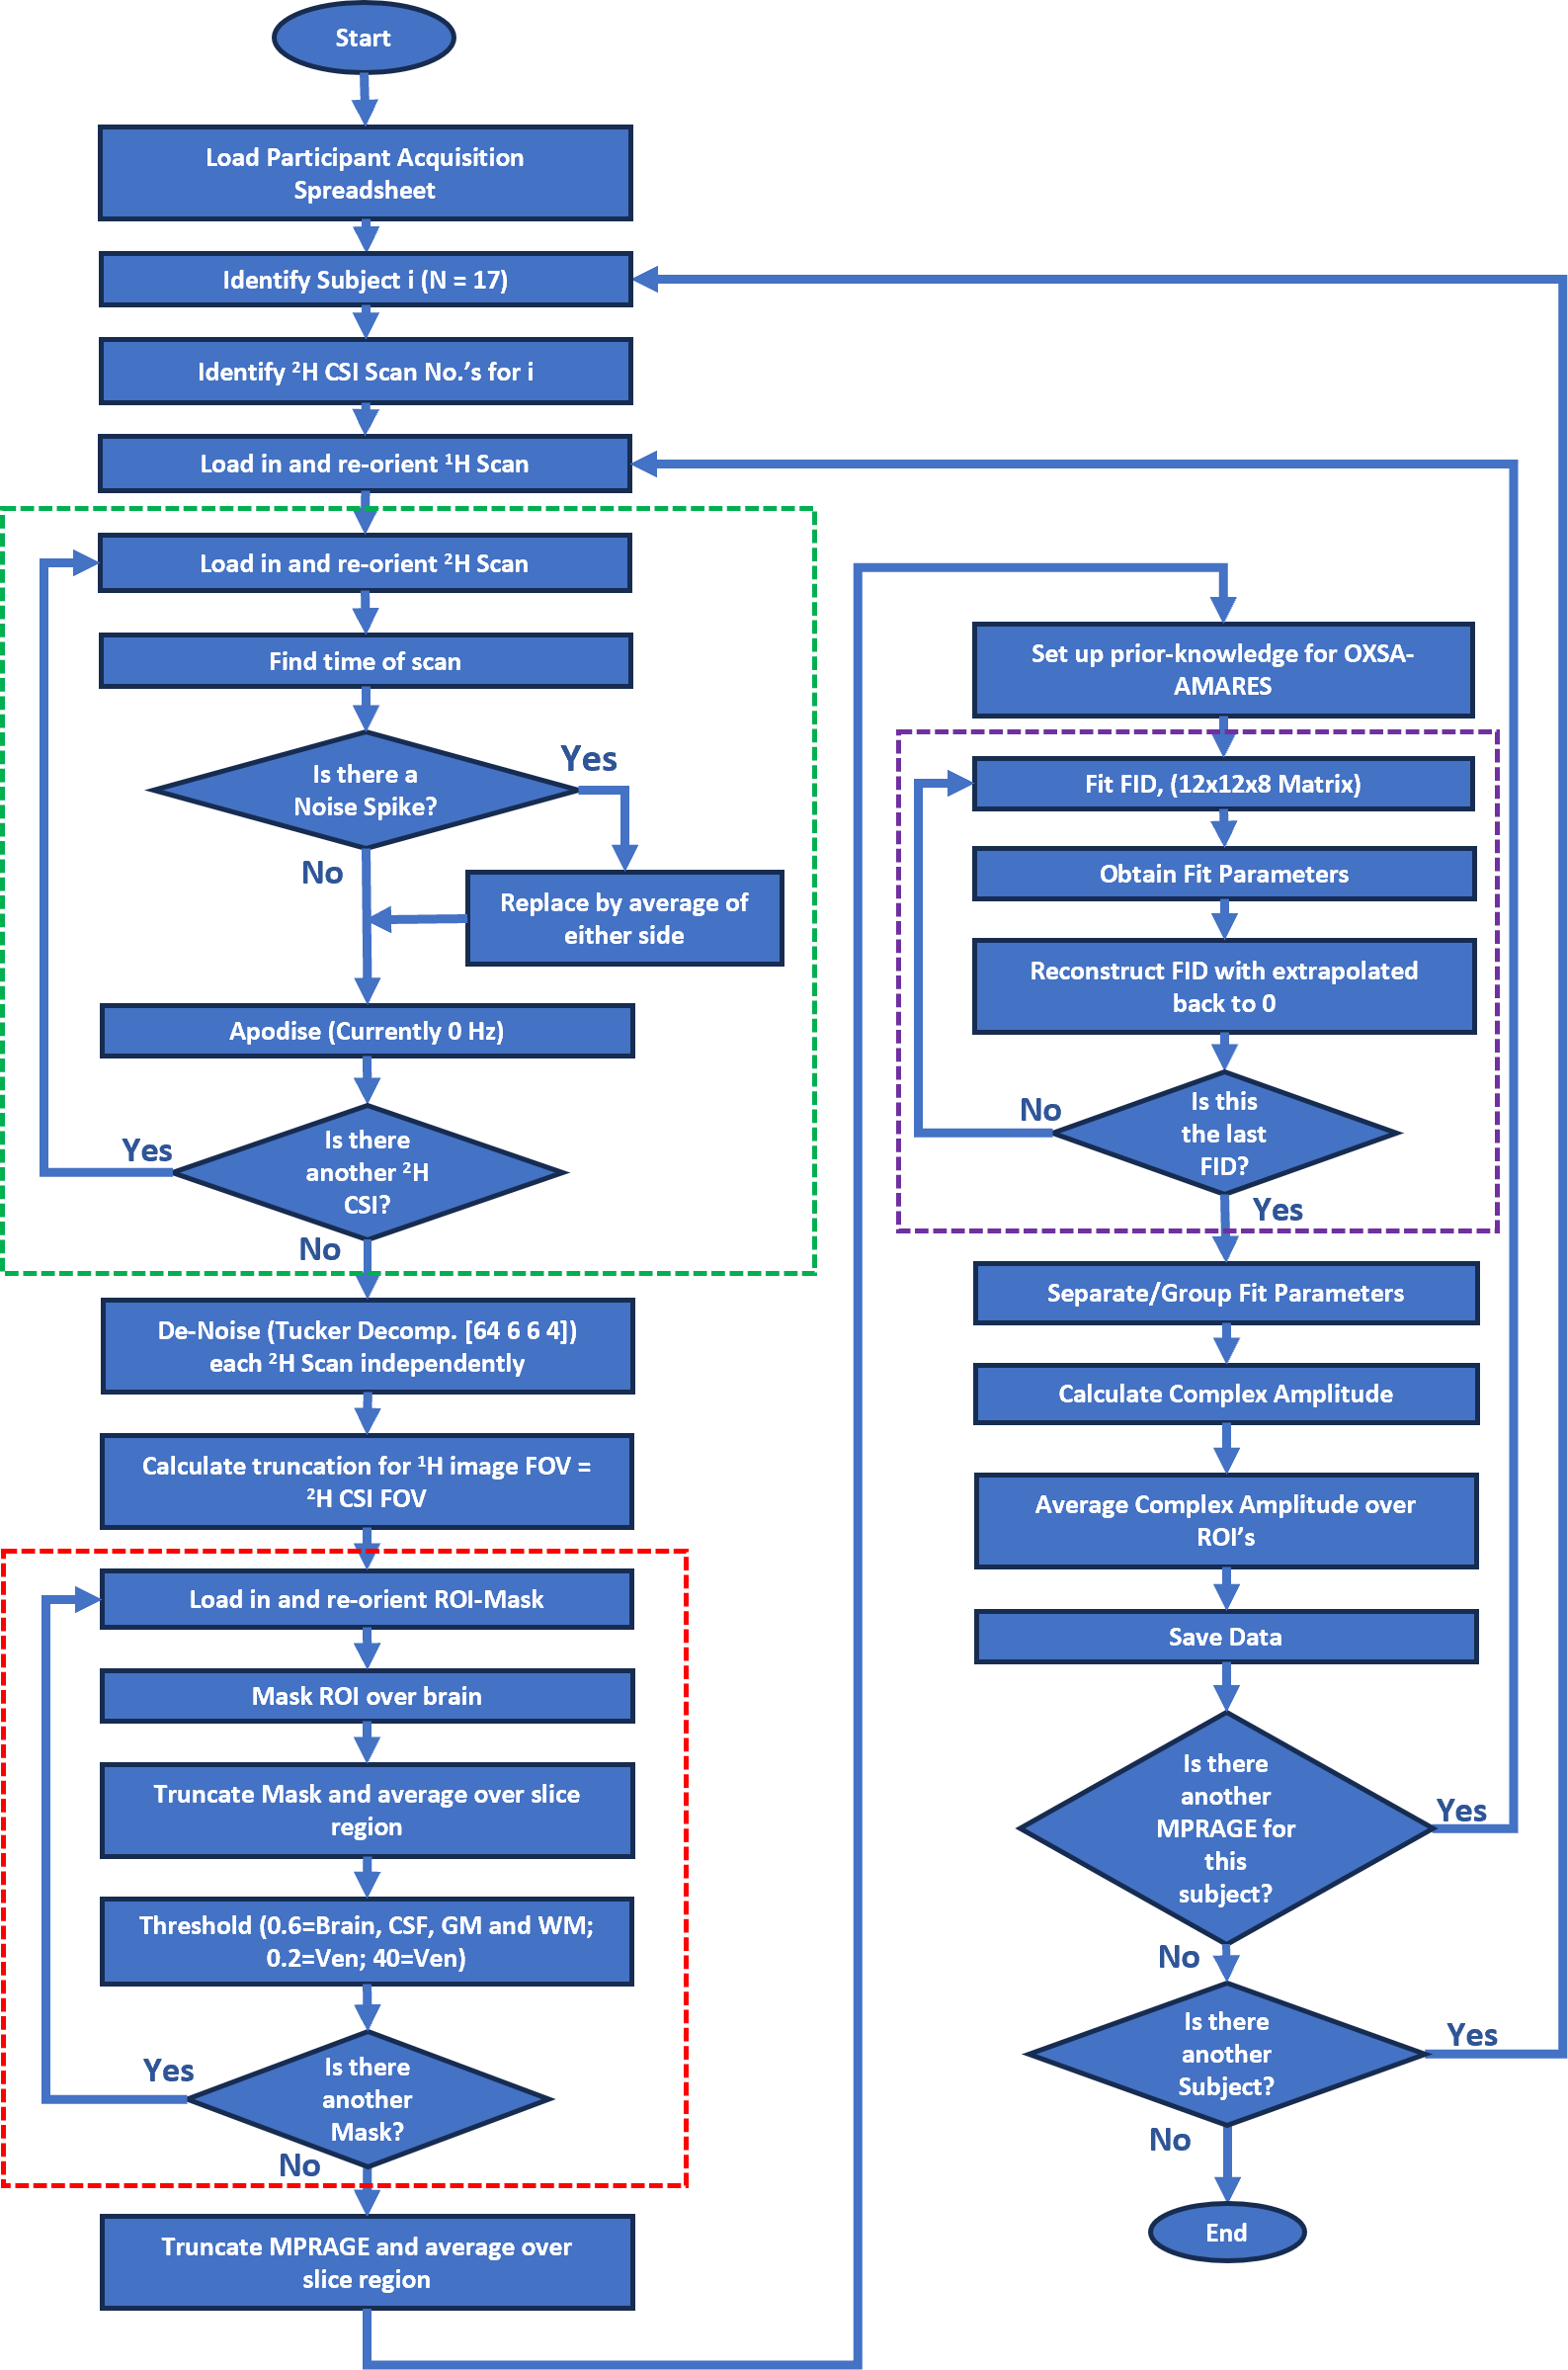
\includegraphics[width = 0.9\textwidth]{Figures/Glucose/2H_Flow.png}
    \caption{\textit{Flowchart outlining the steps used to analyse the $^2$H \ac{CSI} spectral data (including de-noising). The dotted green box represents the pre-processing steps for the $^2$H data, the dotted red box describes the application of the $^1$H mask and the dotted purple box describes the fitting of each spectra.}}
    \label{fig:Glu:2H_Flow}
\end{figure}

Due to the additional prior knowledge the fitting routine takes approximately 2 to 3 times longer for the D$_7$-glucose analysis compared to the D$_2$-glucose analysis, the exact times can vary depending the SNR for each metabolite during the time-course, appproximate average time per spectrum to obtain fit parameters for D$_2$- and D$_7$-glucose \ac{CSI} data respectively are $\sim$0.16 s and $\sim$0.32 s (with default optimisation). The increased complexity of the fitting means it is less likely to accurately fit the \ac{FID} however by narrowing the linewidth constraints and using more accurate initial estimates, as well as lowering the tolerance of the fit (increasing iterations and function evaluations and lowering the function and step tolerance) the fit is found to overlay the data accurately as seen in Figs. \ref{fig:Glu:Select} and \ref{fig:Glu:Avg_Amp}. 

\begin{figure}
    \centering
    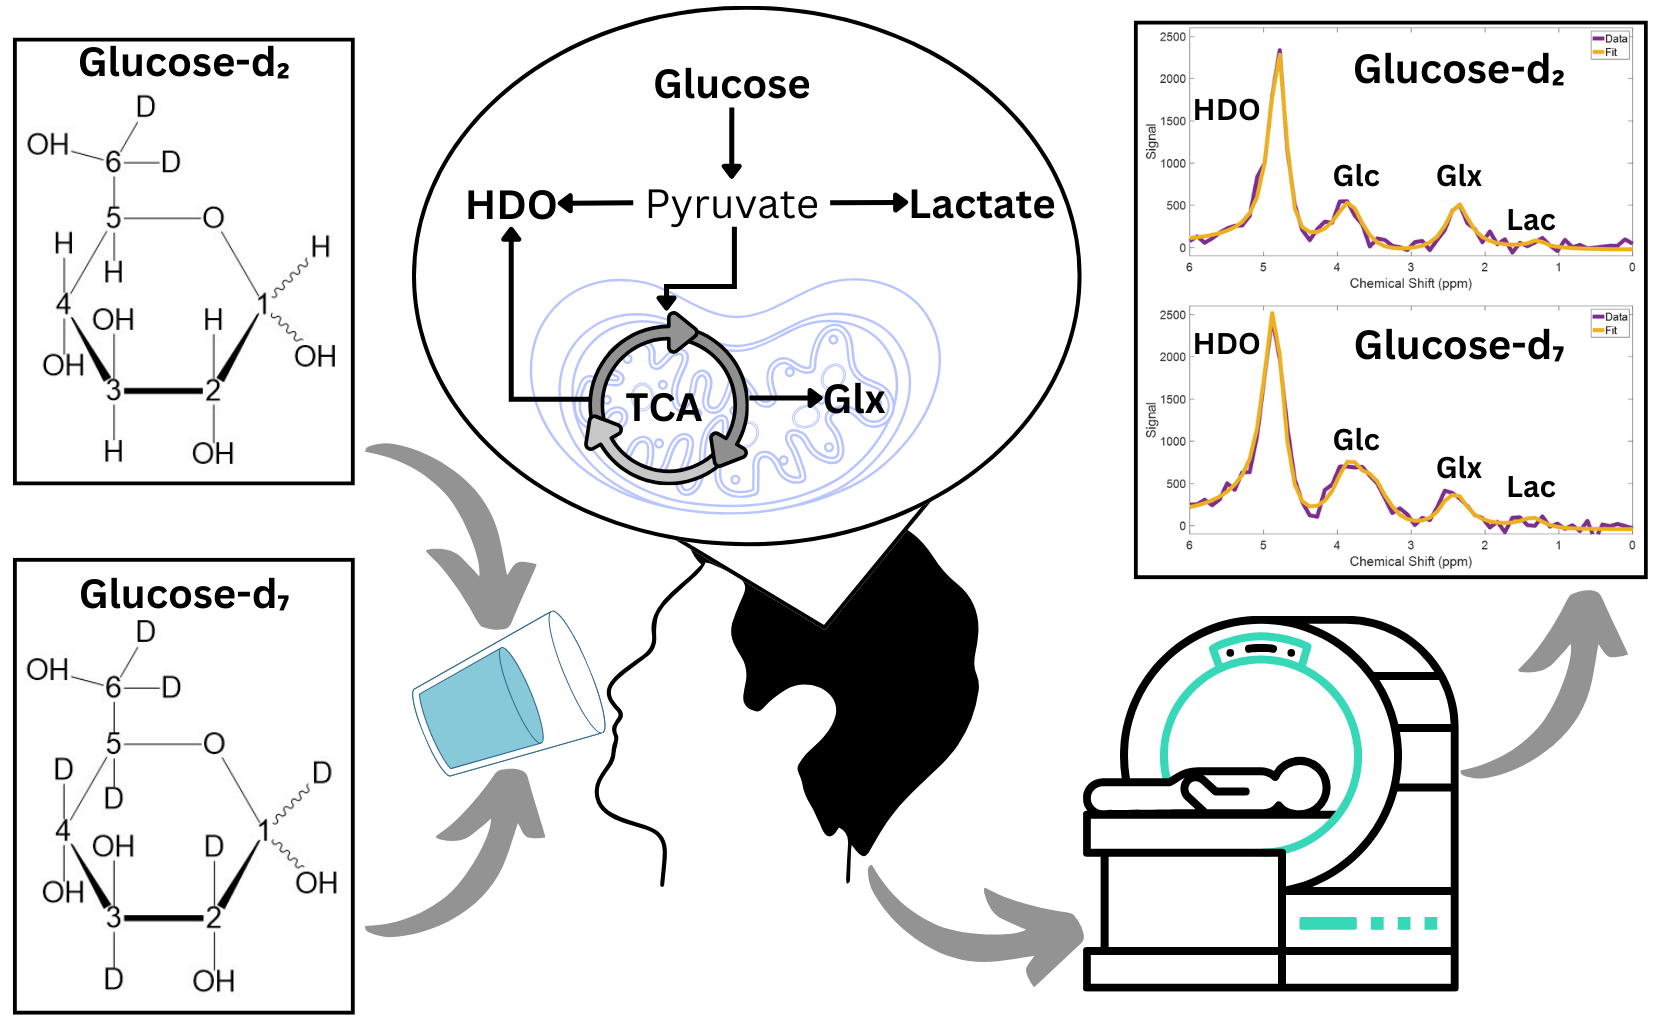
\includegraphics[width = 1\textwidth]{Figures/Glucose/Study_Day.png}
    \caption{\textit{Schematic diagram of the approach used to obtain the $^2$ MRSI data in this study.}}
    \label{fig:Glu:Study_Day}
\end{figure}

The amplitude and phase values for each metabolite peak at each voxel position were converted to complex amplitudes and interpolated to the same resolution as the \ac{MPRAGE} image. These maps were then averaged over the whole-brain, occipital lobe, and frontal lobe \ac{ROI} (using the binarised segmentation maps) to obtain \ac{ROI}-averaged amplitudes for each metabolite for each \ac{CSI} data-set. This provided amplitude time-courses as a function of time relative to glucose ingestion. These values were then either quantified into concentration values, normalised or corrected for the effect of T$_1$ differences and used as ratios between the two different types of glucose. A flowchart that outlines the steps used to analyse all the $^2$H \ac{CSI} data can be seen in Fig. \ref{fig:Glu:2H_Flow}.

\subsection{Concentration calculations}
\label{Chap:Glu:conc}

Concentrations $C^m$ for each metabolite $m$ were determined using the following equation

\begin{equation}
    C^m = \frac{A^m}{kE^mN^m},
    \label{eqn:Glu:Conc}
\end{equation}

where $A^m$ is the FID amplitude of the metabolite, $N^m$ is the number of effective $^2$H labels per metabolite molecule, $E^m$ is the attenuation factor given by

\begin{equation}
    E^m = \frac{1-\exp(-\text{TR}/T_1^m)}{1-\exp(-\text{TR}/T_1^m)\cos{\alpha}}
    \label{eqn:Glu:Atte}
\end{equation}

where T$_1^m$ is the longitudinal relaxation time of the metabolite, TR is the repetition time, $\alpha$ is the flip angle, and $k$ is a scaling constant. This constant, which is found to be \ac{ROI}-dependent, is calculated by using the average \ac{NA} water amplitude within a given \ac{ROI}. This was calculated from the \ac{CSI} data acquired before glucose ingestion assuming an isotopic percentage for deuterium of 0.0156\% \cite{Hagemann1970AbsoluteSMOW}, a concentration of pure water at 55.4 M, a factor of 2 because of the two hydrogen atoms in water, and an estimate of the percentage of water in each \ac{ROI}. Cortical \ac{GM} and \ac{WM} were assumed to be 84\% and 69\% water \cite{Oros-Peusquens2019AImplications}. The occipital and frontal \ac{ROI}s were assumed to be comprised of 40\% \ac{GM} and 60\% \ac{WM}, resulting in a water content of 75\%. The whole brain \ac{ROI} was assumed to be 10\% \ac{CSF}, 36\% \ac{GM}, 54\% \ac{WM}, resulting in 77\% water content.

Once $k$ had been estimated for each \ac{ROI}, metabolite concentrations were calculated via Eq. \ref{eqn:Glu:Conc}, with knowledge of the $^2$H label numbers, $N^m$. The effective number of $^2$H labels depends on whether D$_2$-glucose or D$_7$-glucose was ingested and, for Glx and lactate, also depends on label-loss. To account for label-loss, we have assumed the effective number of labels for water, glucose, Glx, and lactate is 1, 2, 1.2, and 1.7, respectively for D$_2$-glucose \cite{DeGraaf2021CharacterizationStudies}. For D$_7$-glucose, we have assumed 1, 7, 0.9, and 1.3 (estimated \cite{Funk2017TheGlucose} assuming glutamine and glutamate are present in approximately equal amounts). 

Longitudinal relaxation times for glucose, Glx and lactate were assumed to be 67 ms, 139 ms, and 297 ms, respectively \cite{DeFeyter2018DeuteriumVivo}, independent of \ac{ROI}, number of $^2$H labels, and whether D$_2$-glucose or D$_7$-glucose was the metabolic precursor. For water (\ac{HDO}), the T$_1$ relaxation times were assumed to be 510 ms, 320 ms, and 290 ms for \ac{CSF}, \ac{GM}, and \ac{WM}, respectively \cite{Cocking2023DeuteriumDosing}.

\section{Results}

\begin{figure}
    \centering
    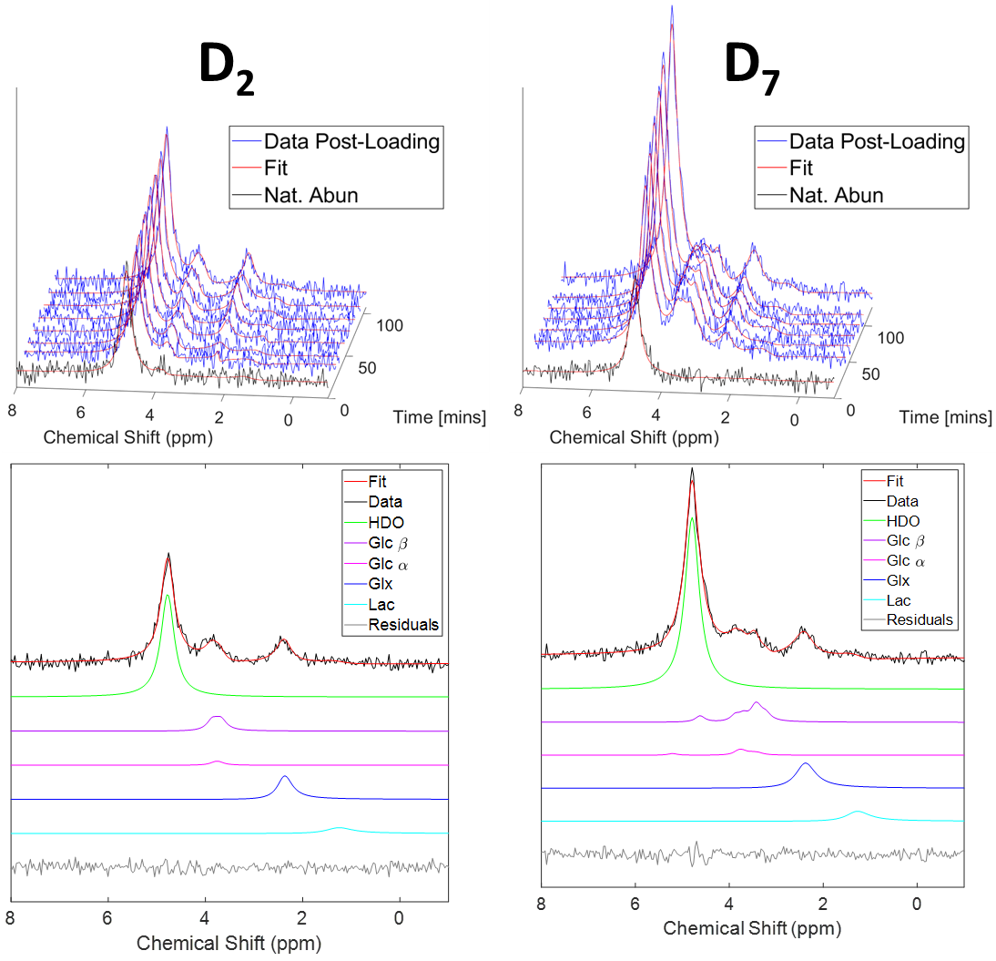
\includegraphics[width = 1\textwidth]{Figures/Glucose/Selective.png}
    \caption{\textit{Stacked selective spectra from a 2-cm-thick slice over the lateral ventricles from individual participants who had ingested D$_2$-glucose (a) or D$_7$-glucose (b). (c and d) Last spectra obtained during scanning with timepoints of $\approx$108 and $\approx$125 minutes after ingestion, for D$_2$- and D$_7$-glucose respectively. Corresponding fits are shown for each spectra, along with separated contributions from each metabolite and the residuals after fitting.}}
    \label{fig:Glu:Select}
\end{figure}

Figure \ref{fig:Glu:Select} shows spectra acquired from a 2-cm thick axial slice positioned over the lateral ventricles in two participants before and after ingestion of a similar amount per bodyweight D$_2$- or D$_7$-glucose. The spectra are displayed with the same signal intensity axis scale so that the greater amplitudes of the signals following D$_7$-glucose ingestion are evident, especially for the \ac{HDO}. Single spectra obtained $\sim$108 minutes and $\sim$125 minutes after D$_2$-glucose and D$_7$-glucose ingestion, respectively, are also shown, along with the fits, and the individual contributions to the fit from \ac{HDO}, glucose, Glx and lactate. The glucose signals include contributions from both anomers ($\alpha$ and $\beta$) and each label position. D$_7$-glucose produces a broader peak, centred around 3.7 ppm, compared to D$_2$-glucose, and there are additional resonances at 5.2 and 4.6 ppm from the C1 deuterium of the two anomers in the D$_7$-glucose spectra. The \ac{HDO}, Glx and lactate signals show no obvious differences in linewidths and chemical shift position between glucose isotopologues or times after glucose ingestion. No obvious peak is visible above the noise floor in the residual spectrum, indicating the fitting performed well; notably this is true for the more intricate glucose signal from D$_7$-glucose.

\begin{figure}
    \centering
    \includegraphics[width = 1\textwidth]{Figures/Glucose/Bulk_Time.png}
    \caption{\textit{Average time-courses of normalised metabolite signals taken from the slice selective spectra from all participants who ingested D$_2$-glucose (blue, 8 participants) and D$_7$-glucose (pink, 7 participants). A moving average over a number of the nearest points equal to the number of participants, with error bars representing the moving standard deviation.}}
    \label{fig:Glu:Select_Time}
\end{figure}

The overall time-courses obtained from analysing all the slice-selective spectra for all participants who ingested D$_2$-glucose and D$_7$-glucose can be seen in Fig. \ref{fig:Glu:Select_Time}. It is important to note that no line broadening/apodisation or de-noising technique has been applied here prior to fitting. The data is normalised to the \ac{NA} HDO signal obtained prior to ingestion and the increase in reported signal for each metabolite can clearly be seen here. The lactate signal here could arise from lipids as it has the same chemical shift as the CHD of fatty acid chains, however it is not expected to see any $^2$H incorporation into lipids from the labelled glucose.  

\begin{figure}
    \centering
    \includegraphics[width = 1\textwidth]{Figures/Glucose/D2_CSI.png}
    \caption{\textit{Axial and sagittal slices from a 3D \ac{CSI} data set (\ac{FOV}: 180 {\normalfont x} 180 {\normalfont x} 120 mm$^3$, 15 mm isotropic resolution) acquired from a participant who had ingested D$_2$-glucose. Spectra were averaged over six scans and then denoised using a Tucker decomposition and are overlaid on the corresponding slice of the \ac{MPRAGE} image acquired after ingestion. Experimental data (purple) and fits (yellow) are shown for each voxel. The spectrum from the highlighted voxel is shown in detail in the plots shown upper right. Amplitude maps for each metabolite are also shown, with the colour axis being shared with Fig. \ref{fig:Glu:D7_CSI}.}}
    \label{fig:Glu:D2_CSI}
\end{figure}

\begin{figure}
    \centering
    \includegraphics[width = 1\textwidth]{Figures/Glucose/D7_CSI.png}
    \caption{\textit{Axial and sagittal slices from a 3D \ac{CSI} data set (\ac{FOV}: 180 {\normalfont x} 180 {\normalfont x} 120 mm$^3$, 15 mm isotropic resolution) acquired from a participant who had ingested D$_7$-glucose. Spectra were averaged over six scans and then denoised using a Tucker decomposition and are overlaid on the corresponding slice of the \ac{MPRAGE} image acquired after ingestion. Experimental data (purple) and fits (yellow) are shown for each voxel. The spectum from the highlighted voxel is shown in detail in the plot shown upper right. Amplitude maps for each metabolite are also shown, with the colour axis being shared with Fig. \ref{fig:Glu:D2_CSI}.}}
    \label{fig:Glu:D7_CSI}
\end{figure}

Axial and sagittal slices from denoised 3D \ac{CSI} data from two participants, averaged over six scans are shown in Figs. \ref{fig:Glu:D2_CSI} and \ref{fig:Glu:D7_CSI}, with the fits to each voxel. Figure \ref{fig:Glu:D2_CSI} shows data from a subject who ingested D$_2$-glucose, while Fig. \ref{fig:Glu:D7_CSI} shows corresponding data from a subject who ingested D$_7$-glucose. The spectral data is overlaid on the bias-field-corrected $^1$H \ac{MPRAGE} image. A spectrum and the corresponding fit from the voxel highlighted (red) in both the axial and sagittal view are also shown. The spectra are similar in appearance to those displayed in the slice-selective spectra of Fig. \ref{fig:Glu:Select}. Interpolated and overlaid, axial, amplitude maps of each of the metabolites from one axial slice are also shown in Figs. \ref{fig:Glu:D2_CSI} and \ref{fig:Glu:D7_CSI}. The \ac{FID} amplitude values, for each metabolite, are obtained from fitting the averaged \ac{CSI} data after denoising using OXSA-AMARES \cite{Vanhamme1997ImprovedKnowledge, Purvis2017OXSA:MATLAB}.

\begin{figure}
    \centering
    \includegraphics[width = 1\textwidth]{Figures/Glucose/Avg_Amp.png}
    \caption{\textit{Average time-courses of normalised metabolite signals for the occipital lobe, frontal lobe, and the whole brain from participants who ingested D$_2$-glucose (blue, 8 participants) and D$_7$-glucose (pink, 7 participants). A running average over a number of the nearest points in time equal to the number of participants was calculated, with error bars representing the standard deviation over the points in the running average.}}
    \label{fig:Glu:Avg_Amp}
\end{figure}

Figure \ref{fig:Glu:Avg_Amp} shows participant-averaged metabolite time-courses (non-averaged data are shown in Fig. \ref{fig:Glu:Ind_Amp}). These plots were generated by calculating the running average of the time-ordered data from all participants in the D$_2$ or D$_7$-glucose cohorts, with a variable window size that always includes a number of points equal to the number of participants included in the particular data-set. This is shown in Fig. \ref{fig:Glu:Avg_Amp} with the errorbars being equal to the standard deviation over the number of measurements in the running average. Here, for each participant, the metabolite signals are normalised to the \ac{HDO} signal at \ac{NA} obtained before ingestion of glucose. The maximum in the averaged glucose signal is clearly visible and occurs between 50 and 100 minutes after glucose ingestion. In these plots, it is evident that all metabolite amplitudes from D$_7$-glucose ingestion are larger than those from D$_2$-glucose. 

\begin{figure}
    \centering
    \includegraphics[width = 1\textwidth]{Figures/Glucose/Ind_Amp.png}
    \caption{\textit{Normalised metabolite signal amplitude time-courses for each participant for D$_2$-glucose (top) and D$_7$-glucose (bottom) for each \ac{ROI}: the occipital lobe, frontal lobe, and the whole brain.}}
    \label{fig:Glu:Ind_Amp}
\end{figure}

The same data, converted to concentrations are shown in Fig. \ref{fig:Glu:Avg_Conc}. These concentrations have been corrected for label-loss, so that the values estimate the concentrations of deuterated molecules that would be observed if no label-loss occurred. The attenuation factor in the concentration calculation corrects for flip-angle and T$_1$ relaxation. The water content for each tissue is also corrected for: more details on the concentration calculation can be found in Section \ref{Chap:Glu:conc}. As expected, the averaged concentrations of \ac{HDO}, Glx, and lactate are clearly different between the D$_2$ and D$_7$-glucose cohorts, with the glucose concentrations appearing similar. 

\begin{figure}
    \centering
    \includegraphics[width = 1\textwidth]{Figures/Glucose/Avg_Conc.png}
    \caption{\textit{Average time-courses of metabolite concentrations from the occipital lobe, frontal lobe, and the whole brain from participants who ingested D$_2$-glucose (blue, 8 participants) and D$_7$-glucose (pink, 7 participants). The concentrations were calculated using $C^m=A^m/kE^mN^m$ with $E^m$ being dependent on the \ac{TR} and flip-angle and $k$ being obtained using the known water concentration at natural abundance. $A^m$ is the fitted amplitude and $N^m$ is the effective number of labels (taking into account label-loss). More details can be found in Section \ref{Chap:Glu:conc}. A running average over a number of nearest points in time equal to the number of participant was calculated, with error bars representing the standard deviation over the points in the running average.}}
    \label{fig:Glu:Avg_Conc}
\end{figure}

To provide a clearer depiction of the relative metabolite signal amplitudes arising from D$_2$ and D$_7$-glucose ingestion, Fig. \ref{fig:Glu:D7_D2} shows plots of the ratios of metabolite signals measured from the two glucose isotopologues: Amplitude(D$_7$) / Amplitude(D$_2$). To calculate the ratio between the averaged D$_2$- and D$_7$-glucose signals, the data needs to cover similar points in time. Therefore, the D$_2$-glucose data is interpolated to the same time series data as the D$_7$-glucose data. The error bars are derived from the error bars (standard deviations) of the numerator and denominator using the standard method of combining independent errors of a quotient. 

\begin{figure}
    \centering
    \includegraphics[width = 1\textwidth]{Figures/Glucose/D7_D2.png}
    \caption{\textit{Normalised ratios of signal amplitude for each metabolite following D$_7$- and D$_2$-glucose for the same regions in Fig. \ref{fig:Glu:Avg_Conc}. The D$_7$-glucose data is interpolated (after the moving average in Fig. \ref{fig:Glu:Avg_Conc}. is applied) to the same time-course as the D$_2$-glucose data before the ratio is calculated. The amplitude of the errorbars are calculated from the standard deviations of the numerator and denominator using the standard method of combining independent errors of a quotient.}}
    \label{fig:Glu:D7_D2}
\end{figure}

The \ac{NA} values have been subtracted from the \ac{HDO} measurments to produce a ratio of the \ac{HDO} increases above \ac{NA}. Although there is considerable variability, focussing on the whole-brain \ac{ROI} (which should have the best \ac{SNR}), it appears that the ratios are converging to approximately constant values, such that for \ac{HDO}, glucose, Glx, and lactate, the ratios are 5.5 $\pm$ 2.5, 3.5 $\pm$ 1.0, 1.6 $\pm$ 0.4, and 1.5 $\pm$ 0.4, respectively. It has been previously suggested that \ac{HDO} production from the metabolism of D$_7$-glucose can be used as a biomarker \cite{Mahar2021DeuteratedGlucose}, that the ratio $\Delta$HDO/(Glx+Lac) of T$_1$-corrected signal amplitudes (where $\Delta$HDO is the increase in labelled water above \ac{NA}) has a quasi-stable value of 2.5, calculated by taking account of label-loss from Glx and lactate, and label-gain to \ac{HDO}. This ratio is shown in Fig. \ref{fig:Glu:HDO_Rat} as well as similar plots for glucose, Glx, and lactate, for both D$_2$ and D$_7$-glucose. The plots of $\Delta$HDO/(Glx+Lac) for D$_7$-glucose appear to also show a quasi-stable region, although at values $<$2.5. Plots for Glx/(Glx+Lac) appear to show long-time convergence to approximately 0.8 which is similar to what has been shown previously \cite{Kaggie2022DeuteriumMetabolism}, for both D$_2$ and D$_7$-glucose. However, Glc/(Glx+Lac) plots show global maxima at approximately 30 – 70 minutes, which occurs earlier than the maxima of glucose in the plots of Figs. \ref{fig:Glu:Avg_Amp} and \ref{fig:Glu:Avg_Conc}.  

\begin{figure}
    \centering
    \includegraphics[width = 1\textwidth]{Figures/Glucose/HDO_Ratio.png}
    \caption{\textit{Ratio of each metabolite signal to the sum of downstream metabolites (Glx and lactate) for the same regions shown in Fig. \ref{fig:Glu:Avg_Conc}. The D$_7$-glucose data is interpolated (after the moving average in Fig. \ref{fig:Glu:Avg_Conc}. is applied) to the same time-course as the D$_2$-glucose data before the ratio is calculated. The amplitude of the errorbars are calculated from the standard deviations of the numerator and denominator using the standard method of combining independent errors of a quotient.}}
    \label{fig:Glu:HDO_Rat}
\end{figure}

No effect of visual stimulation could be discerned, either in comparison to participants who did not undergo visual stimulation as can be seen in Fig. \ref{fig:Glu:Vis_Stim} or in comparing metabolite accumulations between frontal and occipital lobes as can be seen in Fig. \ref{fig:Glu:Avg_Conc}. An increase in metabolite concentrations, due to an increased metabolism, is expected in the occipital lobe compared to the frontal lobe as the visual cortex lies within the occipital lobe.

\begin{figure}
    \centering
    \includegraphics[width = 1\textwidth]{Figures/Glucose/Vis_Stim.png}
    \caption{\textit{Average time-courses of metabolite concentrations from the occipital lobe, frontal lobe, and the whole brain from participants who ingested D$_2$-glucose and had no visual stimulus (blue) and those who were visually stimulated (light-blue) along with those who ingested D$_7$-glucose and had no visual stimulus (light-pink) and those were visually stimulated (dark-pink). A running average over a number of nearest points in time equal to the number of participants was calculated, with error bars representing the standard deviation over the points in the running average.}}
    \label{fig:Glu:Vis_Stim}
\end{figure}

\section{Discussion}

$^2$H spectra and \ac{CSI} data were acquired from fifteen participants, before, and then at 5 or 6 time points after, they had consumed either D$_2$- or D$_7$-glucose measurements lasted around 90 minutes, with nine of these participants experiencing visual stimulation during the \ac{CSI} scans. In all spectra, after glucose ingestion, deuterated water (\ac{HDO}), non-metabolised glucose, and Glx were detected for both glucose isotopologues. Lactate was also detected in most spectra but was present in lower concentrations, particularly for D$_2$-glucose, and was generally more challenging to detect, although average time-courses from all participants revealed an unambiguous increase of signal at the lactate frequency (see Figs. \ref{fig:Glu:Avg_Amp} and \ref{fig:Glu:Avg_Conc}). 

 Compared to the \ac{CSI} data, slice-selective deuterium spectra can be acquired in a much shorter time and the higher \ac{SNR} can provide a more reliable analysis if the magnetic field homogeneity over the slice is good enough to provide a reasonable linewidth. Such spectra are displayed in Fig. \ref{fig:Glu:Select}, showing their time evolution from \ac{NA} to over 100 minutes after glucose ingestion. HDO (4.8 ppm), glucose (approximately 3.8 ppm), and Glx (2.4 ppm) are clearly visible in these spectra, with amplitudes being generally larger for the spectra of the participant who ingested D$_7$-glucose, especially for the \ac{HDO} peak. Although possessing a very low \ac{SNR}, a peak at 1.3 ppm is just visible in some of these spectra and, again, generally appears to be larger in the D$_7$-glucose spectra. The fact that it is larger in the D$_7$-glucose spectra suggests that it is a result of lactate accumulation but it could also contain a \ac{NA} lipid component arising from the skull. Examples of spectral fits are shown in Fig. \ref{fig:Glu:Select} for the last time-point spectra in the two displayed data sets. Here it can be seen that spectral components, including the anomeric decomposition of the two glucose isotopologues, have been well fitted with small residuals.

\ac{CSI} \ac{SNR} can be improved by increasing the number of averages as opposed to acquiring multiple \ac{CSI} data sets at different time points. However, by acquiring metabolite time-courses the time point at which the signal from glucose (and other metabolites) is largest can be found. Time-course data can also be used to model the metabolite time-courses. Metabolic modelling has previously been attempted with pre-clinical data \cite{Lu2017QuantitativeSpectroscopy, Rich20201HVivo, Kreis2020MeasuringMRI, Simoes2022GlucoseGlioblastoma}, and recently modelling been used with human data where D$_2$-glucose was ingested orally \cite{Ruhm2022Dynamic9.4T}, as opposed to intravenous infusion which is used in animal models. An estimate of the data quality that would have been obtained if only a single \ac{CSI} was acquired with a higher number of averages can be obtained by combining several of the \ac{CSI} acquisitions into single data-sets. Figures \ref{fig:Glu:D2_CSI} and \ref{fig:Glu:D7_CSI} demonstrate the result of doing this for D$_2$ and D$_7$-glucose data where six consecutive post-glucose-ingestion \ac{CSI} acquisitions are combined. This would approximately correspond to a single acquisition with 36 averages for a total scan duration of 57 minutes. This duration assumes the full use of acquisition-weighted averaging \cite{Pohmann2001AccurateCSI}. Without this, it would take 125 minutes. The spectra shown, from single voxels in the averaged \ac{CSI} data, have the same essential features as the slice-selective spectra in Fig. \ref{fig:Glu:Select}; clear \ac{HDO}, glucose, and Glx peaks, with small low-\ac{SNR} peaks where lactate is expected. In this case, it is less likely that these peaks contain a large lipid contribution, which suggests they arise from lactate. 

% From \ref{fig:Glu:CSI} it is evident that the metabolite signals are hyperintense in the cortex of the brain with the lateral ventricles appearing hypointense. This is consistent with previous work at ultra-high field12,13 this has been difficult to show as more advanced multi-channel coils tend to be more sensitive to the peripheral regions of the brain anyway, however we are using a single-channel birdcage coil which is more sensitive in the centre of the brain. To overcome this issue previous work has shown metabolic maps divided by the HDO signal as it was said to be a good estimate of B1 homogeneity, however, it is shown here that this is not the case here as both types of glucose have distinct metabolic fluxes in HDO signal (D$_7$-glucose being much more metabolically active). 

The resolution of the \ac{CSI} data acquired here is too low to be able to differentiate \ac{GM} and \ac{WM} in the cortex after interpolation. \ac{ROI}-averaged metabolite amplitudes from individual participant data sets were often noisy and their underlying time-dependence could be obscured (see Fig. \ref{fig:Glu:Ind_Amp}). This was more often the case for participants who ingested D$_2$-glucose, whose metabolite amplitudes were lower, but was also an issue for the lactate signal for both glucose isotopologues. Averaging the data over all participants, however, as presented in Fig. \ref{fig:Glu:Avg_Amp}, delivered a clearer picture of the temporal accumulation of the deuterated metabolites. The glucose time-courses clearly reach a maximum within the timeframe of the experiments, and \ac{HDO}, Glx, and lactate, all unambiguously show increasing amplitudes over time. The increases in \ac{HDO} and Glx are as expected from many previous studies, but the observation of an increase in lactate is less common, although it has also been previously reported \cite{Ruhm2021DeuteriumResolution, Kaggie2022DeuteriumMetabolism}. 

% It has been shown that the apparent lactate curve probably consists of a non-zero lipid component that possibly has a small time-dependence, plus a small lactate component with a larger time-dependence \cite{Ruhm2021DeuteriumResolution}.     

No significant difference for any metabolite (\ac{HDO}, Glc, Glx, and Lac) was seen between participants that had a visual stimulus applied and those that did not. One could compare the metabolism in the frontal lobe and the occipital lobe, however there was also a difference between the signals from these regions in participants who did not have visual stimulus applied. Because the time-course goes from no detectable signal in glucose, Glx and lactate to a detectable signal it is difficult to compare any other changes above the inter-participant variability which can be larger than 10\%. However, it is easier to see metabolite changes in response to visual stimulus using other nuclei such as $^{13}$C, $^{31}$P and $^1$H as there are already baseline signals making changes easier to detect. Also, even after a long period, the lactate signal is still difficult to detect and fit, so changes in lactate signal amplitude are difficult to detect.  

One of the reasons for the large inter-participant variability across all subjects is the evident ‘decrease’ between \ac{NA} and the first two time points in all metabolite concentrations, most evidently in HDO. This is because at early time points the metabolism has not had long enough accumulate increased concentrations that would dominate the variability arising from small differences in head position after repositioning in the scanner. The low \ac{SNR} of the anatomical $^1$H \ac{MPRAGE} scan that was acquired could also mean that the \ac{ROI}s could be better defined and represent the regions more accurately. This is backed up by the largest ROI of the whole brain suffering from this effect the least. Availability of a more sophisticated multi-channel \ac{RF} coil providing improved \ac{SNR} for $^1$H and $^2$H measurements would help mitigate this problem and allow better definition of \ac{ROI}s.

The differences in the signals in the D$_2$- and D$_7$-glucose datasets are similar to what has been theorised from animal models \cite{Mahar2021DeuteratedGlucose}. The predicted values are sensitive to exact amounts of label-loss due to $^1$H - $^2$H exchange. The increase in \ac{HDO} signal that is generated from the label loss has been quantified to be approximately six times in D$_7$-glucose data compared to D$_2$-glucose data. It has already been shown that the increase in \ac{HDO} for D$_7$-glucose is an appropriate measure for metabolism, as the glucose consumption is directly correlated HDO production. However, the reported ratio between \ac{HDO} and Glx + lactate signals is higher in the literature ($\sim$2.5) than compared to this study ($\sim$1.5) (Fig. \ref{fig:Glu:HDO_Rat}. The difference in ratio could come from the difference in infusion techniques, or it could result from differing amount of label loss in the human and rat brain.

% These values can slightly alter due to hydrogen-deuterium exchange but ultimately remain stable. They can also change due to label loss, which has been measured in rat models and shown to be stable which means it can be accounted for \cite{DeGraaf2021CharacterizationStudies}

\section{Conclusion}

This Chapter reports the first in vivo studies of human participants using D$_7$-glucose to track metabolism in the brain. $^2$H \ac{CSI} data was acquired over $\sim$90 minutes and changes in metabolite (\ac{HDO}, Glu, Glc and Lac) were tracked over time and compared to results obtained following similar ingestion of D$_2$-glucose. De-noising in post-processing was used to enhance \ac{SNR} for each dataset, acquisition based averaging is also used and could be extended to increase \ac{SNR} further at the expense of the number of time points measured. D$_7$-glucose has been shown to offer an opportunity to improve the visualisation of tumour metabolism \textit{in vivo} for patients, by increasing the signal of all available metabolites compared to D$_2$-glucose. 

\newpage
\chapter{Evaluating the Feasibility of Monitoring Lipid Turnover using Heavy Water Loading and $^2$H Magnetic Resonance}
\label{Chap:Lipid}

\section{Introduction}

Adipose tissue (more commonly known as body fat) is key for energy storage and can be found either under the skin (subcutaneous fat) or around internal organs (visceral fat) as well as in bone marrow, in breast tissue and around muscles. The cells that make up this tissue are known as adipocytes which store energy as \ac{TG}, and the breakdown/turnover of adipocytes and \ac{TG} is thought to be a good indicator of metabolic health and homeostasis. Adipose tissue growth through enlargement of existing adipocytes (hypertrophy) is possible as well as by increases in pre-adipocyte and adipocyte numbers (hyperplasia), adipocyte death is also a vital part of the \ac{TG} turnover \cite{White2019DynamicsDisease}. The differences between these formations in adipose tissue informs vital information on cardiometabolic health \cite{Carnethon2002Serum19871998}. It was originally thought that adipocyte count increase only occurs during childhood and adolescence \cite{Salans1973StudiesPatients}, and that changes in weight are due to adipocyte size changes. However, new studies now show this is not the case \cite{White2016DifferencesWomen} which shows the importance of \textit{in vivo} studies into adipose tissue turnover.

\textit{In vitro} methods using cell cultures can be used to assess adipose/lipid turnover and can provide information about specific adipocyte growth and death \cite{Tchkonia2002FatPreadipocytes}. However, results from cell culture experiments do not necessarily provide insight into the turnover of lipids in tissue in the human body. One of the reasons for using \textit{in vitro} methodology is that the half-life of \ac{TG} \textit{in vivo} in humanshas been found to be $\sim$six months \cite{Strawford2004AdiposeO}, which can make it difficult to measure. However, lipid turnover can be measured by using $^2$H labelling through \ac{D$_2$O} ingestion and invasive tissue sampling (biopsy), with the analysis being performed using mass spectrometry and application of \ac{MIDA} \cite{White2019DynamicsDisease, Strawford2004AdiposeO, Belew2022DeTracers, Turner2003MeasurementMIDA}. Following heavy water loading, $^2$H makes its way into the glycerol moiety and fatty acid chains of triglycerides during lipid formation (lipogenesis) making it possible to measure TG synthesis \cite{Turner2003MeasurementMIDA}. Using this method differences in the \ac{TG} synthesis rate between healthy and insulin-resistant individuals \cite{Allister2015InHumans} and between different races \cite{White2018RacialHumans} have been evaluated. However, the need for biopsy restricts the range of tissue sites that can be sampled (e.g., making it difficult to sample visceral fat) and causes patient discomfort. Heavy water loading has previously been utilized in conjunction with magnetic resonance imaging and spectroscopy (\ac{MRI}/\ac{MRS}) allowing measurement of enhanced $^2$H MR signals fromwater and fat \textit{in vivo} \cite{Brereton1989TheMice, Cocking2023DeuteriumDosing}. The enrichment of $^2$H into \ac{HDO} that can be measured using \ac{MRI} or \ac{MRS} has been shown to follow physiological estimates and can therefore be accurately predicted \cite{Cocking2023DeuteriumDosing}, the enrichment into lipids is much slower \cite{White2019DynamicsDisease, Strawford2004AdiposeO} but can also be predicted \cite{White2019DynamicsDisease}.

\section{Theory}
\label{Chap:Lip:Theory}

The $^2$H MR signal that arises from naturally occurring \ac{HDO} \textit{in vivo} is $\approx$0.015\% (NA). Some of the $^2$H signal is lost ($L$)through urinating, breathing and sweating and is replenished through what we eat and drink, assuming the food and drink only contains naturally occurring $^2$H. As has already been shown it is possible to increase the \textit{in vivo} $^2$H abundance by ingesting extra $^2$H in the form of heavy water (or an aqueous solution of heavy water), in this case the volume of $^2$H lost will increase but it will not be enough to overcome the increase in consumption of $^2$H. The new $^2$H abundance in a day ($A_{t+1}$ as a percentage) can then be estimated on an iterative process, and is relative to a participants total body water (BW) which can be shown in Eq. \ref{eqn:Lip:HDO}.

\begin{equation}
    A_{t+1} = A_t + \frac{L[\textrm{NA} - A_t]}{\textrm{BW}} + \frac{D}{\textrm{BW}}
    \label{eqn:Lip:HDO}
\end{equation}

\noindent Where the original abundance is given as $A_t$, and the extra $^2$H consumed is given as $D$. This equation is useful when the extra $^2$H is ingested on a daily basis, the change in $^2$H abundance with respect to time ($dA/dt$) can then be calculated as a differential equation according to Eq. \ref{eqn:Lip:HDO_diff}.

\begin{equation}
    \frac{dA}{dt} = \frac{L[\textrm{NA} - A]}{\textrm{BW}} + \frac{D}{\textrm{BW}}
    \label{eqn:Lip:HDO_diff}
\end{equation}

\noindent It is noted that $L/$BW is the relative loss in water which would now be considered a constant rate ($\lambda_w$) along with the extra $^2$H consumed ($D$). An estimate for the relative loss $lambda_w\sim 3/41$ assuming 3 L of fluid lost and a BW of 41 L. It can be beneficial to look at the change in $^2$H abundance as a multiplicative change compared to NA ($E$). The differential equation then becomes Eq. \ref{eqn:Lip:HDO_diffE}.

\begin{equation}
    \frac{dE}{dt} = \lambda_w(1-E) + \frac{D}{\textrm{BW} \cdot \textrm{NA}}
    \label{eqn:Lip:HDO_diffE}
\end{equation}

\noindent Once loading ends ($D=0$) Eq. \ref{eqn:Lip:HDO_diffE} can be solved to give Eq. \ref{eqn:Lip:E}. Here the enrichment $E$ exponentially decays from $E_0$, the enrichment at the end of loading, to natural abundance ($E=1$). With a time constant $\lambda_w$.

\begin{equation}
    E = E_0 - \exp(\lambda_wt)
    \label{eqn:Lip:E}
\end{equation}

\noindent obviously to accurately calculate the enhancement of $^2$H in water accurate estimates for $L$ and BW are needed. It is difficult to accurately determine $L$ as it depends on an individual's lifestyle, however BW can be calculated. Line of best fits have been found that relate total body-water to anthropometric measurements (height ($H$), weight ($W$), age ($A$) and gender) \cite{Watson1980TotalMeasurements}, equations for the relationships are found in \ref{eqn:Lip:male} for males and Eq. \ref{eqn:Lip:female} for females.

\begin{equation}
    \textrm{BW(litres)} = 2.447-0.09516A\textrm{(years)}+0.1074H\textrm{(cm)}+0.3362W\textrm({kg})
    \label{eqn:Lip:male}
\end{equation}
\begin{equation}
    \textrm{BW(litres)} = -2.097+0.1069H\textrm{(cm)}+0.2466W\textrm({kg})
    \label{eqn:Lip:female}
\end{equation}

The change in lipid turnover is more complicated to analytically examine, and is often investigated. Data from lipid turnover studies looking at $^{14}$C content of fat show that the rate of lipid storage is $\sim$16 kg/year (44g/day) \cite{Arner2011DynamicsDisease, Spalding2017ImpactTissue}, which gives a time constant ($t_f$) for lipid turnover of $\sim$397 days. This estimate assumes a healthy 70 kg individual with a body fat of 25\%, with the value likely to vary dependent on the individual's size, \ac{BMI} and age. Using this value we can estimate the concentration of $^2$H in fat during and after a period of heavy water loading. The enhancement of the $^2$H concentration in fat from natural abundance depends on the decay rate ($\lambda_f = 1/t_f$) the number of days loaded ($t$), the water enhancement ($E$) and the fraction ($f$) of H atoms in CH$_2$/CH$_3$ groups. It has been found that $\sim$20\% of stored lipids arise from \ac{DNL}, which are more likely to derive from water, compared to triglycerides recycled from fatty acid breakdown. Of those stored lipids 1/3 of the H atoms come from water, and 2/3 come from the metabolite NADPH \cite{Zhang2017ChemicalNADPH}, conservatively the fraction ($f$) can therefore be approximated to a conservative 5\%. It is important to note that the H in NADPH can undergo catalytic exchange with water which can boost enhancement. If the water enhancement is approximated at x100 for 28 days, and assuming a range of $f$ of 5-20\% this gives an enhancement of 35-140\%. This enhancement should therefore theoretically be detectable using $^2$H MRS \textit{in vivo} \cite{Brereton1986PreliminarySpectroscopy}. 

As someone drinks heavy water, they can experience periods of dizziness and nausea \cite{Money1974HeavyAlcohol}, to mitigate this issue, the volume of heavy water drunk can be varied during the loading period \cite{Strawford2004AdiposeO, Cocking2023DeuteriumDosing}. To accurately calculate the estimated enhancement of $^2$H in lipids the lipid turnover and varying heavy water volume to be accounted for. This can be done by iteratively and numerically solving the differential Eq. \ref{eqn:Lip:Diff}.

\begin{equation}
    \frac{dS}{dt} = \lambda_f(f(E-1)+1-S)
    \label{eqn:Lip:Diff}
\end{equation}

\noindent where $S$ is the signal enhancement of $^2$H in lipids, and as before $E$ is the enhancement of the $^2$H in water. Example loading regimes, \ac{HDO} enhancements and corresponding signal enhancements in lipids according to Eq. \ref{eqn:Lip:Diff} are shown in Fig. \ref{eqn:Lip:Diff}. This solution has a similar form to the analytical expression in Eq. \ref{eqn:Lip:Load} (during loading).

\begin{equation}
    S = 1 + f(E_0 - 1)(1 - \exp(-\lambda_ft)
    \label{eqn:Lip:Load}
\end{equation}

 the cessation of loading that changes the analytical form of $E$ in Eq. \ref{eqn:Lip:E} needs to be accounted for in $S$. This is done in Eq. \ref{eqn:Lip:Full} by introducing the time constant $\lambda_w$, where $S_0$ is the enhancement in fat achieved at the end of the loading period.

\begin{equation}
    S = (S_0 - 1)\exp(-\lambda_ft)+\frac{\lambda_f}{(\lambda_w - \lambda_f)}f(E_0 - 1)[\exp(-\lambda_ft)-\exp(-\lambda_wt)]
    \label{eqn:Lip:Full}
\end{equation}

 Either Eq. \ref{eqn:Lip:Diff} or Eqs. \ref{eqn:Lip:Load} and \ref{eqn:Lip:Full} are used to predict the amount of lipids that should be detectable using $^2$H \ac{MRI}/\ac{MRS}. Both prediction methods estimate an increase in fat signal of 30-40\%, this level of enhancement should be detectable and could therefore inform on metabolic health. 
 
 As a precursor to tracer studies we have explored the deuterium spectrum obtained from the lower leg at \ac{NA} in four healthy human participants, characterising the T$_1$ and T$_2^*$ relaxation times of the two spectral lines and demonstrating that measurements are feasible at 3T magnetic field strength on a clinical scanner using a transceive, surface \ac{RF} coil. We also evaluate whether $^2$H MR at 3T in conjunction with \ac{D$_2$O} loading could be used for non-invasive monitoring of lipid turnover in human subjects as an alternative to a methodology that uses \ac{D$_2$O} loading in conjunction with invasive biopsy. Three different healthy male participants were loaded for approximately four weeks and are scanned weekly or fortnightly for approximately sixteen weeks using $^2$H \ac{CSI} images.

\section{Methodology}

\subsection{\ac{NA} Scanning}

T$_1$ relaxation times of \textit{in vivo} \ac{HDO} and lipid signals in four different healthy human participants were measured at 3T in the Calf \cite{Damion2021NaturalT}. Scanning was performed on a 3T scanner (Philips Achieva) using an in-house built surface coil (5 cm diameter) tuned to the deuterium resonance 19.6 MHz. Which was placed under the calf muscle of the left leg. Non-localised \ac{IR} spectra were acquired at \ac{NA}, using a 900 Hz bandwidth adiabatic pulse followed by an inversion delay and then a non-selective \ac{RF} pulse of 90$^\circ$ nominal flip angle. Inversion times were $\tau$ = {5, 10, 20, 40, 80, 160, 320, 1000} ms, for a fixed \ac{TR} = 1200 ms (time between adiabatic pulses). \ac{FID}s were collected with 512 samples, NSA = 128, \ac{BW} = 3000 Hz. FIDs were truncated, zero-filled to 512 points, and line-broadened by 5 Hz exponential filter. % The pulse sequence used to obtain this data can be viewed in Fig. \ref{fig.pulse}. 

\begin{figure}
    \centering
    \includegraphics[width=1\textwidth]{Figures/Lipid/Coil.jpg}
    \caption{\textit{$^1$H images of the calf (FoV: 128 x 128 x 192 mm$^3$) also showing the position and extent of the $^2$H surface coil. Left image: mid-sagittal slice. Right image: mid-axial slice.}}
    \label{fig:Lip:Coil}
\end{figure}

The data was analysed using code written in MATLAB (MathWorks, Natick, USA). Spectra acquired with a surface coil over a large volume can possess peaks with different phases due to the averaging of various \ac{RF} factors over spatial distributions which are different for the molecules producing the spectral peaks. Therefore, a global zeroth-order phase-correction cannot be applied. Instead, the complex spectra were fitted to a sum of two complex Lorentzian lineshape functions employing independent phases for each spectral peak, as well as amplitude, frequency, and R$_2^*$. The inappropriateness of a simple phase-correction and the fact that the phases are functions of inversion time (other than the usual phase-shift at the null-point) mean that the inversion-recovery curve also needs to be analysed as a complex function:

\begin{equation}
    M(\tau) = \alpha - \beta\exp(-\frac{\tau}{T_1}) + (\beta - \alpha)\exp(-\frac{T_R}{T_1})
    \label{eqn:Lip:IR}
\end{equation}

where $M(\tau)$ is the complex magnetization (determined by the spectral amplitude and phase). The T$_2^*$ relaxation times for each peak were obtained from the fit of the Lorentzian and averaged over all inversion delays, the T$_1$ relaxation time was found from the fit of the \ac{IR} curve for each peak. Two peaks were consistently measured in all spectra. The chemical shift separation of these peaks was measured to be 3.55 $\pm$ 0.12 ppm. An example of the spectra that were acquired at different inversion times can be seen in Fig. \ref{fig:Lip:IR}.

\subsubsection{Results}

\begin{figure}
    \centering
    \includegraphics[width=1\textwidth]{Figures/Lipid/NA_IR.png}
    \caption{\textit{\textit{In vivo} spectra obtained during an inversion-recovery experiment. At varying inversion times ($\tau$) ranging from 5 to 1000 ms which are given in the legend, in milliseconds.}}
    \label{fig:Lip:IR}
\end{figure}

The largest peak in Fig. \ref{fig:Lip:IR} corresponds to the HDO present in the calf, whilst the second smaller peak is theorised to originate from CHD groups from adipose tissue (body fat). Two peaks are clearly visible: a water peak (\ac{HDO}) and a peak at 3.5 ppm lower. After correcting for applied line-broadening, mean T$_2^*$ values were obtained for \ac{HDO} of 8.2 $\pm$ 1.6 ms, and 14.0 $\pm$ 2.5 ms for lipids (n=4, see Table \ref{fig:Lip:R_Table}). Figure \ref{fig:Lip:IR} shows a set of spectra acquired during an \ac{IR} experiment. All spectra were globally shifted in reference to the spectrum of longest inversion time. Figure \ref{fig:Lip:Amp_Tau} shows the complex spectral amplitudes and their fitted lines according to Eq. \ref{eqn:Lip:IR}, for each of the two peaks (\ac{HDO} and lipids). Mean T$_1$ values were found to be 199 $\pm$ 34 ms for \ac{HDO} and 56 $\pm$ 10 ms for lipids (n=4, see Table \ref{fig:Lip:R_Table}).

\begin{figure}
    \centering
    \includegraphics[width=1\textwidth]{Figures/Lipid/Amp_Tau.png}
    \caption{\textit{An example of the complex amplitudes and the fitted curves for water and lipids. Magnitude data and curves were derived (not fitted) from the real and imaginary data and fitted curves.}}
    \label{fig:Lip:Amp_Tau}
\end{figure}

\begin{table}
    \centering
    \includegraphics[width=0.9\textwidth]{Figures/Lipid/Relaxation_Table.png}
    \caption{\textit{$^2$H relaxation times of \ac{HDO} and lipids in the calf, and their chemical shift separation. Errors on values are the standard deviations obtained from the covariance matrix of the fitting. SD is the sample standard deviation.}}
    \label{fig:Lip:R_Table}
\end{table}

\subsection{Fat Measurements by D$_2$O Loading}

\begin{figure}
    \centering
    \includegraphics[width=1\textwidth]{Figures/Lipid/Loading_Routine.png}
    \caption{\textit{(A) Loading regimes followed by the three subjects: volume of 70\% D2O/30\% H$_2$O ingested per day. (B) Estimated signal enhancement in water signal relative to NA. (C) Estimated signal enhancement in fat relative to NA. These values were estimated using individual subject’s weight, height, and age, assuming 3.75 litre water turn-over per day, lipid half-life of 270 days \cite{Arner2011DynamicsDisease, Spalding2017ImpactTissue}; 5\% of hydrogen atoms in fatty acid chains of new lipids derived from water \cite{Turner2003MeasurementMIDA}.}}
    \label{fig:Lip:Load}
\end{figure}

The second study involved measuring $^2$H signals from the calf and abdomen in three different healthy male participants who underwent 28-days of drinking a mixture of heavy and regular water (D$_2$O/H$_2$O: 70/30\%). Fig. \ref{fig:Lip:Load} shows the loading schedules that participants followed, plus estimates of the expected changes in water and fat signals over 120 days. During loading the most \ac{D$_2$O} that was ingested at once was 150 ml, this slowing down of initial ramping of $^2$H enrichment meant that side effects of the loading were minimised compared to the protocol described in Chapter \ref{Chap:D2O}. No reports of dizziness or nausea were reported during initial loading. Using the equations described in Section \ref{Chap:Lip:Theory} we find that the $^2$H signal from water, increases to approximately 100x\ac{NA} in the loading period and then decreases after loading ceases, halving in amplitude every $\sim$6 days (Fig. \ref{fig:Lip:Load}). The fat signal rises more slowly to a maximum of 1.3-1.4 x\ac{NA} and then slowly decreases, as is also shown in Fig. \ref{fig:Lip:Load}.

\begin{figure}
    \centering
    \includegraphics[width=1\textwidth]{Figures/Lipid/Coil_Position.png}
    \caption{\textit{Example of the coil positioning for the surface coil used to obtain data from the abdomen. Vitamin/oil pills can be seen on the side of the coil which were used as anatomical landmarks.}}
    \label{fig:Lip:Coil_Photo}
\end{figure}

Scans were performed on the same 3T scanner equipped with different in-house built $^2$H surface coils (5 cm-diameter for calf; 12 cm for abdomen, more detail can be found in Chapter \ref{Chap:Theory:Coils}). Measurements were made before loading, to characterise \ac{NA} signals, and then every $\approx$14 days during/after loading for a further 8 sessions. Anatomical landmarks were used to position the coils as far as possible over the same region for each scan (under the calf/adjacent to the right abdomen near the liver). An example of the coil psoitioning used for obtaining data from the abdomen can be seen in Fig. \ref{fig:Lip:Coil_Photo}, here the distance from the top of the head to the coil and from the top of the head to the top of the table is measured to ensure coil position. A reported in Table \ref{fig:Lip:Scan_Detail} the calf/abdomen scanning sessions included acquisitions of a $^1$H scout scan; a $^1$H 3D gradient echo (\ac{GE}, \ac{FOV}: 128x128x192 / 446x446x250 mm$^3$, 2 mm isotropic voxels, \ac{TE} = 2.1/1.6 ms, TR = 20 ms, T$_\text{scan}$ = 122/88 s); bulk $^2$H spectra (\ac{FOV} = 300x300x12 mm$^3$, \ac{TR} = 50 ms, \ac{BW} = 2000 Hz, \ac{TE} = 0.37 ms, samples = 64, NSA = 256, T$_\text{scan}$ = 13 s); 1D $^2$H \ac{CSI} (\ac{FOV} = 300x300x150/300x300x140 mm$^3$, voxel size = 300x300x15/300x300x20 mm$^3$, \ac{TR} = 50 ms, \ac{BW} = 2000, \ac{TE} = 1.8/1.7 ms, samples = 64, NSA = 1024, T$_\text{scan}$ = 136/91 s) and 3D $^2$H \ac{CSI} (\ac{FOV} = 150x150x200 / 140x140x200 mm$^3$, voxel size = 15x15x20/20x20x20 mm$^3$, TR = 50 ms, \ac{BW} = 2000 Hz, \ac{TE} = 1.7 ms, samples = 64, NSA = 36/48, T$_\text{scan}$ = 520/420 s). Before loading started and at the end of the loading period, subjects were scanned multiple times in a session with inter-scan repositioning to allow estimation of fractional signal variation due to positioning errors. A short \ac{TR} of 50 or 70 ms was used to maximise the \ac{SNR} of the signal from fat, based on relaxation time measurements found at \ac{NA} in Table. \ref{fig:Lip:R_Table}. A full list of scan parameters can be found in Table \ref{fig:Lip:Scan_Detail}. Some of the scan parameters changed when a \ac{TR} of 70 ms was used, instead of a 50 ms \ac{TR}. 

\begin{table}
    \centering
    \includegraphics[width=1\textwidth]{Figures/Lipid/Scan_Details.png}
    \caption{\textit{The imaging and spectroscopic scan parameters used to investigate fat increases following D$_2$O loading for both regions (calf and abdomen). CSI measurements were also obtained with a \ac{TR} of 70 ms.}}
    \label{fig:Lip:Scan_Detail}
\end{table}

Code written in MATLAB (MathWorks, Natick, USA) using the OXSA-AMARES \cite{Purvis2017OXSA:MATLAB} toolbox was used to fit the signal from each voxel to a model incorporating water and fat peaks; in the calf, the water signal was modelled as a doublet with equal amplitudes (due to quadrupolar splitting) \cite{Gursan2022ResidualMuscle}. Water peaks were fit with a chemical shift $\approx$4.8 ppm with a lipid peak at $\approx$1.3 ppm, both sets peaks shared the same phase in fitting. To produce single measures of signal enhancement with reduced sensitivity to \ac{FOV}-positioning, we averaged fat and water signal amplitudes over \ac{ROI} (3x3x3/3x5x3 voxels covering 45x45x60/60x100x60 mm$^3$ for the calf/abdomen) sited relative to the voxel with maximum water signal (i.e., over the centre of the surface coil) to obtain a water value, and shifted 1 voxel closer to subcutaneous fat (right for abdomen, posterior for calf) to obtain a lipid value, as shown in Figs. \ref{fig:Lip:Calf} and \ref{fig:Lip:Abdomen}.

\section{Results}

% \subsection{Fat Increases}

\begin{figure}
    \centering
    \includegraphics[width=0.9\textwidth]{Figures/Lipid/Calf.png}
    \caption{\textit{3D \ac{CSI} spectra in a single axial slice in the calf plus OXSA-AMARES fits with different scalings, overlaid on corresponding $^1$H \ac{GE} images. Data was acquired from Subject 1 at four time-points: (A) at \ac{NA} before loading (t=0 days); (B) at peak loading (t=20-days); (C) after loading had ceased at t=72 days; (D) at t=113 days. ROI for signal averaging for water (blue) and fat (orange), are shown in (A). The fat \ac{ROI} was displaced by one voxel towards the surface coil to maximise sensitivity to subcutaneous fat.}}
    \label{fig:Lip:Calf}
\end{figure}

\begin{figure}
    \centering
    \includegraphics[width=0.9\textwidth]{Figures/Lipid/Abdomen.png}
    \caption{\textit{3D \ac{CSI} spectra in a single sagittal slice in the abdomen plus OXSA-AMARES fits with different scalings, overlaid on corresponding $^1$H \ac{GE} images. Data was acquired from Subject 1 at four time-points: (A) at NA before loading (t=0 days); (B) at peak loading (t=20-days); (C) after loading had ceased at t=72 days; (D) at t=123 days. \ac{ROI} for signal averaging for water (blue) and fat (orange), are shown in (A). The fat \ac{ROI} was displaced by one voxel towards the surface coil to maximise sensitivity to subcutaneous fat.}}
    \label{fig:Lip:Abdomen}
\end{figure}

Figures \ref{fig:Lip:Calf} and \ref{fig:Lip:Abdomen} show 3D-\ac{CSI}-data acquired from Subject 1 (single transverse/sagittal slice from the calf and the abdomen respectively, overlaid on $^1$H GE images) at four distinct time-points. A fat peak is seen in superficial voxels spanning subcutaneous fat close to the surface coil in the \ac{NA} images (Figs. \ref{fig:Lip:Calf} and \ref{fig:Lip:Abdomen}A), along with a water peak, which appears over a wider spatial extent and is broadened by quadrupolar splitting in calf muscle (Fig. \ref{fig:Lip:Calf}). 

\begin{figure}
    \centering
    \includegraphics[width=1\textwidth]{Figures/Lipid/1DCSI_Amplitude.png}
    \caption{\textit{Plots of the temporal variation of the \ac{ROI}-averaged 1D \ac{CSI} water and fat signal amplitudes scaled by the measurement at NA for the three subjects. (A) water in calf; (B) fat in calf; (C) water in abdomen; (D) fat in abdomen. The vertical black line indicates the end of the 28-day loading period. Fat signals are only well characterised by the fitting at t$>$ 50 days (outside green box) when the water signal is $<$ 10}x\textit{\ac{NA}.  Error bars derived from the relative error measured from repeated experiments at NA.}}
    \label{fig:Lip:1DCSI}
\end{figure}

\begin{figure}
    \centering
    \includegraphics[width=1\textwidth]{Figures/Lipid/3DCSI_Amplitude.png}
    \caption{\textit{Plots of the temporal variation of the \ac{ROI}-averaged 3D \ac{CSI} water and fat signal amplitudes scaled by the measurement at \ac{NA} for the three subjects. (A) water in calf; (B) fat in calf; (C) water in abdomen; (D) fat in abdomen. The vertical black line indicates the end of the 28-day loading period. Fat signals are only well characterised by the fitting at t$>$ 50 days (outside green box) when the water signal is $<$ 10}x\textit{\ac{NA}.  Error bars derived from the relative error measured from repeated experiments at NA.}}
    \label{fig:Lip:3DCSI}
\end{figure}

Superficial fat signals are also evident post-loading (Figs. \ref{fig:Lip:Calf} and \ref{fig:Lip:Abdomen}C,D), but during loading are swamped by the $\approx$100x larger water signal (Figs. \ref{fig:Lip:Calf} and \ref{fig:Lip:Abdomen}B) making them indistinguishable in appearance and in fitting. A robust and reliable fit to the fat signal could only be achieved at times $>$50 days when the water signal had decreased to $<$10x\ac{NA} (indicated by significantly elevated Cramer-Rao lower bound values at t$<$50 days).

Figures \ref{fig:Lip:1DCSI} and \ref{fig:Lip:3DCSI} show the temporal variation of the \ac{ROI}-averaged fat and water signals in calf and abdomen, respectively. As predicted from simulations (Fig. \ref{fig:Lip:Load}B) an increase in water signal to nearly x100 \ac{NA} is evident, with a lower enhancement in Subject 3 who loaded less (Fig. \ref{fig:Lip:Load}A). Although the fat signal shows significant early enhancement (t $<$ 50 days) this tracks the water enhancement and is likely due to poor spectral fitting. Based on the predicted long-term elevation of fat signal (Fig. \ref{fig:Lip:Load}C), we focused on the average fat signal enhancement at times $>$ 50 days where fitting was robust (Fig. \ref{fig:Lip:Amp_Table}). 

\begin{figure}
    \centering
    \includegraphics[width=1\textwidth]{Figures/Lipid/Lipid_Table.png}
    \caption{\textit{Average and standard errors of the fat signal enhancement relative to \ac{NA} at times of more than 50 days after the start of loading. Values are show for calf and abdomen for the three subjects. P-values for single-sided t-test for difference from \ac{NA} are also reported.}}
    \label{fig:Lip:Amp_Table}
\end{figure}

\section{Discussion}

\subsection{Comparing other Relaxation Times}

From our measurements of the lipid signal’s 3.55 ppm chemical shift, it most likely originates predominantly from deuterium in methylene groups (-CH$_2$-) of fatty acids and triglycerides, consistent with signals observed previously in proton \ac{MRS} \cite{Ren2008CompositionTesla}, in agreement with most previous \textit{in vivo} $^2$H measurements. In studies that administered D$_2$O to normal, obese, and diabetic mice, water and a second peak—assumed to be CHD groups from adipose tissues—were observed \cite{Brereton1986PreliminarySpectroscopy, Brereton1989TheMice}, and the position of the CHD peak was in the approximate range of chemical shifts of 3.4 $\pm$ 0.4 ppm lower than the water resonance. Similarly, experiments on rats produced a lipid signal at approximately 3.4 ppm below the water peak \cite{Kosenkov2018TheMice}. In contrast, during experiments on the hind limbs of mice with tumour xenografts \cite{Assmann2020InCholesterol}, an \ac{HDO} peak was observed along with a second peak at 2.8 ppm below the water position. In this case, it was suggested \cite{Assmann2020InCholesterol} that this peak arose from cholesterol (or esters of), which maybe actively synthesised in many tumour cells.

Previous deuterium T$_1$ measurements in muscle water produced values of 130 $\pm$ 7 ms (mouse, 9.2 MHz, 25$^\circ$C)8 and 160 $\pm$ 2.4 ms (rat, 13.7 MHz, \textit{ex vivo}) \cite{Block1987COMMUNICATIONSTissues}. Our measured values are higher, possibly due to the higher \textit{in vivo} temperature. A previous measurement of the ``CHD group" found T$_1$ = 34 $\pm$ 4 ms (mouse abdomen, 30.7 MHz, in vivo) \cite{Brereton1986PreliminarySpectroscopy}, which is smaller than the value measured here. Our longer value could be a consequence of reduced accuracy caused by incomplete inversion of the lipid magnetization because of its short relaxation time \cite{Pfaff2017PredictingPulses}.

% Possibly due to higher field strength

\subsection{Fat Changes}

The T$_1$ times of \ac{HDO} \textit{in vivo} that we have measured are larger than those measured previously in mice \cite{Fung1979StudyWater} (9.2 MHz) and rats \cite{Block1987COMMUNICATIONSTissues} (13.7 MHz). However, the fat/lipid T$_1$ that has been previously measured \textit{in vivo} in mice (30.7 MHz) is at a larger field strength and gave a smaller T$_1$ 34 $\pm$ 4 ms \cite{Brereton1986PreliminarySpectroscopy}, this could be due to reduced accuracy because of a full inversion not being achieved for lipids. 

Previous research in animal models indicated that increases in fat are still observable $\approx$20 days after loading cessation, although substantial changes in the fat signal occur prior to this point \cite{Brereton1986PreliminarySpectroscopy}. Therefore, during our measuring period of $>$ 50 days fat signal should still be increased. Fat signal was increased relative to \ac{NA} in 5 of the 6 measurements and the increase reached statistical significance (P$<$0.05) in three measurements (Fig. \ref{fig:Lip:Amp_Table}). These results provide encouraging evidence that $^2$H MR can be used to detect the increased deuteration of subcutaneous fat resulting from lipid turn-over during long-term heavy water loading. 

The wider linewidth of the \ac{HDO} signal in the calf compared to the liver is due to quadrupolar splitting induced by anisotropic muscle ordering \cite{Gursan2022ResidualMuscle}, while motion averaging in the liver tissue mitigates this effect. This disparity makes detecting fat changes in the calf more challenging, as the peak is more likely to be contaminated by the broader peak from the increased \ac{HDO} signal. The main experimental challenges were in quantifying fat signals in the presence of large water signals and in reproducibility positioning the surface RF coils in repeated experiments. To optimize lipid signal detection in the calf, a smaller coil was used, which is more sensitive to subcutaneous fat, while a 12 cm coil was employed in the abdomen. 

\subsection{Potential Improvements}

Previous research has demonstrated the feasibility of using inversion recovery sequences to null the HDO signal which leads to more reliable measures of changes in the fat signal \cite{Brereton1989TheMice}, especially when a dominant \ac{HDO} signal is still present. If the \ac{HDO} peak was nulled well enough consistently, spectroscopy would not be needed and imaging sequences at $^2$H resonance could be implemented. This could potentially result in higher \ac{SNR} or higher resolution. This can also be achieved post-processing through a similar technique that has been used to de-noise \ac{MRSI} data, Hankel Lanczos singular value decomposition. This technique is similar to \ac{HOSVD} except now the single values that contribute the most are removed which reduces SNR however, it can remove overlapping water peaks and has been commonly used in $^1$H spectroscopy \cite{Jansen20061HMetabolites, Cabanes2001OptimizationBrain}.

In future work, higher field could be used to provide better spectral separation of fat and water signals and 3D-printed, individualised coil holders would allow more reproducible coil positioning. This study utilized lower levels of $^2$H loading compared to previous research (2\% abundance of $^2$H compared to 10\%). Studies focused on body composition employ a similar level of heavy water loading to what was used in this study. By making these improvements it could be possible to detect visceral lipids as well as obtain earlier time-points which would mean functional/kinetic modelling could be employed to distinguish different cohorts of participants. Cohorts could include insulin resistant individuals \cite{White2017AssociationHumans} and between races \cite{White2018RacialHumans} which have already been investigated using the invasive \ac{D$_2$O} loading methodology. These studies would allow comparisons to be made for using \textit{in vivo} \ac{MRI}/\ac{MRS} methodology vs invasive biopsy methodology and hopefully therefore provide this new methodology with efficacy.

\section{Conclusion}

Water (\ac{HDO}) and lipids (probably triglycerides) were identified in the \textit{in vivo} spectra from the human calf. T$_1$ and T$_2^*$ relaxation times were also measured and were consistent with literature values. Despite poor signal-to-noise ratio at \ac{NA} and the use of a surface coil for transceive, it was shown that such measurements are possible in a reasonable time period (approximately 30 minutes), suggesting that tracer-based metabolic studies of, e.g., triglyceride synthesis and turnover are possible in humans, and in such experimental conditions.  

The next study marks the first instance of heavy water loading being employed to track lipid signals in human participants \textit{in vivo} using \ac{MRI}/\ac{MRS} as well as without the need for biopsy. While it has been demonstrated that measuring and fitting fat peaks following \ac{D$_2$O} loading in humans is possible, further refinement of \ac{HDO} signal suppression would enhance accuracy in tracking these signals. Refinement could include higher field strength, improved coil positioning and implementation of water suppression. 

% \printbibliography % Comment out main doc

% \end{document}

\newpage
\chapter{Quadrupolar Effects using Heavy Water}
\label{Chap:Quad}

\section{Introduction}

Because of $^2$H's nuclear spin (I=1) being larger than 1/2 it possesses an electric quadrupolar magnetic moment (Q$_{\text{deuteron}}=$ 0.286 fm$^2$)  \cite{Stone2015NuclearData}. This not only shortens the the relaxation times of $^2$H, it also introduces a frequency doublet which is similar to J-coupling or dipolar interactions. The frequency magnitude of the separation is dependent on the effect of ordering on the time-averaged direction of the local electric field gradient with respect to the magnetic field \cite{Seelig1977DeuteriumMembranes, Eliav2016MultipleMRS}. When performing \ac{MRSI} each voxel will contain information from multiple different tissue/water compartments which can therefore complicate spectral appearance due to the superposition of ordered (anisotropic) and disordered (isotropic), and therefore the superposition is different frequency separations. The low available MR signal due to the low $^2$H \ac{NA} (0.015\%) means that quite often studies looking into this quantum effect are performed at high field  \cite{Gursan2022ResidualMuscle} and \cite{Ooms2015DoubleTissue}/or \cite{Damion2022DoubleLoading} increasing $^2$H abundances using D$_2$0. In order to keep the spectral behaviour simple and negate the effects from isotropic compartments \ac{DQF} scans can be used \cite{Sharf1995DetectionNMR-Spectroscopy, Perea20072HDisc}, however this greatly reduces the available \ac{SNR}. 

The combinations of spin operators ($I_x, I_y$ and $I_z$) can be represented as spherical operator tensors ($T_{l,p}$), where $l$ is the rank and $p$ is the coherence of the tensor, noting that $|p| \le l$. Since $^2$H is $I=1$ no rank greater than two can be reached, which means the only \ac{MQ} that can be achieved is the double quantum coherences represented by the $T_{2,\pm2}$ tensors, this only arises from anisotropic medium. \ac{DQF} suppresses the single quantum coherences ($T_{1,\pm1}$) leaving only signal from the anisotropic regions from the $T_{2,\pm2}$. By using \ac{DQF} to measure measure the anisotropy of tissues and fluids in the body such as intervertebral disc tissue  \cite{Ooms2015DoubleTissue}, brain water \cite{Assaf1997InSpectroscopy} and elastin \cite{Sun2010InvestigationNMR} reveals a lot about the presence of diseases such as degenerative disc disease \cite{Ooms2015DoubleTissue}.

\subsection{Aims}

Healthy human participants ingested a \ac{D$_2$O} and H$_2$O solution to increase their $^2$H abundance. The dependency of quadrupolar splitting frequency to angular orientation of skeletal muscle in a magnetic field was then measured, using \ac{CSI} data in the forearm and the calf at 3T using an in-house built saddle coil and helmholtz coil. Bulk and \ac{CSI}, \ac{DQF} data was also obtained with varying $\tau$ values and different angles were also measured. 

\section{Theory}
\subsection{Quadrupolar Splitting}

The quadrupolar moment interacts with the local \ac{EFG} which can be represented as a combination of up to six electric potential tensor elements, these are then simplified to three principal axis elements ($V_{xx}, V_{yy}$ and $V_{zz}$). By definition the sum of these elements is 0, as the \ac{EFG} is a traceless tensor. $V_{zz}$ is defined as the largest element and is usually specified as the \ac{EFG} at the quadrupolar nucleus ($V_{zz} = e\cdot q$) \cite{Elliott2021WhatMedia}. The ratio of the difference between $V_{xx}$ and $V_{yy}$ to $V_{zz}$ is referred to as the asymmetry parameter ($\eta$).
\begin{equation}
    \eta = \frac{V_{xx}-V_{yy}}{V_{zz}}
\end{equation}
By considering the time-independent Hamiltonian ($H_Q$) of this interaction it is possible to find a mathematical generalised form.
\begin{equation}
    H_Q = \frac{eQ}{4I(2I-1)}[V_0(3I^2_z-\boldsymbol{I}^2) + V_{\pm1}(I_{\mp}I_z+I_zI_\mp)+V_{\pm2}I^2_\mp]
\end{equation}
$V_0$, $V_{\pm1}$ and $V_{\pm2}$ are the three principal axis elements combined to create new elements, which are complex, that better represent the total \ac{EFG}. When considering the rotational transformation from the molecule's fixed reference frame to the laboratory fixed reference frame \cite{Seelig1977DeuteriumMembranes}, along with an assumed value of $\eta$=0 (uniaxiality), the total Hamiltonian simplifies for deuterium ($I$ = 1)  \cite{Sharf1995DetectionNMR-Spectroscopy}. The form of this equation, now using its simplified principal axis elements is:
\begin{equation}
    H = -g\beta_N\boldsymbol{I}\cdot\boldsymbol{H_0} + \frac{eQ(3\cos^2(\theta)-1)}{8}V_{zz}(3I_z^2-\boldsymbol{I}^2)
\end{equation}
where $g$ is the g-factor, $\beta_N$ is the nuclear magneton, $Q$ is the (scalar) quadrupole moment, $\boldsymbol{H_0}$ is the magnetic field, $e$ is the charge of an electron, $I$ is the nuclear spin (of deuterium) and $\theta$ is the angle between the electric potential and the magnetic field. Now that a simplified total Hamiltonian is found the perturbed energy levels can be calculated, which will have an associated energy difference and therefore a frequency difference.
\begin{equation}
    \nu_Q(\theta) = \frac{3}{2}\left(\frac{e^2qQ}{h}\right)\left(\frac{3\cos^2(\theta)-1}{2}\right)
    \label{eqn:Quad:Angle}
\end{equation}
where the \ac{RQC} in this case is given in the first part of the above equation.
\begin{equation}
    \omega_Q/2\pi = \frac{3}{2}\left(\frac{e^2qQ}{h}\right)
    \label{eqn:Quad:RQC}
\end{equation}

The above derivation shows that as a result of the quadrupolar magnetic moment interacting with the \ac{EFG} a splitting is observed that is caused by perturbed energy levels. The frequency magnitude of this splitting effect is quantifiable and depends only on the orientation of the deuterated sample to the applied magnetic field (equation \ref{eqn:Quad:Angle}. In an isotropic structure such as the brain this splitting effect is not visible due to averaging resulting from molecular motion. In an anisotropic media such as the skeletal muscle fibres in the calf, the quadrupolar splitting is at a maximum and equal to the \ac{RQC} value when the deuterated sample is orientated with the magnetic field ($\theta = 0^\circ$). The splitting effect can also be nulled ($\nu_Q = 0$) if the sample is orientated to the magnetic field at the magic angle $\theta = 54.74^\circ$ ($\cos^2\theta=1/3$).

This detected signal from the \ac{DQF} signal is related to a second rank tensor arising from the \ac{EFG}, which can only be formed in anisotropic media/phases. Therefore it is possible to measure the \ac{RQC} constant from these NMR spectra which provides information on the anisotropy of the media investigated. This technique is applied by manipulating the pulse sequence with alternating $\pi/2$ and $\pi$ RF pulses. 

\subsection{Quantum Filtering}

\begin{figure}
    \centering
    \includegraphics[width=1\textwidth]{Figures/Quad/DQF_Coherence.png}
    \caption{\textit{The coherence pathway and the RF pulse sequence during a \ac{DQF} acquisition. Noting that the tensor $T_{l,p}$ includes information on the rank ($l$) and on the coherence ($p$), which is indicated on the right side.}}
    \label{fig:Quad:Coherence}
\end{figure}

A pulse sequence that can be used to suppress the single quantum coherence and the obtain the double quantum coherence is shown below \cite{Sharf1995DetectionNMR-Spectroscopy}, where the pulse angles and the wait times are shown below. It is important that the correct phase cycling is used \cite{Bodenhausen1984SelectionExperiments}, the following transmit phase cycling is used here 0$^\circ$, 90$^\circ$, 180$^\circ$ and 270$^\circ$ and the following receive phase 0$^\circ$, 270$^\circ$, 180$^\circ$ and 90$^\circ$. 

\begin{equation}
    \pi/2-\tau/2-\pi-\tau/2-\pi/2-t_1-\pi/2-t_2 \textrm{ (Acquisition)}
    \label{eqn:Quad:Pulse}
\end{equation}

The $t_1$ period suppresses the single coherence's and the last pulse refocuses the double coherence's together so that the signal is detectable. The obtained FID appears as two anti-phase Lorentzian lineshapes with a separation frequency, if the separation is small this behaviour can be difficult to identify as the curves overlap. The amplitude of the \ac{DQF} FID follows a damped sinusoid. An example \ac{DQF} spectra with corresponding fitting can be seen in Figure \ref{fig:Quad:Ex_DQF}.

\begin{equation}
    A\sin(2\pi\nu_q\tau)\exp(-2\tau/T_2)
    \label{eqn:Quad:Amplitude}
\end{equation}

Where $T_2$ is a transverse relaxation, $A$ is an amplitude coefficient, $\nu_q$ is the splitting frequency and $\tau$ is known as the creation time and is the time between the first two $\pi/2$ pulses. This assumes perfect flip angles and that the signal is on-resonance. The coherence transfer pathway with the changing tensors can be seen in Figure \ref{fig:Quad:Coherence}.

\begin{figure}
    \centering
    \includegraphics[width=1\textwidth]{Figures/Quad/Example_DQF.png}
    \caption{\textit{\ac{DQF} spectrum from an axial 2 cm slice of the lower leg, acquired with $\tau$ = 6.5 ms. The plots show the fitting of the two independent Lorentzians to the anti-phase \ac{DQF} doublet. The fitting produces a value for the splitting of $\nu_q$ = 27.7 Hz, and mean $T_2^*$ = 11.3 ms.}}
    \label{fig:Quad:Ex_DQF}
\end{figure}

\section{Scanning}

Measurements for this work was obtained in two separate investigations that both used the ingestion of \ac{D$_2$O} and H$_2$O solution to increase $^2$H. Different loading routines were implemented in each investigation and both took place at different times. Each part of the first investigation had a different number of participants, while the second investigation had three participants for each part (two of which also took part in the previous investigation). Due to the different loading routines being different the overall $^2$H abundances will be different, the exact \ac{SNR} is not important to either investigation as long as it was possible to obtain data in a reasonable time frame. The loading routine for the first investigation was the same that was used in chapter \ref{Chap:D2O}, and the loading routine for the second investigation was the same as in chapter \ref{Chap:Lipid}.

All data was obtained using a Philips 3T Achieva scanner, all $^1$H anatomical scans were performed using the built-in body coil using a 3D \ac{GE} scan. $^2$H data was obtained using in-house built coils details of which can be found in chapter \ref{Chap:Theory:Coils}. 

\subsection{Study One}
\subsubsection{Quadrupolar Splitting}
\label{Chap:Quad:1:Split}

After the initial \ac{D$_2$O} loading period was completed and the participants $^2$H enrichment had reached a steady state level. The left calves of two participants (A and B) were scanned using the in-house built $^2$H saddle coil. 3D \ac{CSI} were obtained with 10 mm isotropic voxels, NSA = 2, samples = 256, \ac{TE} = 6.2 ms, \ac{TR} = 500 ms, \ac{BW} = 750 Hz, FOV = 120x120x60 mm$^3$, the \ac{CSI} was originally obtained to look at the overall spread of $^2$H enrichment in skeletal muscle (see Chapter \ref{Chap:D2O}). However quadrupolar splitting was observed across the calf (most notably in the tibialis anterior muscle). This was used as motivation to investigate the effect of quadrupolar splitting in skeletal muscle.

The participants were therefore scanned again using the in-house built Helmholtz coil designed to scan the forearm. The left forearms of A and B were scanned as this allowed us to easily bend the arm in the coil at different angles with respect to the $B_0$ field of the magnet, which allows us to change $\theta$ in equation \ref{eqn:Quad:Angle}. A $^2$H 3D \ac{CSI} with 10x10x15 mm$^3$ voxels, NSA = 2, 256 samples, \ac{TE} = 6.4 ms, \ac{TR} = 363 ms, \ac{BW} = 750 Hz and \ac{FOV} = 120x120x60 mm$^3$ is acquired for a range of different arm angles was acquired. During scanning, for each angle, participants were lay in a prone position with their left arm above their head. A 'straight' arm represented  0$^{\circ}$ angle respect to the $B_0$ field, participant A was then scanned with angles of 0, 10, 20, 30 and 40$^{\circ}$ in one visit and 50, 60, 70, 80 and 90$^{\circ}$ in a second visit. Participant B was scanned with angles 0, 85, 30, 15, 45, 60, 75 and -10$^{\circ}$ in a single visit. 

The 3D \ac{CSI} spectra for the forearm was analysed using MATLAB and started with zero-order phase correction and masked based on the maximum value from the spectra of a specific voxel being larger than 20\% of the maximum value of all spectra. Each voxel within the mask was then fit to two complex Lorentzian curves with equal amplitudes, phases and linewidths where the frequency splitting between the two peaks is determined from fitting. The spectra is also fit to three complex Lorentzian curves where the two 'outer' peaks have equal equal amplitudes, phases and linewidths similar to before except now there is a third central peak with different amplitude, phase and linewidth to the other peaks the frequency splitting is now the frequency difference between the 'outer' two peaks only. The fitting is performed by minimising the sum of the squared difference between the proposed fit and the phase-corrected signal, this was done using in-built MATLAB function fmincon. The best fit is determined by comparing the final minimised value returned from fitting, whichever combination of Lorentzian curves gave the lowest value is kept and outputted for that voxel. The frequency splittings are then averaged over the masked region to give a single frequency splitting. This process was repeated for each angle, with the angle values being obtained from the angulation of the imaging/spectroscpy \ac{FOV}. All the splitting's were then fit to equation \ref{eqn:Quad:Angle}, where the total \ac{RQC} is determined. This was repeated for participants A and B.

\subsubsection{Double Quantum Filtering}
\label{Chap:Quad:1:DQF}

$^2$H spectroscopy and \ac{CSI} were performed on lower legs and forearms in four healthy human participants (A,B,C and D). $^2$H spectra were acquired from a 2 cm axial slice of the calf or forearm, by using hard pulses in combination with outer-volume saturation. \ac{DQF} spectra were created by using the sequence in Figure \ref{fig:Quad:Coherence}, which produces an anti-phase spectrum whereby the quadrupolar doublet peaks acquire a relative phase of 180$\circ$ (see Figure \ref{fig:Quad:Ex_DQF}). This relative phase means that the signal vanishes for any components if their splitting frequency is small. \ac{DQF} spectra are phased to produce a symmetric line-shape (labelled as dispersion spectra in anti-phase in Figure \ref{fig:Quad:Ex_DQF}).  

\ac{DQF} spectra were acquired for various values of $\tau$, and \ac{TR} = 1000 ms, \ac{TE} = 0.58 ms, \ac{BW} = 3000 Hz, samples = 1024. The number of averages varied, depending on available signal, between 28 and 128. \ac{FID}s were processed using Matlab scripts and spectra were fit to a maximum of three independent Lorentzian line shapes.

$^2$H 2D \ac{CSI} data were also acquired from a single 2 cm axial slice, again using outer-volume suppression. 2D \ac{CSI} data were acquired for the usual pulse-acquire sequence, and using the anti-phase \ac{DQF} sequence with $\tau$ = 6.5 ms. The voxel volume was 10x10 mm$^2$, \ac{TR} = 378 ms, \ac{TE} = 3.9 ms, samples = 256 and \ac{BW} = 750 Hz. For the \ac{DQF} \ac{CSI}, 16 averages were acquired, whereas only 4 were needed for the pulse-acquire \ac{CSI}.

\subsection{Study Two}
\subsubsection{Quadrupolar Splitting}

$^2$H 3D \ac{CSI} data were acquired again with 10x10x10 mm$^3$ voxels, \ac{FOV} = 120x120x50 mm$^3$, \ac{TR} =500 ms, \ac{TE} = 6.2 ms, \ac{BW} = 750 Hz, samples = 256 and NSA = 2 in three healthy human participants (A,B and E). Images were acquired in each subject with the forearm at 10 different angles ($\approx$0 – 90$^\circ$) to the field. The protocol here was similar to what followed in the above section (chapter \ref{Chap:Quad:1:Split}). 

In order to ensure that the forearm was always in the centre of the field, that a large enough range of angles were covered and that each participant was as comfortable as they could be. Each participant was removed from the scanner in between each angle, which is why commonly scanning ran over two days. The protocol for each angle included $^1$H scout scan and \ac{GE} anatomical, two bulk spectra and finally a 3D \ac{CSI}. For angles larger than 45$^\circ$ the data had to be acquired sagittally as oppose to transverse.

Whilst the study is similar to what was done previously in chapter \ref{Chap:Quad:1:Split}, one of the major differences is in the analysis routine. As the arm is a large muscle it can be difficult to estimate the angle relative to the magnetic field. A paper compass is attached to the top of the coil which helps orient the arm in the scanner, but the actual angle came down to the imaging box. Now the angle of the arm is calculated by measuring the angle of the ulna bone using the Mango software, which was found to be quite different from the positioned angle.

A zero-order phase correction was applied to all spectra, as well as de-noising through a Tucker decomposition \cite{Bader2007EfficientTensors} with a compression core matrix of [64,6,6,3] (spectral, followed by three spatial dimensions). A binarised mask with the same spatial resolution as the \ac{CSI} is then constructed, following thresholding of 35\% of the maximum spectral signal (the mask was then filled using imfill). The OXSA-AMARES \cite{Purvis2017OXSA:MATLAB} toolbox in Matlab was then used to fit three Lorentzian peaks to each masked voxel, centre peak with an outside doublet due to quadrupolar splitting (each peak in the doublet has the same linewidth and amplitude, all peaks are fit with the same phase). The initial estimate of the seperation of the doublet varied depending on the angle of the arm in the scanner. The separation of the doublet was converted from ppm to Hz and then the values, along with the arm angle, was fit to equation \ref{eqn:Quad:Angle}.

\subsubsection{Double Quantum Filtering}

\ac{DQF} $^2$H non-localised spectra were acquired again from a 2-cm axial slice of the forearm, using hard pulses in combination with outer-volume saturation in three healthy human participants (A,B and E). Spectra were obtained via an anti-phase \ac{DQF} sequence \cite{Sharf1995DetectionNMR-Spectroscopy} whereby the quadrupole-doublet peaks acquire a relative phase of 180$\circ$. \ac{DQF} spectra were acquired for a range of values of the creation time, $1\leq\tau\leq36$ ms (larger range and more values compared to chapter \ref{Chap:Quad:1:DQF}), with \ac{TR} = 1000 ms, \ac{TE} = 0.58 ms, \ac{BW} = 3000 Hz, samples = 1024 and NSA = 56.

$^2$H 2D \ac{CSI} data were also acquired from a single slice, using outer-volume suppression and using the anti-phase \ac{DQF} sequence (\ac{DQF}-\ac{CSI}) with $\tau$ = 5 ms in both the lower leg and forearm. Each voxel for the \ac{CSI} was 10x10 mm$^2$ in-plane, \ac{TR} = 1000 ms, \ac{TE} = 2 ms, samples = 256, bandwidth = 750 Hz, NSA = 8 with a slice thickness of 30 cm. $^1$H scout and 3D \ac{GE} (2 mm isotropic voxels, \ac{TR} = 20 ms, \ac{TE}, 2.1 ms, \ac{FOV} = 128x128x192 mm$^3$, NSA = 1) anatomical images were also obtained, along with $^2$H 2D \ac{SQF}-\ac{CSI} data with the same scan parameters as the $^2$H 2D \ac{DQF}-\ac{CSI} scans. The forearm measurements were then repeated for a range of angles to the $B_0$ magnetic field, the angles of the coil were 0$^\circ$, 30$^\circ$, 60$^\circ$ and 90$^\circ$. 

The non-localised spectra were apodised using a 5 Hz exponential line-broadening filter to increase \ac{SNR}, whilst the \ac{CSI} data was de-noised using a Tucker decomposition \cite{Bader2007EfficientTensors} with a core matrix of [32, 6, 6, 2] (time, two spatial and angular dimensions respectively) to increase \ac{SNR}. All \ac{DQF} spectra were fit using the OXSA-AMARES \cite{Purvis2017OXSA:MATLAB} toolbox in MATLAB, using two Lorentzian peaks with 180$^\circ$ phase difference, equal linewidths and equal amplitudes determined in the prior knowledge. Automatic zeroth-order phase correction was also applied to each spectra. Then four similar voxels were averaged across each subject and all angles and the spectra are compared.

\section{Results}

\subsection{Study 1}

\begin{figure}
    \centering
    \includegraphics[width=1\textwidth]{Figures/Quad/Calf_A.png}
    \caption{\textit{Left: \ac{CSI} spectra (red) overlayed onto a $^1$H \ac{GE} image from participant A's left calf of a single slice, with fits of two Lorentzian peaks (green) and three Lorentzian peaks (blue). Right: Interpolated map of quadrupolar frequency splitting's overlayed onto the same $^1$H \ac{GE} image from participant A's left calf.}}
    \label{fig:Quad:Calf_A}
\end{figure}

\begin{figure}
    \centering
    \includegraphics[width=1\textwidth]{Figures/Quad/Arm_A.png}
    \caption{\textit{Left: \ac{CSI} spectra (red) overlayed onto a $^1$H \ac{GE} image from participant A's left arm at an angle of 0$^\circ$ to the $B_0$ field of a single slice, with fits of two Lorentzian peaks (green) and three Lorentzian peaks (blue). Right: Interpolated map of quadrupolar frequency splitting's overlayed onto the same $^1$H GE image from participant A's left arm.}}
    \label{fig:Quad:Arm_A}
\end{figure}

Figures \ref{fig:Quad:Calf_A} and \ref{fig:Quad:Arm_A} show spectra acquired from $^2$H \ac{CSI} data acquired in the lower leg and forearm (respectively). Though some of the spectra are analysed are analysed differently to others, being fit with two Lorentzian peaks (green) as opposed to three (blue). On the right side of each Figure the overlayed frequency splittings in Hz, after it has been interpolated to the same resolution as the $^1$H anatomical image. There is obvious in-homogeneity in the frequency splitting in Figure \ref{fig:Quad:Calf_A} with increased splitting covering the \ac{TA} muscle and slightly the Gastrocnemius muscle. The frequency splitting is more homogeneous in the arm with the only notable decrease being present over the radial and ulna bones.

\begin{figure}
    \centering
    \includegraphics[width=1\textwidth]{Figures/Quad/Split_Angle_1.png}
    \caption{\textit{Graph Showing the variation of averaged quadrupolar frequency splittings of the arm against the angle to the $B_0$ field they were positioned at, for partcipant A (blue) and B (red). Along with the fit (dotted black) of both participant's data to equation \ref{eqn:Quad:Angle}, the splitting magnitude of this fit is 38 $\pm$ 2 Hz.}}
    \label{fig:Quad:Split_Angle_1}
\end{figure}

Both the lower leg and forearms in Figures \ref{fig:Quad:Calf_A} and \ref{fig:Quad:Arm_A} are aligned to the external magnetic field $B_0$. The forearm is then rotated over a range of angles (-10$^\circ$ to 90$^\circ$) with the previous methodology repeated averaging over the full \ac{ROI} obtaining a single value for the splitting and fitting to equation \ref{eqn:Quad:Angle}, which can be seen as a black dotted line in Figure \ref{fig:Quad:Split_Angle_1}. The angle used here is the angle of the imaging/scanning \ac{FOV}. From this fitting a magnitude value for the splitting value, 38 $\pm$ 2 Hz, is found. From equation \ref{eqn:Quad:Angle} a minimum is found at the magic angle 54.74$^\circ$, a general trend of the splitting decreasing as the angle of the \ac{FOV} is seen here.

\begin{figure}
    \centering
    \includegraphics[width=1\textwidth]{Figures/Quad/SQFDQF_CSI_1.png}
    \caption{\textit{$^2$H \ac{DQF} \ac{CSI} (left) and pulse-acquire \ac{CSI} (right) data obtained from a 2 cm axial slice of the lower leg of the same volunteer with 1cm in-plane resolution. In the centre are spectra from three selected voxels so that a direct comparison can be made of the \ac{DQF} (left) and pulse-acquire (right) spectra from different muscle regions.}}
    \label{fig:Quad:SQFDQF_1}
\end{figure}

Figure \ref{fig:Quad:SQFDQF_1} shows $^2$H \ac{CSI} spectra overlaid on $^1$H \ac{GE} images of the lower leg, for both the \ac{DQF} \ac{CSI} (left) and pulse-acquire \ac{CSI} data (right). Individual \ac{DQF} and \ac{CSI} spectra from three voxels in different muscle groups are also shown in more detail. The red voxel is located in the \ac{TA}, the blue is from the gastrocnemius muscle and the green is from the largest muscle the Soleus. The difference in \ac{SNR} between the two datasets is the key feature between the two scans.

\begin{figure}
    \centering
    \includegraphics[width=1\textwidth]{Figures/Quad/Bulk_DQF_1.png}
    \caption{\textit{Deuterium \ac{DQF} spectra acquired from a 2 cm slice of the lower leg (of different volunteers) and forearm with different values of the creation time $\tau$.}}
    \label{fig:Quad:Bulk_DQF_1}
\end{figure}

Figure \ref{fig:Quad:Bulk_DQF_1} shows examples of four, phase-corrected, \ac{DQF} spectral datasets (three lower leg, one forearm) acquired from 2 cm axial slices, acquired with a range of $\tau$ values. The correct phase correction when displaying \ac{DQF} plots as the point at which the amplitude becomes positive is important. The calf measurements appear to evolve much faster compared to the calf, with negative amplitudes even being recorded. Each spectrum was fitted to two independent Lorentzian peaks (as illustrated in Figure \ref{fig:Quad:Ex_DQF}) from which the mean amplitude was plotted as a function of. Examples of these \ac{DQF} plots are shown in Figure \ref{fig:Quad:BuildUp} (two forearms, two lower legs). 

\begin{figure}
    \centering
    \includegraphics[width=1\textwidth]{Figures/Quad/BuildUp.png}
    \caption{\textit{\ac{DQF} amplitudes obtained by fitting anti-phase line shapes to spectra obtained from the lower leg and forearm (of different volunteers) as a function of the creation time $\tau$. Continuous magenta lines show fits to the \ac{DQF} amplitude variation with $\tau$ of the form equation \ref{eqn:Quad:Amplitude}. The amplitude term varies across datasets because of the use of different RF coils and the different levels of \ac{D$_2$O} loading in different volunteers.}}
    \label{fig:Quad:BuildUp}
\end{figure}

\subsection{Study Two}

Figure \ref{fig:Quad:Calf_Arm_CSI} shows single slices from 3D \ac{CSI} acquisitions of the lower leg and forearm, with the limb approximately aligned with the $B_0$-direction. The results here are similar to figures \ref{fig:Quad:Calf_A} and \ref{fig:Quad:Arm_A}. The main differences are that the fitting routine here is the same over the whole \ac{ROI} now (which uses prior knowledge), and de-noising has been applied and the frequency splitting has not been interpolated. The fitting matches the underlying data better here compared to figures \ref{fig:Quad:Calf_A} and \ref{fig:Quad:Arm_A}. Doublets can be observed in many voxels, with residual quadrupolar splittings of 20 – 40 Hz. The same trend over muscle groups as in figures \ref{fig:Quad:Calf_A} and \ref{fig:Quad:Arm_A} with an increase in the TA muscle and more homogeneity in the forearm.

\begin{figure}
    \centering
    \includegraphics[width=1\textwidth]{Figures/Quad/Calf_Arm_CSI.png}
    \caption{\textit{Example slices from 3D \ac{CSI} of the lower leg (upper panels) and forearm (lower panels), showing spectra (left) and maps of the magnitude of splitting (right).}}
    \label{fig:Quad:Calf_Arm_CSI}
\end{figure}

Figure \ref{fig:Quad:Arm_CSI} shows how the \ac{CSI} spectra from forearm muscles change in shape as the limb is oriented at different angles to $B_0$. It can be seen that as the forearm gets angled closer to the magic angle (54.74$^\circ$) the quadrupolar splitting vanishes. 

\begin{figure}
    \centering
    \includegraphics[width=1\textwidth]{Figures/Quad/Arm_CSI_Angle.png}
    \caption{\textit{\ac{CSI} slices of the forearm at two different angles (9$^\circ$, approximately along the field and 59$^\circ$, close to the magic angle) to $B_0$ (left panels), with averaged spectra shown for all angles (right panel). Quadrupolar splitting is evident in the 9$^\circ$ \ac{CSI} data, but not seen in the 59$^\circ$ \ac{CSI} data. The average spectra are consistent with quadrupolar splitting that varies in equation \ref{eqn:Quad:Angle}.}}
    \label{fig:Quad:Arm_CSI}
\end{figure}

 Figure \ref{fig:Quad:Split_Angle_2} plots the averaged quadrupolar splitting frequencies against angle. A fit to the expected variation in equation \ref{eqn:Quad:Angle} provided an average value for the splitting amplitude across all voxels and participants of 32 $\pm$ 1 Hz. Which is similar to Figure \ref{fig:Quad:Split_Angle_1} as well as the methodology used to create the Figure except for the improved fitting as well as calculating the angle of the arm using the angle of the bone as oppose as the FOV box. The fit of the splitting frequencies follows the measured splittings better in this case compared to Figure \ref{fig:Quad:Split_Angle_1}.

\begin{figure}
    \centering
    \includegraphics[width=1\textwidth]{Figures/Quad/Split_Angle_2.png}
    \caption{\textit{Average quadrupolar splitting frequencies as a function of forearm angle to $B_0$, fitted to the form of equation \ref{eqn:Quad:Amplitude}. Data points are the average splitting over the forearm in each 3D \ac{CSI} data set, with data acquired from 3 subjects at 10 different angles. Error bars show standard deviation of splitting over the volume.}}
    \label{fig:Quad:Split_Angle_2}
\end{figure}

Non-localised \ac{DQF} spectra from the forearm of three participants are plotted as a function of creation time in Figure \ref{fig:Quad:Bulk_DQF_2}. Which is similar to Figure \ref{fig:Quad:Bulk_DQF_1} except more $\tau$ values are used here especially at shorter values. The new fitting method was used here and therefore led to more accurate fits. The overall behaviour of the forearm spectra here is similar to the forearm spectra in Figure \ref{fig:Quad:Bulk_DQF_1}. The biggest differences between participants visible here is the presence of signal at larger $\tau$ values.

\begin{figure}
    \centering
    \includegraphics[width=0.8\textwidth]{Figures/Quad/Bulk_DQF_2.png}
    \caption{\textit{\ac{DQF} spectra obtained from a 2 cm axial slice across the forearm (aligned approximately with $B_0$), as a function of the anti-phase \ac{DQF} sequence creation time, $\tau$. Dispersion mode spectra are shown for three subjects, so that the anti-phase doublets produce a symmetric spectrum with maximum amplitude at the centre frequency. The average values of $\nu_q$ found from fitting to these doublets are 36 $\pm$ 7 Hz (top), 31 $\pm$ 5 Hz (middle), and 36 $\pm$ 5 Hz (bottom).}}
    \label{fig:Quad:Bulk_DQF_2}
\end{figure}

Figure \ref{fig:Quad:SQFDQF_2} shows a comparison of 2D pulse-acquire \ac{CSI} and \ac{DQF}-\ac{CSI} data along with fits for the lower leg, highlighting spectra in individual voxels in the \ac{TA} and soleus muscles. This Figure is similar to Figure \ref{fig:Quad:SQFDQF_1} except here the \ac{SNR} is slightly better here thanks to de-noising as well as showing consistent fits to each voxel.

\begin{figure}
    \centering
    \includegraphics[width=1\textwidth]{Figures/Quad/SQFDQF_CSI_2.png}
    \caption{\textit{Slices of the lower leg from a \ac{CSI} sequence (left) and a \ac{DQF}-\ac{CSI} ($\tau$ = 5 ms) sequence (right), highlighting selected spectra from two voxels: \ac{TA} (orange), soleus (green).}}
    \label{fig:Quad:SQFDQF_2}
\end{figure}

2D \ac{DQF} \ac{CSI} spectra for the lower leg at two different angles, (a) 11$^\circ$ and (b) 65$^\circ$, along with fits are shown in Figure \ref{fig:Quad:Arm_DQF}. The \ac{SNR} in the angle closer to the magic angle is notably smaller compared to the lower angle \ac{CSI}, however fitting was still possible and accurate even in the lower angle. Also shown are the four voxel \ac{ROI}s that are used for comparison in Figure \ref{fig:Quad:DQF_CSI_Angle}.

\begin{figure}
    \centering
    \includegraphics[width=1\textwidth]{Figures/Quad/Arm_DQF.png}
    \caption{\textit{$^2$H 2D \ac{DQF} \ac{CSI} obtained from the same subject's forearm using a helmholtz coil at two different angles, (a) 11$^\circ$ and (b) 65$^\circ$. The yellow box's identify the \ac{ROI} used to compare spectra in Figure \ref{fig:Quad:DQF_CSI_Angle}}.}
    \label{fig:Quad:Arm_DQF}
\end{figure}

In Figure \ref{fig:Quad:DQF_CSI_Angle} a change in \ac{DQF} amplitude is obvious across each subject and across all angles with minimums being in the angle closest to the magic angle which is consistent with equation \ref{eqn:Quad:Amplitude}. The \ac{SNR} is notably lower in subject three's spectra compared to subject's one and two, however still exhibits the same behaviour with fitting still being possible.

\begin{figure}
    \centering
    \includegraphics[width=1\textwidth]{Figures/Quad/DQF_CSI_Angle.png}
    \caption{\textit{Four $^2$H spectra averaged together for four angles across three subjects forearms, obtained from \ac{DQF}-\ac{CSI} spectra all stacked on top of each other. Angles were measured from the ulna bone and were attempted to be 0$^\circ$, 30$^\circ$, 60$^\circ$ and 90$^\circ$ from the angle of the coil respective to the $B_0$ field.}}
    \label{fig:Quad:DQF_CSI_Angle}
\end{figure}

\section{Discussion}

\subsection{Quadrupolar Splitting}

The residual quadrupolar splitting, seen in figures \ref{fig:Quad:Calf_A}, \ref{fig:Quad:Arm_A} and \ref{fig:Quad:Calf_Arm_CSI}, of the \ac{HDO} spectrum is evidence of local ordering of the tissue and has been previously observed in muscle, tendon, cartilage, and nerves \cite{Gursan2022ResidualMuscle,Sharf1995DetectionNMR-Spectroscopy,Perea20072HDisc,Eliav2016MultipleMRS}. All angular dependencies in this work was performed on the arm due to ease of scanning at multiple specific angles and patient comfort. Other work has performed similar scanning on the lower leg and found magnitude of splittings for different muscle groups which used \ac{NA} $^2$H, higher field strength (7T) at two different angles (0$^\circ$ and 45$^\circ$) \cite{Gursan2022ResidualMuscle}. The splitting map observed in the calf in figures \ref{fig:Quad:Calf_A} and \ref{fig:Quad:Calf_Arm_CSI} is similar to what has been found previously at $\approx$ 0$^\circ$. Because of the spatial splitting in-homogeneity in the lower leg separate \ac{ROI}s for each muscle group had to be used when comparing splitting, this is not as much of a problem in the arm (as can be seen in figures \ref{fig:Quad:Calf_A} and \ref{fig:Quad:Calf_Arm_CSI}) which is why only a single  ROI is used here. The largest separation arises in the TA muscle group which can be due to the fibres of this muscle align closely \cite{Gursan2022ResidualMuscle} with the $B_0$-direction, but it could also indicate a more ordered environment in which the water resides. Separate \ac{ROI} analysis here in the main three forearm muscle groups (mobile wad, dorsal and volar compartments) would have been interesting to see if any small difference was present. However, due to the large voxels and low \ac{SNR} from using the built-in body coil for the anatomical images. 

Initially MATLAB's fmincon function was used to determine the minimum of the sum of the residuals squared between two/three Lorentzian peaks and the experimental data. Whichever number of peaks that provided the lower minimum value was used for the fitting. In a purely anisotropic medium where the entire signal has been separated into a doublet through quadrupolar splittings a two-peak Lorentzian would accurately model the data. Due to the low spatial resolution of the \ac{CSI} scans realistically there is a combination of separated doublets and single peaks present which is represented by a three-peak fit. A three-peak fit could be used to fit all voxels as long as each peak is fully resolved, this is often the case here as the linewidth is often larger than the separation. Therefore, in some cases a three-peak fit would result in misaligned fitting which is why this swap in choice of number of peaks was used. The OXSA-AMARES MATLAB toolbox has already been shown to improve fitting over other methods by the increase in the number of prior knowledge. This has lead to increase reliability in fitting here which allows the use of more consistent three-peak fitting in the time domain. The change in fitting routine hasn't changed the overall spatial trend in the maps of the separation frequencies, which can be seen in Figure \ref{fig:Quad:Calf_A} and \ref{fig:Quad:Calf_Arm_CSI}.

It is difficult to say whether the change in fitting, the de-noising  or the change in angle determination (\ac{FOV} box angle or the angle of the ulna) or even the extra subjects dataset has primarily led to the increase in fitting to equation \ref{eqn:Quad:Angle} in Figure \ref{fig:Quad:Split_Angle_2} compared to Figure \ref{fig:Quad:Split_Angle_1}. However, since the angle of the ulna can be significantly different to the angle of the \ac{FOV} box, it is suspected that this is the driving force for the increase in fitting accuracy. With that being said the use of all these changes is important.

\subsection{DQF}

As is seen with the \ac{DQF} filtered \ac{CSI} data it can be difficult to identify where the regions of maximum \ac{DQF} signal are present due to the lack of spectral resolve in the anti-phase peaks. However, in figures \ref{fig:Quad:SQFDQF_1} and \ref{fig:Quad:SQFDQF_2} an increase in the \ac{TA} and gastrocnemius msucle and a decrease in the soleus muscle is visible which is consistent with separations from pulse-acquire \ac{SQF} results in figures \ref{fig:Quad:Calf_A} and \ref{fig:Quad:Calf_Arm_CSI}. Whilst \ac{DQF} scans have the ability to suppress \ac{SQF} signals, the \ac{DQF} signal depends on how ordered is a tissue. Therefore, analysing a creation-time ($\tau$) non-localised \ac{DQF} series could be more complicated as could contain multiple splitting frequencies ($\nu_q$) and T$_2$ times in equation \ref{eqn:Quad:Amplitude}. This is why the behaviour between the forearm and lower leg spectra and amplitude variations differ so much in figures \ref{fig:Quad:Bulk_DQF_1} and \ref{fig:Quad:BuildUp}. And whilst fittings are plotted in Figure \ref{fig:Quad:BuildUp} it is clear this model does not suit the data very well, this could be due to resonance offsets, flip angle errors and potentially a range of quadrupolar frequencies \cite{Sharf1995DetectionNMR-Spectroscopy} (as has already been pointed out. 

Fits to eight \ac{DQF} datasets from study one (which included the datasets in Figure \ref{fig:Quad:Bulk_DQF_1}) produced a mean and standard deviation of $\nu_q$ = 39.7 $\pm$ 11.5 Hz. However, in all curves, a global maximum is seen at approximately 2$\tau \approx$ 15 ms, which would correspond to approximately $\nu_q \approx$ 33 Hz. As a comparison, mean values obtained by fitting all \ac{DQF} spectra in each dataset produced $\nu_q$ = 29.5 $\pm$ 3.7 Hz, which is in closer agreement with values similarly measured in the lower leg \cite{Gursan2022ResidualMuscle}. 

By using more $\tau$ values in Figure \ref{fig:Quad:Bulk_DQF_2} in a similar range than what we used previously in Figure \ref{fig:Quad:Bulk_DQF_1}, a more complete evolution of the \ac{DQF} signal in the forearm is possible. Whilst still having the similar characteristics to the forearm curves in Figure \ref{fig:Quad:BuildUp}, the repeated forearm curves in Figure \ref{fig:Quad:Bulk_DQF_2} have a slower evolution and are more similar to the calf curves. By using OXSA-AMARES \cite{Purvis2017OXSA:MATLAB} more reliable and accurate fitting are possible even at larger $\tau$ values with lower SNR. From having a more complete model extra features are visible in the amplitude changes in Figure \ref{fig:Quad:Bulk_DQF_2}, such as extra signal such that its not an exponential decay as is shown in equation \ref{eqn:Quad:Amplitude}. This extra signal is due to the same reasons as why Figure \ref{fig:Quad:BuildUp} doesn't follow the model very well, poor flip angles, off resonance effects and contributions from multiple splitting frequencies \cite{Sharf1995DetectionNMR-Spectroscopy}. the effect from multiple splitting frequencies was aimed to be decreased by using the arm as oppose to the lower leg. The data in Figure \ref{fig:Quad:Bulk_DQF_2} hasn't been modelled as it is clear a more complicated model is needed, which involves off resonance and flip angle effects.

Whilst the buildup couldn't be correctly modelled the angular response of \ac{DQF} signal has been explored in Figure \ref{fig:Quad:DQF_CSI_Angle}. A full response curve similar to Figure \ref{fig:Quad:Split_Angle_2} was not possible as only four angles have been measured. However, it is enough to see that the data approximately follows equation \ref{eqn:Quad:Angle} with minimum signal around the magic angle (54.74$^\circ$) and maximum with a straight arm (0$^\circ$ to the $B_0$ field).

\subsection{Future and Limitations}

These are the first results using $^2$H for \textit{in vivo} \ac{DQF} spectroscopy, and as such there are areas for improvement and developing the technique further. By using dual-tuned coils it is possible to not only acquire $^2$H data as well as high resolution anatomical $^1$H images, which would allow improved segmentation and \ac{ROI} analysis. In this case it would allow specific muscle group separation and \ac{DQF} signals to be identified. An improved \ac{RF} coil with multiple channels for the $^2$H would also increase \ac{SNR} which would allow for better spatial resolution and reduce effect from multiple quadrupolar separations.

On the topic of hardware \ac{RF} coil improvements, if the $B_0$ field strength is increased say from 3T to 7T this would improve the spectral resolution. More well resolved peaks means that fitting will be improved and scan time could potentially be reduced to allow for more dynamic scanning.

Whilst the \ac{HDO} \ac{DQF} peaks overlap which creates one strong central signal, a \ac{DQF} imaging sequence could be used instead of a spectroscopic sequence. This would reduce scan time which could allow for more averaging to improve \ac{SNR}, improve spatial resolution on \ac{CSI} acquisitions or acquire more dynamic data ie. with more angles or more $\tau$ values.

\section{Conclusion}

Here the first \textit{in vivo} $^2$H \ac{DQF} datasets have been shown which would allow crucial information on the ordering of local tissue. This has been performed at clinical field strength which shows that in the future (with more improvements to study protocol) this technique could be used as a diagnostic tool, for diseases that have so far only been shown on \textit{ex vivo} data \cite{Ooms2015DoubleTissue, Sharf1995DetectionNMR-Spectroscopy, Perea20072HDisc, Sun2010InvestigationNMR}. The quadrupolar seperation has also been quantified in different muscle groups in the lower leg and in the calf as a whole, as well as the angular dependence on this behaviour. By improving the \ac{RF} coil used, increasing the field strength and using imaging sequences this technique shows real promise in uncovering useful information of tissue ordering.

% \printbibliography % Comment out main doc

% \end{document}

\newpage
\chapter{Conclusion}
\label{section:Conclusion}

In this thesis \ac{MRI} and \ac{MRSI} tuned to the $^2$H resonance at 3T and 7T have been used to explore some important $^2$H MR parameters such as T$_1$ relaxation times. The metabolic behaviour of $^2$H glucose has also been investigated \textit{in vivo} using \ac{DMI} at 7T. Due to this work not being performed on human scanners \textit{in vivo} at the \ac{SPMIC} previously, some of the hardware used, such as \ac{RF} coils, were in-house built and the details of designing and building of these coils have also been described here. $^2$H MRSI with $^2$H glucose is now being used to investigate metabolic diseases such as brain cancer due to the increased \ac{CNR} from metabolite concentration maps. 

\begin{figure}
    \centering
    \includegraphics[width = 0.9\textwidth]{Figures/Conclusion/CSI.png}
    \caption{\textit{$^2$H CSI data acquired in $\sim$12.5 minutes (purple) along with corresponding fits (yellow). In tumour voxels (red) and contralateral voxels (blue).}}
    \label{fig:Conc:CSI}
\end{figure}

The aim of this work is to successfully lay the ground for future studies at the SPMIC to investigate brain tumours in patients using \ac{DMI} at 7T \textit{in vivo}. At the time of writing this conclusion the first DMI scan was performed in a patient with a brain tumour using ingestion of glucose-d$_7$ at 7T \textit{in vivo}, which was performed by our group at the SPMIC. In a preliminary analysis, the data has been fitted using the OXSA-AMARES toolbox \cite{Purvis2017OXSA:MATLAB} (Fig. \ref{fig:Conc:CSI}), metabolite fitting amplitudes have been obtained and tracked over time and can be seen in Fig. \ref{fig:Conc:Time}. Decreased Glx was found in tumour voxels compared to contralateral voxels along with increased lactate in the three last scans. This resulted in a statistical increase in Lac/Glx in tumour voxels which is visible in Fig. \ref{fig:Conc:Box}, 0.5 $\pm$ 0.2 compared to 0.2 $\pm$ 0.2 p$<$0.05. Average metabolite maps from the post-ingestion scans are visible in Fig. \ref{fig:Conc:Maps}.

\begin{figure}
    \centering
    \includegraphics[width = 0.9\textwidth]{Figures/Conclusion/Time_Course.png}
    \caption{Average fitting amplitudes for each metabolite (HDO, Glucose (Glu), Glx and Lac) over the contralateral (red) voxels and the tumour (blue) voxels. For the Natural Abundance Scan (1) and the post-ingestion scans (2 to 6).}
    \label{fig:Conc:Time}
\end{figure}

\begin{figure}
    \centering
    \includegraphics[width = 0.8\textwidth]{Figures/Conclusion/BarChart.png}
    \caption{Box plots for the average Lac/Glx ratios in the tumour and the contralateral voxels indicating an increase in the tumour region (p$<$0.05). For the final three post-ingestion scans where the Glx and Lac signals appear to have reached a steady state.}
    \label{fig:Conc:Box}
\end{figure}

\begin{figure}
    \centering
    \includegraphics[width = 0.9\textwidth]{Figures/Conclusion/Maps.png}
    \caption{Average metabolite maps from the post-ingestion scans from the slice indicating the tumour.}
    \label{fig:Conc:Maps}
\end{figure}

\section{Chapter Overviews}

To obtain a complete understanding of this relatively new technique (\ac{DMI}) it is important to describe the background and history of the technique. This is done in Chapter \ref{Chap:Introduction}. The basic biology underlying metabolism and the pathways that $^2$H in a labelled compound that is ingested will take through the body are also described. The historic use of $^2$H in MR research is described in this chapter, spanning its discovery, to its use in heavy water in the 1980's in animal models and its current, most popular use in the form of $^2$H labelled glucose.

The physics that underpins the development of the experimental work in this thesis is outlined in Chapter \ref{Chap:Theory}. Initially this describes how \ac{NMR} data is obtained, going from a microscopic to a macroscopic picture. Most \ac{MRI} and \ac{MRS} research is performed by tuning to the universe's most abundant element, $^1$H, therefore the differences involved in tuning to the quadrupolar nucleus $^2$H are explained here. \Ac{MRSI} techniques are used throughout the work described in this thesis, so the acquisition of \ac{MRSI} data is explained in detail and the different approaches that can be used to obtain this data are explained. The mathematical approach to analysing $^2$H spectra is also detailed in this chapter, along with strategies for improving the intrinsically low \ac{SNR}. Finally the theory behind building \ac{RF} coils is described here, along with details on the electrical components.

To accurately design and optimise scanning protocols it is important to know the physical properties of the compound being scanned. One of the most important of these is the T$_1$ relaxation time, which is a key factor in selecting the \ac{TR} and the flip angle used in measurements. Measurements of the T$_1$ relaxation times of deuterated water \textit{in vivo} in \ac{CSF}, \ac{GM} and \ac{WM} at 7T are described in this chapter. Participants that were undertaking a study into cell proteomics ingested heavy water, giving rise to a hundred fold increase in the $^2$H concentration. \ac{MEGE} images with a range of \ac{TR}'s were acquired allowing joint analysis of signal variation with \ac{TE} and \ac{TR} to provide values of T$_2^*$ and T$_1$. These results were used to improve the accuracy of later concentration quantification and to improve later study/scan designs. Two of the participants were also scanned when they first began ingesting heavy water at regular intervals so that the time course of the increase in $^2$H levels could be explored, the results were found to be similar to estimates derived from simple dilution.

Before any work on patients can be undertaken it is important that initial measurements that involve healthy human participants are performed. This ensures that scanning protocols can be optimised for comfort and that the required scan time can be minimised. Such measurements are described in Chapter \ref{Chap:Glucose}. Healthy participants ingested glucose-d$_2$ or glucose-d$_7$ and concentration maps were subsequently obtained for \ac{HDO}, glucose, Glx and lactate. The change of signal and concentration with time was characterised and a considerable gain in \ac{SNR} when using glucose-d$_7$ versus glucose-d$_2$ for each metabolite was demonstrated.

Investigation of lipid metabolism can provide useful insights in studying metabolic diseases including diabetes, currently one of the most popular methods for such investigations involves performing invasive biopsies following heavy water ingestion. Chapter \ref{Chap:Lipid} reports the first results using $^2$H-tuned MRSI to investigate increased lipid signals following ingestion of D$_2$O. Statistically significant increases in the lipid $^2$H signal from two out of three participants in the abdomen and in 1 out of 3 in the calf were shown. This work is very new and therefore there are many ways in which a study like this can potentially be improved. These include use of water-suppression during scanning and/or post-processing. the first T$_1$ relaxation time measurements at 3T of \ac{HDO} in skeletal muscle and of deuterated lipid are also reported in this chapter.

One of the different characteristics of $^2$H compared to $^1$H is its quadrupolar moment which can cause spectral broadening/splitting in ordered tissue such as the muscle. The magnitude of quadrupolar splitting in both the forearm and the calf was quantified in different muscle groups (where possible) in Chapter \ref{Chap:Quad} and the relationship between the \ac{DQF} signal and splitting magnitude was explored. The evolution of \ac{DQF} with varying creation time ($\tau$) was also investigated. This was made possible due to the increased \ac{SNR} obtained from participants ingesting D$_2$O. This is the first time \ac{DQF} measurements have been attempted using $^2$H resonance in humans \textit{in vivo}. Accurate time-course analysis was not possible here due to potential flip angle errors and partial voluming, therefore this needs further exploration.

\section{Future Directions}

A common theme throughout the whole thesis is the use of some element of de-noising. Whilst apodisation/line-broadening has already been shown to be useful for increasing \ac{SNR} it can be problematic in causing overlap of spectral lines and can also negatively impact quantification. To avoid this issue \ac{HOSVD} is used throughout this thesis for improving \ac{SNR} and has been shown to be pivotal in improving fitting accuracy. To the author's knowledge there are currently no guidelines in the MR community on the specific level of rank-reduction that should be applied during multi-dimensional de-noising, such as with \ac{HOSVD}. Other researchers in multi-nuclear \ac{MRS} who have implemented \ac{HOSVD} have given limited justification for the rank-reduction that they have used and have generally cited previous work that has often done the same \cite{Kreis2020MeasuringMRI, vonMorze2021ComparisonT, Brender2019DynamicHyperpolarization}. It would be beneficial to the field if there was more of a focus on \ac{HOSVD} as a de-noising tool (as opposed to just a data reduction tool) and how far this method can be pushed without sacrificing spatial/temporal/spectral information. The factors that can affect \ac{HOSVD} performance also need to be further explored. For example, reshaping data matrices so that all spatial dimensions are combined into one dimension would allow the use of \ac{SVD} rather than \ac{HOSVD}. This approach would also reduce the dimensionality of time-course data making further decomposition computationally simpler.

% For example if all the spatial dimensions are combined into one dimension through a spatial trajectory then theoretically \ac{SVD} can be used. Also, if a time-course is obtained this would be the third dimension and not the fifth dimension, making the decomposition computationally simpler.

It is important to note that whilst this thesis shows how to obtain and analyse \textit{in vivo} $^2$H data, this work only sets the foundation. As has been pointed out \ac{PET}  is used for clinical studies but only provides limited metabolic information. $^2$H has the potential to provide more information. However, this first has to be shown in patient studies, as the usefulness of this technique can not truly be proven until direct comparisons are made with current clinical work. Whilst $^2$H glucose and Glx are important metabolites in the investigation of brain tumours, arguably the most important metabolite is lactate. Currently it is difficult to optimise a scan for imaging lactate as signal levels do not reach far above the noise level in scans of healthy participants. Brain tumours cause a significant increase in the lactate produced which can be detected using $^2$H \cite{Soares2009MagneticApplications}. Other metabolic diseases such as \ac{AD} and \ac{PD} also impair metabolism, which has been shown through \ac{PET} imaging\cite{Shokouhi2014ImagingTomography, Meles2017MetabolicDisease}, and therefore could potentially benefit from $^2$H scanning. It is important to optimise/reduce scan time as patients will struggle with extended periods in an MR scanner.

One of the difficulties when trying to track $^2$H incorporation into lipids after D$_2$O ingestion is the overlap of signals. When only one peak in a spectrum is visible this means standard imaging approaches can be used to map the distribution of that specific signal. If the increased \ac{HDO} signal was able to be nulled only the lipid would be visible, therefore if the same sequence was used to acquire image data more rapid acquisitions could potentially be achieved, this would improve participant/patient comfort whilst scanning or averaging can then be used to increase \ac{SNR}. However, for this to be possible almost near perfect water suppression is needed which can be difficult to achieve. In the \ac{DQF} spectra the data suffers from low \ac{SNR} as well and only has one signal present, therefore this sequence could be made into an imaging sequence which could potentially result in smaller voxels which would hopefully reduce effects from partial voluming. Therefore in the future it would be beneficial to the field if more applications of $^2$H imaging as opposed to spectroscopy, could be developed when $^2$H spectra are sparse. It's important to note this wouldn't be possible for \ac{DMI} experiments due to the multiple metabolite peaks being present.

\section{Closing Remarks}

In this thesis it has been shown not only possible to obtain \textit{in vivo} $^2$H spectroscopic information in a reasonable time frame, in humans, as well as $^2$H \ac{MRI} and \ac{MRSI} at 7T. Whilst the current most popular use for $^2$H in MR research is in \ac{DMI}, this thesis has shown the wide potential of uses for $^2$H and why this nucleus is becoming more popular. I hope this thesis helps push clinical strategies away from either ionising and/or invasive procedures and helps open up a pathway to more $^2$H MR research and into a place where $^2$H capabilities comes as standard in all clinical scanners.

\newpage
\addcontentsline{toc}{chapter}{Bibliography}
\printbibliography

\end{document}